% Copyright 2026 Sreeram Anil
% SPDX-License-Identifier: CC-BY-4.0
% =============================================================================
%  Classical & sigma-point Kalman family — chapter order
%
%  Reading order:
%    1. the two baselines (EKF, UKF) that everything else is compared against;
%    2. the degenerate case (LKF: linearise once) that shows what re-linearisation buys;
%    3. better linearisation points (IEKF, IPLF) and higher-order moments (SO-EKF);
%    4. the numerical-integration family (CKF, CKF5, CDKF, GHKF), from the
%       third-degree cubature rule up to tensor-product quadrature;
%    5. algebraically equivalent re-implementations (SR-EKF, UD-EKF, EIF, SCKF, SR-UKF)
%       that change the arithmetic, not the estimator.
% =============================================================================
% Copyright 2026 Sreeram Anil
% SPDX-License-Identifier: CC-BY-4.0
% =============================================================================
%  Extended Kalman filter — classical Kalman family
% =============================================================================
\chapter{Extended Kalman Filter (EKF)}
\label{ch:ekf}

\section*{At a glance}
\begin{tabular}{@{}l>{\raggedright\arraybackslash}p{0.76\textwidth}@{}}
Family & classical Kalman \\
Header & \texttt{include/estkit/filters/ekf.hpp} \\
Registered name & \texttt{EKF} \\
State dimension & $n_x = 4$ (cell model) --- generic in $n_x, n_u, n_y$ \\
Cost per step & $\mathcal{O}(n_x^3 + n_x^2 n_y)$, $443$--$482$\,ns/step measured, no heap \\
Primary references & \cite{kalman1960,jazwinski1970,plett2004ekf3,bucyjoseph1968} \\
\end{tabular}

\section{Motivation and aerospace/BMS relevance}
The extended Kalman filter is the reference implementation of model-based state of charge
(SOC) estimation and the yardstick against which every other method in this report is
measured. Its appeal is entirely practical: it costs a handful of $n_x\times n_x$ matrix
products per sample, it needs no tuning beyond the noise covariances, and it produces a
covariance that a supervisory function can turn into a usable confidence interval --- exactly
what a certified battery management system (BMS) needs when it has to publish a
\emph{remaining energy} figure with a guaranteed margin.

Coulomb counting alone integrates the current sensor and
therefore integrates its bias; voltage inversion alone is
blind whenever the cell is loaded, because the ohmic and diffusion overpotentials swamp the
open-circuit voltage (OCV) signature. The EKF is the minimal estimator that fuses the two:
ampere-hour integration supplies the fast, smooth, drift-prone prediction, and the terminal
voltage supplies the slow, noisy, drift-free correction. Plett's three-part
paper~\cite{plett2004ekf1,plett2004ekf2,plett2004ekf3} established this structure for
lithium-polymer packs and it remains the industrial baseline.

For electric vertical take-off and landing (eVTOL) aircraft the stakes are higher than in
automotive use because there is no roadside: the reserve computation of the final approach
depends directly on the SOC estimate, and the C-rates during hover are three to five times
those of a road vehicle~\cite{yang2021evtol,fredericks2018vtol}, so the overpotential that
the model has to subtract from the measured voltage is large and strongly temperature
dependent. DO-311A~\cite{rtca2017do311a} requires the state-of-charge indication to be
substantiated; a filter that also reports $\mP$ makes that substantiation possible.

\section{Problem statement and assumptions}
The plant is a discrete-time nonlinear system with additive Gaussian noise,
\begin{align}
\vx_{k} &= f(\vx_{k-1}, \vu_{k-1}) + \vw_{k-1}, & \vw_k &\sim \N{\bm{0}}{\mQ_k}, \label{eq:ekf-proc}\\
\vy_{k} &= h(\vx_{k}, \vu_{k}) + \vv_{k},       & \vv_k &\sim \N{\bm{0}}{\mR_k}, \label{eq:ekf-meas}
\end{align}
where $\vx_k\in\real^{n_x}$ is the state, $\vu_k\in\real^{n_u}$ the (known, measured) input,
$\vy_k\in\real^{n_y}$ the measurement, $\vw_k$ and $\vv_k$ mutually independent white
sequences, $\mQ_k\in\real^{n_x\times n_x}$ and $\mR_k\in\real^{n_y\times n_y}$ their
covariances, and $f,h$ continuously differentiable. The filter maintains the first two
moments of the conditional density $p(\vx_k\mid \vy_{1:k})$: the estimate
$\xplus_k = \E{\vx_k \mid \vy_{1:k}}$ and the error covariance
$\Pplus_k = \E{(\vx_k-\xplus_k)(\vx_k-\xplus_k)^\T \mid \vy_{1:k}}$. The superscripts $^-$
and $^+$ denote the values before and after the measurement of step $k$ is used.

\begin{assumption}[Local linearity]\label{as:ekf-lin}
Over a region of the state space whose size is set by $\mP$, $f$ and $h$ are well
approximated by their first-order Taylor expansions about the current estimate.
\end{assumption}
Assumption~\ref{as:ekf-lin} is the only approximation the EKF makes, and every failure mode
observed in the benchmark can be traced back to it.

\section{Derivation}
Expand \eqref{eq:ekf-proc} about $\xplus_{k-1}$ and \eqref{eq:ekf-meas} about $\xminus_k$:
\begin{align}
f(\vx,\vu_{k-1}) &\approx f(\xplus_{k-1},\vu_{k-1}) + \mF_{k-1}\,(\vx - \xplus_{k-1}),
 & \mF_{k-1} &= \left.\frac{\partial f}{\partial \vx}\right|_{\xplus_{k-1},\vu_{k-1}}, \label{eq:ekf-F}\\
h(\vx,\vu_k) &\approx h(\xminus_{k},\vu_k) + \mH_{k}\,(\vx - \xminus_{k}),
 & \mH_{k} &= \left.\frac{\partial h}{\partial \vx}\right|_{\xminus_{k},\vu_k}. \label{eq:ekf-H}
\end{align}
$\mF_{k-1}\in\real^{n_x\times n_x}$ and $\mH_k\in\real^{n_y\times n_x}$ are the process and
measurement Jacobians. Substituting \eqref{eq:ekf-F} into \eqref{eq:ekf-proc} and taking the
first two moments gives the time update
\begin{align}
\xminus_k &= f(\xplus_{k-1}, \vu_{k-1}), \label{eq:ekf-tu-mean}\\
\Pminus_k &= \mF_{k-1}\Pplus_{k-1}\mF_{k-1}^\T + \mQ_{k-1}. \label{eq:ekf-tu-cov}
\end{align}
With \eqref{eq:ekf-H} the joint density of $(\vx_k,\vy_k)$ given $\vy_{1:k-1}$ is Gaussian
with cross-covariance $\Pminus_k\mH_k^\T$ and measurement covariance
\begin{equation}
\mS_k = \mH_k \Pminus_k \mH_k^\T + \mR_k \in\real^{n_y\times n_y}, \label{eq:ekf-S}
\end{equation}
the \emph{innovation covariance}. Conditioning a joint Gaussian (the standard Gaussian
conditioning lemma, e.g.~\cite[\S A.1]{sarkka2013}) yields
\begin{align}
\mK_k &= \Pminus_k \mH_k^\T \mS_k\inv \in \real^{n_x\times n_y}, \label{eq:ekf-K}\\
\xplus_k &= \xminus_k + \mK_k \underbrace{\left(\vy_k - h(\xminus_k,\vu_k)\right)}_{\text{innovation } \veps_k},
 \label{eq:ekf-mu}\\
\Pplus_k &= \left(\mI - \mK_k\mH_k\right)\Pminus_k. \label{eq:ekf-cu}
\end{align}
$\mK_k$ is the Kalman gain. Form \eqref{eq:ekf-cu} is a difference of two positive
semi-definite matrices and can lose symmetry or definiteness under round-off; the
implementation uses the algebraically equivalent Joseph form~\cite{bucyjoseph1968}
\begin{equation}
\Pplus_k = (\mI-\mK_k\mH_k)\Pminus_k(\mI-\mK_k\mH_k)^\T + \mK_k\mR_k\mK_k^\T,
\label{eq:ekf-joseph}
\end{equation}
which is a sum of two positive semi-definite terms and is therefore positive semi-definite
for \emph{any} gain $\mK_k$, not only the optimal one --- a property that matters when the
gain has been modified (robust weighting, fading memory, constraint projection).

For the linear case $f(\vx,\vu)=\mF\vx+\mG\vu$, $h(\vx,\vu)=\mH\vx$, equations
\eqref{eq:ekf-tu-mean}--\eqref{eq:ekf-cu} are exactly Kalman's original recursion and
$\xplus_k$ is the minimum-variance estimate among \emph{all} measurable functions of
$\vy_{1:k}$~\cite{kalman1960}. In the nonlinear case no optimality survives: the EKF is a
first-order approximation whose error is $\mathcal{O}(\norm{\vx-\xhat}^2)$ in the mean and
$\mathcal{O}(\norm{\vx-\xhat}^3)$ in the covariance, and it is known to be over-confident
precisely because \eqref{eq:ekf-S} ignores the variance contributed by the curvature of $h$
(the term the second-order filter of Chapter~\ref{ch:soekf} restores).

\section{Algorithm}
\begin{algorithm}[H]
\caption{EKF --- one sampling period}
\begin{algorithmic}[1]
\Require $\xplus_{k-1}, \Pplus_{k-1}, \vu_{k-1}, \vy_k, \vu_k$
\State \textbf{Time update:} $\mF \gets \partial f/\partial\vx |_{\xplus_{k-1},\vu_{k-1}}$
\State $\xminus_k \gets f(\xplus_{k-1},\vu_{k-1})$
\State $\Pminus_k \gets \mF\Pplus_{k-1}\mF^\T + \mQ$; symmetrise
\State \textbf{Predicted measurement:} $\yhat_k \gets h(\xminus_k,\vu_k)$
\State \textbf{Measurement update:} $\mH \gets \partial h/\partial\vx |_{\xminus_k,\vu_k}$
\State $\mS \gets \mH\Pminus_k\mH^\T + \mR$, \quad $\mK \gets \Pminus_k\mH^\T\mS\inv$
\State $\xplus_k \gets \xminus_k + \mK(\vy_k - \yhat_k)$
\State $\Pplus_k \gets (\mI-\mK\mH)\Pminus_k(\mI-\mK\mH)^\T + \mK\mR\mK^\T$; symmetrise
\State \textbf{if} constraints enabled \textbf{then} $\xplus_k \gets \Pi(\xplus_k)$
\Ensure $\xplus_k, \Pplus_k$
\end{algorithmic}
\end{algorithm}
$\Pi$ is the projection onto the physically feasible set ($\soc\in[-0.05,1.05]$,
$h\in[-1,1]$), the simplest of the constrained-filtering options surveyed
in~\cite{simon2010constraints}.

\section{Application to the battery model}
With $\vx=[\soc,v_1,v_2,h]^\T$, $\vu=[i,T]^\T$ and $y=v$ (Chapter~\ref{ch:ecm}), the
Jacobians are available in closed form, which is why the EKF is so cheap here:
\begin{equation}
\mF = \diag\!\left(1,\;a_1(T),\;a_2(T),\;a_h(i)\right), \qquad
\mH = \begin{bmatrix}\dfrac{\partial \ocv}{\partial \soc}(\soc,T) & -1 & -1 & M\end{bmatrix},
\label{eq:ekf-battery-jac}
\end{equation}
with $a_j(T)=\exp(-\dt/\tau_j(T))$, $a_h(i)=\exp(-|\eta(i) i \gamma \dt/(3600Q)|)$ and $M$
the hysteresis magnitude in volts. $\mF$ is diagonal: the four states are dynamically
decoupled and only the measurement couples them. The entire observability of $\soc$ rests on
the single entry $\partial\ocv/\partial\soc$, which for the NMC811/graphite cell used here
varies between $0.71$ and $0.93$\,V over the mission --- modest variation, but the
\emph{offset} of the tangent line drifts far more (Chapter~\ref{ch:lkf} quantifies this).

The process noise is built from the current-sensor specification,
$\mQ = \bm{b}\bm{b}^\T\sigma_i^2 + \diag(q_{\text{floor}}^2)$ with
$\bm{b}=\partial f/\partial i$, so that current noise enters through the same channel as the
current itself; $\mR = \sigma_v^2 + (R_0(T)\sigma_i)^2$ accounts for the fact that current
noise also feeds through the ohmic drop. Benchmark options: \code{joseph = true},
\code{apply\_constraints = true}, \code{q\_scale = r\_scale = 1} --- that is, no tuning at
all beyond the sensor data sheet.

\section{Implementation notes}
The covariance is symmetrised after both updates. The Joseph form costs one extra
$n_x\times n_x$ product but removes the only realistic route to an indefinite $\mP$ at
$n_x=4$. All memory is static: \code{sizeof(Ekf<EcmModel>)} is 4336\,bytes, dominated by the
241-point OCV table carried inside the model copy, not by the filter state (the filter itself
needs $n_x + n_x^2 + n_y^2 + n_x n_y = 25$ reals $=200$\,bytes in double).
The flop count per step is $\approx 2n_x^3 + 4n_x^2 n_y \approx 150$ multiply-accumulates for
the cell model, plus three exponentials in $f$; on a 200\,MHz Cortex-M7 with hardware
double precision this is well under \SI{10}{\micro\second}, i.e. below 0.1\,\% duty at
\SI{10}{\hertz}. In the \code{-DESTKIT\_FLOAT=ON} build the nominal steady-state RMSE is unchanged
at $0.06\,\%$ (and \texttt{aged\_cell} moves from $1.39$ to $1.48\,\%$); no covariance ever
lost positive definiteness. The peak
condition number of $\mP$ along the mission is $\approx 1.3\times10^6$, which is the number
to compare against $1/\varepsilon_{\text{float}}\approx 8\times 10^6$ when deciding whether a
factored implementation (Chapters~\ref{ch:srekf}, \ref{ch:udekf}) is needed.

\section{Benchmark results}
\input{tables/cell_EKF.tex}
\begin{figure}[H]\centering
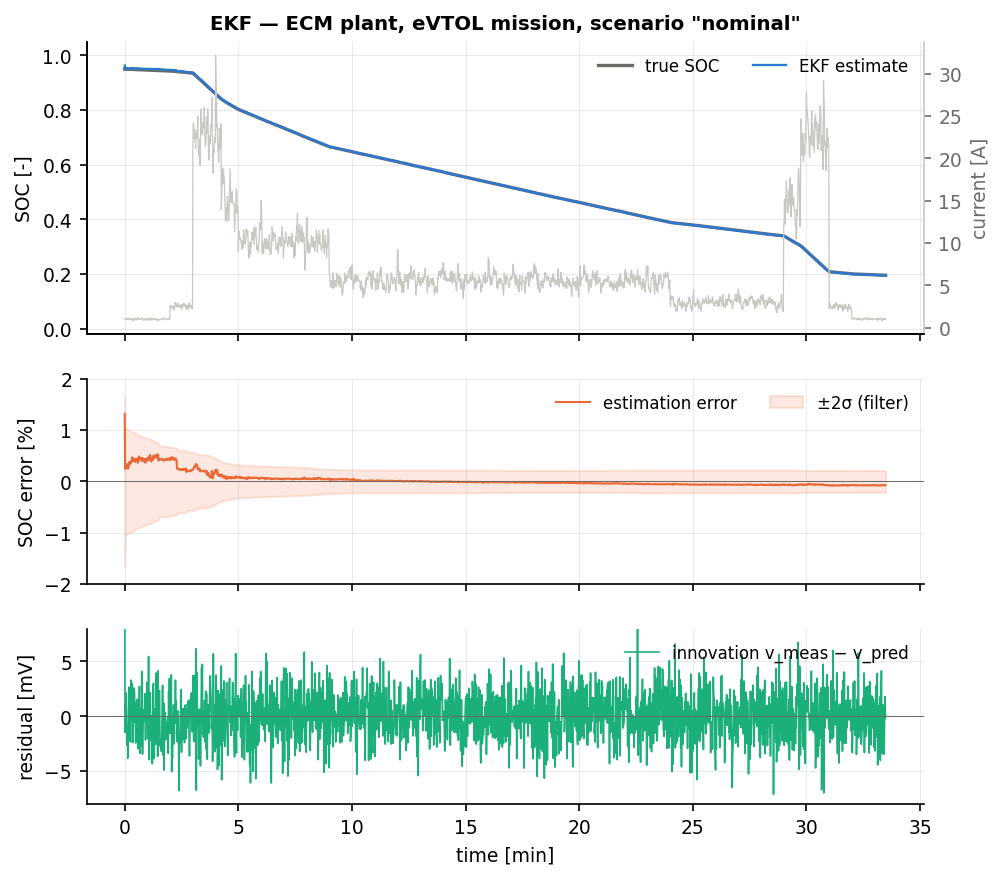
\includegraphics[width=\textwidth]{figures/cell_EKF_nominal.png}
\caption{EKF on the nominal eVTOL mission: true and estimated SOC (top), estimation error with the $\pm 2\sigma$ band when available (middle), voltage residual (bottom).}
\end{figure}
\begin{figure}[H]\centering
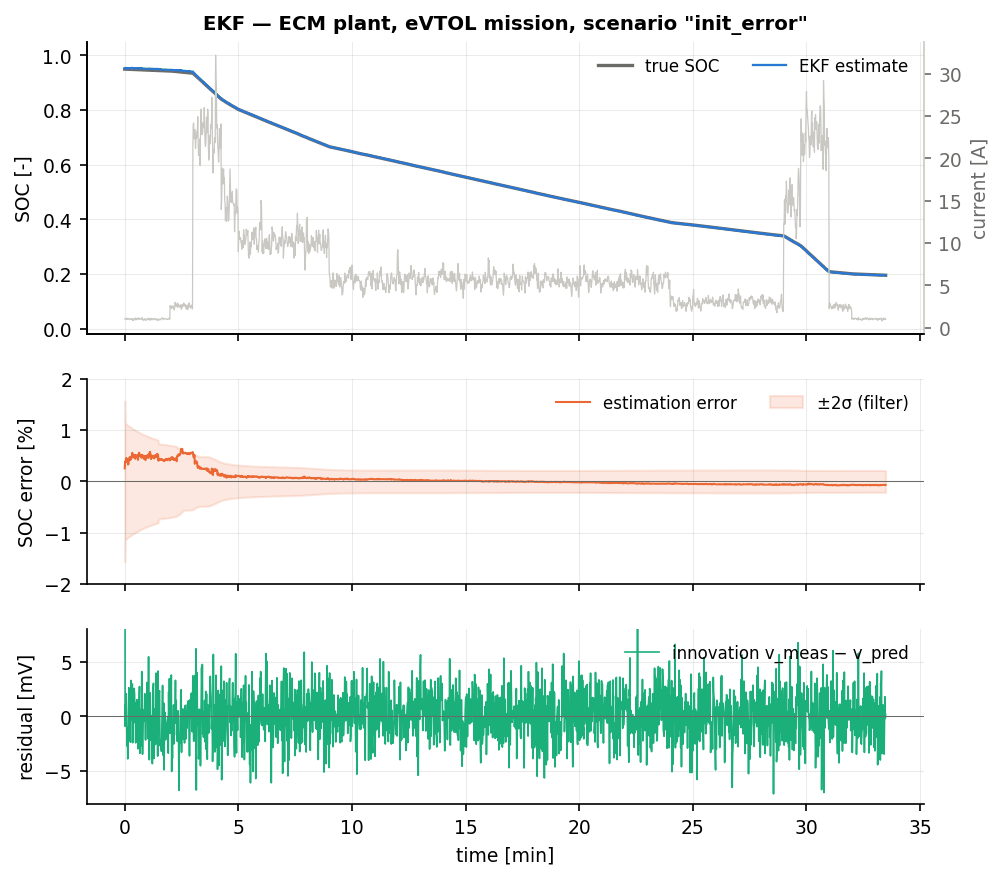
\includegraphics[width=\textwidth]{figures/cell_EKF_init_error.png}
\caption{EKF with a 35\,\% initial SOC error.}
\end{figure}
\begin{figure}[H]\centering
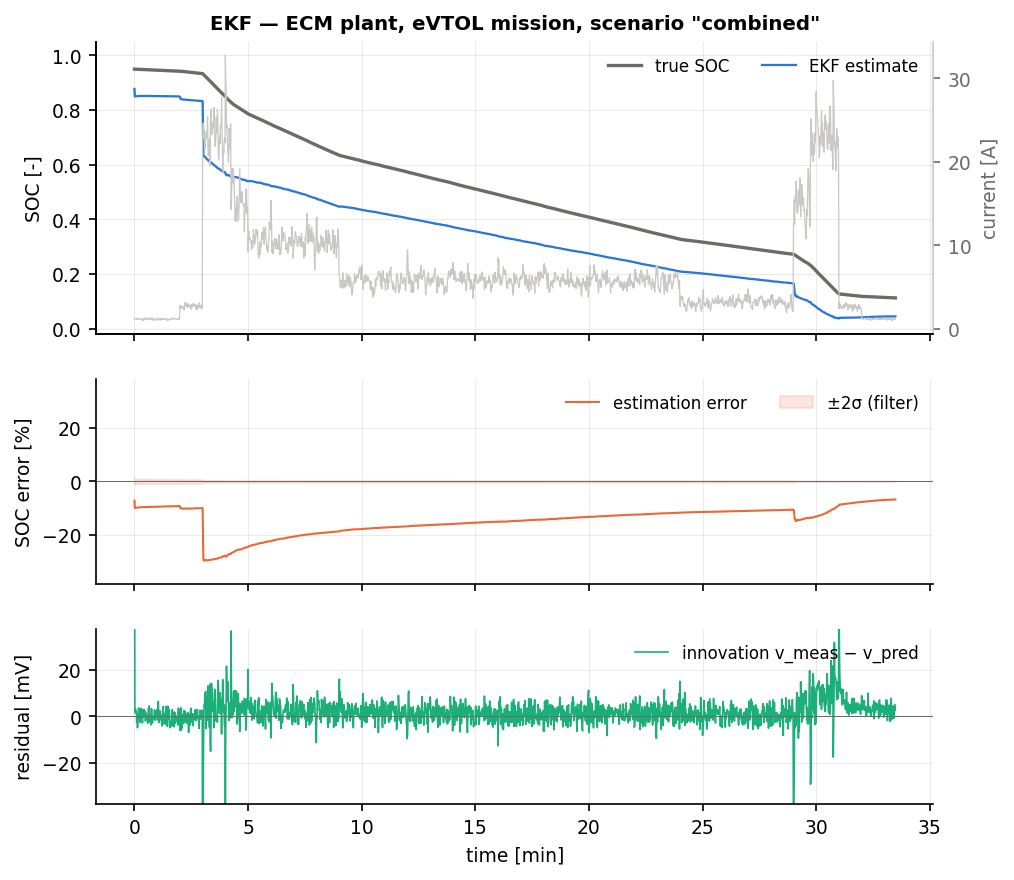
\includegraphics[width=\textwidth]{figures/cell_EKF_combined.png}
\caption{EKF on the \texttt{combined} scenario ($-25\,\%$ initial SOC error, $0.15$\,A current bias, $10\,\%$ capacity loss, $0^\circ$C): the covariance collapses after the first update and the estimate is locked in.}
\end{figure}

All numbers quoted here are three-seed means in per cent SOC, as printed in the table.

On the nominal eVTOL mission the EKF reaches $\text{RMSE} = 0.15\,\%$ over the whole run and
$0.05\,\%$ in steady state, with a voltage-residual RMSE of $0.79$\,mV --- essentially the
sensor noise floor ($\sigma_v = 2$\,mV, quantised at 1\,mV) --- and a maximum error of
$1.07\,\%$. The $-35\,\%$ initial SOC error is removed in a single sample
($t_{\text{conv}} = 0$\,s, $\text{RMSE}_{\text{ss}} = 0.05\,\%$): because the mission begins at
low current and $\Pminus_{\soc\soc} = 10^{-2}$ is four orders of magnitude larger than
$\mR/\mH^2\approx10^{-5}$, the first innovation of $0.28$\,V is almost entirely absorbed by
$\soc$. This is the behaviour that makes the EKF hard to beat on \emph{well-posed} problems and
it is worth stating explicitly: the local linearisation is not a handicap when the prior is
tight or the residual is small.

The failure modes are all consequences of Assumption~\ref{as:ekf-lin} plus the over-confidence
of \eqref{eq:ekf-S}. \texttt{current\_bias} ($0.25$\,A offset, $+2\,\%$ gain) settles at
$0.61\,\%$: the bias is unobservable from a single voltage measurement without an augmented
state, so the filter trades it against the OCV, exactly as predicted
by~\cite{zhao2017observability,lin2018sensorbias}. \texttt{aged\_cell} ($15\,\%$ capacity loss)
gives $1.52\,\%$ and \texttt{param\_mismatch} ($R_0$ at $70\,\%$, $R_1$ at $130\,\%$, $\tau_2$
at $150\,\%$) $1.36\,\%$ --- both are model errors that the filter can only absorb by biasing
$\soc$. \texttt{preisach} is now benign ($0.58\,\%$ whole-run, $0.20\,\%$ steady state,
$t_{\text{conv}} = 16$\,s): with the corrected sign convention of the Preisach plant (charging
branch above the discharging branch) the one-state hysteresis model of the ECM captures most of
the loop, and what remains is a $0.2\,\%$ bias rather than the large offset seen before the
correction.

The interesting failure is \texttt{combined} ($-25\,\%$ initial error, $0.15$\,A current bias,
$10\,\%$ capacity loss, $0^\circ$C): $\text{RMSE}_{\text{ss}} = 12.44\,\%$, a peak error of
$29.6\,\%$ and the convergence criterion is never met. The mechanism is visible in the state
trace. At $k=0$ the filter corrects from $\soc = 0.70$ to $0.877$ and, following
\eqref{eq:ekf-cu}, collapses the standard deviation from $0.10$ to $0.0065$ --- a $15\times$
reduction that the linearisation does \emph{not} justify, because over a $\sigma_\soc = 0.1$
prior the OCV curve is far from affine. The remaining $7\,\%$ error is now locked in: $20$\,s
later the filter is confident and the gain is too small to move. During the hover segment the
aged cell's $25\,\%$ higher $R_0$ (ageing raises $R_0$ by $2.5\times$ the capacity-loss
fraction) produces an extra $0.2$\,V of ohmic drop at $22$\,A, which the filter attributes to
SOC ($0.2/0.8\approx0.25$), and the estimate is driven to $0.54$ against a truth of $0.79$.
Every filter that inflates $\mS$ to account for the OCV curvature --- the UKF
(Chapter~\ref{ch:ukf}, $1.19\,\%$), the second-order EKF (Chapter~\ref{ch:soekf}, $1.28\,\%$),
the IPLF (Chapter~\ref{ch:iplf}, $1.72\,\%$) and the IEKF (Chapter~\ref{ch:iekf}, $2.13\,\%$)
--- survives this scenario. The information filter, the square-root EKF and the U-D filter
(Chapters~\ref{ch:eif}, \ref{ch:srekf}, \ref{ch:udekf}) reproduce the EKF result to $10^{-11}$,
as they must: they are the same estimator in different arithmetic.

\paragraph{SPM plant: structured model error.}
\begin{figure}[H]\centering
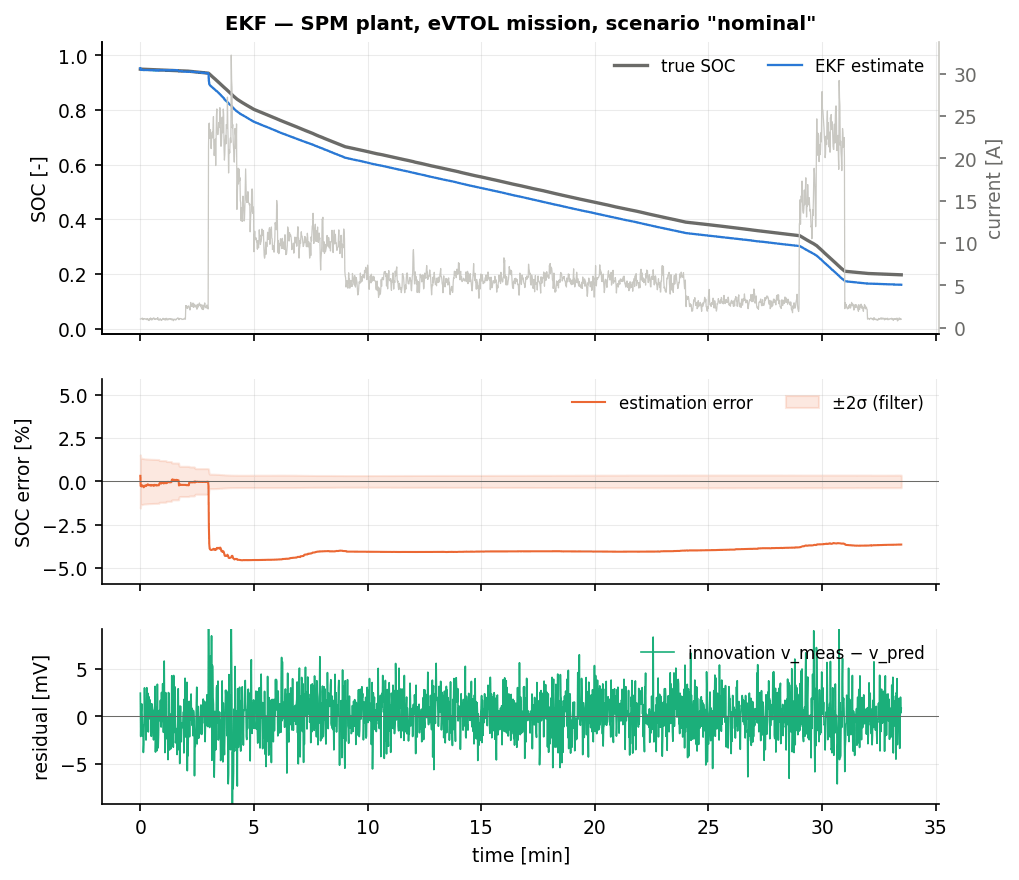
\includegraphics[width=\textwidth]{figures/cellspm_EKF_nominal.png}
\caption{EKF on the nominal mission with the electrochemical (SPM) plant. The estimate carries a persistent bias of about $4\,\%$ SOC even though the voltage residual stays at $1$\,mV.}
\end{figure}
The SPM block of the table is a different kind of test. The plant is the electrochemical
single-particle model; the estimator still runs a 2-RC equivalent circuit, fitted to that plant,
which leaves a \emph{structured} residual of about $4$\,mV (Butler--Volmer kinetics and
solid-phase diffusion that no 2-RC circuit can reproduce) and a slow second branch,
$\tau_2 = 556$\,s. Over a $33$-minute mission a $556$\,s pole barely relaxes, so $v_2(t)$ is
close to an affine ramp --- and so is $\ocv(\soc(t))$ while the cell discharges at a roughly
constant rate. The two channels through which the measurement sees the state,
$(\partial\ocv/\partial\soc)\,\delta\soc$ and $-\delta v_2$, are therefore nearly collinear in
the information accumulated over the flight: the pair $(\soc, v_2)$ is close to unobservable,
and no filter can decide whether a persistent few-millivolt residual belongs to the slow RC
branch or to the state of charge. Because that direction is weakly observable, a $4$\,mV
structured error maps onto \emph{several per cent} of SOC instead of the
$4\,\text{mV}/0.8\,\text{V}\approx0.5\,\%$ a well-conditioned channel would give. This
$(\soc,v_2)$ ambiguity, not the size of the residual, is the mechanism behind the
$3.7$--$4.6\,\%$ band in which the whole classical family sits.

The EKF sits at $3.73\,\%$ steady state on SPM \texttt{nominal} --- seventy times its ECM
figure --- while its voltage residual is only $1.02$\,mV, barely above the ECM value. That
combination is the signature of the ambiguity: the filter fits the voltage almost perfectly and
is nevertheless wrong about SOC by $4\,\%$, because it has paid for the fit with $v_2$ and
$\soc$ in the wrong proportion. Nothing diverges and $t_{\text{conv}} = 0$ everywhere (the
error is a bias, not a drift). \texttt{cold} is the worst case at $7.35\,\%$: at $0^\circ$C the
diffusion overpotential the ECM cannot represent is largest, and the $\tau_2$ branch is slower
still. \texttt{outliers} is, paradoxically, the \emph{best} SPM scenario ($1.99\,\%$): the
corrupted samples widen the effective innovation covariance and stop the filter committing so
hard to the ambiguous direction. Among the filters of this chapter's family the EKF is at the
good end of the band --- the tighter its linearisation, the less weight it puts on the badly
conditioned OCV channel --- and only the frozen-linearisation LKF (Chapter~\ref{ch:lkf},
$1.72\,\%$) and the second-order EKF ($3.52\,\%$) do better.

\section{Summary}
Use the EKF when the model is differentiable, the Jacobians are cheap and the prior is tight
relative to the curvature of $f$ and $h$; on the ECM plant that covers eleven of the twelve
scenarios at a cost of $0.44$--$0.48\,\SI{}{\micro\second}$ per step. Do not use it when a large
prior uncertainty meets a curved measurement function, because the first-order innovation
covariance \eqref{eq:ekf-S} will make the filter over-confident and lock in the error --- the
\texttt{combined} scenario is the object lesson. On a plant whose physics the ECM cannot
represent (the SPM rows) no amount of filtering fixes a $4\,\%$ bias that lives in a nearly
unobservable direction; that needs a better model or an augmented state, not a better filter.
If the same code has to survive a single-precision or fixed-point target, prefer the
algebraically identical U-D or square-root implementations; they cost nothing extra in accuracy
and remove the definiteness question entirely.

% Copyright 2026 Sreeram Anil
% SPDX-License-Identifier: CC-BY-4.0
% =============================================================================
%  Unscented Kalman filter — classical Kalman family
% =============================================================================
\chapter{Unscented Kalman Filter (UKF)}
\label{ch:ukf}

\section*{At a glance}
\begin{tabular}{@{}l>{\raggedright\arraybackslash}p{0.76\textwidth}@{}}
Family & classical Kalman (sigma-point) \\
Header & \texttt{include/estkit/filters/ukf.hpp} \\
Registered name & \texttt{UKF} \\
State dimension & $n_x = 4$ (cell model) --- generic in $n_x, n_u, n_y$ \\
Sigma points & $2n_x+1 = 9$ \\
Cost per step & $\mathcal{O}(n_x^3)$ plus $2(2n_x{+}1)$ model calls; $1.34$--$1.46\,\SI{}{\micro\second}$/step \\
Primary references & \cite{julier2000newmethod,wan2000ukf,julier2004unscented,plett2006spkf1} \\
\end{tabular}

\section{Motivation and aerospace/BMS relevance}
The EKF replaces a nonlinear map by its tangent. Julier and Uhlmann's observation was that
it is easier to approximate a \emph{distribution} than a \emph{function}: pick a small,
deterministic set of points whose sample mean and covariance match the prior exactly, push
them through the true nonlinearity, and read off the transformed moments. No Jacobian is ever
needed, the result is accurate to third order in the Taylor sense for any nonlinearity (and
to second order for the covariance), and the same code works for models that are not
differentiable at all --- look-up tables, saturations, \code{if} statements.

For battery management this matters because the measurement map contains the OCV curve, which
is stored as a table and whose curvature is exactly what the EKF's linearisation discards.
Plett's sigma-point companion papers~\cite{plett2006spkf1,plett2006spkf2} report consistent
improvements over the EKF on lithium-polymer packs and the same qualitative result appears
here: on the hardest benchmark scenario the UKF is the only one of the two baselines that
keeps a usable estimate. In flight-control heritage the same argument is made for attitude
and navigation filters, where the UKF has become the default when the dynamics are stiff or
the attitude error is large~\cite{crassidis2007survey}.

\section{Problem statement and assumptions}
Same model as \eqref{eq:ekf-proc}--\eqref{eq:ekf-meas}: additive Gaussian process and
measurement noise, state $\vx_k\in\real^{n_x}$, input $\vu_k$, measurement
$\vy_k\in\real^{n_y}$. The UKF additionally assumes that the filtering density can be
summarised by its first two moments (the \emph{assumed-density} or Gaussian-filter
assumption, \cite{ito2000gaussian}) but makes no differentiability assumption on $f$ or $h$.
It does assume that $\mP$ is positive definite so that a matrix square root exists.

\section{Derivation}
\paragraph{The unscented transform.} Let $\vx\sim\N{\xhat}{\mP}$, $\mP = \mL\mL^\T$ with
$\mL$ a Cholesky factor, and let $g:\real^{n_x}\to\real^{m}$. Define the scaling parameters
$\alpha\in(0,1]$, $\kappa\ge -n_x$, $\beta\ge 0$ and
\begin{equation}
\lambda = \alpha^2 (n_x+\kappa) - n_x, \qquad c = n_x + \lambda = \alpha^2(n_x+\kappa).
\label{eq:ukf-lambda}
\end{equation}
The $2n_x+1$ sigma points and their two weight sets are
\begin{align}
\mathcal{X}_0 &= \xhat, &
\mathcal{X}_i &= \xhat \pm \left(\sqrt{c\,\mP}\right)_{i}, \quad i = 1,\dots,2n_x,
\label{eq:ukf-sigma}\\
W_0^{m} &= \frac{\lambda}{c}, &
W_0^{c} &= \frac{\lambda}{c} + 1 - \alpha^2 + \beta, \qquad
W_i^{m} = W_i^{c} = \frac{1}{2c},
\label{eq:ukf-weights}
\end{align}
where $(\cdot)_i$ denotes the $i$-th column of the matrix square root and the sign alternates
over the $2n_x$ points. The weights satisfy $\sum_i W_i^m = 1$ and, by construction,
\begin{equation}
\sum_{i} W_i^m \mathcal{X}_i = \xhat, \qquad
\sum_{i} W_i^c (\mathcal{X}_i - \xhat)(\mathcal{X}_i - \xhat)^\T = \mP + (1-\alpha^2+\beta)\,\bm{0} = \mP
\label{eq:ukf-consistency}
\end{equation}
for the centred point (whose deviation vanishes), so the point set is \emph{consistent} with
the prior for any admissible $(\alpha,\beta,\kappa)$.

Expanding $g$ about $\xhat$ shows that
$\sum_i W_i^m g(\mathcal{X}_i) = \E{g(\vx)} + \mathcal{O}(\text{4th order})$: the first and
third order terms cancel by the symmetry of the point set and the second-order term is
captured exactly, whereas the EKF captures only the first. The parameter $\beta$ adds a
correction to $W_0^c$ that is exact for the fourth moment of a Gaussian ($\beta = 2$);
$\alpha$ scales the spread of the points, and $\kappa$ is a residual degree of freedom
usually set to $0$ or $3-n_x$~\cite{julier2004unscented}.

\paragraph{Filter recursion (additive noise).} With $\mathcal{X}_i$ generated from
$(\xplus_{k-1},\Pplus_{k-1})$,
\begin{align}
\mathcal{X}^*_i &= f(\mathcal{X}_i, \vu_{k-1}), &
\xminus_k &= \sum_i W_i^m \mathcal{X}^*_i, \label{eq:ukf-tu-mean}\\
\Pminus_k &= \sum_i W_i^c (\mathcal{X}^*_i - \xminus_k)(\mathcal{X}^*_i - \xminus_k)^\T + \mQ. &&
\label{eq:ukf-tu-cov}
\end{align}
Regenerating the points from $(\xminus_k,\Pminus_k)$ and propagating them through $h$,
\begin{align}
\mathcal{Y}_i &= h(\mathcal{X}_i, \vu_k), \qquad \yhat_k = \sum_i W_i^m \mathcal{Y}_i,
 \label{eq:ukf-ymean}\\
\mP_{yy} &= \sum_i W_i^c (\mathcal{Y}_i-\yhat_k)(\mathcal{Y}_i-\yhat_k)^\T + \mR, \qquad
\mP_{xy} = \sum_i W_i^c (\mathcal{X}_i-\xminus_k)(\mathcal{Y}_i-\yhat_k)^\T,
 \label{eq:ukf-pyy}\\
\mK_k &= \mP_{xy}\mP_{yy}\inv, \qquad
\xplus_k = \xminus_k + \mK_k(\vy_k - \yhat_k), \qquad
\Pplus_k = \Pminus_k - \mK_k \mP_{yy}\mK_k^\T. \label{eq:ukf-mu}
\end{align}
Equation \eqref{eq:ukf-mu} is the same Gaussian conditioning step as in the EKF with
$\mH\Pminus$ replaced by the \emph{statistically} linearised cross-covariance $\mP_{xy}^\T$,
which is why the UKF is often described as a statistical-linear-regression filter --- a view
made explicit in Chapter~\ref{ch:iplf}.

\begin{remark}[Why $W_0^c$ is negative and why it matters here]\label{rm:ukf-w0}
With the benchmark defaults $\alpha=0.1$, $\beta=2$, $\kappa=0$ and $n_x=4$ one gets
$c = 0.04$, $W_0^m = -99$, $W_0^c = -96.01$ and $W_{i\ge1}=12.5$. The points sit at only
$0.2\sigma$ from the mean, so the transform samples the nonlinearity locally, but the large
weights amplify the second difference. For a scalar measurement with curvature
$c_h = \partial^2 h/\partial \soc^2$ the resulting predicted-measurement variance is
$\mP_{yy} \approx \mH\Pminus\mH^\T + \tfrac12 c_h^2\sigma_\soc^4 + \mR$: exactly the
second-order term that the EKF omits. At $\sigma_\soc = 0.1$ and $c_h\approx -6$\,V this adds
$1.9\times10^{-3}$\,V$^2$ to an $\mS$ of $5.6\times10^{-3}$\,V$^2$ --- a $34\,\%$ inflation
that stops the filter from collapsing $\mP$ after the first update.
\end{remark}

\section{Algorithm}
\begin{algorithm}[H]
\caption{UKF --- one sampling period (additive noise)}
\begin{algorithmic}[1]
\Require $\xplus_{k-1}, \Pplus_{k-1}, \vu_{k-1}, \vy_k, \vu_k$, parameters $\alpha,\beta,\kappa$
\State $\lambda \gets \alpha^2(n_x+\kappa)-n_x$; \; $\mL \gets \operatorname{chol}\!\big((n_x{+}\lambda)\Pplus_{k-1}\big)$
\State $\mathcal{X}_0\gets\xplus_{k-1}$; \; $\mathcal{X}_{i},\mathcal{X}_{i+n_x} \gets \xplus_{k-1} \pm \mL_{:,i}$; weights from \eqref{eq:ukf-weights}
\State \textbf{Time update:} $\mathcal{X}_i \gets f(\mathcal{X}_i,\vu_{k-1})$;\;
       $\xminus_k \gets \sum_i W^m_i\mathcal{X}_i$
\State $\Pminus_k \gets \sum_i W^c_i(\mathcal{X}_i-\xminus_k)(\cdot)^\T + \mQ$; symmetrise
\State \textbf{Regenerate} $\mathcal{X}_i$ from $(\xminus_k,\Pminus_k)$
\State $\mathcal{Y}_i \gets h(\mathcal{X}_i,\vu_k)$; \; $\yhat_k \gets \sum_i W^m_i \mathcal{Y}_i$
\State $\mP_{yy} \gets \sum_i W^c_i (\mathcal{Y}_i-\yhat_k)(\cdot)^\T + \mR$; \;
       $\mP_{xy} \gets \sum_i W^c_i (\mathcal{X}_i-\xminus_k)(\mathcal{Y}_i-\yhat_k)^\T$
\State $\mK\gets\mP_{xy}\mP_{yy}\inv$; \;
       $\xplus_k \gets \xminus_k + \mK(\vy_k-\yhat_k)$; \;
       $\Pplus_k \gets \Pminus_k - \mK\mP_{yy}\mK^\T$
\State \textbf{if} constraints enabled \textbf{then} $\xplus_k \gets \Pi(\xplus_k)$
\Ensure $\xplus_k, \Pplus_k$
\end{algorithmic}
\end{algorithm}

\section{Application to the battery model}
The cell dynamics $f$ are \emph{affine} in $\vx$ (the coefficients $a_1,a_2,a_h$ depend only
on $\vu$), so the unscented time update reproduces the EKF time update exactly; all the
difference is in the measurement update, where $h$ contains the OCV table. The cost is
$2\times 9 = 18$ evaluations of the cell model per step against 2 for the EKF, which is the
entire explanation of the $\approx 3\times$ runtime ratio
($1.34$--$1.46\,\SI{}{\micro\second}$ versus $0.44$--$0.48\,\SI{}{\micro\second}$).

Benchmark options: $\alpha = 0.1$, $\beta = 2$, $\kappa = 0$,
\code{apply\_constraints = true}, \code{q\_scale = r\_scale = 1}. The choice $\alpha=0.1$ is
the value recommended for a ``small spread around the mean'' in~\cite{wan2000ukf} and is the
one Plett uses for cells~\cite{plett2006spkf1}. Note that $\Pplus$ can in principle lose
positive definiteness because $W_0^c<0$; here it never did, and the square-root variant of
Chapter~\ref{ch:srukf} removes the possibility altogether.

\section{Implementation notes}
\code{cholesky\_safe} adds a scaled diagonal jitter and retries up to eight times, so the
factorisation in \eqref{eq:ukf-sigma} cannot abort. \code{predict\_measurement} regenerates
the sigma set from the current $(\xminus,\Pminus)$ so that the reported voltage prediction is
the sigma-mean $\yhat$ and not $h(\xminus)$ --- the two differ by $\approx 30$\,mV at
$\sigma_\soc = 0.1$, which is the second-order correction of Remark~\ref{rm:ukf-w0} and is
precisely what the benchmark's voltage-residual metric should see. The filter stores the
sigma set ($9\times 4$ reals) and weights inside the object;
\code{sizeof(Ukf<EcmModel>)} is 4760\,bytes. On a Cortex-M7 the cost is dominated by the 18
OCV table look-ups and 9 exponential calls; a look-up-table exponential brings this to
$\approx \SI{30}{\micro\second}$, still negligible at \SI{10}{\hertz}.

\section{Benchmark results}
% Copyright 2026 Sreeram Anil
% SPDX-License-Identifier: CC-BY-4.0
\begin{table}[H]\centering\footnotesize\setlength{\tabcolsep}{4pt}
\caption{UKF: cell-level benchmark on the eVTOL mission (mean over seeds; RMSE and max error in \% SOC; $t_\mathrm{conv}$: first time the error stays below 2\,\% for 60\,s, -- = never; EKF reference: steady-state RMSE of the plain EKF on the same data).}\label{tab:cell_UKF}
\begin{tabular}{llrrrrrcrr}\toprule
plant & scenario & RMSE & RMSE$_\mathrm{ss}$ & max & $t_\mathrm{conv}$ [s] & RMSE$_v$ [mV] & div. & EKF ref. & ns/step \\ \midrule
ECM & nominal & 0.20 & 0.04 & 4.02 & 0 & 1.08 & no & 0.05 & 1442 \\
ECM & init\_error & 0.17 & 0.07 & 3.30 & 0 & 2.06 & no & 0.05 & 1447 \\
ECM & current\_bias & 0.58 & 0.57 & 3.83 & 0 & 1.11 & no & 0.61 & 1442 \\
ECM & noise\_step & 0.22 & 0.11 & 4.02 & 0 & 2.98 & no & 0.12 & 1444 \\
ECM & outliers & 0.48 & 0.18 & 4.94 & 8 & 2.21 & no & 0.21 & 1447 \\
ECM & cold & 0.27 & 0.07 & 4.02 & 0 & 2.03 & no & 0.16 & 1439 \\
ECM & hot & 0.21 & 0.03 & 4.03 & 0 & 0.91 & no & 0.03 & 1441 \\
ECM & aged\_cell & 1.10 & 1.36 & 4.40 & 0 & 3.88 & no & 1.52 & 1441 \\
ECM & param\_mismatch & 1.29 & 1.37 & 4.27 & 0 & 2.92 & no & 1.36 & 1441 \\
ECM & sensor\_dropout & 1.39 & 0.86 & 4.77 & 0 & 1.90 & no & 0.46 & 1437 \\
ECM & preisach & 1.35 & 0.23 & 5.53 & 214 & 1.20 & no & 0.20 & 1440 \\
ECM & combined & 1.23 & 1.19 & 7.70 & 0 & 4.68 & no & 12.44 & 1456 \\
\midrule
SPM & nominal & 3.95 & 3.96 & 5.06 & 0 & 1.29 & no & 3.73 & 1377 \\
SPM & init\_error & 4.62 & 4.54 & 5.83 & -- & 2.12 & no & 3.81 & 1352 \\
SPM & current\_bias & 5.77 & 6.46 & 7.22 & 0 & 1.36 & no & 5.69 & 1368 \\
SPM & noise\_step & 3.57 & 3.24 & 5.06 & 0 & 3.24 & no & 3.30 & 1379 \\
SPM & outliers & 1.70 & 1.76 & 8.23 & 0 & 2.55 & no & 1.99 & 1342 \\
SPM & cold & 8.20 & 8.29 & 10.75 & -- & 4.62 & no & 7.35 & 1365 \\
SPM & hot & 2.32 & 2.36 & 4.41 & 0 & 1.04 & no & 2.16 & 1367 \\
SPM & param\_mismatch & 4.75 & 4.95 & 5.63 & 0 & 2.12 & no & 3.13 & 1365 \\
SPM & sensor\_dropout & 7.06 & 7.26 & 8.32 & 0 & 2.10 & no & 5.31 & 1368 \\
\bottomrule\end{tabular}\end{table}

\begin{figure}[H]\centering
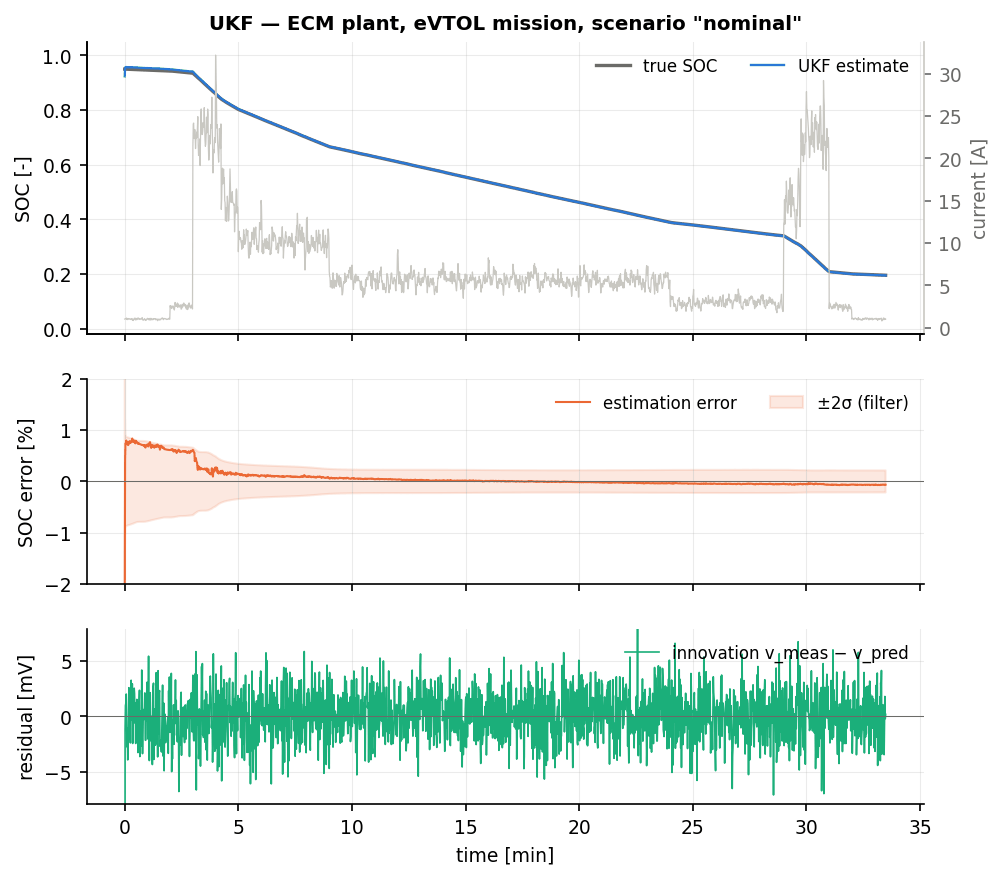
\includegraphics[width=\textwidth]{figures/cell_UKF_nominal.png}
\caption{UKF on the nominal eVTOL mission: true and estimated SOC (top), estimation error with the $\pm 2\sigma$ band when available (middle), voltage residual (bottom).}
\end{figure}
\begin{figure}[H]\centering
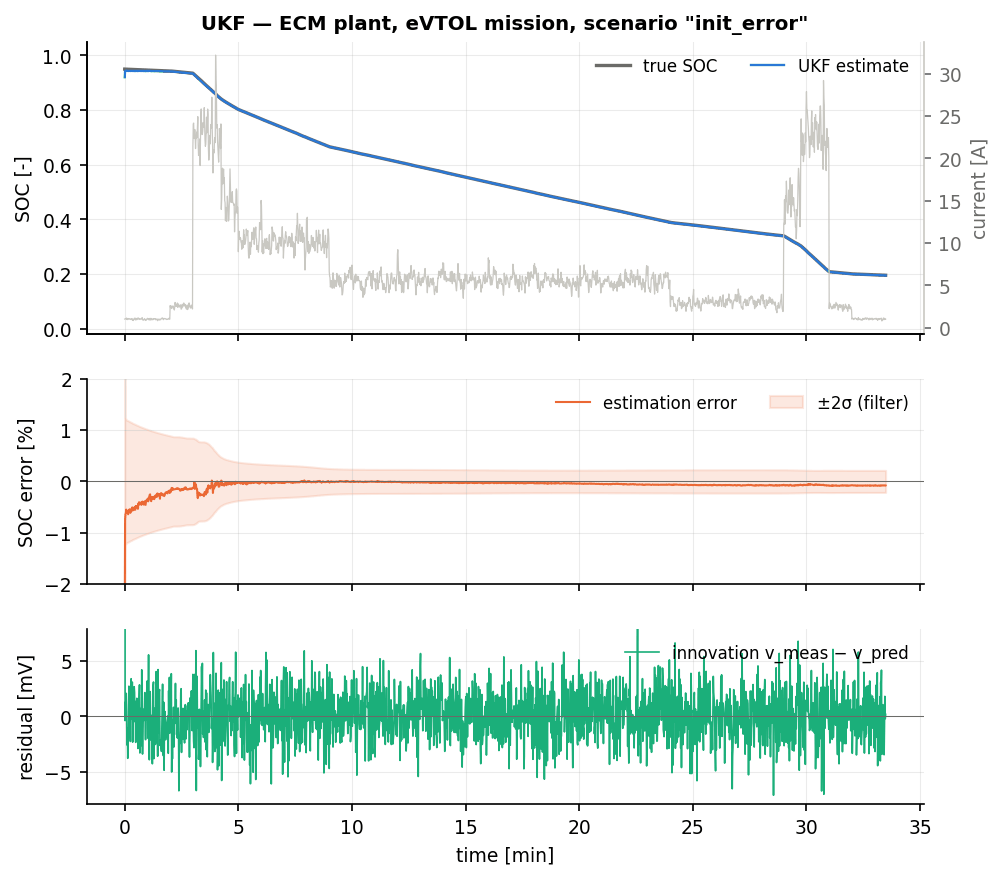
\includegraphics[width=\textwidth]{figures/cell_UKF_init_error.png}
\caption{UKF with a 35\,\% initial SOC error.}
\end{figure}
\begin{figure}[H]\centering
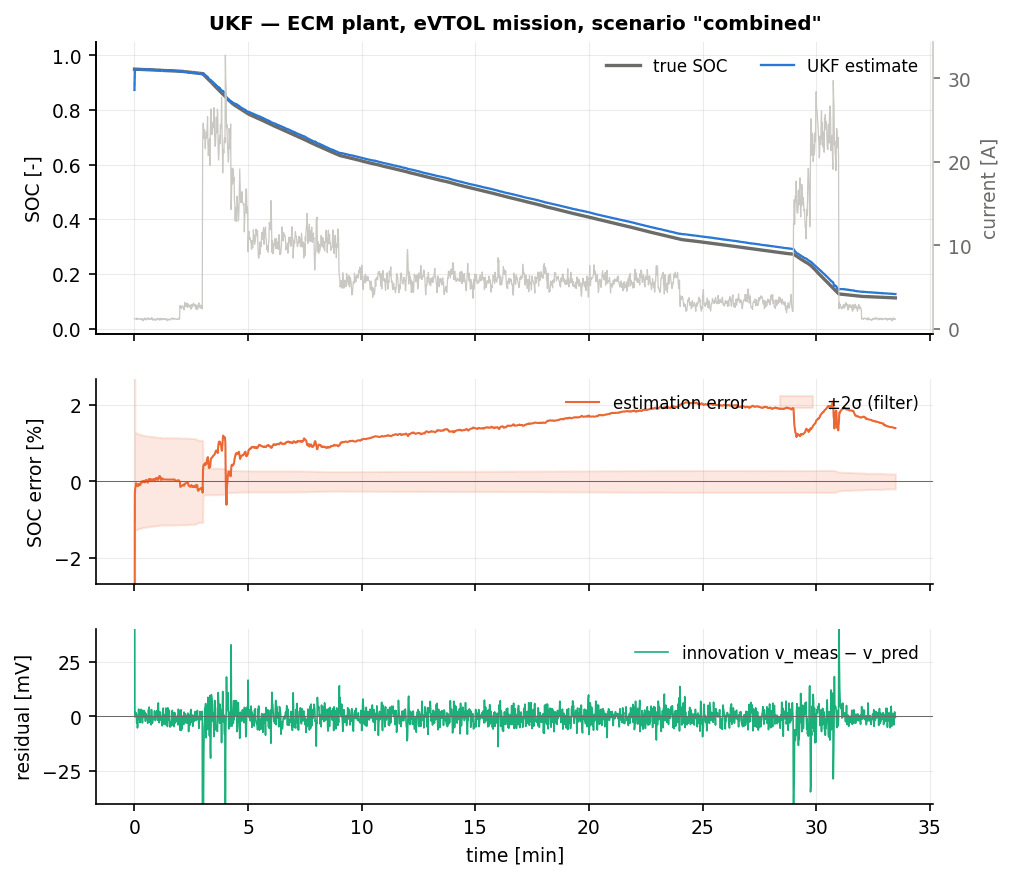
\includegraphics[width=\textwidth]{figures/cell_UKF_combined.png}
\caption{UKF on the \texttt{combined} scenario: the inflated predicted-measurement variance keeps the gain alive and the estimate locks onto the truth within seconds, where the EKF never recovers.}
\end{figure}

All numbers are three-seed means in per cent SOC.

Nominal performance is marginally better than the EKF's in steady state
($\text{RMSE}_{\text{ss}} = 0.04\,\%$ against $0.05\,\%$) but worse over the whole run
($0.20\,\%$ against $0.15\,\%$), with a maximum error of $4.02\,\%$ against $1.07\,\%$. Both
come from the same place: the transient of the first few seconds, where $\mP$ is still at its
initial value and the second-order term of Remark~\ref{rm:ukf-w0} makes the filter deliberately
cautious. With the $-35\,\%$ initial error the caution costs a little
($0.07\,\%$ steady state against the EKF's $0.05\,\%$) but both converge in the first sample.

The decisive result is \texttt{combined}, where the EKF reaches
$\text{RMSE}_{\text{ss}} = 12.44\,\%$ and never converges while the UKF reaches $1.19\,\%$ and
converges immediately --- the best figure of all fifteen filters on that scenario, marginally
ahead of the second-order EKF ($1.28\,\%$) and the IPLF ($1.72\,\%$). The state trace explains
it completely: after the first update the EKF reports $\sigma_\soc = 0.0065$ and the UKF
$\sigma_\soc = 0.0416$; $20$\,s later the UKF has pulled the estimate onto the truth
($0.9488$ against a true $0.9488$) whereas the EKF is stuck at $0.852$ and stays wrong for the
rest of the flight. The extra variance in $\mP_{yy}$ --- a genuine second-order effect, not a
fudge factor --- is what keeps the gain alive long enough to find the right answer. Note
however that this is an \emph{indirect} benefit of $\alpha = 0.1$: the same inflation appears
explicitly and more cheaply in the second-order EKF (Chapter~\ref{ch:soekf}).

Elsewhere the UKF and the EKF are close, with the UKF ahead on the scenarios where extra
caution helps --- \texttt{cold} $0.07\,\%$ against $0.16\,\%$, \texttt{aged\_cell} $1.36\,\%$
against $1.52\,\%$, \texttt{outliers} $0.18\,\%$ against $0.21\,\%$ --- and behind where it does
not: \texttt{sensor\_dropout} $0.86\,\%$ against $0.46\,\%$ and \texttt{preisach} $0.23\,\%$
against $0.20\,\%$ with a convergence time of $214$\,s against $16$\,s. The
\texttt{preisach} scenario changed character when the plant's hysteresis sign convention was
corrected: it is now a mild $0.2\,\%$ bias for the whole family rather than a differentiator,
and what the UKF loses there is convergence speed, not accuracy.

\paragraph{SPM plant: structured model error.}
\begin{figure}[H]\centering
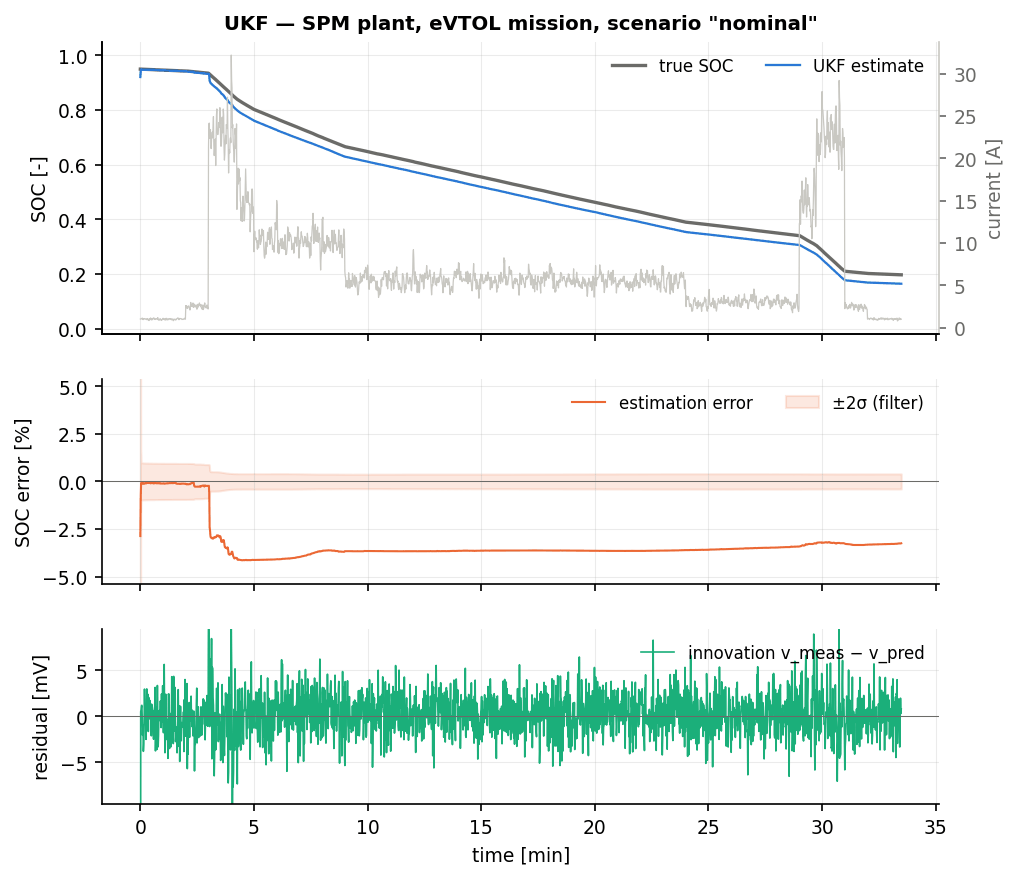
\includegraphics[width=\textwidth]{figures/cellspm_UKF_nominal.png}
\caption{UKF on the nominal mission with the electrochemical (SPM) plant.}
\end{figure}
The SPM block of the table is a different kind of test. The plant is the electrochemical
single-particle model; the estimator still runs a 2-RC equivalent circuit, fitted to that plant,
which leaves a \emph{structured} residual of about $4$\,mV (Butler--Volmer kinetics and
solid-phase diffusion that no 2-RC circuit can reproduce) and a slow second branch,
$\tau_2 = 556$\,s. Over a $33$-minute mission a $556$\,s pole barely relaxes, so $v_2(t)$ is
close to an affine ramp --- and so is $\ocv(\soc(t))$ while the cell discharges at a roughly
constant rate. The two channels through which the measurement sees the state,
$(\partial\ocv/\partial\soc)\,\delta\soc$ and $-\delta v_2$, are therefore nearly collinear in
the information accumulated over the flight: the pair $(\soc, v_2)$ is close to unobservable,
and no filter can decide whether a persistent few-millivolt residual belongs to the slow RC
branch or to the state of charge. Because that direction is weakly observable, a $4$\,mV
structured error maps onto \emph{several per cent} of SOC instead of the
$4\,\text{mV}/0.8\,\text{V}\approx0.5\,\%$ a well-conditioned channel would give. This
$(\soc,v_2)$ ambiguity, not the size of the residual, is the mechanism behind the
$3.7$--$4.6\,\%$ band in which the whole classical family sits.

The UKF sits at $3.96\,\%$ on SPM \texttt{nominal}, slightly \emph{worse} than the EKF's
$3.73\,\%$, and the gap widens on the harder rows: \texttt{cold} $8.29\,\%$ against $7.35\,\%$,
\texttt{param\_mismatch} $4.95\,\%$ against $3.13\,\%$, \texttt{sensor\_dropout} $7.26\,\%$
against $5.31\,\%$. This reverses the ECM ordering and it follows directly from the ambiguity
argument: the unscented transform performs a statistical regression of $h$ over the prior, and
a regression puts \emph{more} weight on the OCV channel than a tangent does, so it commits
harder to the direction that carries the structured error. The exception is
\texttt{outliers}, where the UKF's extra caution again pays ($1.76\,\%$ against $1.99\,\%$).
The general lesson is worth stating: better moment propagation is a remedy for nonlinearity,
not for a model that is structurally wrong, and on the SPM plant it is mildly
counter-productive.

\section{Summary}
The UKF costs about three times an EKF step and buys derivative-free implementation plus
second-order accurate moments. On this cell model that is worth little in most ECM scenarios
--- the dynamics are affine and the prior is usually tight --- and worth everything in the one
scenario where a large prior meets the curved OCV characteristic, where it is the best filter
of the fifteen. Choose it when Jacobians are unavailable or unreliable, when the initial SOC
uncertainty is large (first power-up, after a pack swap), or when the same filter must also
carry parameters. Do not expect it to fix biased sensors, a wrong capacity, or structured model
error: on the SPM plant it is slightly worse than the plain EKF.

% Copyright 2026 Sreeram Anil
% SPDX-License-Identifier: CC-BY-4.0
% =============================================================================
%  Plain (linearised-once) Kalman filter — classical Kalman family
% =============================================================================
\chapter{Linear Kalman Filter on a Frozen Linearisation (LKF)}
\label{ch:lkf}

\section*{At a glance}
\begin{tabular}{@{}l>{\raggedright\arraybackslash}p{0.76\textwidth}@{}}
Family & classical Kalman \\
Header & \texttt{include/estkit/filters/kf\_linear.hpp} \\
Registered name & \texttt{LKF} \\
State dimension & $n_x = 4$ (cell model) --- generic in $n_x, n_u, n_y$ \\
Cost per step & $\mathcal{O}(n_x^3)$, $320$--$336$\,ns/step; gain schedule computable offline \\
Primary references & \cite{kalman1960,kalmanbucy1961,andersonmoore1979,sorenson1970gauss} \\
\end{tabular}

\section{Motivation and aerospace/BMS relevance}
Kalman's 1960 filter is optimal for a \emph{linear} system. Everything else in this report is
an attempt to keep that optimality in the presence of nonlinearity. It is therefore worth
establishing, quantitatively, what happens if one simply ignores the problem: linearise the
cell model once, at power-up, and run the textbook linear filter for the rest of the flight.

This is not a straw man. A time-invariant Kalman filter has properties no nonlinear filter
can offer. Its Riccati recursion does not depend on the data, so $\mP_k$ and $\mK_k$ can be
computed on the ground and stored as a table --- or replaced by their steady-state values
$\mP_\infty, \mK_\infty$, the solution of a discrete algebraic Riccati equation
\cite[\S4.4]{andersonmoore1979}. The flight code is then a fixed-gain observer costing
$n_x n_y$ multiplies per step, with no matrix inversion, no Cholesky, no Jacobian evaluation
and a completely deterministic execution time --- the kind of code that gets certified
quickly. Several production BMS use exactly this structure with a gain scheduled on
temperature. The question this chapter answers is what it costs in accuracy.

\section{Problem statement and assumptions}
The plant is \eqref{eq:ekf-proc}--\eqref{eq:ekf-meas}. The filter is given, once, a
linearisation point $(\vx_0,\vu_{\text{lin}})$ --- in the benchmark the initial estimate and
the cell at rest, $\vu_{\text{lin}} = [0, T_0]^\T$ with $T_0$ the temperature reported at
reset --- and forms the constant matrices
\begin{equation}
\mF = \left.\frac{\partial f}{\partial\vx}\right|_{\vx_0,\vu_{\text{lin}}}, \qquad
\mH = \left.\frac{\partial h}{\partial\vx}\right|_{\vx_0,\vu_{\text{lin}}}, \qquad
\mQ = \mQ(\vx_0,\vu_{\text{lin}}), \qquad
\mR = \mR(\vx_0,\vu_{\text{lin}}).
\label{eq:lkf-frozen}
\end{equation}
\begin{assumption}[Global linearity about one point]\label{as:lkf}
The first-order Taylor expansions of $f$ and $h$ about $\vx_0$ are accurate over the whole
trajectory the state will visit, and the noise statistics do not depend on the operating
point.
\end{assumption}
Assumption~\ref{as:lkf} is much stronger than the EKF's Assumption~\ref{as:ekf-lin} and is,
for a battery discharging from $95\,\%$ to $20\,\%$ SOC, plainly false. Quantifying ``how
false'' is the purpose of the experiment.

\section{Derivation}
Write the affine surrogate model obtained by freezing the Jacobians but keeping the exact
dependence on the (measured) input:
\begin{align}
f(\vx,\vu) &\approx \tilde f(\vx,\vu) := f(\vx_0,\vu) + \mF(\vx - \vx_0), \label{eq:lkf-f}\\
h(\vx,\vu) &\approx \tilde h(\vx,\vu) := h(\vx_0,\vu) + \mH(\vx - \vx_0). \label{eq:lkf-h}
\end{align}
Both are exact in $\vu$ and first order in $\vx$ about $\vx_0$; in particular the
ampere-hour integration and the ohmic term $-R_0(T)i$ are reproduced exactly, so the
surrogate is not a caricature but a genuine linear time-varying-input model. The Kalman
recursion for \eqref{eq:lkf-f}--\eqref{eq:lkf-h} is
\begin{align}
\xminus_k &= \mF\left(\xplus_{k-1} - \vx_0\right) + f(\vx_0, \vu_{k-1}), &
\Pminus_k &= \mF\Pplus_{k-1}\mF^\T + \mQ, \label{eq:lkf-tu}\\
\yhat_k &= h(\vx_0,\vu_k) + \mH(\xminus_k - \vx_0), &
\mS_k &= \mH\Pminus_k\mH^\T + \mR, \label{eq:lkf-ypred}\\
\mK_k &= \Pminus_k\mH^\T\mS_k\inv, &
\xplus_k &= \xminus_k + \mK_k(\vy_k - \yhat_k), \label{eq:lkf-gain}
\end{align}
with the Joseph covariance update \eqref{eq:ekf-joseph}. Because $\mF,\mH,\mQ,\mR$ are
constant, the pair $(\Pminus_k,\mK_k)$ obeys the deterministic Riccati recursion
\begin{equation}
\Pminus_{k+1} = \mF\left[\Pminus_k - \Pminus_k\mH^\T(\mH\Pminus_k\mH^\T+\mR)\inv \mH\Pminus_k\right]\mF^\T + \mQ,
\label{eq:lkf-riccati}
\end{equation}
which, if $(\mF,\mH)$ is detectable and $(\mF,\mQ^{1/2})$ stabilisable, converges to the
unique stabilising solution $\mP_\infty$ of the DARE and the gain to
$\mK_\infty = \mP_\infty\mH^\T(\mH\mP_\infty\mH^\T+\mR)\inv$
\cite[Ch.~4]{andersonmoore1979}. For the cell model $\mF=\diag(1,a_1,a_2,a_h)$ and
$\mH=[\partial\ocv/\partial\soc,\,-1,\,-1,\,M]$; the pair is observable because the first
entry of $\mH$ is non-zero, so the SOC integrator is stabilised through the OCV channel.
\code{estkit} provides \code{dare\_iterate} for the offline computation of
$(\mP_\infty,\mK_\infty)$.

\paragraph{The error this introduces.} The measurement bias committed at state $\vx$ is
\begin{equation}
b(\vx) = h(\vx,\vu) - \tilde h(\vx,\vu) = \ocv(\soc) - \left[\ocv(\soc_0) + \ocv'(\soc_0)(\soc-\soc_0)\right]
 = \tfrac12 \ocv''(\xi)(\soc-\soc_0)^2
\label{eq:lkf-bias}
\end{equation}
for some $\xi$ between $\soc_0$ and $\soc$ --- the deviation of the OCV curve from its
tangent at the linearisation point, not merely the slope error. A persistent measurement
bias $b$ is absorbed by a steady-state SOC error of approximately
$\Delta\soc \approx -b/\ocv'$, since in steady state the filter drives the innovation to
zero. This is the dominant error mechanism of the LKF and it grows quadratically as the cell
discharges away from $\soc_0$.

\section{Algorithm}
\begin{algorithm}[H]
\caption{LKF --- initialisation and one sampling period}
\begin{algorithmic}[1]
\Require at reset: $\vx_0, \mP_0, \vu_{\text{lin}}$
\State \textbf{Once:} $\mF\gets \partial f/\partial\vx|_{\vx_0,\vu_{\text{lin}}}$,\;
       $\mH\gets \partial h/\partial\vx|_{\vx_0,\vu_{\text{lin}}}$,\;
       $\mQ\gets\mQ(\vx_0,\vu_{\text{lin}})$,\; $\mR\gets\mR(\vx_0,\vu_{\text{lin}})$
\State \textbf{Time update:} $\xminus_k\gets f(\vx_0,\vu_{k-1}) + \mF(\xplus_{k-1}-\vx_0)$
\State $\Pminus_k \gets \mF\Pplus_{k-1}\mF^\T+\mQ$; symmetrise
\State \textbf{Predicted measurement:} $\yhat_k \gets h(\vx_0,\vu_k) + \mH(\xminus_k-\vx_0)$
\State \textbf{Measurement update:} $\mS\gets\mH\Pminus_k\mH^\T+\mR$,\;
       $\mK\gets\Pminus_k\mH^\T\mS\inv$
\State $\xplus_k\gets\xminus_k+\mK(\vy_k-\yhat_k)$,\;
       $\Pplus_k\gets(\mI-\mK\mH)\Pminus_k(\mI-\mK\mH)^\T+\mK\mR\mK^\T$
\State \textbf{if} constraints enabled \textbf{then} $\xplus_k\gets\Pi(\xplus_k)$
\Ensure $\xplus_k,\Pplus_k$; \quad (steps 3, 5 may be replaced by the stored $\mK_\infty$)
\end{algorithmic}
\end{algorithm}

\section{Application to the battery model}
The frozen quantities for the nominal benchmark are, at $\soc_0=0.95$, $T_0=298.15$\,K and
$i=0$:
\begin{equation}
\mF = \diag(1,\;0.9802,\;0.99917,\;1), \qquad
\mH = [\,0.7485,\;-1,\;-1,\;0.005\,].
\label{eq:lkf-battery}
\end{equation}
Two entries deserve comment. $\mH_{1}=\partial\ocv/\partial\soc$ at $\soc=0.95$ is
$0.7485$\,V, while over the mission the true slope ranges from $0.71$\,V at $\soc=0.4$ to
$0.93$\,V at $\soc=0.8$ --- a modest $\pm 20\,\%$, so the \emph{slope} alone is not the
problem. The tangent-line \emph{offset} \eqref{eq:lkf-bias} is: integrating the curvature
from $\soc_0 = 0.95$ down to $\soc = 0.20$ accumulates a model voltage error of order
$40$\,mV, i.e. $\Delta\soc \approx 0.05$. Second, $a_h(i{=}0) = 1$: linearising at rest
freezes the hysteresis state as a pure random walk, so its decay is lost.

The \code{u\_lin} option is set by the registry to $[0, T_0]^\T$, i.e. the cell at rest at
the temperature reported at reset; \code{freeze\_noise = true} gives the strictly
time-invariant filter described above (setting it to \code{false} re-evaluates $\mQ,\mR$ at
the current input and was measured to change nothing at all on this benchmark, to four
decimal places, in all scenarios).

\section{Implementation notes}
The implementation keeps $\vx_0$, $\mF$, $\mH$, $\mQ$, $\mR$ as members, so the per-step work
is two $4\times4$ products and one $1\times1$ inverse: $320$--$336$\,ns, the cheapest filter of the
fifteen and $\approx 30\,\%$ faster than the EKF ($443$--$482$\,ns), which must rebuild $\mF$
and $\mH$ every step. \code{sizeof(LinearKf<EcmModel>)} is 4680\,bytes, again dominated by the model copy.
Because $\mP_k$ follows \eqref{eq:lkf-riccati} independently of the data, a flight
implementation would drop $\mP$ entirely and store $\mK_\infty$ (four reals), reducing the
filter to $\xplus = \xminus + \mK_\infty \veps$ --- 4 multiply-accumulates per step. The
float build reproduces the double results exactly to four decimals in every scenario, as
expected for a filter whose covariance never becomes ill-conditioned.

\section{Benchmark results}
% Copyright 2026 Sreeram Anil
% SPDX-License-Identifier: CC-BY-4.0
\begin{table}[H]\centering\footnotesize\setlength{\tabcolsep}{4pt}
\caption{LKF: cell-level benchmark on the eVTOL mission (mean over seeds; RMSE and max error in \% SOC; $t_\mathrm{conv}$: first time the error stays below 2\,\% for 60\,s, -- = never; EKF reference: steady-state RMSE of the plain EKF on the same data).}\label{tab:cell_LKF}
\begin{tabular}{llrrrrrcrr}\toprule
plant & scenario & RMSE & RMSE$_\mathrm{ss}$ & max & $t_\mathrm{conv}$ [s] & RMSE$_v$ [mV] & div. & EKF ref. & ns/step \\ \midrule
ECM & nominal & 3.23 & 1.19 & 6.29 & 0 & 1.13 & no & 0.05 & 334 \\
ECM & init\_error & 3.44 & 2.19 & 6.01 & 0 & 2.24 & no & 0.05 & 332 \\
ECM & current\_bias & 3.74 & 1.36 & 7.15 & 0 & 1.13 & no & 0.61 & 335 \\
ECM & noise\_step & 3.23 & 1.19 & 6.29 & 0 & 2.98 & no & 0.12 & 332 \\
ECM & outliers & 3.24 & 1.19 & 6.41 & 0 & 2.20 & no & 0.21 & 331 \\
ECM & cold & 13.12 & 12.49 & 18.93 & 0 & 3.86 & no & 0.16 & 330 \\
ECM & hot & 2.14 & 1.62 & 3.91 & 0 & 1.02 & no & 0.03 & 329 \\
ECM & aged\_cell & 1.67 & 1.14 & 5.64 & 0 & 4.05 & no & 1.52 & 330 \\
ECM & param\_mismatch & 1.81 & 1.19 & 3.63 & 0 & 2.90 & no & 1.36 & 332 \\
ECM & sensor\_dropout & 3.27 & 1.20 & 6.34 & 0 & 1.75 & no & 0.46 & 330 \\
ECM & preisach & 2.76 & 1.06 & 5.40 & 0 & 1.11 & no & 0.20 & 336 \\
ECM & combined & 6.38 & 7.00 & 11.89 & -- & 5.16 & no & 12.44 & 331 \\
\midrule
SPM & nominal & 1.30 & 1.72 & 2.71 & 0 & 1.05 & no & 3.73 & 330 \\
SPM & init\_error & 0.56 & 0.55 & 1.27 & 0 & 2.18 & no & 3.81 & 321 \\
SPM & current\_bias & 1.96 & 2.65 & 4.06 & 0 & 1.12 & no & 5.69 & 324 \\
SPM & noise\_step & 1.30 & 1.72 & 2.84 & 0 & 3.15 & no & 3.30 & 327 \\
SPM & outliers & 1.30 & 1.71 & 2.81 & 0 & 2.27 & no & 1.99 & 322 \\
SPM & cold & 1.70 & 1.47 & 4.19 & 256 & 4.60 & no & 7.35 & 320 \\
SPM & hot & 1.27 & 1.44 & 2.61 & 0 & 0.74 & no & 2.16 & 326 \\
SPM & param\_mismatch & 2.23 & 2.86 & 4.20 & 0 & 1.95 & no & 3.13 & 325 \\
SPM & sensor\_dropout & 1.30 & 1.70 & 2.99 & 0 & 1.92 & no & 5.31 & 324 \\
\bottomrule\end{tabular}\end{table}

\begin{figure}[H]\centering
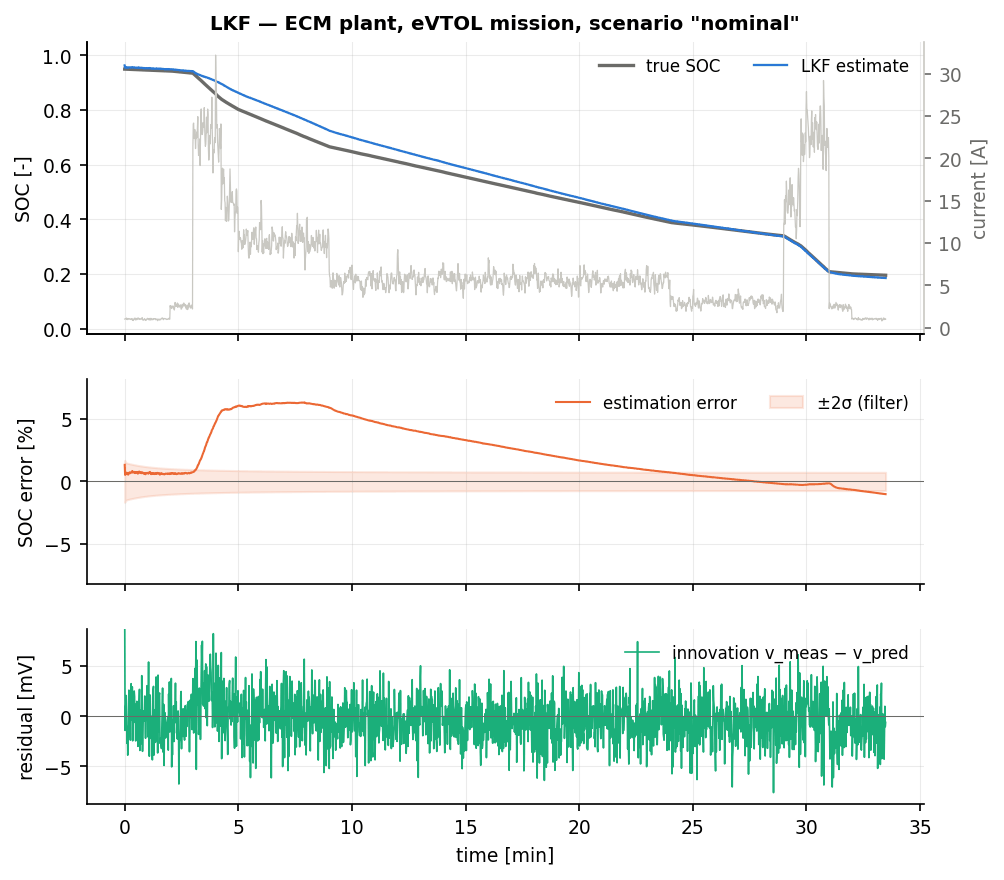
\includegraphics[width=\textwidth]{figures/cell_LKF_nominal.png}
\caption{LKF on the nominal eVTOL mission: true and estimated SOC (top), estimation error with the $\pm 2\sigma$ band when available (middle), voltage residual (bottom).}
\end{figure}
\begin{figure}[H]\centering
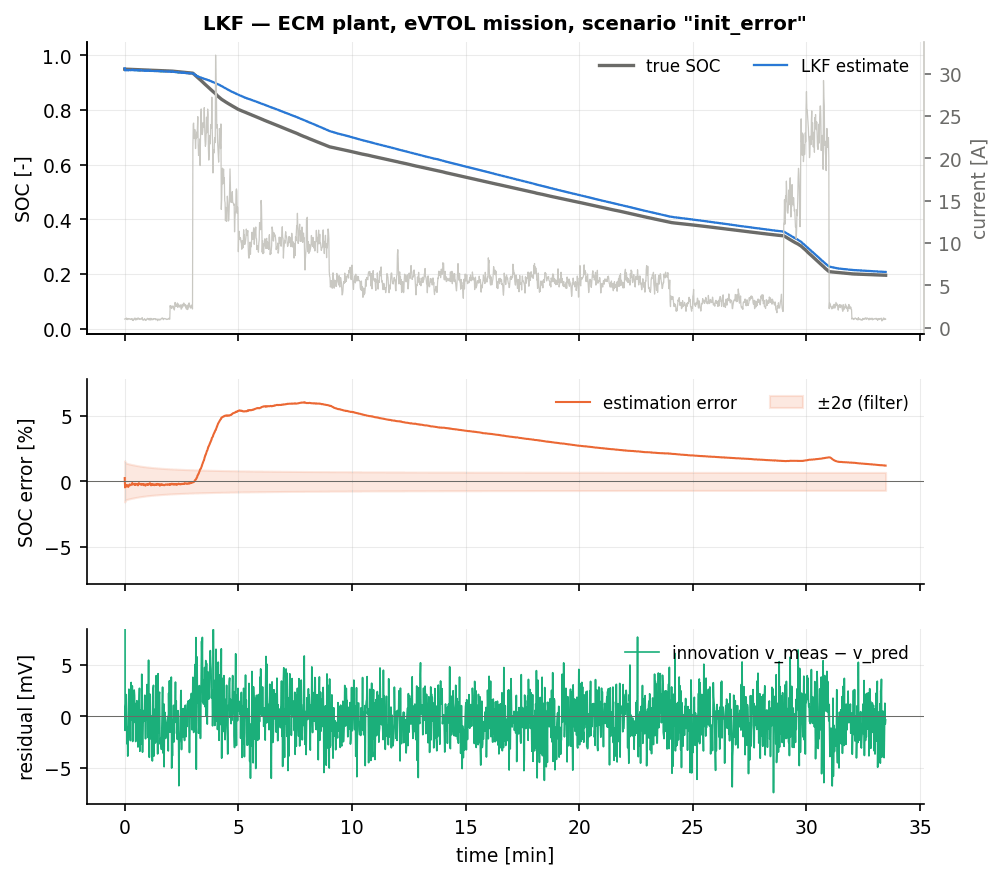
\includegraphics[width=\textwidth]{figures/cell_LKF_init_error.png}
\caption{LKF with a 35\,\% initial SOC error.}
\end{figure}

All numbers are three-seed means in per cent SOC.

The headline number is $\text{RMSE}_{\text{ss}} = 1.19\,\%$ on \texttt{nominal} against the
EKF's $0.05\,\%$: freezing the linearisation costs a factor of twenty-four in steady-state
accuracy, and the whole-run RMSE ($3.23\,\%$ against $0.15\,\%$) a factor of twenty-one. The
filter still converges from the $-35\,\%$ initial error in a single sample, because the gain
computed from $\mP_0$ is large and the frozen $\mH$ has the right sign and roughly the right
magnitude. What it cannot do is track: the error signature in the nominal figure is a slow
drift that follows the deviation of the OCV curve from its tangent, exactly as predicted by
\eqref{eq:lkf-bias}, with a maximum error of $6.29\,\%$. The voltage residual RMSE,
$1.13$\,mV against the EKF's $0.79$\,mV, shows the same bias in the measurement channel. Note
that the whole-run RMSE exceeds the acceptance threshold on several scenarios even though the
steady-state figure does not; the LKF is a filter whose transient is its best part.

\texttt{cold} is the clearest failure: $\text{RMSE}_{\text{ss}} = 12.49\,\%$, ten times worse
than nominal and eighty times worse than the EKF's $0.16\,\%$. The cause is not the OCV but the
frozen RC pole. At $T_0 = 263$\,K the model gives $\tau_1 = 19.1$\,s, hence $a_1 = 0.99477$;
the cell self-heats to $\approx 275$\,K during the mission, where the true $a_1 = 0.99147$.
Since the steady-state RC voltage of the frozen model is
$R_1(T)(1-a_1(T))\,i/(1-a_1^{\text{frozen}})$, the ratio
$(1-a_1^{\text{true}})/(1-a_1^{\text{frozen}}) = 1.63$ means $v_1$ is overestimated by
$63\,\%$ --- and at $22$\,A with a cold $R_1 = 23$\,m$\Omega$ that is a $0.3$\,V error in the
predicted terminal voltage, which the filter can only remove by biasing SOC by
$0.3/0.8\approx 0.19$. An EKF evaluates $a_1(T_k)$ every step and does not have this problem
at all.

\texttt{combined} gives $7.00\,\%$ and never converges; \texttt{init\_error} settles at
$2.19\,\%$ (the frozen tangent is taken at $\soc_0 = 0.60$ there, which fits the lower half of
the OCV curve worse than the tangent at $0.95$ fits the upper half); \texttt{hot} $1.62\,\%$.
Everything else sits at the $1.1$--$1.4\,\%$ tangent-line floor, essentially independent of the
scenario --- \texttt{noise\_step}, \texttt{outliers} and \texttt{sensor\_dropout} are all
$1.19$--$1.20\,\%$, i.e. the LKF does not notice them. \texttt{preisach} is $1.06\,\%$ and
now converges in the first sample, where before the plant's hysteresis sign was corrected it
took over $1300$\,s. As on the ECM plant generally, the LKF is \emph{better} than the EKF on
\texttt{aged\_cell} ($1.14\,\%$ against $1.52\,\%$) and \texttt{param\_mismatch} ($1.19\,\%$
against $1.36\,\%$); that is not a property of the method but a consequence of its low fixed
gain, which is also what makes the SPM result below so striking.

\paragraph{SPM plant: structured model error, and why the LKF wins it.}
\begin{figure}[H]\centering
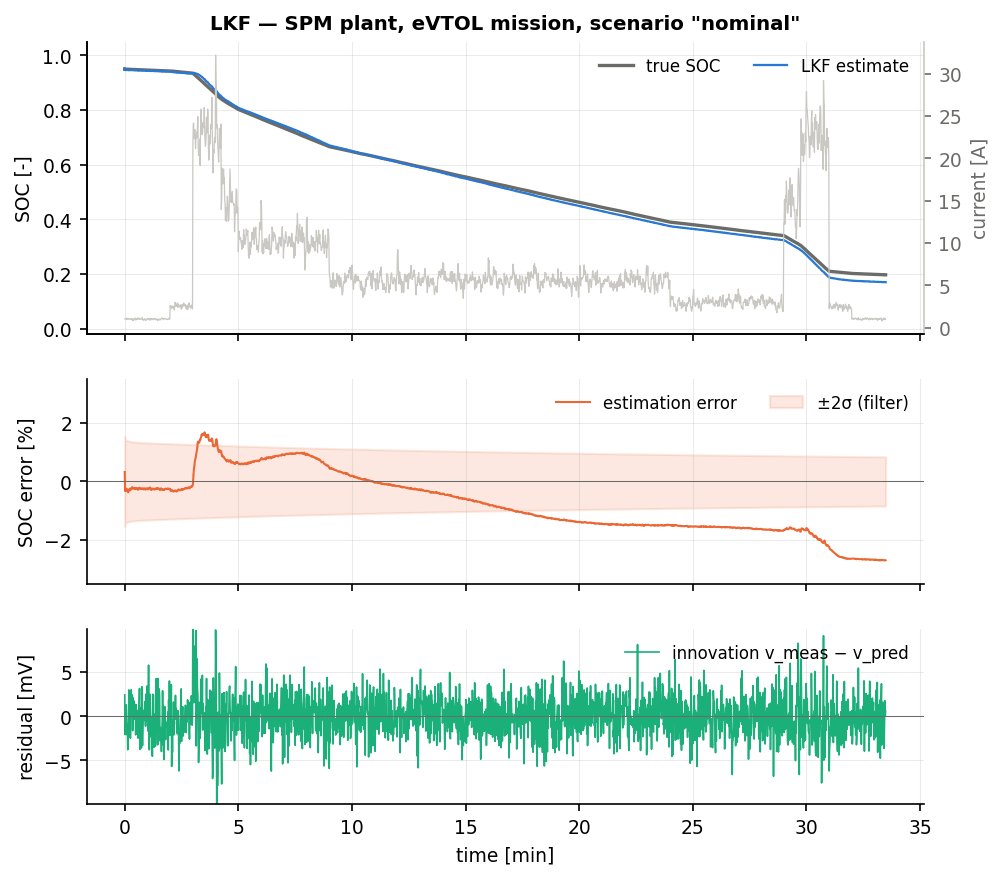
\includegraphics[width=\textwidth]{figures/cellspm_LKF_nominal.png}
\caption{LKF on the nominal mission with the electrochemical (SPM) plant: the frozen gain keeps the estimate close to ampere-hour integration and away from the badly conditioned OCV channel.}
\end{figure}
The SPM block of the table is a different kind of test. The plant is the electrochemical
single-particle model; the estimator still runs a 2-RC equivalent circuit, fitted to that plant,
which leaves a \emph{structured} residual of about $4$\,mV (Butler--Volmer kinetics and
solid-phase diffusion that no 2-RC circuit can reproduce) and a slow second branch,
$\tau_2 = 556$\,s. Over a $33$-minute mission a $556$\,s pole barely relaxes, so $v_2(t)$ is
close to an affine ramp --- and so is $\ocv(\soc(t))$ while the cell discharges at a roughly
constant rate. The two channels through which the measurement sees the state,
$(\partial\ocv/\partial\soc)\,\delta\soc$ and $-\delta v_2$, are therefore nearly collinear in
the information accumulated over the flight: the pair $(\soc, v_2)$ is close to unobservable,
and no filter can decide whether a persistent few-millivolt residual belongs to the slow RC
branch or to the state of charge. Because that direction is weakly observable, a $4$\,mV
structured error maps onto \emph{several per cent} of SOC instead of the
$4\,\text{mV}/0.8\,\text{V}\approx0.5\,\%$ a well-conditioned channel would give. This
$(\soc,v_2)$ ambiguity, not the size of the residual, is the mechanism behind the
$3.7$--$4.6\,\%$ band in which the whole classical family sits.

The LKF is the exception, and by a wide margin: $1.72\,\%$ on SPM \texttt{nominal} against
$3.73\,\%$ for the EKF, $3.96\,\%$ for the UKF and $4.62\,\%$ for the cubature filters, and
$1.47\,\%$ on SPM \texttt{cold} where every other filter in the family is between $7.4$ and
$8.7\,\%$. It is the only member of the family whose SPM performance is no worse than its ECM
performance ($1.72\,\%$ against $1.19\,\%$), and on SPM \texttt{init\_error} it reaches
$0.55\,\%$ --- its best result anywhere in this report.

The explanation is the same rigidity that costs it a factor of twenty on the ECM plant. Its
measurement model is the tangent frozen at $\soc_0$, so it never tracks the OCV slope as the
cell discharges, and the gain along the ill-conditioned $(\soc, v_2)$ direction is fixed once
by the Riccati recursion \eqref{eq:lkf-riccati} rather than re-derived at every step from a
Jacobian that the SPM residual has corrupted. Where an EKF confidently re-linearises and
re-apportions the $4$\,mV residual between $\soc$ and $v_2$ --- committing, step after step, to
a split that the data cannot support --- the LKF simply has no mechanism for doing so. It
therefore stays much closer to open-loop ampere-hour integration, which on the SPM plant is
nearly exact because the current record is clean, and declines to pump the structured residual
into SOC. The $0.55\,\%$ on SPM \texttt{init\_error} is the same effect seen from the other
side: linearising at $\soc_0 = 0.60$ happens to place the frozen tangent where the SPM's true
OCV mapping is best matched.

This is a cautionary result, not a recommendation. The LKF is not modelling the SPM plant
better than the EKF --- it is modelling it worse, and being saved by a low, fixed gain that
keeps it from acting on a corrupted correction. The principled versions of the same idea are a
deliberately de-weighted OCV channel (a larger $\mR$), an $H_\infty$ gain, or an augmented
state that gives the structured residual somewhere to go.

\section{Summary}
The frozen-linearisation Kalman filter is the cheapest member of the family
($320$--$336$\,ns/step, a precomputable gain, no run-time Jacobians) and it converges and
remains stable on every scenario of both plants. It costs a factor of twenty-four in
steady-state SOC accuracy on the nominal ECM mission and fails outright when the operating
point moves far from the linearisation point in \emph{temperature}, because the frozen RC poles
then describe the wrong cell. Its one genuine success is the SPM plant, where its low fixed
gain makes it the most accurate filter of the family under structured model error --- for the
wrong reason. Use it only where the SOC window and the temperature are both narrow and a
$1$--$2\,\%$ SOC error is acceptable; for anything resembling a full discharge, re-linearising
every step costs $140$\,ns more and is twenty times more accurate.

% Copyright 2026 Sreeram Anil
% SPDX-License-Identifier: CC-BY-4.0
% =============================================================================
%  Iterated extended Kalman filter — classical Kalman family
% =============================================================================
\chapter{Iterated Extended Kalman Filter (IEKF)}
\label{ch:iekf}

\section*{At a glance}
\begin{tabular}{@{}l>{\raggedright\arraybackslash}p{0.76\textwidth}@{}}
Family & classical Kalman \\
Header & \texttt{include/estkit/filters/iekf.hpp} \\
Registered name & \texttt{IEKF} \\
State dimension & $n_x = 4$ (cell model) --- generic in $n_x, n_u, n_y$ \\
Cost per step & $\mathcal{O}(J n_x^3)$, $J\le5$ iterations; $0.56$--$0.60\,\SI{}{\micro\second}$/step \\
Primary references & \cite{jazwinski1970,bellcathey1993,gelb1974} \\
\end{tabular}

\section{Motivation and aerospace/BMS relevance}
The EKF linearises the measurement function at the \emph{prior} mean $\xminus$. That is the
only point available before the measurement arrives, but it is the wrong point: after the
update the state is somewhere else, and if the innovation is large the Jacobian used to
compute the gain describes the wrong part of the nonlinearity. The classical cure, already in
Jazwinski's 1970 book~\cite[\S8.3]{jazwinski1970}, is to iterate --- relinearise at the
updated estimate and repeat the update until it stops moving.

Bell and Cathey~\cite{bellcathey1993} identified the recursion as Gauss--Newton applied to
the maximum-a-posteriori cost, which turned a heuristic into an optimisation algorithm with
known convergence behaviour and made it clear what the filter is actually computing: the
posterior \emph{mode} rather than a one-step linear approximation of the mean.

In BMS terms the relevant situation is a large voltage innovation: first power-up with an
unknown SOC, recovery after a sensor dropout, or a step change in load that the model gets
wrong. The OCV curve of an NMC/graphite cell is markedly nonlinear near the ends of the SOC
window, so a $0.3$\,V innovation corresponds to very different SOC corrections depending on
where the tangent is taken. In GNC the same argument is made for angles-only navigation and
for terrain-relative navigation, where a single measurement can carry a large correction.

\section{Problem statement and assumptions}
Model \eqref{eq:ekf-proc}--\eqref{eq:ekf-meas}. The time update is the EKF's. For the
measurement update, given the prior $\xminus_k$, $\Pminus_k$ and the observation $\vy_k$,
consider the maximum-a-posteriori (MAP) problem
\begin{equation}
\xplus_k = \argmin_{\vx}\; J(\vx), \qquad
J(\vx) = \tfrac12\norm{\vx - \xminus_k}^2_{(\Pminus_k)\inv} + \tfrac12\norm{\vy_k - h(\vx,\vu_k)}^2_{\mR\inv},
\label{eq:iekf-map}
\end{equation}
where $\norm{\bm{a}}^2_{\bm{M}} := \bm{a}^\T\bm{M}\bm{a}$. If $h$ were affine, $J$ would be a
quadratic whose minimiser is the EKF update; in general \eqref{eq:iekf-map} must be solved
iteratively. The assumption is that $h$ is twice differentiable and that $J$ has a unique
local minimum in the region of interest.

\section{Derivation}
Apply Gauss--Newton to \eqref{eq:iekf-map}. Writing $\mH_j = \partial h/\partial\vx|_{\vx_j}$
and linearising the residual $\vy_k - h(\vx,\vu_k)$ about the current iterate $\vx_j$,
\begin{equation}
J(\vx) \approx \tfrac12\norm{\vx-\xminus_k}^2_{(\Pminus_k)\inv}
 + \tfrac12\norm{\vy_k - h(\vx_j,\vu_k) - \mH_j(\vx-\vx_j)}^2_{\mR\inv}.
\label{eq:iekf-quad}
\end{equation}
Setting the gradient of \eqref{eq:iekf-quad} to zero and using the matrix inversion lemma to
turn the information-form solution into a gain form gives the iteration
\begin{align}
\mK_j &= \Pminus_k\mH_j^\T\left(\mH_j\Pminus_k\mH_j^\T + \mR\right)\inv, \label{eq:iekf-K}\\
\vx_{j+1} &= \xminus_k + \mK_j\left[\vy_k - h(\vx_j,\vu_k) - \mH_j\left(\xminus_k - \vx_j\right)\right],
\qquad \vx_0 = \xminus_k. \label{eq:iekf-iter}
\end{align}
The bracketed quantity is the residual that the linearised measurement predicts \emph{at the
prior mean}: for $j=0$ it reduces to the ordinary innovation $\vy_k - h(\xminus_k,\vu_k)$, so
\textbf{one iteration reproduces the EKF exactly}. The correction term
$-\mH_j(\xminus_k - \vx_j)$ is what keeps the prior anchored at $\xminus_k$ while the
expansion point moves.

Bell and Cathey~\cite{bellcathey1993} show that \eqref{eq:iekf-iter} is precisely the
Gauss--Newton step for \eqref{eq:iekf-map} with the Gauss--Newton Hessian approximation
$\nabla^2 J \approx (\Pminus_k)\inv + \mH^\T\mR\inv\mH$, hence: (i) it converges locally at a
rate governed by the residual size times the curvature (quadratic for zero-residual
problems), (ii) it may diverge for large residuals, which is why a damping factor
$\theta\in(0,1]$, $\vx_{j+1} = \vx_j + \theta\,\Delta_j$, is retained as an option, and
(iii) the natural covariance is the inverse Gauss--Newton Hessian evaluated at the solution,
\begin{equation}
\Pplus_k = \left[(\Pminus_k)\inv + \mH_J^\T\mR\inv\mH_J\right]\inv
 = (\mI - \mK_J\mH_J)\Pminus_k,
\label{eq:iekf-cov}
\end{equation}
implemented in Joseph form. The implementation uses the $(\mH_J,\mK_J)$ of the last executed
step, which makes the $J=1$ case bit-identical to the EKF (verified: max
$\abs{\Delta\vx}=0$, max $\abs{\Delta\mP}=0$ over a full mission) and is immaterial at
convergence, where $\mH_{J-1}=\mH_J$ to working precision.

\begin{remark}[What the IEKF does \emph{not} fix]
The iteration improves the \emph{location} of the linearisation, not the \emph{spread}: the
innovation covariance $\mH_j\Pminus\mH_j^\T+\mR$ is still a first-order quantity and still
ignores the variance injected by the curvature of $h$. The IEKF is therefore as
over-confident as the EKF; only the second-order filter (Chapter~\ref{ch:soekf}) and the
sigma-point statistical-linearisation filters (Chapters~\ref{ch:ukf},~\ref{ch:iplf}) repair
that.
\end{remark}

\section{Algorithm}
\begin{algorithm}[H]
\caption{IEKF --- one sampling period}
\begin{algorithmic}[1]
\Require $\xplus_{k-1},\Pplus_{k-1},\vu_{k-1},\vy_k,\vu_k$, $J_{\max}$, tolerance $\epsilon$, damping $\theta$
\State \textbf{Time update:} as the EKF, \eqref{eq:ekf-tu-mean}--\eqref{eq:ekf-tu-cov}
\State $\vx_0 \gets \xminus_k$
\For{$j = 0,\dots,J_{\max}-1$}
  \State $\mH_j \gets \partial h/\partial\vx|_{\vx_j,\vu_k}$; \;
         $\mS_j \gets \mH_j\Pminus_k\mH_j^\T+\mR$; \;
         $\mK_j \gets \Pminus_k\mH_j^\T\mS_j\inv$
  \State $\Delta \gets \theta\left[\xminus_k + \mK_j\left(\vy_k - h(\vx_j,\vu_k) - \mH_j(\xminus_k-\vx_j)\right) - \vx_j\right]$
  \State $\vx_{j+1}\gets\vx_j+\Delta$
  \State \textbf{if} $\norm{\Delta}\le\epsilon(1+\norm{\vx_{j+1}})$ \textbf{then break}
\EndFor
\State $\xplus_k \gets \vx_{J}$; \;
       $\Pplus_k \gets (\mI-\mK_{J-1}\mH_{J-1})\Pminus_k(\cdot)^\T + \mK_{J-1}\mR\mK_{J-1}^\T$
\State \textbf{if} constraints enabled \textbf{then} $\xplus_k\gets\Pi(\xplus_k)$
\Ensure $\xplus_k,\Pplus_k$
\end{algorithmic}
\end{algorithm}

\section{Application to the battery model}
Only one entry of $\mH$ depends on the state, $\mH_1 = \partial\ocv/\partial\soc(\soc,T)$, so
the Gauss--Newton iteration is effectively a scalar Newton solve for the SOC that satisfies
the voltage equation. Because the estimator-side OCV is a $241$-point piecewise-linear table,
$\mH_1$ is piecewise constant in $\soc$: the iteration converges in one or two steps whenever
successive iterates stay inside the same table segment, and can oscillate between two
adjacent segments otherwise --- which is why a finite $J_{\max}$ and a relative tolerance are
both needed, rather than ``iterate to convergence''.

Benchmark options: \code{max\_iter = 5}, \code{tol = }$10^{-6}$, \code{step = 1} (no
damping), \code{joseph = true}, \code{apply\_constraints = true}. Five iterations is the
value used in most of the literature and is what the assignment prescribes; measurements of
the sensitivity are reported below.

\section{Implementation notes}
Each iteration costs one Jacobian evaluation, one $n_y\times n_y$ inverse and two
$n_x\times n_y$ products; the covariance update is done once, outside the loop. The loop exits
early on $\norm{\Delta}\le\epsilon(1+\norm{\vx})$, and the measured cost
($0.56$--$0.60\,\SI{}{\micro\second}$/step against the EKF's $0.44$--$0.48$) shows that the
loop usually terminates after two passes in steady state. There is no extra memory:
\code{sizeof(Iekf<EcmModel>)} equals \code{sizeof(Ekf<EcmModel>)} at 4336\,bytes.
Guards: the loop breaks if the gain or the step is not finite, and the covariance update is
skipped if $\mK$ is not finite, so a singular $\mS$ leaves the prior untouched rather than
producing NaN.

\section{Benchmark results}
% Copyright 2026 Sreeram Anil
% SPDX-License-Identifier: CC-BY-4.0
\begin{table}[H]\centering\footnotesize\setlength{\tabcolsep}{4pt}
\caption{IEKF: cell-level benchmark on the eVTOL mission (mean over seeds; RMSE and max error in \% SOC; $t_\mathrm{conv}$: first time the error stays below 2\,\% for 60\,s, -- = never; EKF reference: steady-state RMSE of the plain EKF on the same data).}\label{tab:cell_IEKF}
\begin{tabular}{llrrrrrcrr}\toprule
plant & scenario & RMSE & RMSE$_\mathrm{ss}$ & max & $t_\mathrm{conv}$ [s] & RMSE$_v$ [mV] & div. & EKF ref. & ns/step \\ \midrule
ECM & nominal & 0.30 & 0.08 & 1.15 & 0 & 0.79 & no & 0.05 & 596 \\
ECM & init\_error & 0.18 & 0.06 & 0.88 & 0 & 2.12 & no & 0.05 & 594 \\
ECM & current\_bias & 0.61 & 0.64 & 1.47 & 0 & 0.86 & no & 0.61 & 600 \\
ECM & noise\_step & 0.37 & 0.27 & 1.15 & 0 & 2.89 & no & 0.12 & 596 \\
ECM & outliers & 1.06 & 0.36 & 6.27 & 242 & 2.09 & no & 0.21 & 596 \\
ECM & cold & 0.34 & 0.15 & 1.27 & 0 & 1.90 & no & 0.16 & 593 \\
ECM & hot & 0.17 & 0.03 & 0.90 & 0 & 0.54 & no & 0.03 & 599 \\
ECM & aged\_cell & 1.31 & 1.69 & 4.04 & 0 & 3.82 & no & 1.52 & 597 \\
ECM & param\_mismatch & 1.43 & 1.50 & 3.06 & 0 & 2.81 & no & 1.36 & 599 \\
ECM & sensor\_dropout & 0.37 & 0.19 & 1.29 & 0 & 1.72 & no & 0.46 & 594 \\
ECM & preisach & 0.91 & 0.21 & 2.95 & 153 & 0.82 & no & 0.20 & 594 \\
ECM & combined & 1.84 & 2.13 & 4.22 & 0 & 4.58 & no & 12.44 & 603 \\
\midrule
SPM & nominal & 3.55 & 3.66 & 4.12 & 0 & 1.02 & no & 3.73 & 568 \\
SPM & init\_error & 3.04 & 3.13 & 3.58 & 0 & 2.18 & no & 3.81 & 567 \\
SPM & current\_bias & 4.89 & 5.67 & 6.52 & 0 & 1.12 & no & 5.69 & 569 \\
SPM & noise\_step & 3.77 & 4.05 & 4.84 & 0 & 3.14 & no & 3.30 & 577 \\
SPM & outliers & 2.02 & 1.73 & 6.46 & 150 & 2.31 & no & 1.99 & 555 \\
SPM & cold & 7.27 & 7.49 & 9.16 & -- & 4.33 & no & 7.35 & 560 \\
SPM & hot & 2.05 & 2.12 & 2.38 & 0 & 0.69 & no & 2.16 & 567 \\
SPM & param\_mismatch & 2.59 & 2.87 & 3.50 & 0 & 1.96 & no & 3.13 & 568 \\
SPM & sensor\_dropout & 5.01 & 5.18 & 5.85 & 0 & 1.95 & no & 5.31 & 569 \\
\bottomrule\end{tabular}\end{table}

\begin{figure}[H]\centering
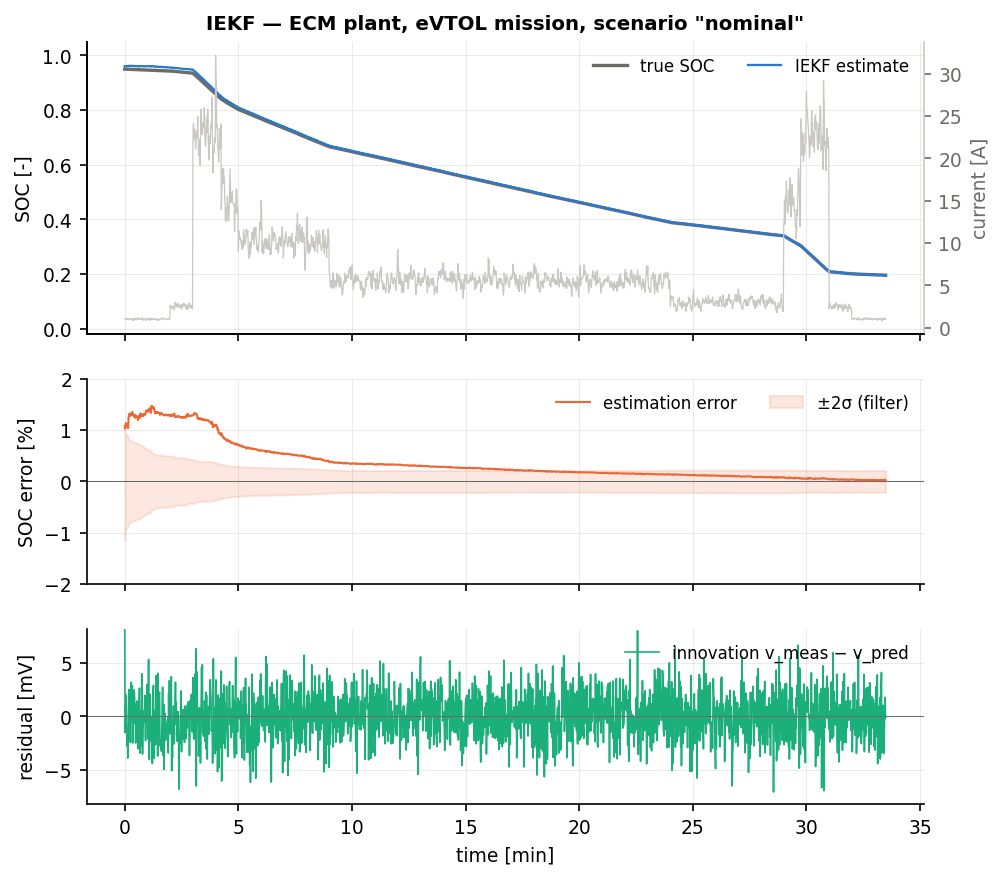
\includegraphics[width=\textwidth]{figures/cell_IEKF_nominal.png}
\caption{IEKF on the nominal eVTOL mission: true and estimated SOC (top), estimation error with the $\pm 2\sigma$ band when available (middle), voltage residual (bottom).}
\end{figure}
\begin{figure}[H]\centering
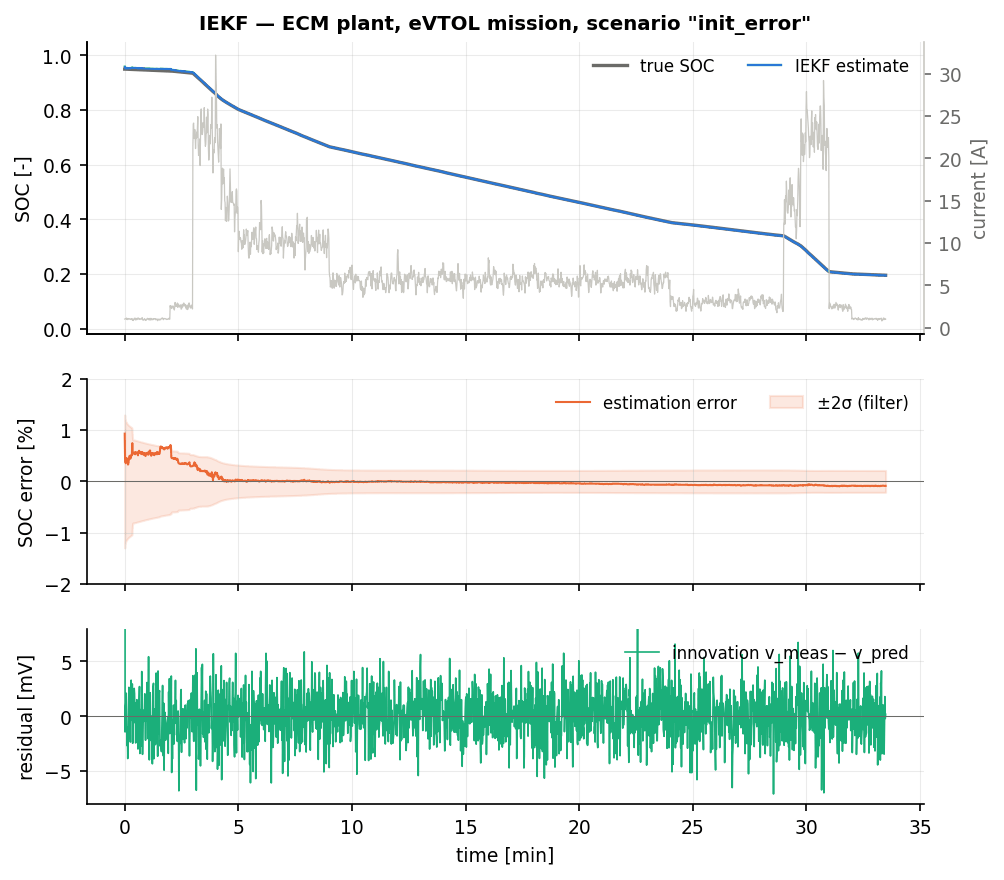
\includegraphics[width=\textwidth]{figures/cell_IEKF_init_error.png}
\caption{IEKF with a 35\,\% initial SOC error.}
\end{figure}

All numbers are three-seed means in per cent SOC.

On \texttt{nominal} the IEKF gives $\text{RMSE} = 0.30\,\%$, $\text{RMSE}_{\text{ss}} =
0.08\,\%$, against the EKF's $0.15/0.05\,\%$ --- slightly \emph{worse}. That is not a
contradiction: in nominal operation the innovations are at the millivolt level, the expansion
point barely moves, and the extra iterations only shuffle the correction between $\soc$ and the
RC and hysteresis states. The voltage-residual RMSE is identical to the EKF's
($0.79$\,mV for both), confirming that the two filters fit the measurement equally well and
differ only in how they distribute the correction.

Where a large innovation really occurs the iteration earns its keep. On \texttt{combined} the
EKF never converges ($12.44\,\%$) while the IEKF converges in the first sample and reaches
$2.13\,\%$ --- a factor of six better, obtained purely by relinearising, and the best maximum
error of the whole family on that scenario ($4.22\,\%$ against the EKF's $29.6\,\%$). On
\texttt{sensor\_dropout} ($15$\,s of stuck voltage) the IEKF gives $0.19\,\%$ against the EKF's
$0.46\,\%$ and the UKF's $0.86\,\%$, second only to the second-order EKF's $0.18\,\%$: after
the fault clears the
innovation is large and the first Gauss--Newton step is the wrong one, but the second and third
recover. \texttt{cold} improves slightly ($0.15\,\%$ against $0.16\,\%$) and \texttt{hot} is
unchanged at $0.03\,\%$.

The counter-example is \texttt{outliers} ($5\,\%$ of samples corrupted by $\pm 50$\,mV), where
the IEKF degrades to $0.36\,\%$ against the EKF's $0.21\,\%$ and the convergence metric is
pushed out to $242$\,s against $16$\,s. The reason is structural and worth stating plainly:
Gauss--Newton makes the filter fit the current measurement \emph{better}, and an outlier is a
measurement that must not be fitted at all. Iterating a least-squares update is the opposite of
robust estimation; when outliers are expected, the iteration must be combined with a robust
loss (Huber, Student-$t$) rather than used alone. \texttt{aged\_cell} ($1.69\,\%$ against
$1.52\,\%$) and \texttt{param\_mismatch} ($1.50\,\%$ against $1.36\,\%$) show a milder version
of the same effect: a better fit to a biased model is still biased.

Sensitivity to $J_{\max}$ was measured during development on four scenarios: $J = 1$ reproduces
the EKF exactly, $J = 2$ gives the best \texttt{combined} result, and $J = 3, 5, 10$ are
non-monotone. That non-monotonicity is a reminder that the iteration is solving the
\emph{wrong} problem slightly better: the MAP estimate of a model that is itself biased by an
unmodelled $25\,\%$ increase in $R_0$.

\paragraph{SPM plant: structured model error.}
\begin{figure}[H]\centering
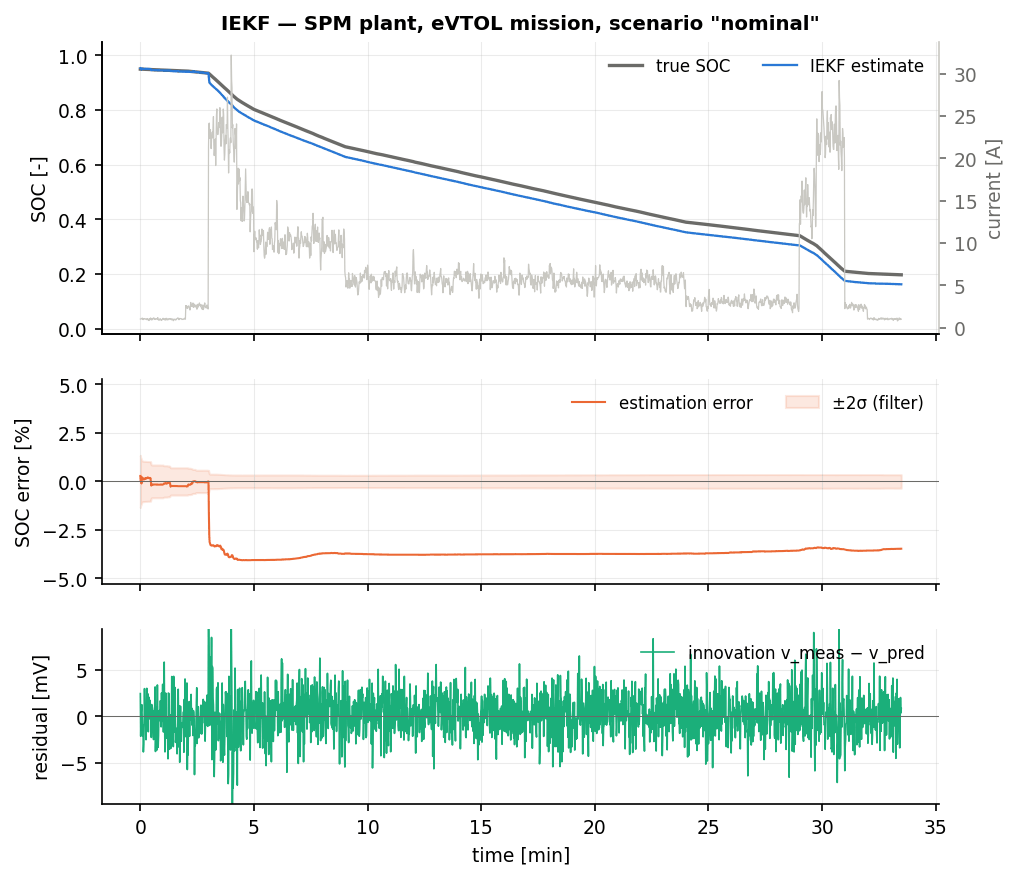
\includegraphics[width=\textwidth]{figures/cellspm_IEKF_nominal.png}
\caption{IEKF on the nominal mission with the electrochemical (SPM) plant.}
\end{figure}
The SPM block of the table is a different kind of test. The plant is the electrochemical
single-particle model; the estimator still runs a 2-RC equivalent circuit, fitted to that plant,
which leaves a \emph{structured} residual of about $4$\,mV (Butler--Volmer kinetics and
solid-phase diffusion that no 2-RC circuit can reproduce) and a slow second branch,
$\tau_2 = 556$\,s. Over a $33$-minute mission a $556$\,s pole barely relaxes, so $v_2(t)$ is
close to an affine ramp --- and so is $\ocv(\soc(t))$ while the cell discharges at a roughly
constant rate. The two channels through which the measurement sees the state,
$(\partial\ocv/\partial\soc)\,\delta\soc$ and $-\delta v_2$, are therefore nearly collinear in
the information accumulated over the flight: the pair $(\soc, v_2)$ is close to unobservable,
and no filter can decide whether a persistent few-millivolt residual belongs to the slow RC
branch or to the state of charge. Because that direction is weakly observable, a $4$\,mV
structured error maps onto \emph{several per cent} of SOC instead of the
$4\,\text{mV}/0.8\,\text{V}\approx0.5\,\%$ a well-conditioned channel would give. This
$(\soc,v_2)$ ambiguity, not the size of the residual, is the mechanism behind the
$3.7$--$4.6\,\%$ band in which the whole classical family sits.

The IEKF is marginally the best of the first-order Taylor-linearising filters here: $3.66\,\%$ on SPM
\texttt{nominal} against the EKF's $3.73\,\%$, $3.13\,\%$ on \texttt{init\_error} against
$3.81\,\%$, $2.87\,\%$ on \texttt{param\_mismatch} against $3.13\,\%$, $5.18\,\%$ on
\texttt{sensor\_dropout} against $5.31\,\%$. The improvements are real but small, and they are
of the same size as the improvement iterating buys on the ECM plant when the innovation is
large. What the iteration cannot do is resolve the ambiguity: relinearising more accurately at
the posterior does not add information along a direction in which the measurement carries
none, so the IEKF remains squarely inside the $3.7$--$4.6\,\%$ band. \texttt{cold} is in fact
slightly worse than the EKF's ($7.49\,\%$ against $7.35\,\%$), for the same reason
\texttt{outliers} was worse on the ECM plant: a tighter fit to a structurally wrong measurement
is not an improvement.

\section{Summary}
The IEKF costs one to four extra Jacobian evaluations per step
($0.56$--$0.60\,\SI{}{\micro\second}$ against the EKF's $0.44$--$0.48$) and converts the EKF's
one-shot linear update into a Gauss--Newton solve for the posterior mode. Use it when large
innovations are expected --- initialisation, post-fault recovery, sparse or infrequent
measurements --- and when the measurement function is strongly curved in the observed
direction; on this benchmark it turns the EKF's worst failure (\texttt{combined}, factor of
six) and its worst fault scenario (\texttt{sensor\_dropout}, factor of two) into good results.
Do not use it when the measurement stream contains outliers, because iterating fits them
harder, and do not expect it to fix over-confidence or structured model error: the covariance
is still first order and the SPM rows are within $2\,\%$ of the plain EKF's.

% Copyright 2026 Sreeram Anil
% SPDX-License-Identifier: CC-BY-4.0
% =============================================================================
%  Second-order extended Kalman filter — classical Kalman family
% =============================================================================
\chapter{Second-Order Extended Kalman Filter (SO-EKF)}
\label{ch:soekf}

\section*{At a glance}
\begin{tabular}{@{}l>{\raggedright\arraybackslash}p{0.76\textwidth}@{}}
Family & classical Kalman \\
Header & \texttt{include/estkit/filters/soekf.hpp} \\
Registered name & \texttt{SO-EKF} \\
State dimension & $n_x = 4$ (cell model) --- generic in $n_x, n_u, n_y$ \\
Cost per step & $\mathcal{O}(n_x^4)$ traces, $2n_x(n_x{+}1)$ model calls per Hessian; $3.9$--$4.2\,\SI{}{\micro\second}$/step \\
Primary references & \cite{athans1968,jazwinski1970,bass1966,maybeck1982vol2,gelb1974} \\
\end{tabular}

\section{Motivation and aerospace/BMS relevance}
The EKF truncates the Taylor expansion of $f$ and $h$ after the linear term. The next term is
not small when the state uncertainty is large: for a scalar function $\phi$ and
$\vx\sim\N{\xhat}{\mP}$,
\begin{equation}
\E{\phi(\vx)} = \phi(\xhat) + \tfrac12\tr\!\left(\nabla^2\phi(\xhat)\,\mP\right) + \mathcal{O}(\mP^2),
\label{eq:soekf-motivation}
\end{equation}
so the EKF's predicted measurement is biased by $\tfrac12\tr(\nabla^2h\,\mP)$ and its
innovation covariance is too small by a term of the same order squared. Athans, Wishner and
Bertolini~\cite{athans1968} derived the filter that keeps these terms --- the ``modified
truncated second-order filter'' --- and demonstrated on a scalar nonlinear example that it
removes a bias the EKF cannot see. Jazwinski~\cite[Ch.~9]{jazwinski1970} and
Bass, Norum and Schwartz~\cite{bass1966} give the general Gaussian second-order form.

For SOC estimation this term has a concrete meaning: it is the curvature of the OCV
characteristic. When $\sigma_\soc$ is at its start-up value of $0.1$, the average of
$\ocv(\soc)$ over the prior differs from $\ocv(\hat{\soc})$ by tens of millivolts --- more
than ten times the voltage-sensor noise --- and the true variance of the predicted voltage is
substantially larger than $\mH\mP\mH^\T+\mR$. An EKF that ignores both becomes confident too
early and locks in whatever error it made on the first update. This chapter shows that
correcting it explicitly is the single most effective change made to the EKF in this family.

\section{Problem statement and assumptions}
Model \eqref{eq:ekf-proc}--\eqref{eq:ekf-meas}. $f$ and $h$ are assumed twice continuously
differentiable, and the conditional density is assumed Gaussian so that the third central
moment vanishes and the fourth factorises (Isserlis' theorem) --- these are exactly the
assumptions that make the trace formulae below exact to the stated order. Write
$\nabla^2 f_i$ and $\nabla^2 h_i$ for the $n_x\times n_x$ Hessians of the $i$-th components
of $f$ and $h$.

\section{Derivation}
\paragraph{Mean correction.} Expanding $f_i$ to second order about $\xplus_{k-1}$ with
$\bm{e} = \vx - \xplus_{k-1}$, $\E{\bm e}=\bm0$, $\E{\bm e\bm e^\T}=\Pplus_{k-1}$:
\begin{equation}
\E{f_i(\vx)} = f_i(\xplus_{k-1}) + \underbrace{\E{\nabla f_i^\T\bm e}}_{=0}
 + \tfrac12\E{\bm e^\T\nabla^2f_i\,\bm e} + \dots
 = f_i(\xplus_{k-1}) + \tfrac12\tr\!\left(\nabla^2f_i\,\Pplus_{k-1}\right) + \dots
\label{eq:soekf-mean}
\end{equation}
using $\E{\bm e^\T\mA\bm e} = \tr(\mA\,\E{\bm e\bm e^\T})$.

\paragraph{Covariance correction.} For the $(i,j)$ entry, keeping terms up to second order in
$\mP$ and using the Gaussian fourth-moment identity
$\E{\bm e^\T\mA\bm e\,\bm e^\T\mB\bm e} = \tr(\mA\mP)\tr(\mB\mP) + 2\tr(\mA\mP\mB\mP)$,
\begin{equation}
\left(\operatorname{Cov}[f(\vx)]\right)_{ij}
= \left(\mF\mP\mF^\T\right)_{ij} + \tfrac12\tr\!\left(\nabla^2f_i\,\mP\,\nabla^2f_j\,\mP\right) + \dots
\label{eq:soekf-cov}
\end{equation}
(the $\tr(\mA\mP)\tr(\mB\mP)$ part is cancelled exactly by the mean correction
\eqref{eq:soekf-mean}, which is why the mean and covariance corrections must be applied
together). The same two formulae applied to $h$ give the corrected predicted measurement and
innovation covariance. Collecting:
\begin{align}
\xminus_k &= f(\xplus_{k-1},\vu_{k-1}) + \tfrac12\sum_i \bm{e}_i\,\tr\!\left(\nabla^2f_i\,\Pplus_{k-1}\right),
\label{eq:soekf-tu-mean}\\
\Pminus_k &= \mF\Pplus_{k-1}\mF^\T + \mQ
 + \tfrac12\left[\tr\!\left(\nabla^2f_i\,\Pplus_{k-1}\nabla^2f_j\,\Pplus_{k-1}\right)\right]_{ij},
\label{eq:soekf-tu-cov}\\
\yhat_k &= h(\xminus_k,\vu_k) + \tfrac12\sum_i \bm{e}_i\,\tr\!\left(\nabla^2h_i\,\Pminus_k\right),
\label{eq:soekf-ymean}\\
\tilde{\mR}_k &= \mR + \tfrac12\left[\tr\!\left(\nabla^2h_i\,\Pminus_k\nabla^2h_j\,\Pminus_k\right)\right]_{ij},
\qquad \mS_k = \mH\Pminus_k\mH^\T + \tilde{\mR}_k,
\label{eq:soekf-S}
\end{align}
with $\bm e_i$ the $i$-th unit vector. The gain and the state update are the EKF's,
$\mK_k = \Pminus_k\mH^\T\mS_k\inv$, $\xplus_k = \xminus_k + \mK_k(\vy_k-\yhat_k)$.

\begin{proposition}[Joseph form remains exact]\label{prop:soekf-joseph}
With $\mK_k = \Pminus_k\mH^\T\mS_k\inv$ and $\mS_k$ as in \eqref{eq:soekf-S},
\begin{equation}
(\mI-\mK_k\mH)\Pminus_k(\mI-\mK_k\mH)^\T + \mK_k\tilde{\mR}_k\mK_k^\T
= \Pminus_k - \mK_k\mS_k\mK_k^\T .
\label{eq:soekf-joseph}
\end{equation}
\end{proposition}
\begin{proof}
Expanding the left side gives
$\Pminus - \mK\mH\Pminus - \Pminus\mH^\T\mK^\T + \mK(\mH\Pminus\mH^\T+\tilde{\mR})\mK^\T
= \Pminus - \mK\mH\Pminus - \Pminus\mH^\T\mK^\T + \mK\mS\mK^\T$. Since
$\mK\mS\mK^\T = \Pminus\mH^\T\mS\inv\mH\Pminus = \mK\mH\Pminus = \Pminus\mH^\T\mK^\T$, this
equals $\Pminus - \mK\mS\mK^\T$.
\end{proof}
Proposition~\ref{prop:soekf-joseph} means the numerically preferable Joseph form can be used
unchanged provided $\mR$ is replaced by the inflated $\tilde{\mR}$ --- a point that is easy to
get wrong in implementations.

\paragraph{Numerical Hessians.} The model concept exposes $f$, $h$ and (optionally) their
Jacobians, never second derivatives, so the Hessians are built by central differences:
\begin{equation}
\left(\nabla^2 g_c\right)_{ab} \approx
\frac{g_c(\vx{+}h_a\bm e_a{+}h_b\bm e_b) - g_c(\vx{+}h_a\bm e_a{-}h_b\bm e_b)
 - g_c(\vx{-}h_a\bm e_a{+}h_b\bm e_b) + g_c(\vx{-}h_a\bm e_a{-}h_b\bm e_b)}{4h_ah_b},
\label{eq:soekf-hess}
\end{equation}
with $h_a = \rho(1+\abs{x_a})$. For $a=b$ this degenerates to the usual
$[g(\vx{+}2h)-2g(\vx)+g(\vx{-}2h)]/(4h^2)$. One sweep produces all $n_y$ (or $n_x$) component
Hessians simultaneously, costing $2n_x(n_x{+}1) = 40$ evaluations of the model for $n_x = 4$.

\section{Algorithm}
\begin{algorithm}[H]
\caption{SO-EKF --- one sampling period}
\begin{algorithmic}[1]
\Require $\xplus_{k-1},\Pplus_{k-1},\vu_{k-1},\vy_k,\vu_k$, Hessian step $\rho$
\State \textbf{Time update:} $\mF\gets\partial f/\partial\vx$;\;
       $\{\nabla^2f_i\}\gets$ central differences \eqref{eq:soekf-hess}
\State $\xminus_k\gets f(\xplus_{k-1},\vu_{k-1})+\tfrac12\sum_i\bm e_i\tr(\nabla^2f_i\Pplus_{k-1})$
\State $\Pminus_k\gets\mF\Pplus_{k-1}\mF^\T+\mQ+\tfrac12[\tr(\nabla^2f_i\Pplus\nabla^2f_j\Pplus)]_{ij}$; symmetrise
\State \textbf{Predicted measurement:} $\{\nabla^2h_i\}\gets$ central differences at $\xminus_k$ (cached)
\State $\yhat_k\gets h(\xminus_k,\vu_k)+\tfrac12\sum_i\bm e_i\tr(\nabla^2h_i\Pminus_k)$
\State \textbf{Measurement update:}
       $\tilde{\mR}\gets\mR+\tfrac12[\tr(\nabla^2h_i\Pminus\nabla^2h_j\Pminus)]_{ij}$;\;
       $\mS\gets\mH\Pminus_k\mH^\T+\tilde{\mR}$
\State $\mK\gets\Pminus_k\mH^\T\mS\inv$;\; $\xplus_k\gets\xminus_k+\mK(\vy_k-\yhat_k)$
\State $\Pplus_k\gets(\mI-\mK\mH)\Pminus_k(\mI-\mK\mH)^\T+\mK\tilde{\mR}\mK^\T$; symmetrise
\State \textbf{if} constraints enabled \textbf{then} $\xplus_k\gets\Pi(\xplus_k)$
\Ensure $\xplus_k,\Pplus_k$
\end{algorithmic}
\end{algorithm}

\section{Application to the battery model}
The cell dynamics are affine in $\vx$, so $\nabla^2 f_i \equiv \bm0$ and the entire
second-order content sits in the measurement equation, where the only non-zero Hessian entry
is $\partial^2\ocv/\partial\soc^2$ (the $\mH$ entries for $v_1,v_2,h$ are constants). The
mean correction is therefore
\begin{equation}
\yhat_k = h(\xminus_k,\vu_k) + \tfrac12\,\ocv''(\soc)\,\sigma_\soc^2,
\qquad
\tilde{R} = R + \tfrac12\left(\ocv''(\soc)\,\sigma_\soc^2\right)^2 ,
\label{eq:soekf-battery}
\end{equation}
which at start-up ($\sigma_\soc = 0.1$, $\ocv''\approx -6$\,V) is a $-30$\,mV bias correction
and adds $1.8\times10^{-3}$\,V$^2$ to an innovation variance of $5.6\times10^{-3}$\,V$^2$
(a $32\,\%$ inflation, against a sensor term $\mR = 4.4\times10^{-6}$\,V$^2$ that is four
hundred times smaller), and in steady state
($\sigma_\soc\approx10^{-3}$) is $3\,\SI{}{\micro\volt}$ and nothing. The filter therefore
degrades gracefully to the EKF exactly when the EKF is right.

\paragraph{Choice of the differencing step.} This is the one real implementation decision.
The theoretically optimal relative step for a second derivative in double precision is
$\varepsilon^{1/4}\approx 1.2\times10^{-4}$, which balances round-off against truncation for a
\emph{smooth} function. The estimator-side OCV, however, is a $241$-point piecewise-linear
table with spacing $0.005$ in SOC: its exact second derivative is zero inside a segment and a
delta at the knots, so a stencil narrower than the table spacing returns either $0$ or a
spike, and the correction becomes a noise source instead of a bias correction. The stencil
must span several segments. With $h_a = \rho(1+\abs{\soc})\approx 2\rho$ and a half-width of
$2h_a$, requiring at least eight segments gives
$4\rho \gtrsim 8\times0.005 \Rightarrow \rho\gtrsim 10^{-2}$; requiring the stencil to stay
well inside the scale on which the OCV curve itself varies ($\approx 0.1$ SOC) gives
$\rho\lesssim 2\times10^{-2}$. The default \code{hess\_step = }$10^{-2}$ follows from the
table geometry, not from the benchmark data.

The measurement is direct: sweeping $\rho$ over $\{10^{-4},10^{-3},3{\times}10^{-3},10^{-2},
3{\times}10^{-2},10^{-1}\}$ gives, on \texttt{combined}
($\text{RMSE}/\text{RMSE}_{\text{ss}}$ in per cent SOC, one seed):
$17.2/13.8$ (i.e.\ the plain EKF --- the correction is invisible), $0.66/0.42$, $1.23/1.57$,
$0.56/0.68$, $17.7/14.8$, $15.3/11.5$. The useful window $10^{-3}\le\rho\le10^{-2}$ is exactly
the one predicted by the table geometry, and the collapse at both ends is exactly the expected
round-off / truncation failure. The sensitivity \emph{within} the window (a factor of two on
\texttt{combined}) is a genuine caveat and is discussed below; it also explains why the
three-seed mean at the default $\rho = 10^{-2}$, $1.00/1.28\,\%$, is a little above the
single-seed value quoted here.

Options: \code{hess\_step} $=10^{-2}$, \code{hessian\_f = true}, \code{hessian\_h = true},
\code{second\_order\_cov = true}, \code{joseph = true}, \code{apply\_constraints = true}.

\section{Implementation notes}
\code{kalman\_detail::numeric\_hessian} is a small template that fills an array of $M$
component Hessians from one $\mathcal{O}(n_x^2)$ stencil sweep. The measurement Hessian is
cached together with the $(\vx,\vu)$ at which it was computed, because the benchmark adapter
calls \code{predict\_measurement(u)} and then \code{update(y,u)} with the same arguments ---
without the cache the filter would pay for the sweep twice. The cost breakdown per step is
$40$ evaluations of $f$ (all of which return zero Hessians on this model and can be disabled
with \code{hessian\_f = false} for a $2\times$ speed-up), $40$ of $h$, and
$n_x^2 + n_y^2$ trace terms; measured $3.9$--$4.2\,\SI{}{\micro\second}$, the second most
expensive filter in the family after the GHKF. \code{sizeof(SecondOrderEkf<EcmModel>)} is
4496\,bytes.

In single precision the differencing amplifies round-off by $1/(4h_ah_b)\approx 600$, giving a
Hessian noise floor of $\approx 3\times10^{-4}$ against a signal of $\approx 6$; the float
build costs a visible factor of two on the easiest scenario
($\text{RMSE}_{\text{ss}} = 0.07\,\%$ on \texttt{nominal} in float against $0.03\,\%$ in
double, the largest nominal float penalty of the EKF family) while improving the hard ones
($1.45\,\%$ against $1.79\,\%$ on \texttt{aged\_cell}); with analytic Hessians the penalty
disappears.

\section{Benchmark results}
% Copyright 2026 Sreeram Anil
% SPDX-License-Identifier: CC-BY-4.0
\begin{table}[H]\centering\footnotesize\setlength{\tabcolsep}{4pt}
\caption{SO-EKF: cell-level benchmark on the eVTOL mission (mean over seeds; RMSE and max error in \% SOC; $t_\mathrm{conv}$: first time the error stays below 2\,\% for 60\,s, -- = never; EKF reference: steady-state RMSE of the plain EKF on the same data).}\label{tab:cell_SOEKF}
\begin{tabular}{llrrrrrcrr}\toprule
plant & scenario & RMSE & RMSE$_\mathrm{ss}$ & max & $t_\mathrm{conv}$ [s] & RMSE$_v$ [mV] & div. & EKF ref. & ns/step \\ \midrule
ECM & nominal & 0.26 & 0.04 & 3.95 & 0 & 1.04 & no & 0.05 & 4202 \\
ECM & init\_error & 0.13 & 0.08 & 3.09 & 0 & 2.05 & no & 0.05 & 4196 \\
ECM & current\_bias & 0.61 & 0.62 & 3.74 & 0 & 1.08 & no & 0.61 & 4200 \\
ECM & noise\_step & 0.29 & 0.14 & 3.95 & 0 & 2.97 & no & 0.12 & 4196 \\
ECM & outliers & 0.64 & 0.30 & 4.22 & 74 & 2.19 & no & 0.21 & 4197 \\
ECM & cold & 0.34 & 0.13 & 3.94 & 0 & 2.01 & no & 0.16 & 4211 \\
ECM & hot & 0.19 & 0.03 & 3.97 & 0 & 0.87 & no & 0.03 & 4195 \\
ECM & aged\_cell & 1.22 & 1.56 & 4.34 & 0 & 3.87 & no & 1.52 & 4191 \\
ECM & param\_mismatch & 0.77 & 0.89 & 4.24 & 0 & 2.89 & no & 1.36 & 4198 \\
ECM & sensor\_dropout & 0.36 & 0.18 & 3.95 & 0 & 1.85 & no & 0.46 & 4189 \\
ECM & preisach & 1.52 & 0.20 & 5.58 & 226 & 1.16 & no & 0.20 & 4215 \\
ECM & combined & 1.00 & 1.28 & 7.44 & 0 & 4.64 & no & 12.44 & 4232 \\
\midrule
SPM & nominal & 3.44 & 3.52 & 4.52 & 0 & 1.26 & no & 3.73 & 3961 \\
SPM & init\_error & 4.12 & 4.13 & 5.00 & -- & 2.10 & no & 3.81 & 3970 \\
SPM & current\_bias & 4.82 & 5.58 & 6.27 & 0 & 1.33 & no & 5.69 & 3964 \\
SPM & noise\_step & 3.26 & 3.19 & 4.52 & 0 & 3.23 & no & 3.30 & 3992 \\
SPM & outliers & 1.23 & 1.27 & 8.18 & 0 & 2.53 & no & 1.99 & 3955 \\
SPM & cold & 8.12 & 8.16 & 10.42 & -- & 4.62 & no & 7.35 & 3957 \\
SPM & hot & 2.07 & 2.13 & 4.41 & 0 & 1.00 & no & 2.16 & 3932 \\
SPM & param\_mismatch & 3.93 & 4.14 & 4.85 & 0 & 2.10 & no & 3.13 & 3923 \\
SPM & sensor\_dropout & 4.97 & 5.13 & 5.65 & 0 & 2.09 & no & 5.31 & 3960 \\
\bottomrule\end{tabular}\end{table}

\begin{figure}[H]\centering
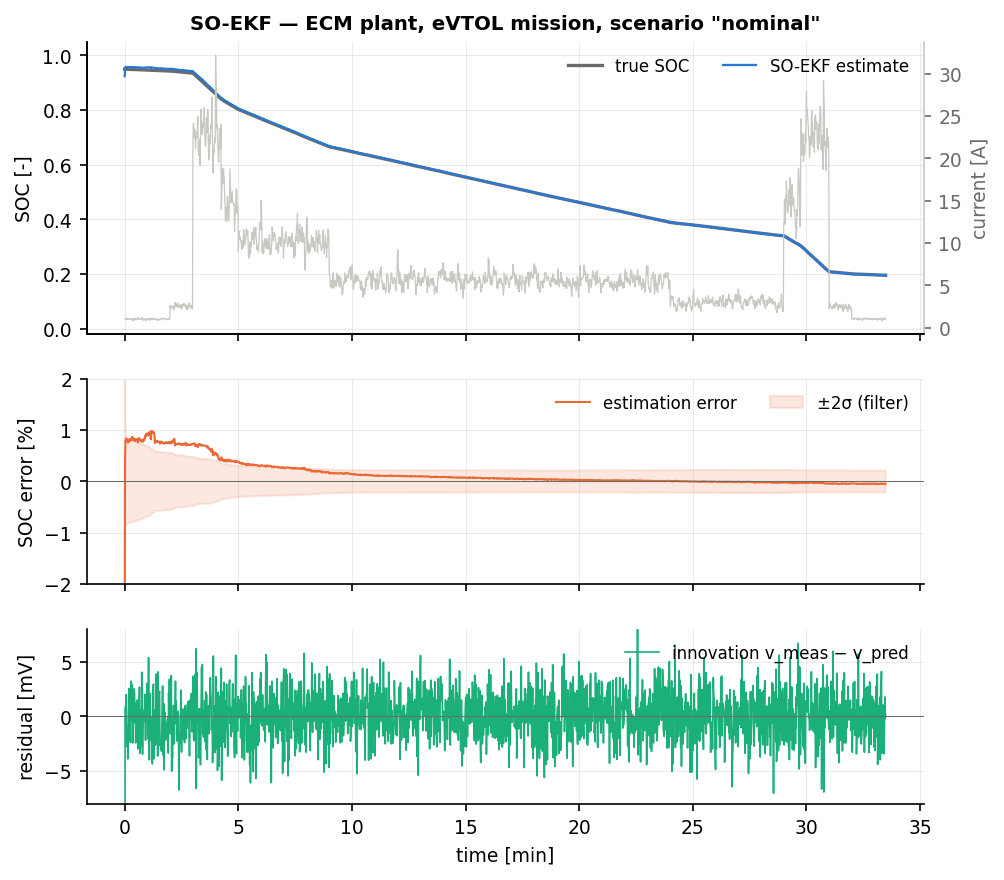
\includegraphics[width=\textwidth]{figures/cell_SOEKF_nominal.png}
\caption{SO-EKF on the nominal eVTOL mission: true and estimated SOC (top), estimation error with the $\pm 2\sigma$ band when available (middle), voltage residual (bottom).}
\end{figure}
\begin{figure}[H]\centering
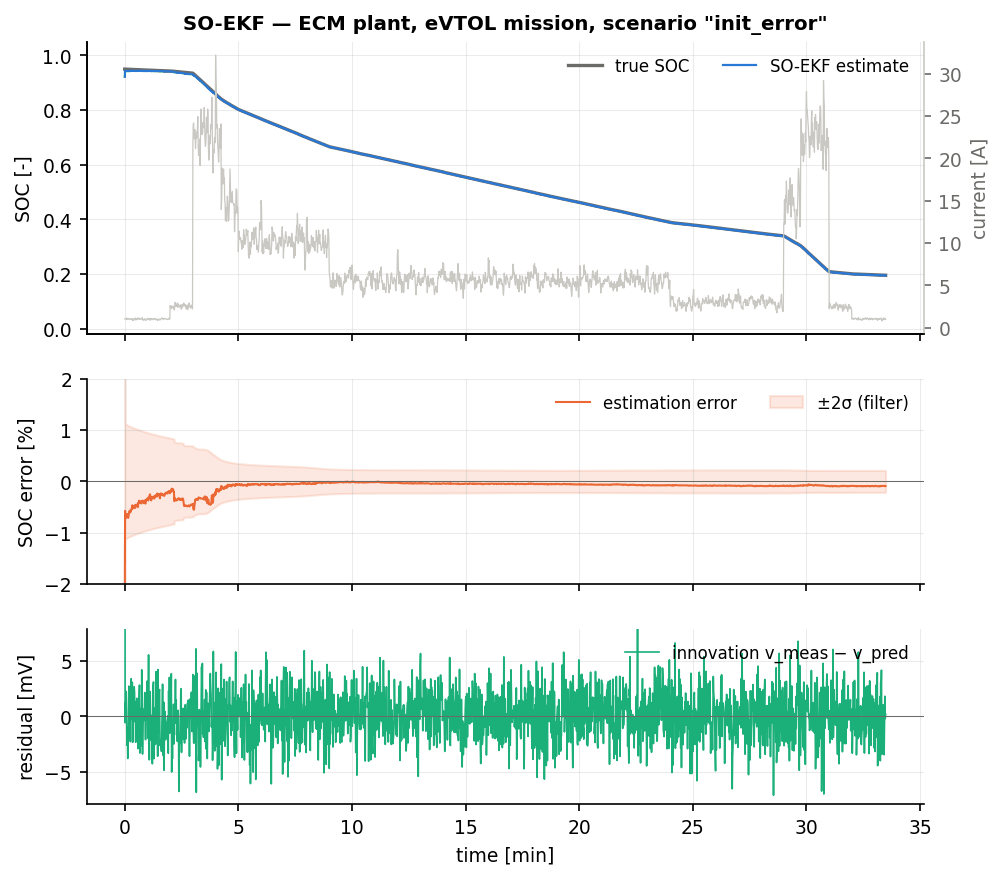
\includegraphics[width=\textwidth]{figures/cell_SOEKF_init_error.png}
\caption{SO-EKF with a 35\,\% initial SOC error.}
\end{figure}
\begin{figure}[H]\centering
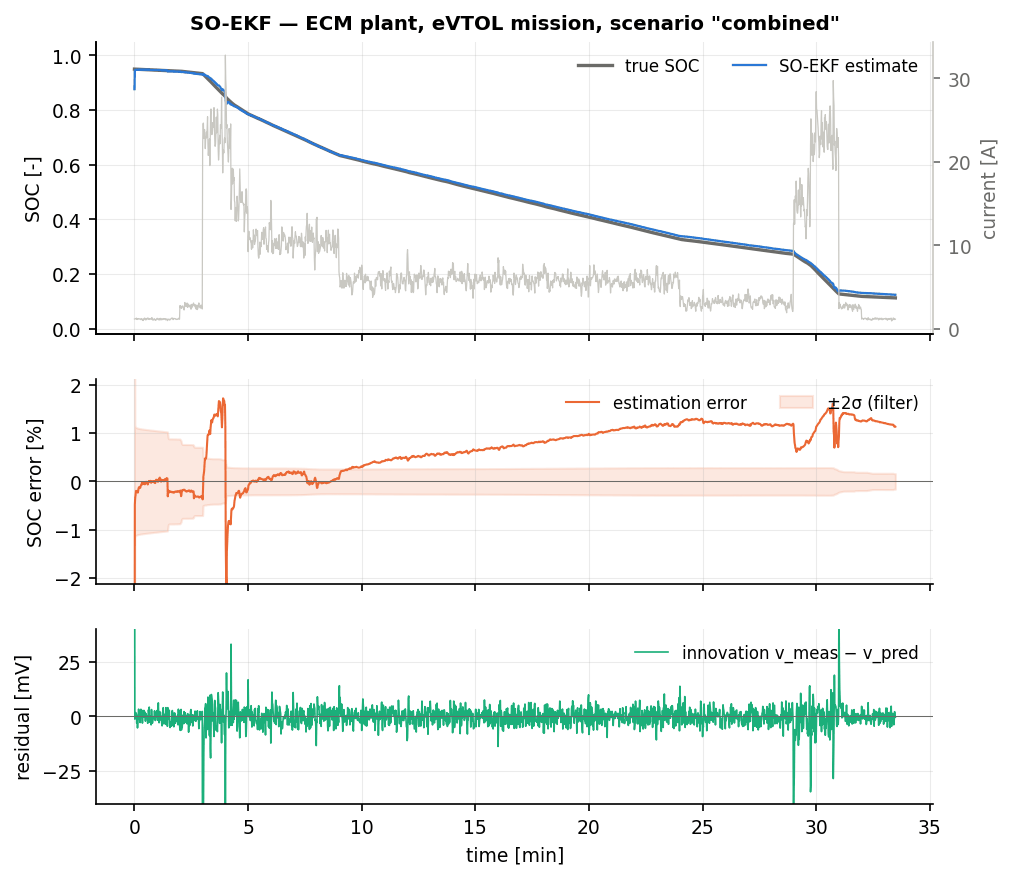
\includegraphics[width=\textwidth]{figures/cell_SOEKF_combined.png}
\caption{SO-EKF on the \texttt{combined} scenario: the explicit curvature term inflates $\tilde{\mR}$, the posterior variance does not collapse, and the filter finds the true SOC before the high-current segment.}
\end{figure}

All numbers are three-seed means in per cent SOC.

The SO-EKF is one of the three effective repairs of the EKF in this family. On
\texttt{combined} --- the scenario the EKF, CKF, CKF5, CDKF, GHKF, EIF, SR-EKF and UD-EKF all
fail --- it reaches $\text{RMSE} = 1.00\,\%$, $\text{RMSE}_{\text{ss}} = 1.28\,\%$ and
converges in the first sample, against the EKF's $16.02/12.44\,\%$ and never. It is
essentially tied with the UKF ($1.19\,\%$) and ahead of the IPLF ($1.72\,\%$) and the IEKF
($2.13\,\%$); the earlier development run, on a single seed, made the SO-EKF look twice as good
as the UKF, and the three-seed means show that the two are within their scatter of each other.
The mechanism is exactly \eqref{eq:soekf-battery}: at $k = 0$ the inflated $\tilde{R}$ prevents
the posterior variance from collapsing, the filter stays open to correction for the next few
seconds, and it finds the true SOC before the high-current segment begins.

It also gives the equal-best steady-state nominal accuracy of the family
($\text{RMSE}_{\text{ss}} = 0.04\,\%$, tied with the UKF and SR-UKF), the best
\texttt{sensor\_dropout} result of the fifteen ($0.36/0.18\,\%$ against the EKF's
$0.72/0.46\,\%$ --- the same inflation prevents the stuck voltage from being trusted), and a
large improvement on \texttt{param\_mismatch} ($0.77/0.89\,\%$ against $1.28/1.36\,\%$, second
only to the IPLF).

The cost appears in the whole-run metrics on easy scenarios: \texttt{nominal} RMSE $0.26\,\%$
against the EKF's $0.15\,\%$ and a maximum error of $3.95\,\%$ against $1.07\,\%$. All of this
is the deliberate caution of the first few seconds, when the second-order terms are large and
the filter correctly refuses to trust a measurement equation it knows is a poor affine model.
\texttt{outliers} degrades to $0.30\,\%$ steady state (EKF $0.21\,\%$) and \texttt{aged\_cell}
to $1.56\,\%$ (EKF $1.52\,\%$), the latter for the same reason as the IPLF: with a persistently
biased model, a filter that keeps its gain alive longer tracks the bias further.
\texttt{preisach} deserves a note: its steady-state error, $0.20\,\%$, is exactly the EKF's,
but its whole-run RMSE of $1.52\,\%$ is the worst of the family and its convergence time
($226$\,s) the longest, because the inflated $\tilde{\mR}$ makes it slow to take up the
hysteresis offset at the start of the mission.

The honest caveat is the step-size sensitivity documented above: within the physically
justified window $10^{-3}\le\rho\le10^{-2}$ the \texttt{combined} result varies by a factor of
two, so the headline $1.28\,\%$ should be read as ``order $1\,\%$, an order of magnitude better
than the EKF'', not as a precise figure. A model that supplied analytic Hessians --- trivial
here, since $\ocv''$ is available in closed form from the Chen2020 fit --- would remove the
sensitivity entirely, and that is the recommended production route. The divided-difference
filter of Chapter~\ref{ch:cdkf} offers the alternative: its second difference is taken over
$\pm\sqrt3\sigma$, i.e. a stencil that scales itself with the covariance and never needs a
step-size choice at all. The float-versus-double table shows the other side of the same coin:
the SO-EKF's nominal steady-state error rises from $0.03\,\%$ in double to $0.07\,\%$ in
single precision, the largest relative degradation of the EKF-family filters, because the
differencing amplifies round-off by $1/(4h_ah_b)\approx600$.

\paragraph{SPM plant: structured model error.}
\begin{figure}[H]\centering
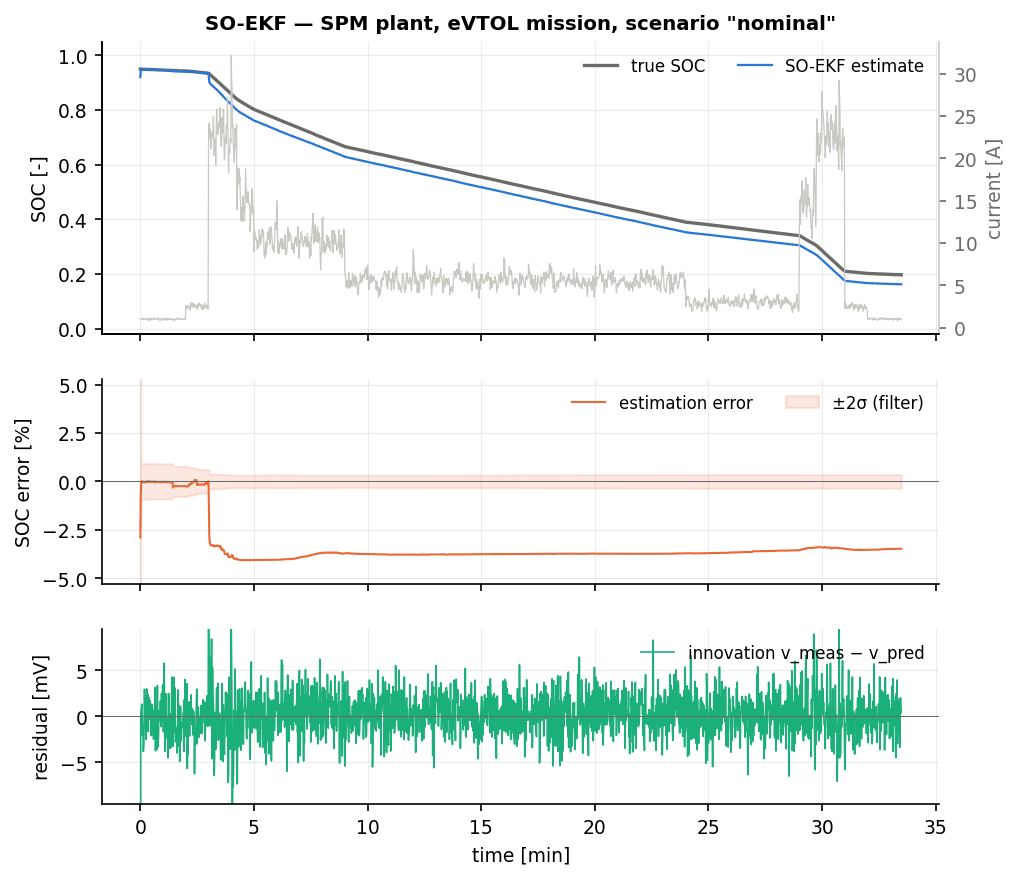
\includegraphics[width=\textwidth]{figures/cellspm_SOEKF_nominal.png}
\caption{SO-EKF on the nominal mission with the electrochemical (SPM) plant.}
\end{figure}
The SPM block of the table is a different kind of test. The plant is the electrochemical
single-particle model; the estimator still runs a 2-RC equivalent circuit, fitted to that plant,
which leaves a \emph{structured} residual of about $4$\,mV (Butler--Volmer kinetics and
solid-phase diffusion that no 2-RC circuit can reproduce) and a slow second branch,
$\tau_2 = 556$\,s. Over a $33$-minute mission a $556$\,s pole barely relaxes, so $v_2(t)$ is
close to an affine ramp --- and so is $\ocv(\soc(t))$ while the cell discharges at a roughly
constant rate. The two channels through which the measurement sees the state,
$(\partial\ocv/\partial\soc)\,\delta\soc$ and $-\delta v_2$, are therefore nearly collinear in
the information accumulated over the flight: the pair $(\soc, v_2)$ is close to unobservable,
and no filter can decide whether a persistent few-millivolt residual belongs to the slow RC
branch or to the state of charge. Because that direction is weakly observable, a $4$\,mV
structured error maps onto \emph{several per cent} of SOC instead of the
$4\,\text{mV}/0.8\,\text{V}\approx0.5\,\%$ a well-conditioned channel would give. This
$(\soc,v_2)$ ambiguity, not the size of the residual, is the mechanism behind the
$3.7$--$4.6\,\%$ band in which the whole classical family sits.

The SO-EKF is the best of the Jacobian-based filters on the SPM plant apart from the LKF:
$3.52\,\%$ on \texttt{nominal} against the EKF's $3.73\,\%$, $1.27\,\%$ on \texttt{outliers}
against $1.99\,\%$ (the best SPM outlier result of the family), $5.13\,\%$ on
\texttt{sensor\_dropout} against $5.31\,\%$ and $5.58\,\%$ on \texttt{current\_bias} against
$5.69\,\%$. The reason is the same inflation that wins \texttt{combined}: adding
$\tfrac12\tr(\nabla^2h\,\mP\,\nabla^2h\,\mP)$ to $\mR$ de-weights the OCV channel exactly when
$\sigma_\soc$ is large, which is precisely when the $(\soc,v_2)$ ambiguity is dangerous. The
effect is modest --- it does not lift the filter out of the band --- and it reverses on the two
rows where the prior stays wide for a long time: \texttt{cold} $8.16\,\%$ against the EKF's
$7.35\,\%$ and \texttt{param\_mismatch} $4.14\,\%$ against $3.13\,\%$. A curvature correction
addresses nonlinearity; the SPM residual is not curvature, it is a missing state.

\section{Summary}
The Gaussian second-order EKF adds two terms to the EKF: a bias correction
$\tfrac12\tr(\nabla^2h\,\mP)$ on the predicted measurement and an inflation
$\tfrac12\tr(\nabla^2h\,\mP\,\nabla^2h\,\mP)$ of the innovation covariance. On this benchmark
those two terms turn the EKF's worst failure into a result on a par with the UKF's, deliver the
equal-best steady-state nominal accuracy and the best \texttt{sensor\_dropout} result of all
fifteen filters, and cost about nine times an EKF step when the Hessians are computed
numerically (much less with analytic ones). Use it when the measurement function has
significant curvature over the prior --- which for an OCV-based SOC estimator is the case at
every cold start. Do not use a fixed finite-difference step on a look-up-table model without
checking the stencil against the table spacing, expect a visible penalty in single precision,
and remember that the second-order term helps with nonlinearity, not with model error: on the
SPM plant it gains $6\,\%$ relative to the EKF, not a factor.

% Copyright 2026 Sreeram Anil
% SPDX-License-Identifier: CC-BY-4.0
% =============================================================================
%  Cubature Kalman filter (third degree) — classical Kalman family
% =============================================================================
\chapter{Cubature Kalman Filter (CKF)}
\label{ch:ckf}

\section*{At a glance}
\begin{tabular}{@{}l>{\raggedright\arraybackslash}p{0.76\textwidth}@{}}
Family & classical Kalman (sigma-point) \\
Header & \texttt{include/estkit/filters/ckf.hpp} \\
Registered name & \texttt{CKF} \\
State dimension & $n_x = 4$ (cell model) --- generic in $n_x, n_u, n_y$ \\
Cubature points & $2n_x = 8$, equal weights $1/2n_x$, no tuning parameters \\
Cost per step & $\mathcal{O}(n_x^3)$ plus $4n_x$ model calls; $1.18$--$1.26\,\SI{}{\micro\second}$/step \\
Primary references & \cite{arasaratnam2009ckf,ito2000gaussian,sarkka2013} \\
\end{tabular}

\section{Motivation and aerospace/BMS relevance}
The unscented transform has three free parameters ($\alpha,\beta,\kappa$) whose ``correct''
values are the subject of a large and not always consistent literature, and for $n_x>3$ the
canonical choice $\kappa = 3-n_x$ makes the centre weight negative, so the transformed
covariance can lose positive definiteness. Arasaratnam and Haykin~\cite{arasaratnam2009ckf}
removed both problems by asking a different question: instead of designing a point set to
match moments, derive the numerically optimal cubature rule for the specific integral that a
Gaussian filter has to evaluate. The answer --- the third-degree spherical-radial rule --- is
parameter-free, has $2n_x$ points of \emph{equal positive} weight $1/(2n_x)$, and therefore
always produces a positive semi-definite covariance.

That combination (no tuning, guaranteed definiteness, derivative-free) is attractive for
certified software: there is no parameter for a reviewer to question and no failure branch to
justify. The CKF has become the default sigma-point filter in a large part of the aerospace
navigation literature for exactly this reason, and it is the natural baseline for the
square-root (Chapter~\ref{ch:sckf}) and fifth-degree (Chapter~\ref{ch:ckf5}) variants.

\section{Problem statement and assumptions}
Model \eqref{eq:ekf-proc}--\eqref{eq:ekf-meas} with additive noise. The Gaussian
(assumed-density) filter requires, at every step, integrals of the form
\begin{equation}
I[g] = \int_{\real^{n_x}} g(\vx)\, \N{\vx;\xhat}{\mP}\, d\vx,
\label{eq:ckf-integral}
\end{equation}
with $g$ ranging over $f$, $h$ and the outer products $ff^\T$, $hh^\T$ and $\vx h^\T$. No
differentiability of $g$ is needed --- only that the integrals exist. As for the UKF, the
filtering density is assumed to be adequately described by its first two moments.

\section{Derivation}
\paragraph{Spherical-radial decomposition.} Substituting $\vx = \xhat + \mS\vz$ with
$\mS\mS^\T = \mP$ turns \eqref{eq:ckf-integral} into a standard-Gaussian integral, and then
$\vz = r\bm{u}$ with $\norm{\bm{u}}=1$, $r\ge0$, splits it into a radial and a spherical
part:
\begin{equation}
I[g] = \frac{1}{(2\pi)^{n_x/2}}\int_0^\infty\!\!\int_{U_{n_x}} g(\xhat + \mS r\bm{u})\,
 r^{n_x-1}e^{-r^2/2}\,d\sigma(\bm{u})\,dr,
\label{eq:ckf-sr}
\end{equation}
where $U_{n_x}=\{\bm{u}: \bm{u}^\T\bm{u}=1\}$ and $\sigma$ is the spherical surface measure.
Arasaratnam and Haykin treat the two factors separately: the spherical integral by the
third-degree rule of Stroud~\cite{stroud1971}, which uses the $2n_x$ intersections of the
unit sphere with the coordinate axes and equal weights, and the radial integral --- after the
substitution $t = r^2/2$ a Gamma-weighted integral --- by the first-order Gauss--Laguerre
rule, which places a single node at $t = n_x/2$, i.e. $r = \sqrt{n_x}$. Combining the two,
\begin{equation}
I[g] \approx \frac{1}{2n_x}\sum_{i=1}^{2n_x} g\!\left(\xhat + \mS\,\bm{\xi}_i\right),
\qquad
\bm{\xi}_i = \sqrt{n_x}\,[\bm{1}]_i,
\label{eq:ckf-rule}
\end{equation}
where $[\bm{1}]_i$ runs over the $2n_x$ columns of $[\,\mI_{n_x}\; -\mI_{n_x}\,]$. The rule is
\emph{exact} for every monomial in $\vz$ of total degree $\le 3$: the zeroth moment gives
$\sum w_i = 1$, the second gives $\frac{1}{2n_x}\cdot 2\cdot n_x = 1$ per coordinate, and all
odd moments vanish by the central symmetry of the point set. It is not exact at degree four
($\sum w_i \xi_{i1}^4 = n_x$ versus the true value $3$), which is the source of the
differences with the fifth-degree rules discussed in Chapter~\ref{ch:ckf5}.

\begin{remark}[Relation to the UKF]
Setting $\alpha = 1$, $\kappa = 0$ in \eqref{eq:ukf-lambda} gives $\lambda = 0$,
$W_0^m = 0$, $W_{i} = 1/(2n_x)$ and points at $\pm\sqrt{n_x}$ standard deviations: the CKF is
exactly the scaled unscented transform with $\lambda = 0$ plus the deletion of the (zero
mean-weight) centre point. We used this identity as a cross-check: with $\alpha=1,\kappa=0$
the library UKF reproduces the CKF's benchmark behaviour on every scenario, which validates
both implementations.
\end{remark}

\paragraph{Filter recursion.} With $\mS^+ = \operatorname{chol}(\Pplus_{k-1})$,
\begin{align}
\mathcal{X}_i &= \xplus_{k-1} + \sqrt{n_x}\,\mS^+[\bm{1}]_i, &
\mathcal{X}^*_i &= f(\mathcal{X}_i,\vu_{k-1}), \label{eq:ckf-tu1}\\
\xminus_k &= \frac{1}{2n_x}\sum_i \mathcal{X}^*_i, &
\Pminus_k &= \frac{1}{2n_x}\sum_i(\mathcal{X}^*_i-\xminus_k)(\mathcal{X}^*_i-\xminus_k)^\T + \mQ,
\label{eq:ckf-tu2}
\end{align}
and, after regenerating the points from $(\xminus_k,\Pminus_k)$,
\begin{align}
\mathcal{Z}_i &= h(\mathcal{X}_i,\vu_k), \qquad \yhat_k = \frac{1}{2n_x}\sum_i \mathcal{Z}_i,
\label{eq:ckf-mu1}\\
\mP_{zz} &= \frac{1}{2n_x}\sum_i(\mathcal{Z}_i-\yhat_k)(\mathcal{Z}_i-\yhat_k)^\T + \mR,
\qquad
\mP_{xz} = \frac{1}{2n_x}\sum_i(\mathcal{X}_i-\xminus_k)(\mathcal{Z}_i-\yhat_k)^\T,
\label{eq:ckf-mu2}\\
\mW_k &= \mP_{xz}\mP_{zz}\inv, \quad
\xplus_k = \xminus_k + \mW_k(\vy_k-\yhat_k), \quad
\Pplus_k = \Pminus_k - \mW_k\mP_{zz}\mW_k^\T.
\label{eq:ckf-mu3}
\end{align}
The original paper writes the covariances as raw second moments minus the outer product of
the means; the implementation accumulates the centred deviations directly, which is
algebraically identical and avoids the cancellation $\overline{XX^\T}-\xhat\xhat^\T$ when the
mean is much larger than the spread --- relevant here, where $\soc\approx 1$ and
$\sigma_\soc\approx 10^{-3}$.

\section{Algorithm}
\begin{algorithm}[H]
\caption{CKF --- one sampling period (additive noise)}
\begin{algorithmic}[1]
\Require $\xplus_{k-1},\Pplus_{k-1},\vu_{k-1},\vy_k,\vu_k$
\State $\mS\gets\operatorname{chol}(\Pplus_{k-1})$;\;
       $\mathcal{X}_{i},\mathcal{X}_{i+n_x}\gets\xplus_{k-1}\pm\sqrt{n_x}\,\mS_{:,i}$, $i=1..n_x$
\State \textbf{Time update:} $\mathcal{X}_i\gets f(\mathcal{X}_i,\vu_{k-1})$;\;
       $\xminus_k\gets\frac{1}{2n_x}\sum_i\mathcal{X}_i$
\State $\Pminus_k\gets\frac{1}{2n_x}\sum_i(\mathcal{X}_i-\xminus_k)(\cdot)^\T+\mQ$; symmetrise
\State \textbf{Regenerate} $\mathcal{X}_i$ from $(\xminus_k,\Pminus_k)$;\;
       $\mathcal{Z}_i\gets h(\mathcal{X}_i,\vu_k)$;\; $\yhat_k\gets\frac{1}{2n_x}\sum_i\mathcal{Z}_i$
\State $\mP_{zz}\gets\frac{1}{2n_x}\sum_i(\mathcal{Z}_i-\yhat_k)(\cdot)^\T+\mR$;\;
       $\mP_{xz}\gets\frac{1}{2n_x}\sum_i(\mathcal{X}_i-\xminus_k)(\mathcal{Z}_i-\yhat_k)^\T$
\State $\mW\gets\mP_{xz}\mP_{zz}\inv$;\; $\xplus_k\gets\xminus_k+\mW(\vy_k-\yhat_k)$;\;
       $\Pplus_k\gets\Pminus_k-\mW\mP_{zz}\mW^\T$
\State \textbf{if} constraints enabled \textbf{then} $\xplus_k\gets\Pi(\xplus_k)$
\Ensure $\xplus_k,\Pplus_k$
\end{algorithmic}
\end{algorithm}

\section{Application to the battery model}
For $n_x=4$ the rule uses eight points at $\pm 2\sigma$ along the principal axes of $\mP$.
With the benchmark's initial covariance ($\sigma_\soc = 0.1$) the SOC points therefore sit at
$\soc_0 \pm 0.2$ --- a $40\,\%$ SOC span over which the NMC/graphite OCV curve is distinctly
non-affine. This is the single most important fact about the CKF on this problem: the
effective (statistical) measurement slope $\mP_{xz}/\mP_{\soc\soc}$ is then the \emph{chord}
of the OCV curve over $[\soc_0-0.2,\soc_0+0.2]$, not the tangent at $\soc_0$.

Options: none. \code{apply\_constraints = true} and \code{q\_scale = r\_scale = 1} are the
only knobs, and they exist for uniformity with the rest of the library, not because the
algorithm needs them.

\section{Implementation notes}
The eight points are stored in a \code{mutable} member array so that
\code{predict\_measurement} --- which the benchmark calls between \code{predict} and
\code{update} --- can regenerate them without copying the filter. The gain uses a direct
$n_y\times n_y$ inverse; for $n_y=1$ that is a division. Guard: if $\mW$ is not finite the
update is skipped and the prior is kept, so a degenerate $\mP_{zz}$ cannot inject NaN into
the state. Memory is 4560\,bytes; the per-step cost, $1.18$--$1.26\,\SI{}{\micro\second}$,
is $\approx 13\,\%$ below the UKF's $1.34$--$1.46$ because there are eight points instead of
nine and no weight arrays. In the single-precision build the results are identical to four decimals and
no covariance lost definiteness --- as guaranteed by the positive weights.

\section{Benchmark results}
\input{tables/cell_CKF.tex}
\begin{figure}[H]\centering
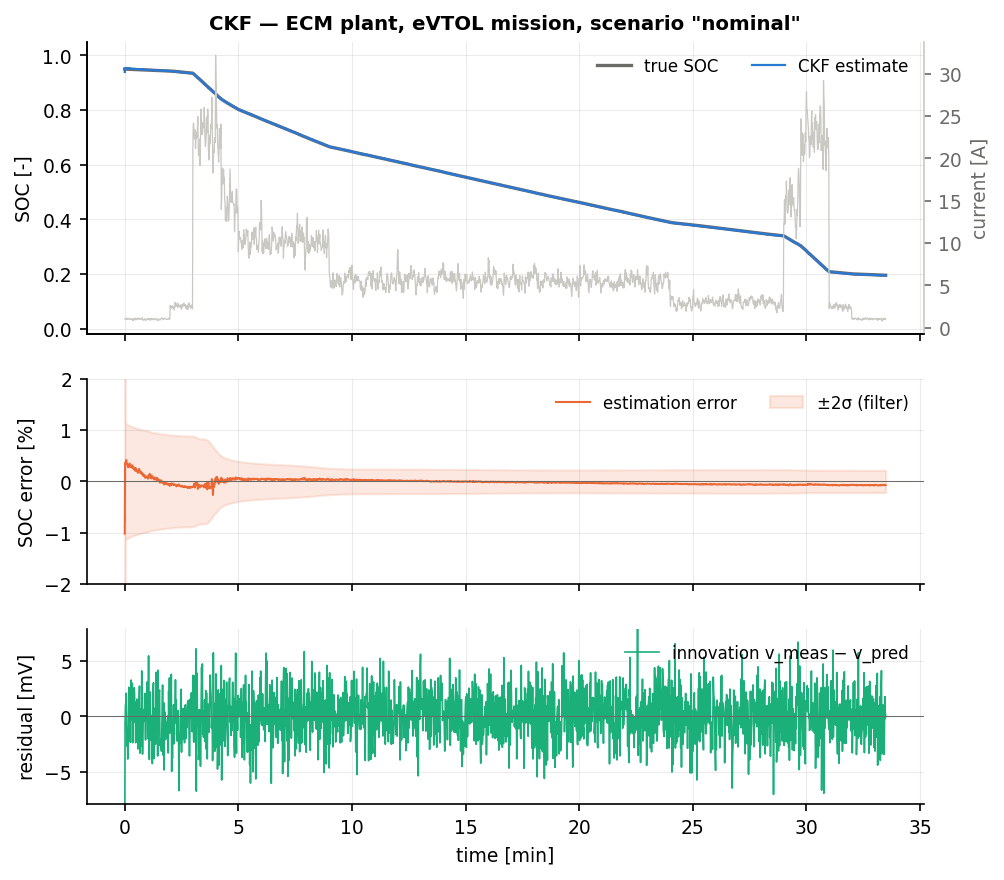
\includegraphics[width=\textwidth]{figures/cell_CKF_nominal.png}
\caption{CKF on the nominal eVTOL mission: true and estimated SOC (top), estimation error with the $\pm 2\sigma$ band when available (middle), voltage residual (bottom).}
\end{figure}
\begin{figure}[H]\centering
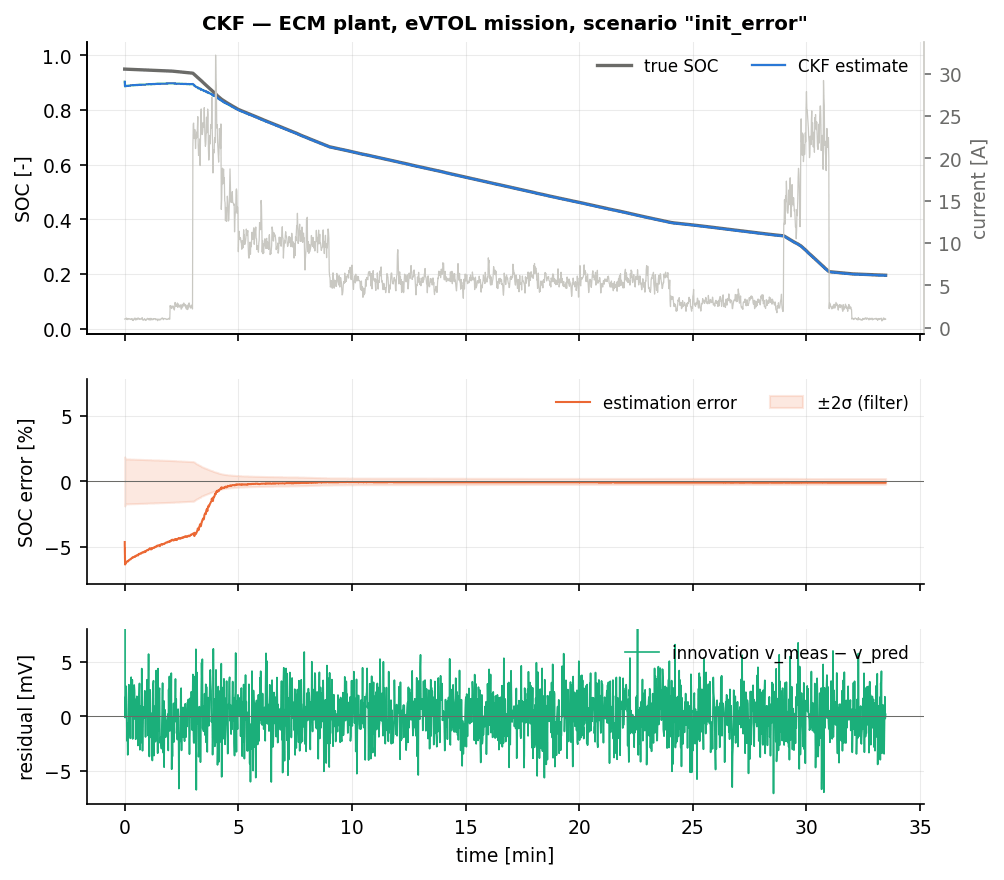
\includegraphics[width=\textwidth]{figures/cell_CKF_init_error.png}
\caption{CKF with a 35\,\% initial SOC error: the $\pm2\sigma$ point spread makes the statistical linearisation use the chord rather than the tangent of the OCV curve, and about $6\,\%$ of the initial error survives the first update.}
\end{figure}

All numbers are three-seed means in per cent SOC.

On \texttt{nominal} the CKF is the most accurate filter in the whole family over the full run:
$\text{RMSE} = 0.08\,\%$ against the EKF's $0.15\,\%$ and the UKF's $0.20\,\%$, with
$\text{RMSE}_{\text{ss}} = 0.05\,\%$ and a maximum error of $1.23\,\%$. It also has the best
\texttt{outliers} figure of the non-robust filters ($0.35/0.07\,\%$ against the EKF's
$0.52/0.21\,\%$), and it wins \texttt{current\_bias} ($0.55\,\%$ against $0.61\,\%$),
\texttt{cold} ($0.11\,\%$ against $0.16\,\%$) and \texttt{hot} is a wash. With a tight prior
the $\pm2\sigma$ points span only a few milli-SOC, the rule is then extremely accurate, and the
equal positive weights give a very clean covariance.

The same $\pm2\sigma$ spread is a liability when the prior is wide. On \texttt{init\_error}
($-35\,\%$) the CKF needs $221$\,s to bring the error below $2\,\%$, against $0$\,s for the EKF
and the UKF, and its whole-run RMSE is $1.64\,\%$ against the EKF's $0.14\,\%$ (the
steady-state value, $0.09\,\%$, is unaffected). The mechanism is the chord effect: with
$\soc_0 = 0.60$ the points sit at $0.40$ and $0.80$, the chord slope over that interval is
$\approx 0.98$\,V while the local slope is $0.80$\,V, so the correction is under-scaled by
$20\,\%$ and about $6\,\%$ of SOC error survives the first update; the prior then collapses and
the residual is removed only slowly by the subsequent small-gain updates. We verified that this
is a property of the point spread and not of the implementation by running the library UKF with
$\alpha = 1,\kappa = 0$ --- the same $\pm\sqrt{n_x}\sigma$ spread --- which reproduces the
behaviour.

The same weakness appears wherever the prior is forced open. \texttt{sensor\_dropout} gives
$2.83/1.92\,\%$ against the EKF's $0.72/0.46\,\%$ and the IEKF's $0.37/0.19\,\%$ --- the worst
of the fifteen --- because during the $15$\,s of stuck voltage the covariance grows and the
wide point set then mis-scales the recovery. \texttt{aged\_cell} is $2.87/1.79\,\%$ against the
EKF's $1.18/1.52\,\%$ and the fifth-degree rules' $2.50/1.54\,\%$: the third-degree rule
over-estimates the fourth moment by $n_x/3$, which inflates $\mP_{zz}$ asymmetrically once the
model bias has widened the prior. Raising the rule to fifth degree
(Chapter~\ref{ch:ckf5}) recovers most of that. \texttt{param\_mismatch} is $1.59\,\%$ against
the EKF's $1.36\,\%$ and \texttt{preisach} $0.24\,\%$ against $0.20\,\%$, with a convergence
time of $218$\,s against $16$\,s --- the hysteresis offset is taken up slowly for the same
chord reason.

On \texttt{combined} the CKF fails as the EKF does ($\text{RMSE}_{\text{ss}} = 11.26\,\%$,
never converges, peak error $23.2\,\%$). It shares the EKF's mechanism --- the posterior
variance collapses after the first update and the estimate is then locked in against a $25\,\%$
unmodelled rise in $R_0$ --- and the cubature rule does nothing to prevent it because, unlike
the $\alpha = 0.1$ UKF, it does not over-inflate $\mP_{zz}$ (see Remark~\ref{rm:ukf-w0}).

\paragraph{SPM plant: structured model error.}
\begin{figure}[H]\centering
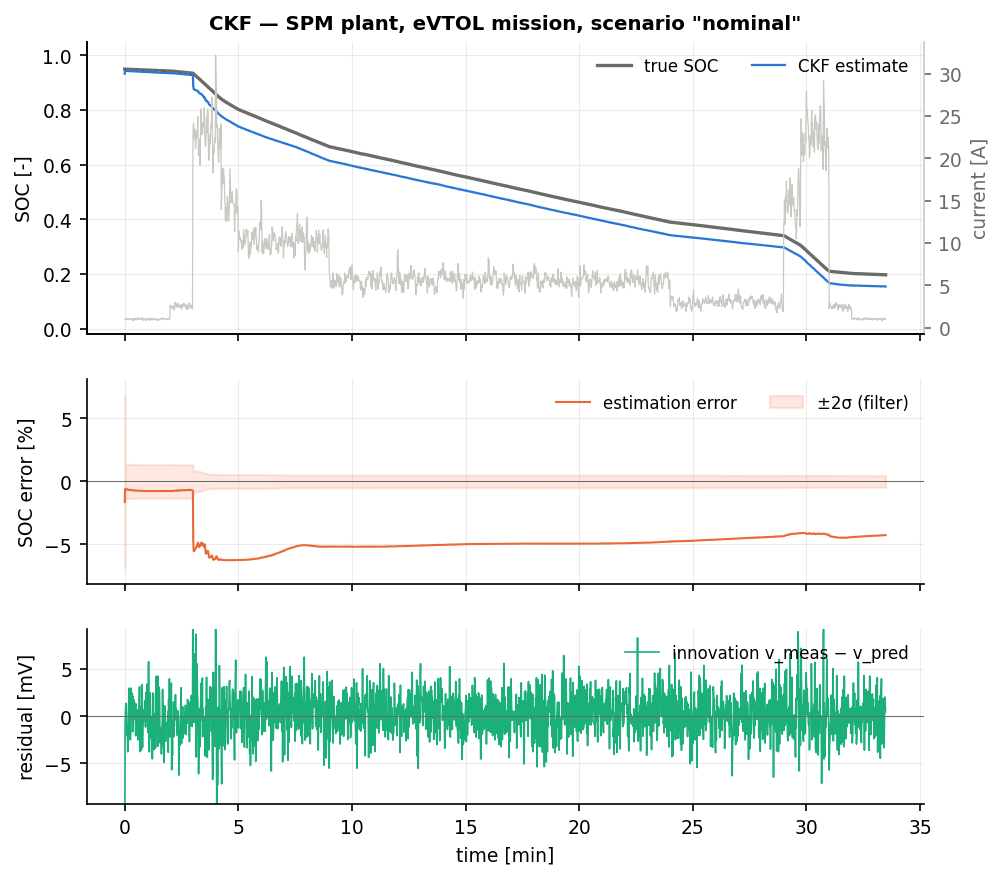
\includegraphics[width=\textwidth]{figures/cellspm_CKF_nominal.png}
\caption{CKF on the nominal mission with the electrochemical (SPM) plant.}
\end{figure}
The SPM block of the table is a different kind of test. The plant is the electrochemical
single-particle model; the estimator still runs a 2-RC equivalent circuit, fitted to that plant,
which leaves a \emph{structured} residual of about $4$\,mV (Butler--Volmer kinetics and
solid-phase diffusion that no 2-RC circuit can reproduce) and a slow second branch,
$\tau_2 = 556$\,s. Over a $33$-minute mission a $556$\,s pole barely relaxes, so $v_2(t)$ is
close to an affine ramp --- and so is $\ocv(\soc(t))$ while the cell discharges at a roughly
constant rate. The two channels through which the measurement sees the state,
$(\partial\ocv/\partial\soc)\,\delta\soc$ and $-\delta v_2$, are therefore nearly collinear in
the information accumulated over the flight: the pair $(\soc, v_2)$ is close to unobservable,
and no filter can decide whether a persistent few-millivolt residual belongs to the slow RC
branch or to the state of charge. Because that direction is weakly observable, a $4$\,mV
structured error maps onto \emph{several per cent} of SOC instead of the
$4\,\text{mV}/0.8\,\text{V}\approx0.5\,\%$ a well-conditioned channel would give. This
$(\soc,v_2)$ ambiguity, not the size of the residual, is the mechanism behind the
$3.7$--$4.6\,\%$ band in which the whole classical family sits.

The cubature filters are the \emph{worst} of the family here: $4.62\,\%$ on SPM
\texttt{nominal} against the EKF's $3.73\,\%$ and the LKF's $1.72\,\%$, $8.72\,\%$ on
\texttt{cold} against $7.35\,\%$, $8.24\,\%$ on \texttt{sensor\_dropout} against $5.31\,\%$ and
$4.81\,\%$ on \texttt{param\_mismatch} against $3.13\,\%$. The ordering across the whole family
is in fact monotone in the sigma-point spread --- LKF (frozen tangent) $1.72$, EKF/IEKF
(tangent at the mean) $3.66$--$3.73$, UKF ($0.2\sigma$ points) $3.96$, cubature filters
($2\sigma$ or $2.45\sigma$ points) $4.61$--$4.62$ --- and the ambiguity argument explains it.
A statistical linearisation taken over a wide prior returns the \emph{chord} of the OCV curve,
which is steeper than the tangent over most of the mission, so the filter believes the OCV
channel is more informative than it is and commits harder to the direction that carries the
structured error. The single exception is \texttt{outliers} ($2.21\,\%$), where every filter
does better on SPM than on ECM because the corrupted samples widen the effective innovation
covariance. Nothing diverges and $t_{\text{conv}} = 0$ on every SPM row: the error is a bias,
not a drift.

\section{Summary}
The CKF is the sigma-point filter to reach for when you want no tuning parameters and a
provably positive semi-definite covariance: it is cheaper than the UKF
($1.18$--$1.26\,\SI{}{\micro\second}$ against $1.34$--$1.46$), derivative-free, and on this
benchmark the most accurate filter of all under nominal ECM conditions. Its weakness is the
fixed $\pm\sqrt{n_x}\sigma$ point spread, which makes the statistical linearisation use the
chord rather than the tangent of a curved measurement function; with a wide prior (large
initial SOC error, sensor dropout, strong model mismatch) it converges noticeably more slowly
than an EKF, is the worst of the family on \texttt{sensor\_dropout}, and is the worst of the
family on the SPM plant. Use the square-root form (Chapter~\ref{ch:sckf}) in single precision
and the fifth-degree form (Chapter~\ref{ch:ckf5}) when the prior is wide.

% Copyright 2026 Sreeram Anil
% SPDX-License-Identifier: CC-BY-4.0
% =============================================================================
%  Fifth-degree cubature Kalman filter — classical Kalman family
% =============================================================================
\chapter{Fifth-Degree Cubature Kalman Filter (CKF5)}
\label{ch:ckf5}

\section*{At a glance}
\begin{tabular}{@{}l>{\raggedright\arraybackslash}p{0.76\textwidth}@{}}
Family & classical Kalman (sigma-point) \\
Header & \texttt{include/estkit/filters/ckf\_high\_degree.hpp} \\
Registered name & \texttt{CKF5} \\
State dimension & $n_x = 4$ (cell model) --- generic in $n_x, n_u, n_y$ \\
Cubature points & $2n_x^2+1 = 33$ \\
Cost per step & $\mathcal{O}(n_x^4)$ plus $2(2n_x^2{+}1)$ model calls; $3.7$--$4.1\,\SI{}{\micro\second}$/step \\
Primary references & \cite{jia2013highdegree,arasaratnam2009ckf,stroud1971} \\
\end{tabular}

\section{Motivation and aerospace/BMS relevance}
The third-degree cubature rule of Chapter~\ref{ch:ckf} integrates cubic polynomials exactly;
its leading error term is therefore proportional to the fourth derivative of the integrand
times the fourth moment of the prior, i.e. to $\partial^4 g/\partial x^4 \cdot \sigma^4$.
When $\sigma$ is small this is negligible --- and the benchmark confirms it, the CKF being the
most accurate filter under nominal conditions. When $\sigma$ is large, as it is after a
power-up with unknown SOC or when an unmodelled capacity loss widens the prior, the fourth
order term dominates and a higher-degree rule is the systematic cure.

Jia, Xin and Cheng~\cite{jia2013highdegree} give a constructive recipe for arbitrary odd
degree by combining a Gauss--Chebyshev radial rule with a degree-matched spherical rule. The
fifth-degree member costs $2n_x^2+1$ points instead of $2n_x$ --- $33$ instead of $8$ for the
cell model --- which is affordable at small $n_x$ and is the natural point to stop: the
seventh-degree rule needs $\mathcal{O}(n_x^3)$ points and acquires large negative weights.

\section{Problem statement and assumptions}
Model \eqref{eq:ekf-proc}--\eqref{eq:ekf-meas}, additive noise, Gaussian assumed density; the
integrals to evaluate are \eqref{eq:ckf-integral}. In addition, for the rule to be useful the
prior must be well approximated by a Gaussian over the span of the points, which now reach
$\sqrt{n_x+2} = 2.45$ standard deviations along the axes.

\section{Derivation}
After the substitution $\vx = \xhat + \mS\vz$, everything reduces to the standard-normal
integral $\int g(\vz)\N{\vz;\bm{0}}{\mI}d\vz$. A \emph{fully symmetric} rule of degree five
for this weight uses three orbits: the origin, the $2n$ axial points $\pm\sqrt{c}\,\bm{e}_i$,
and the $2n(n-1)$ ``diagonal'' points $\sqrt{c}(\pm\bm{e}_k\pm\bm{e}_l)/\sqrt2$, $k<l$. Writing
$n = n_x$ and $c = n+2$, the rule is
\begin{align}
\int g(\vz)\,\N{\vz;\bm{0}}{\mI}\,d\vz \;\approx\;
& w_0\, g(\bm{0})
+ w_1 \sum_{i=1}^{n}\sum_{s=\pm1} g\!\left(s\sqrt{n{+}2}\,\bm{e}_i\right) \nonumber\\
&+ w_2 \sum_{k<l}\ \sum_{s,t=\pm1} g\!\left(\sqrt{\tfrac{n+2}{2}}\,(s\bm{e}_k + t\bm{e}_l)\right),
\label{eq:ckf5-rule}
\end{align}
\begin{equation}
w_0 = \frac{2}{n+2}, \qquad
w_1 = \frac{4-n}{2(n+2)^2}, \qquad
w_2 = \frac{1}{(n+2)^2},
\label{eq:ckf5-weights}
\end{equation}
with $1 + 2n + 2n(n-1) = 2n^2+1$ points in total. All odd moments vanish by the central
symmetry of the point set; the even moments are verified directly:
\begin{align}
\textstyle\sum w &= w_0 + 2n w_1 + 2n(n-1) w_2 = \frac{2}{n+2} + \frac{4-n}{n+2} + \frac{2(n-1)}{n+2} = 1,
\label{eq:ckf5-m0}\\
\textstyle\sum w\,z_1^2 &= 2(n{+}2)w_1 + 2(n{-}1)(n{+}2)w_2 = \frac{4-n}{n+2}+\frac{2(n-1)}{n+2} = 1,
\label{eq:ckf5-m2}\\
\textstyle\sum w\,z_1^4 &= 2(n{+}2)^2 w_1 + (n{-}1)(n{+}2)^2 w_2 = (4-n) + (n-1) = 3,
\label{eq:ckf5-m4}\\
\textstyle\sum w\,z_1^2z_2^2 &= 4\cdot\tfrac{(n+2)^2}{4}\,w_2 = 1,
\label{eq:ckf5-m22}
\end{align}
matching $\E{z_1^2}=1$, $\E{z_1^4}=3$, $\E{z_1^2z_2^2}=1$ of the standard normal, so
\eqref{eq:ckf5-rule} is exact for every monomial of total degree $\le5$. Contrast
\eqref{eq:ckf5-m4} with the third-degree rule, for which $\sum w z_1^4 = n$: for $n_x = 4$ the
CKF over-estimates the fourth moment by $33\,\%$ and the CKF5 gets it exactly right.

\begin{remark}[$n_x = 4$ is a special case]\label{rm:ckf5-n4}
$w_1 = (4-n)/(2(n+2)^2)$ vanishes identically at $n = 4$: the eight axial points carry zero
weight and the rule effectively uses the origin plus the $24$ diagonal points. For $n > 4$
the axial weight is \emph{negative}, so the sample covariance is no longer guaranteed
positive semi-definite --- the generic price of high-degree rules. The implementation keeps
the axial points (and evaluates them) for clarity and genericity; their contribution is
multiplied by zero at $n_x=4$.
\end{remark}

\paragraph{Filter recursion.} Identical in structure to \eqref{eq:ckf-tu1}--\eqref{eq:ckf-mu3}
with the equal weights $1/(2n_x)$ replaced by the $w_i$ of \eqref{eq:ckf5-weights} and the
points of \eqref{eq:ckf5-rule} mapped through $\mS$:
\begin{equation}
\mathcal{X}_i = \xhat + \mS\bm{\xi}_i, \qquad
\xminus = \sum_i w_i f(\mathcal{X}_i,\vu), \qquad
\Pminus = \sum_i w_i (f(\mathcal{X}_i,\vu)-\xminus)(\cdot)^\T + \mQ,
\label{eq:ckf5-recursion}
\end{equation}
and likewise for the measurement update.

\section{Algorithm}
\begin{algorithm}[H]
\caption{CKF5 --- one sampling period (additive noise)}
\begin{algorithmic}[1]
\Require $\xplus_{k-1},\Pplus_{k-1},\vu_{k-1},\vy_k,\vu_k$; weights \eqref{eq:ckf5-weights} precomputed
\State $\mS\gets\operatorname{chol}(\Pplus_{k-1})$;\;
       $\gamma_1\gets\sqrt{n_x+2}$,\; $\gamma_2\gets\gamma_1/\sqrt2$
\State $\mathcal{X}_0\gets\xplus_{k-1}$;\;
       $\mathcal{X}\gets\xplus_{k-1}\pm\gamma_1\mS_{:,i}$ ($2n_x$ points);\;
       $\mathcal{X}\gets\xplus_{k-1}\pm\gamma_2\mS_{:,k}\pm\gamma_2\mS_{:,l}$ ($2n_x(n_x{-}1)$ points)
\State \textbf{Time update:} $\mathcal{X}_i\gets f(\mathcal{X}_i,\vu_{k-1})$;\;
       $\xminus_k\gets\sum_i w_i\mathcal{X}_i$;\;
       $\Pminus_k\gets\sum_i w_i(\mathcal{X}_i-\xminus_k)(\cdot)^\T+\mQ$
\State \textbf{Regenerate} the point set from $(\xminus_k,\Pminus_k)$;\;
       $\mathcal{Z}_i\gets h(\mathcal{X}_i,\vu_k)$;\; $\yhat_k\gets\sum_i w_i\mathcal{Z}_i$
\State $\mP_{zz}\gets\sum_i w_i(\mathcal{Z}_i-\yhat_k)(\cdot)^\T+\mR$;\;
       $\mP_{xz}\gets\sum_i w_i(\mathcal{X}_i-\xminus_k)(\mathcal{Z}_i-\yhat_k)^\T$
\State $\mW\gets\mP_{xz}\mP_{zz}\inv$;\; $\xplus_k\gets\xminus_k+\mW(\vy_k-\yhat_k)$;\;
       $\Pplus_k\gets\Pminus_k-\mW\mP_{zz}\mW^\T$
\State \textbf{if} constraints enabled \textbf{then} $\xplus_k\gets\Pi(\xplus_k)$
\Ensure $\xplus_k,\Pplus_k$
\end{algorithmic}
\end{algorithm}

\section{Application to the battery model}
With $n_x = 4$ the filter uses $33$ points, of which $25$ carry weight
(Remark~\ref{rm:ckf5-n4}): the mean with $w_0 = 1/3$ and $24$ diagonal points with
$w_2 = 1/36$ each. The diagonal points mix pairs of states, so the SOC channel is probed at
$\soc \pm \sqrt{3}\,\sigma_\soc$ simultaneously with a perturbation in $v_1$, $v_2$ or $h$ ---
which is exactly what is needed to capture the cross-curvature of $h$, although for this
model $h$ is bilinear-free (the only curvature is $\partial^2\ocv/\partial\soc^2$).

The dominant cost is $66$ evaluations of the cell model per step, each containing three
exponentials and an OCV table look-up; that is the whole explanation of the measured
$3.7$--$4.1\,\SI{}{\micro\second}$ per step, roughly $3\times$ the third-degree CKF and
$8\times$ the EKF. The moment sums themselves cost $33$ rank-one updates of a $4\times4$
matrix, i.e. $\mathcal{O}(n_x^4)$, which starts to dominate for $n_x \gtrsim 12$.

\section{Implementation notes}
The weights are computed once in the constructor and stored in a $33$-entry array; the point
set is regenerated every call from the current Cholesky factor. Zero-weight points are
evaluated rather than skipped, which costs $24\,\%$ of the runtime at $n_x=4$ and keeps the
code branch-free and obviously correct; a production implementation for a fixed $n_x=4$ would
drop them. For $n_x>4$ the negative axial weight can make the sample covariance indefinite;
the implementation relies on (i) adding $\mQ$ (resp.\ $\mR$) after the sum and (ii)
\code{cholesky\_safe}'s jitter fall-back, and the chapter's recommendation is to prefer the
third-degree square-root filter beyond $n_x\approx8$. Memory is 5624\,bytes, the largest of
the non-quadrature filters, because the $33$ propagated points are stored as members.

\section{Benchmark results}
% Copyright 2026 Sreeram Anil
% SPDX-License-Identifier: CC-BY-4.0
\begin{table}[H]\centering\footnotesize\setlength{\tabcolsep}{4pt}
\caption{CKF5: cell-level benchmark on the eVTOL mission (mean over seeds; RMSE and max error in \% SOC; $t_\mathrm{conv}$: first time the error stays below 2\,\% for 60\,s, -- = never; EKF reference: steady-state RMSE of the plain EKF on the same data).}\label{tab:cell_CKF5}
\begin{tabular}{llrrrrrcrr}\toprule
plant & scenario & RMSE & RMSE$_\mathrm{ss}$ & max & $t_\mathrm{conv}$ [s] & RMSE$_v$ [mV] & div. & EKF ref. & ns/step \\ \midrule
ECM & nominal & 0.08 & 0.05 & 1.70 & 0 & 0.81 & no & 0.05 & 4014 \\
ECM & init\_error & 1.85 & 0.12 & 7.33 & 229 & 2.11 & no & 0.05 & 4027 \\
ECM & current\_bias & 0.48 & 0.55 & 1.47 & 0 & 0.87 & no & 0.61 & 4032 \\
ECM & noise\_step & 0.14 & 0.14 & 1.70 & 0 & 2.89 & no & 0.12 & 4015 \\
ECM & outliers & 0.31 & 0.08 & 4.66 & 0 & 2.10 & no & 0.21 & 4021 \\
ECM & cold & 0.16 & 0.09 & 1.58 & 0 & 1.90 & no & 0.16 & 4013 \\
ECM & hot & 0.08 & 0.04 & 1.73 & 0 & 0.57 & no & 0.03 & 4024 \\
ECM & aged\_cell & 2.50 & 1.54 & 8.47 & 0 & 3.80 & no & 1.52 & 4025 \\
ECM & param\_mismatch & 1.84 & 1.79 & 5.19 & 0 & 2.83 & no & 1.36 & 4019 \\
ECM & sensor\_dropout & 2.75 & 1.86 & 7.45 & 0 & 1.86 & no & 0.46 & 4019 \\
ECM & preisach & 1.27 & 0.24 & 4.36 & 217 & 0.86 & no & 0.20 & 4024 \\
ECM & combined & 14.64 & 11.96 & 24.59 & -- & 5.12 & no & 12.44 & 4087 \\
\midrule
SPM & nominal & 4.70 & 4.61 & 6.13 & 0 & 1.04 & no & 3.73 & 3795 \\
SPM & init\_error & 5.26 & 4.68 & 7.33 & -- & 2.17 & no & 3.81 & 3761 \\
SPM & current\_bias & 6.05 & 6.63 & 7.46 & 0 & 1.13 & no & 5.69 & 3779 \\
SPM & noise\_step & 4.25 & 3.76 & 6.13 & 0 & 3.15 & no & 3.30 & 3767 \\
SPM & outliers & 2.26 & 2.27 & 5.67 & -- & 2.33 & no & 1.99 & 3740 \\
SPM & cold & 8.66 & 8.74 & 10.80 & -- & 4.23 & no & 7.35 & 3700 \\
SPM & hot & 2.71 & 2.71 & 3.36 & 0 & 0.72 & no & 2.16 & 3749 \\
SPM & param\_mismatch & 4.66 & 4.90 & 5.73 & 0 & 1.98 & no & 3.13 & 3763 \\
SPM & sensor\_dropout & 8.11 & 8.24 & 9.74 & 0 & 1.93 & no & 5.31 & 3757 \\
\bottomrule\end{tabular}\end{table}

\begin{figure}[H]\centering
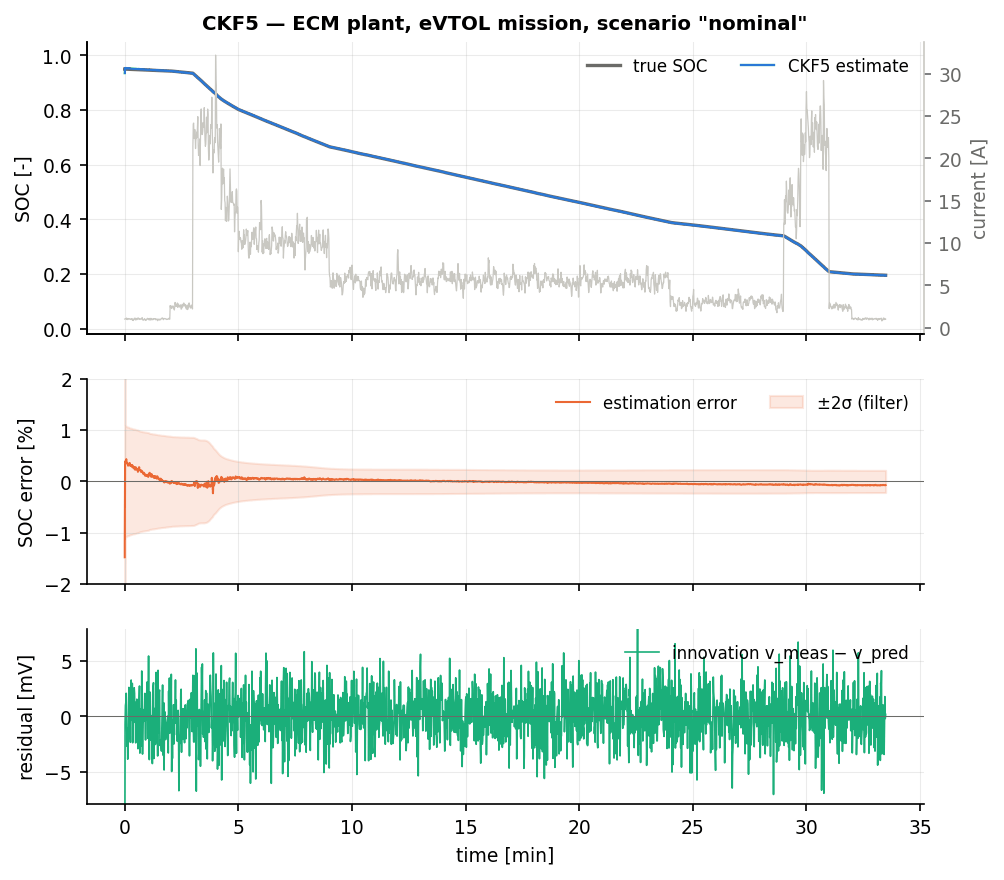
\includegraphics[width=\textwidth]{figures/cell_CKF5_nominal.png}
\caption{CKF5 on the nominal eVTOL mission: true and estimated SOC (top), estimation error with the $\pm 2\sigma$ band when available (middle), voltage residual (bottom).}
\end{figure}
\begin{figure}[H]\centering
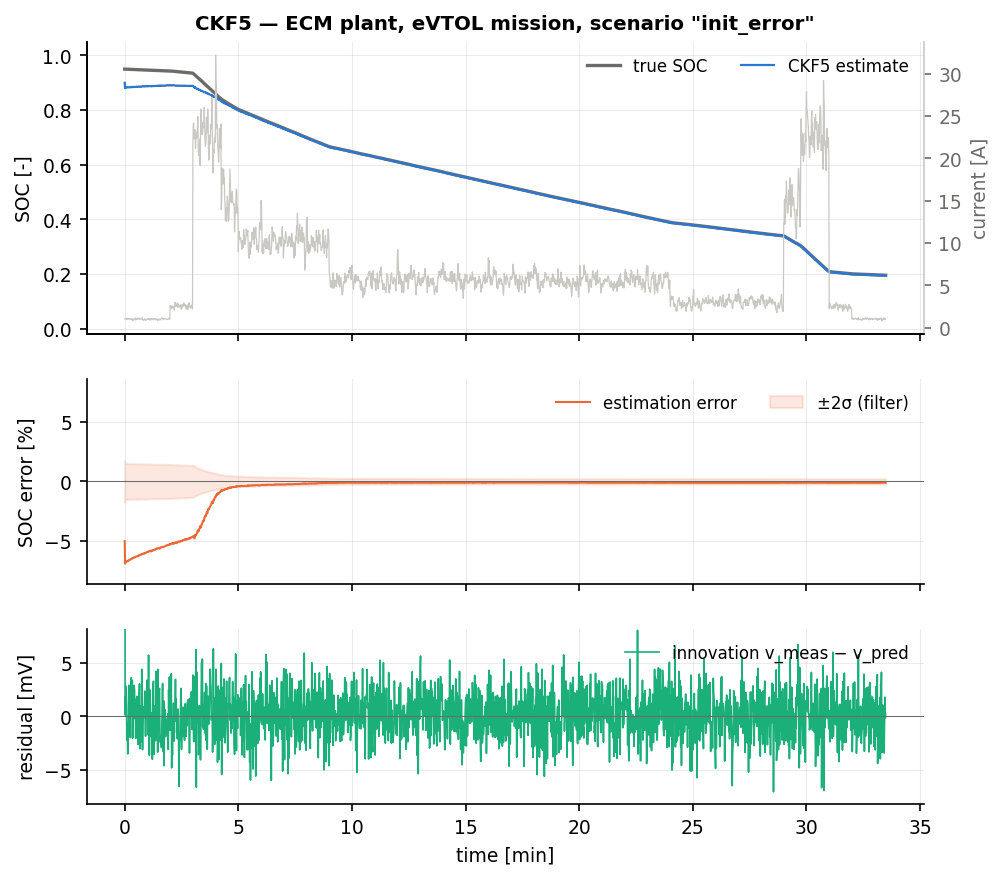
\includegraphics[width=\textwidth]{figures/cell_CKF5_init_error.png}
\caption{CKF5 with a 35\,\% initial SOC error.}
\end{figure}

All numbers are three-seed means in per cent SOC.

The most striking result is not in any single column but in the comparison across chapters:
\textbf{the CKF5, the DD2/CDKF (Chapter~\ref{ch:cdkf}) and the $3$-point Gauss--Hermite filter
(Chapter~\ref{ch:ghkf}) produce identical metrics to two decimals in all twelve ECM scenarios
and all nine SPM scenarios.} These are three independently derived rules --- a spherical-radial
cubature rule, a Stirling interpolation with step $h = \sqrt3$, and a tensor-product quadrature
--- that all integrate polynomials up to degree five exactly and all place their points at
$\sqrt3$ or $\sqrt{n_x+2}$ standard deviations. Their agreement is a strong mutual validation
of the three implementations and a concrete illustration of the ``numerical integration
perspective'' on Gaussian filters~\cite{wu2006numerical}: once the degree of exactness is
fixed, the specific rule matters far less than the degree.

Against the third-degree CKF the fifth-degree rule helps where the theory says it should ---
when the prior is wide. \texttt{aged\_cell}: $2.50/1.54\,\%$ against the CKF's $2.87/1.79\,\%$,
with the peak error falling from $9.6\,\%$ to $8.0\,\%$, which brings it level with the EKF
($1.18/1.52\,\%$). \texttt{outliers}: $0.31/0.08\,\%$, with $t_{\text{conv}} = 0$ against the
CKF's $4$\,s. Where the prior is tight the two are indistinguishable: \texttt{nominal}
$0.08/0.05\,\%$ for both, and \texttt{cold}, \texttt{hot}, \texttt{current\_bias},
\texttt{noise\_step} and \texttt{preisach} agree to within a hundredth of a per cent.

It is not uniformly better. \texttt{init\_error} is marginally worse ($1.85/0.12\,\%$,
$t_{\text{conv}} = 229$\,s, against $1.64/0.09\,\%$ and $221$\,s), because the higher-degree
rule reaches further ($\sqrt{n_x+2} = 2.45\sigma$ against $2\sigma$) into a region where the
OCV curve is not polynomial at all. \texttt{param\_mismatch} is worse ($1.84/1.79\,\%$ against
$1.56/1.59\,\%$) and \texttt{combined} is worse ($14.64/11.96\,\%$ against $13.07/11.26\,\%$);
both are model-error scenarios in which integrating the \emph{wrong} model more accurately is
no help --- a point worth keeping in mind whenever a higher-order filter is proposed as a cure
for a modelling problem. \texttt{sensor\_dropout} is a wash at $2.75/1.86\,\%$ against
$2.83/1.92\,\%$, both far behind the EKF's $0.72/0.46\,\%$.

\paragraph{SPM plant: structured model error.}
\begin{figure}[H]\centering
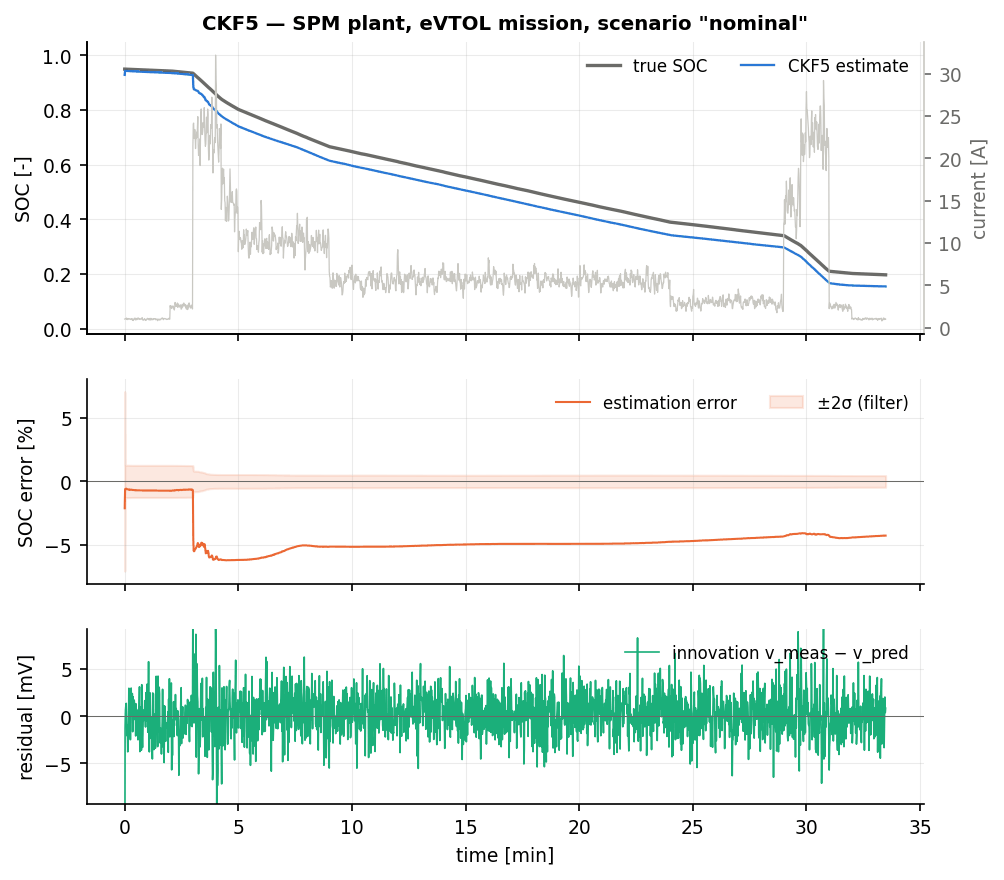
\includegraphics[width=\textwidth]{figures/cellspm_CKF5_nominal.png}
\caption{CKF5 on the nominal mission with the electrochemical (SPM) plant.}
\end{figure}
The SPM block of the table is a different kind of test. The plant is the electrochemical
single-particle model; the estimator still runs a 2-RC equivalent circuit, fitted to that plant,
which leaves a \emph{structured} residual of about $4$\,mV (Butler--Volmer kinetics and
solid-phase diffusion that no 2-RC circuit can reproduce) and a slow second branch,
$\tau_2 = 556$\,s. Over a $33$-minute mission a $556$\,s pole barely relaxes, so $v_2(t)$ is
close to an affine ramp --- and so is $\ocv(\soc(t))$ while the cell discharges at a roughly
constant rate. The two channels through which the measurement sees the state,
$(\partial\ocv/\partial\soc)\,\delta\soc$ and $-\delta v_2$, are therefore nearly collinear in
the information accumulated over the flight: the pair $(\soc, v_2)$ is close to unobservable,
and no filter can decide whether a persistent few-millivolt residual belongs to the slow RC
branch or to the state of charge. Because that direction is weakly observable, a $4$\,mV
structured error maps onto \emph{several per cent} of SOC instead of the
$4\,\text{mV}/0.8\,\text{V}\approx0.5\,\%$ a well-conditioned channel would give. This
$(\soc,v_2)$ ambiguity, not the size of the residual, is the mechanism behind the
$3.7$--$4.6\,\%$ band in which the whole classical family sits.

The fifth-degree rules sit at the bad end of the band: $4.61\,\%$ on SPM \texttt{nominal}
against the EKF's $3.73\,\%$ and the LKF's $1.72\,\%$, $8.74\,\%$ on \texttt{cold} against
$7.35\,\%$, $8.24\,\%$ on \texttt{sensor\_dropout} against $5.31\,\%$, $4.90\,\%$ on
\texttt{param\_mismatch} against $3.13\,\%$. They are statistically indistinguishable from the
third-degree CKF ($4.62$, $8.72$, $8.24$, $4.81\,\%$) --- the extra degree of exactness buys
nothing at all here --- and the ordering across the family is monotone in the point spread:
LKF (frozen tangent) $1.72$, EKF/IEKF (tangent at the mean) $3.66$--$3.73$, UKF
($0.2\sigma$ points) $3.96$, the degree-three and degree-five rules ($2\sigma$ and
$2.45\sigma$) $4.61$--$4.62$. The reason is the ambiguity above: a statistical linearisation
over a wide prior returns the \emph{chord} of the OCV curve, which is steeper than the tangent
over most of the mission, so these filters believe the OCV channel is more informative than it
is and commit harder to the direction that carries the structured error. The exception is
\texttt{outliers} ($2.27\,\%$), better than on the ECM plant for everyone because the corrupted
samples widen the effective innovation covariance. Nothing diverges; every SPM error is a bias,
not a drift ($t_{\text{conv}} = 0$ throughout).

\section{Summary}
The fifth-degree cubature filter is the right choice when the prior is genuinely wide and the
nonlinearity is smooth: on this benchmark it cuts the \texttt{aged\_cell} error by $15\,\%$ and
the \texttt{outliers} convergence time to zero relative to the third-degree rule at three times
the cost, and it matches it exactly when the prior is tight. It is not a remedy for model error
--- on \texttt{combined}, \texttt{param\_mismatch} and every SPM row it is equal to or slightly
worse than the cheaper rule --- and its $2n_x^2+1$ points and negative axial weight for
$n_x>4$ limit it to low-dimensional problems. For $n_x = 4$ it is a well-conditioned special
case: the axial weight is exactly zero and all remaining weights are positive. If fifth-degree
accuracy is what you want, take it from the DD2 filter of Chapter~\ref{ch:cdkf}, which delivers
the identical numbers at a third of the cost.

% Copyright 2026 Sreeram Anil
% SPDX-License-Identifier: CC-BY-4.0
% =============================================================================
%  Second-order divided-difference filter (DD2 / CDKF) — classical Kalman family
% =============================================================================
\chapter{Second-Order Divided-Difference Filter (CDKF/DD2)}
\label{ch:cdkf}

\section*{At a glance}
\begin{tabular}{@{}l>{\raggedright\arraybackslash}p{0.76\textwidth}@{}}
Family & classical Kalman (sigma-point) \\
Header & \texttt{include/estkit/filters/cdkf.hpp} \\
Registered name & \texttt{CDKF} \\
State dimension & $n_x = 4$ (cell model) --- generic in $n_x, n_u, n_y$ \\
Evaluation points & $2n_x+1 = 9$ per stage; interpolation step $h=\sqrt3$ \\
Cost per step & $\mathcal{O}(n_x^3)$ plus $2(2n_x{+}1)$ model calls; $1.28$--$1.39\,\SI{}{\micro\second}$/step \\
Primary references & \cite{norgaard2000,ito2000gaussian,schei1997,vandermerwe2001srukf} \\
\end{tabular}

\section{Motivation and aerospace/BMS relevance}
Nørgaard, Poulsen and Ravn~\cite{norgaard2000} arrived at a sigma-point filter from a
completely different direction than Julier and Uhlmann: rather than matching moments of a
distribution, replace the Taylor expansion of $f$ and $h$ by \emph{Stirling's interpolation
formula}, which is the polynomial interpolation analogue of a Taylor series with derivatives
replaced by central divided differences. The resulting DD1 (first-order) and DD2
(second-order) filters need no derivatives, have one scalar parameter with a clean
interpretation (the interpolation step $h$), and --- in the DD2 case --- carry an explicit
second-difference term that the EKF, the UKF and the third-degree CKF all lack.

For a battery model this term is exactly the OCV curvature. Karlgaard and
Schaub~\cite{karlgaard2007huber} used the divided-difference filter as the base for robust
entry-navigation filters at NASA Langley for the same reason: it is the cheapest way to get a
second-order-accurate covariance without analytic Hessians. van der Merwe and
Wan~\cite{vandermerwe2001srukf} later showed that the DD2 filter is a member of the
sigma-point family and renamed it the central-difference Kalman filter (CDKF); the two names
refer to the same algorithm and this chapter uses them interchangeably.

\section{Problem statement and assumptions}
Model \eqref{eq:ekf-proc}--\eqref{eq:ekf-meas} with additive noise. No differentiability is
required, but the interpolation is only meaningful if $f$ and $h$ are continuous over the
stencil, i.e. over $\pm h\sigma$ along every principal axis of $\mP$. The filtering density
is again assumed Gaussian.

\begin{remark}[Notation]
Following the primary reference, $h$ without arguments denotes the scalar interpolation step
length, while $h(\cdot,\cdot)$ with two arguments is the measurement function of
\eqref{eq:ekf-meas}. The two never appear in the same role.
\end{remark}

\section{Derivation}
\paragraph{Stirling interpolation.} For a scalar function $\phi$ of a scalar argument, the
second-order Stirling formula about $\bar{s}$ with step $h$ is
\begin{equation}
\phi(\bar{s}+\delta) \approx \phi(\bar{s}) + \frac{\delta}{h}\,\tilde\mu\delta\phi(\bar s)
 + \frac{\delta^2}{2h^2}\,\delta^2\phi(\bar s),
\label{eq:cdkf-stirling}
\end{equation}
where $\tilde\mu\delta\phi(\bar s) = \tfrac12[\phi(\bar s{+}h)-\phi(\bar s{-}h)]$ is the mean
central difference and $\delta^2\phi(\bar s) = \phi(\bar s{+}h)-2\phi(\bar s)+\phi(\bar s{-}h)$
is the second central difference. This is a Taylor series with $\phi'$, $\phi''$ replaced by
their finite-difference estimates.

\paragraph{Multivariate form.} Let $\mP = \mS_x\mS_x^\T$ and write $\vx = \bar\vx + \mS_x\vz$
with $\vz \sim \N{\bm0}{\mI}$, so that the transformed coordinates are decorrelated.
Applying \eqref{eq:cdkf-stirling} coordinatewise to $g(\bar\vx + \mS_x\vz)$ and taking
expectations over $\vz$ gives (\cite[Eqs.~(30)--(34)]{norgaard2000})
\begin{align}
\E{g} &\approx \frac{h^2-n_x}{h^2}\,g(\bar\vx)
 + \frac{1}{2h^2}\sum_{i=1}^{n_x}\left[g_i^+ + g_i^-\right],
\label{eq:cdkf-mean}\\
\operatorname{Cov}\left[g\right] &\approx \mD^{(1)}\mD^{(1)\T} + \mD^{(2)}\mD^{(2)\T},
\label{eq:cdkf-cov}\\
\operatorname{Cov}\left[\vx,g\right] &\approx \mS_x \mD^{(1)\T},
\label{eq:cdkf-cross}
\end{align}
where $g_i^\pm = g(\bar\vx \pm h\,\bm{s}_i)$ with $\bm{s}_i$ the $i$-th column of $\mS_x$, and
the two divided-difference matrices have columns
\begin{equation}
\mD^{(1)}_{:,i} = \frac{g_i^+-g_i^-}{2h}, \qquad
\mD^{(2)}_{:,i} = \frac{\sqrt{h^2-1}}{2h^2}\left(g_i^+ + g_i^- - 2g(\bar\vx)\right).
\label{eq:cdkf-D}
\end{equation}
$\mD^{(1)}$ is the finite-difference stand-in for the Jacobian scaled by $\mS_x$, so
$\mD^{(1)}\mD^{(1)\T}$ is the EKF covariance term; $\mD^{(2)}$ is the genuinely new
second-order contribution, and because it enters as an outer product it can only
\emph{increase} the predicted covariance. That is the correct qualitative behaviour: the
curvature of $g$ turns a Gaussian into a skewed distribution with a larger spread.

\paragraph{Choice of $h$.} The factor $\sqrt{h^2-1}$ in \eqref{eq:cdkf-D} is what makes the
rule match the fourth moment of a Gaussian: with $h^2 = 3$ the mean weight
$(h^2-n_x)/h^2$ and the pair weight $1/(2h^2)$ coincide with the $3$-point Gauss--Hermite
weights $\{2/3, 1/6, 1/6\}$ applied at nodes $\{0,\pm\sqrt3\}$, so the DD2 filter integrates
polynomials of degree $\le 5$ exactly per axis. $h = \sqrt3$ is the value recommended in the
primary reference for Gaussian priors and the default here. Relation to the UKF: identifying
$h^2 \leftrightarrow n_x+\lambda$ makes \eqref{eq:cdkf-mean} identical to the unscented mean,
so the CDKF is a UKF with $\alpha^2(n_x+\kappa)=3$ plus the extra $\mD^{(2)}$ covariance
term.

\paragraph{Filter recursion.} Applying \eqref{eq:cdkf-mean}--\eqref{eq:cdkf-cross} to $f$ for
the time update and to $h$ for the measurement update, with $\mQ$ and $\mR$ added afterwards,
gives the algorithm below. Writing the weights explicitly,
\begin{equation}
c_1 = \frac{1}{4h^2}, \qquad c_2 = \frac{h^2-1}{4h^4}, \qquad
\operatorname{Cov}\left[g\right] = \sum_{i}\Big[c_1\,\bm{d}^{(1)}_i\bm{d}^{(1)\T}_i + c_2\,\bm{d}^{(2)}_i\bm{d}^{(2)\T}_i\Big],
\label{eq:cdkf-weights}
\end{equation}
with $\bm{d}^{(1)}_i = g_i^+-g_i^-$ and $\bm{d}^{(2)}_i = g_i^++g_i^--2g(\bar\vx)$. At
$h^2=3$: $c_1 = 1/12$, $c_2 = 1/18$.

\section{Algorithm}
\begin{algorithm}[H]
\caption{CDKF/DD2 --- one sampling period (additive noise)}
\begin{algorithmic}[1]
\Require $\xplus_{k-1},\Pplus_{k-1},\vu_{k-1},\vy_k,\vu_k$, step $h$ (default $\sqrt3$)
\State $\mS\gets\operatorname{chol}(\Pplus_{k-1})$;\;
       $f_0\gets f(\xplus_{k-1},\vu_{k-1})$;\;
       $f_i^{\pm}\gets f(\xplus_{k-1}\pm h\,\mS_{:,i},\vu_{k-1})$
\State $\xminus_k\gets\frac{h^2-n_x}{h^2}f_0+\frac{1}{2h^2}\sum_i(f_i^++f_i^-)$
\State $\Pminus_k\gets\sum_i\left[c_1(f_i^+{-}f_i^-)(\cdot)^\T+c_2(f_i^+{+}f_i^-{-}2f_0)(\cdot)^\T\right]+\mQ$
\State $\mS\gets\operatorname{chol}(\Pminus_k)$;\;
       $z_0\gets h(\xminus_k,\vu_k)$;\; $z_i^\pm\gets h(\xminus_k\pm h\,\mS_{:,i},\vu_k)$
\State $\yhat_k\gets\frac{h^2-n_x}{h^2}z_0+\frac{1}{2h^2}\sum_i(z_i^++z_i^-)$
\State $\mP_{yy}\gets\sum_i\left[c_1(z_i^+{-}z_i^-)(\cdot)^\T+c_2(z_i^+{+}z_i^-{-}2z_0)(\cdot)^\T\right]+\mR$
\State $\mP_{xy}\gets\frac{1}{2h}\sum_i \mS_{:,i}\,(z_i^+-z_i^-)^\T$
\State $\mK\gets\mP_{xy}\mP_{yy}\inv$;\; $\xplus_k\gets\xminus_k+\mK(\vy_k-\yhat_k)$;\;
       $\Pplus_k\gets\Pminus_k-\mK\mP_{yy}\mK^\T$
\State \textbf{if} constraints enabled \textbf{then} $\xplus_k\gets\Pi(\xplus_k)$
\Ensure $\xplus_k,\Pplus_k$
\end{algorithmic}
\end{algorithm}

\section{Application to the battery model}
The cell dynamics are affine in $\vx$, so every second difference $\bm{d}^{(2)}_i$ of $f$
vanishes identically and the DD2 time update collapses to the EKF time update. All of the
second-order content is in the measurement update, where
$\bm{d}^{(2)} = \ocv(\soc{+}h\sigma) + \ocv(\soc{-}h\sigma) - 2\ocv(\soc)$ is a direct
finite-difference estimate of $\ocv''\,h^2\sigma^2$. With $h=\sqrt3$ the stencil half-width is
$\sqrt3\,\sigma_\soc$, which at the initial $\sigma_\soc = 0.1$ is $0.17$ SOC --- some $35$
segments of the $241$-point OCV table, so the second difference is a smooth, well-conditioned
estimate of the curvature. In steady state ($\sigma_\soc\approx10^{-3}$) the stencil shrinks
to $\pm 0.0017$, below the table spacing $0.005$, and the second difference correctly returns
zero: the filter degenerates gracefully to the EKF when the prior is tight. This
self-scaling property is the practical advantage of a divided-difference filter over an
explicit numerical Hessian with a fixed step (Chapter~\ref{ch:soekf}).

Options: \code{h\_step = 0} (meaning $\sqrt3$), \code{second\_order = true},
\code{apply\_constraints = true}, \code{q\_scale = r\_scale = 1}.

\section{Implementation notes}
$2n_x+1 = 9$ evaluations of $f$ and $9$ of $h$ per step, plus two Cholesky factorisations;
the measured $1.28$--$1.39\,\SI{}{\micro\second}$ per step is within $5\,\%$ of the UKF, which
does the same amount of model work. Setting \code{second\_order = false} yields the DD1
filter, which is the first-order divided-difference filter (an EKF with finite-difference
Jacobians) --- useful for isolating the contribution of the $\mD^{(2)}$ term. No heap, no
recursion; \code{sizeof(Cdkf<EcmModel>)} is 4312\,bytes, the smallest of the sigma-point
filters because the evaluation points are stack temporaries rather than members. The
single-precision build reproduces the double-precision metrics to four decimals.

\section{Benchmark results}
% Copyright 2026 Sreeram Anil
% SPDX-License-Identifier: CC-BY-4.0
\begin{table}[H]\centering\footnotesize\setlength{\tabcolsep}{4pt}
\caption{CDKF: cell-level benchmark on the eVTOL mission (mean over seeds; RMSE and max error in \% SOC; $t_\mathrm{conv}$: first time the error stays below 2\,\% for 60\,s, -- = never; EKF reference: steady-state RMSE of the plain EKF on the same data).}\label{tab:cell_CDKF}
\begin{tabular}{llrrrrrcrr}\toprule
plant & scenario & RMSE & RMSE$_\mathrm{ss}$ & max & $t_\mathrm{conv}$ [s] & RMSE$_v$ [mV] & div. & EKF ref. & ns/step \\ \midrule
ECM & nominal & 0.08 & 0.05 & 1.70 & 0 & 0.81 & no & 0.05 & 1375 \\
ECM & init\_error & 1.85 & 0.12 & 7.33 & 229 & 2.11 & no & 0.05 & 1383 \\
ECM & current\_bias & 0.48 & 0.55 & 1.47 & 0 & 0.87 & no & 0.61 & 1374 \\
ECM & noise\_step & 0.14 & 0.14 & 1.70 & 0 & 2.89 & no & 0.12 & 1372 \\
ECM & outliers & 0.31 & 0.08 & 4.66 & 0 & 2.10 & no & 0.21 & 1372 \\
ECM & cold & 0.16 & 0.09 & 1.58 & 0 & 1.90 & no & 0.16 & 1372 \\
ECM & hot & 0.08 & 0.04 & 1.73 & 0 & 0.57 & no & 0.03 & 1373 \\
ECM & aged\_cell & 2.50 & 1.54 & 8.47 & 0 & 3.80 & no & 1.52 & 1372 \\
ECM & param\_mismatch & 1.84 & 1.79 & 5.19 & 0 & 2.83 & no & 1.36 & 1393 \\
ECM & sensor\_dropout & 2.75 & 1.86 & 7.45 & 0 & 1.86 & no & 0.46 & 1369 \\
ECM & preisach & 1.27 & 0.24 & 4.36 & 217 & 0.86 & no & 0.20 & 1372 \\
ECM & combined & 14.64 & 11.96 & 24.59 & -- & 5.12 & no & 12.44 & 1392 \\
\midrule
SPM & nominal & 4.70 & 4.61 & 6.13 & 0 & 1.04 & no & 3.73 & 1311 \\
SPM & init\_error & 5.26 & 4.68 & 7.33 & -- & 2.17 & no & 3.81 & 1291 \\
SPM & current\_bias & 6.05 & 6.63 & 7.46 & 0 & 1.13 & no & 5.69 & 1300 \\
SPM & noise\_step & 4.25 & 3.76 & 6.13 & 0 & 3.15 & no & 3.30 & 1311 \\
SPM & outliers & 2.26 & 2.27 & 5.67 & -- & 2.33 & no & 1.99 & 1296 \\
SPM & cold & 8.66 & 8.74 & 10.80 & -- & 4.23 & no & 7.35 & 1279 \\
SPM & hot & 2.71 & 2.71 & 3.36 & 0 & 0.72 & no & 2.16 & 1295 \\
SPM & param\_mismatch & 4.66 & 4.90 & 5.73 & 0 & 1.98 & no & 3.13 & 1304 \\
SPM & sensor\_dropout & 8.11 & 8.24 & 9.74 & 0 & 1.93 & no & 5.31 & 1296 \\
\bottomrule\end{tabular}\end{table}

\begin{figure}[H]\centering
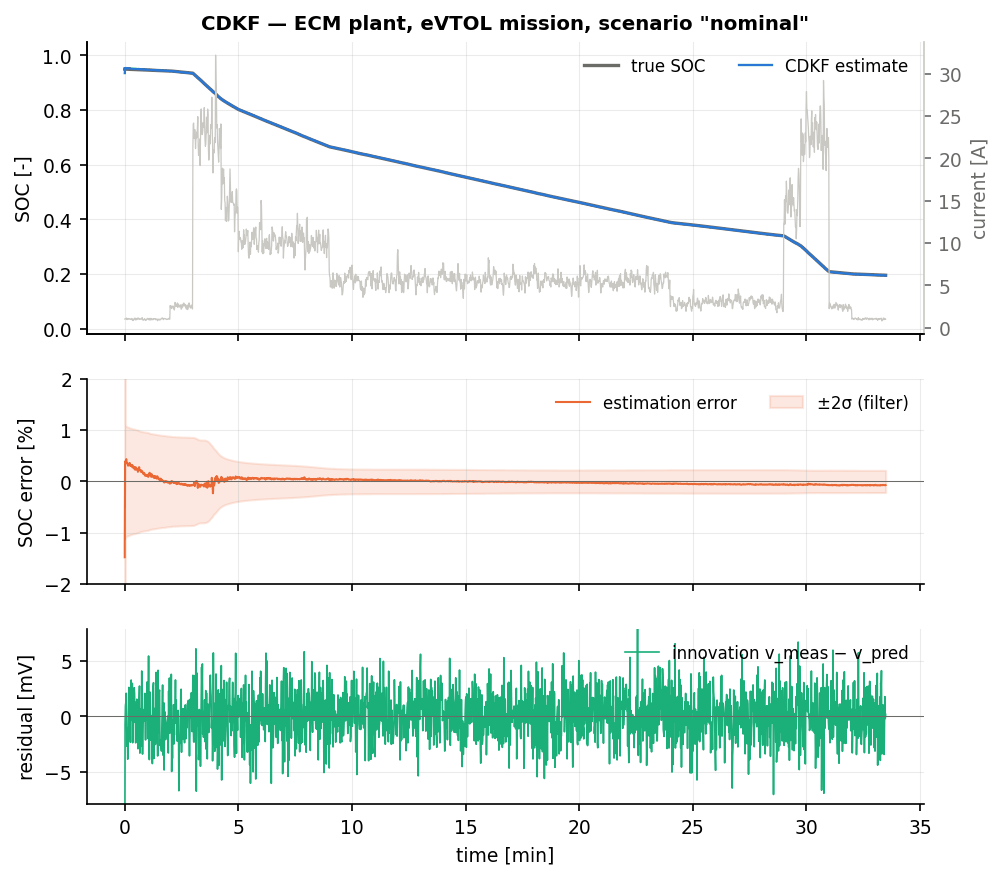
\includegraphics[width=\textwidth]{figures/cell_CDKF_nominal.png}
\caption{CDKF on the nominal eVTOL mission: true and estimated SOC (top), estimation error with the $\pm 2\sigma$ band when available (middle), voltage residual (bottom).}
\end{figure}
\begin{figure}[H]\centering
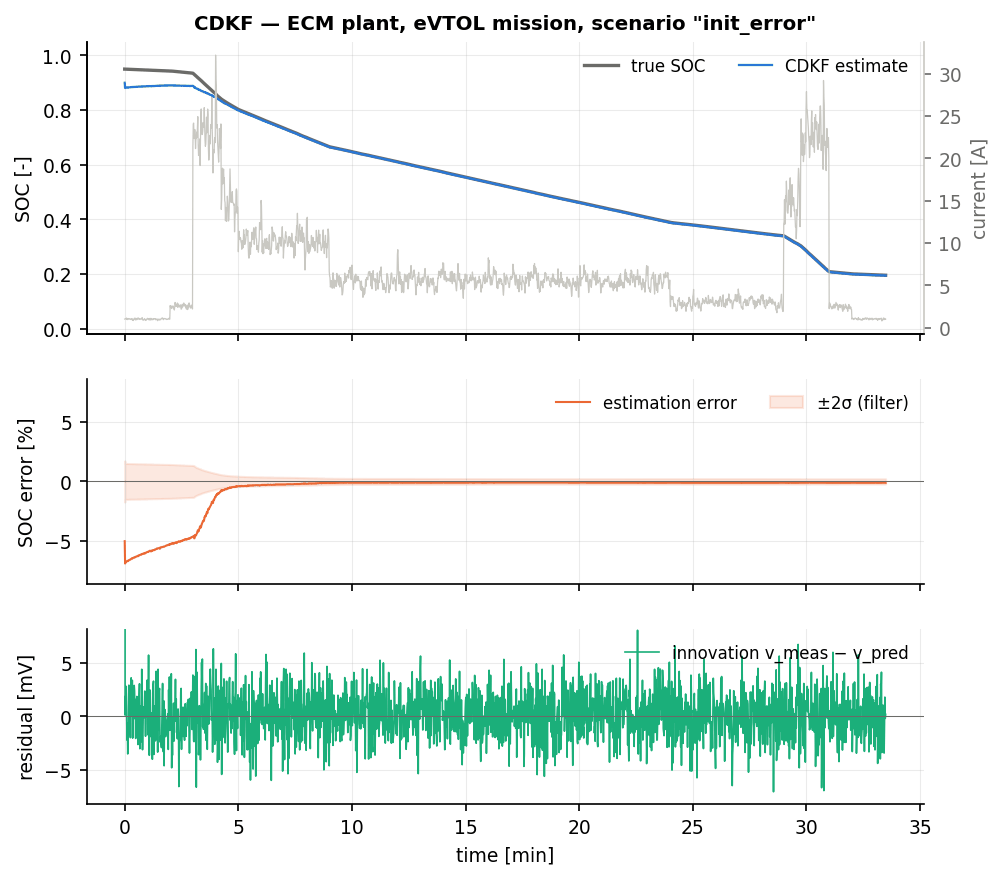
\includegraphics[width=\textwidth]{figures/cell_CDKF_init_error.png}
\caption{CDKF with a 35\,\% initial SOC error.}
\end{figure}

All numbers are three-seed means in per cent SOC.

The CDKF reproduces the fifth-degree cubature filter (Chapter~\ref{ch:ckf5}) and the $3$-point
Gauss--Hermite filter (Chapter~\ref{ch:ghkf}) to two decimals on all twelve ECM scenarios and
all nine SPM scenarios, which is the expected consequence of the three rules sharing the same
degree of exactness and, at $h^2 = 3$, essentially the same nodes. It does so with $9$ model
evaluations per stage instead of $33$ or $81$, and is therefore the \textbf{cheapest way to
obtain fifth-degree accuracy on this problem}: $1.28$--$1.39\,\SI{}{\micro\second}$ per step
against $3.7$--$4.1$ for the CKF5 and $11.2$--$12.1$ for the GHKF. That is the single most
useful practical finding of this group of chapters.

Numerically: \texttt{nominal} $0.08/0.05\,\%$ --- the equal-best whole-run RMSE of the family,
with the CKF and the two other fifth-degree rules, and better than the EKF's $0.15/0.05\,\%$
and the UKF's $0.20/0.04\,\%$; \texttt{outliers} $0.31/0.08\,\%$ with immediate convergence;
\texttt{aged\_cell} $2.50/1.54\,\%$ against the third-degree CKF's $2.87/1.79\,\%$;
\texttt{cold} $0.16/0.09\,\%$ and \texttt{hot} $0.08/0.04\,\%$, both better than the EKF's;
\texttt{current\_bias} $0.48/0.55\,\%$ against the EKF's $0.54/0.61\,\%$.

The weaknesses are those of every wide-stencil rule. \texttt{init\_error} takes $229$\,s to
converge with a whole-run RMSE of $1.85\,\%$ (steady state $0.12\,\%$), because with
$\sigma_\soc = 0.1$ the stencil reaches $\pm0.17$ SOC and the interpolating polynomial is a
poor model of the OCV over that range --- the same chord effect analysed in
Chapter~\ref{ch:ckf}. \texttt{sensor\_dropout} ($2.75/1.86\,\%$ against the EKF's
$0.72/0.46\,\%$) and \texttt{preisach} ($t_{\text{conv}} = 217$\,s against the EKF's $16$\,s)
are the same weakness seen through a fault and a bias. \texttt{param\_mismatch}
($1.84/1.79\,\%$) and \texttt{combined} ($14.64/11.96\,\%$, never converges) are model-error
scenarios where the extra integration accuracy is applied to the wrong model and does not help;
on \texttt{combined} the CDKF fails exactly as the EKF and CKF do, and for the same reason
(collapse of $\Pplus$ after the first update followed by an unmodelled $25\,\%$ rise in $R_0$).

\paragraph{SPM plant: structured model error.}
\begin{figure}[H]\centering
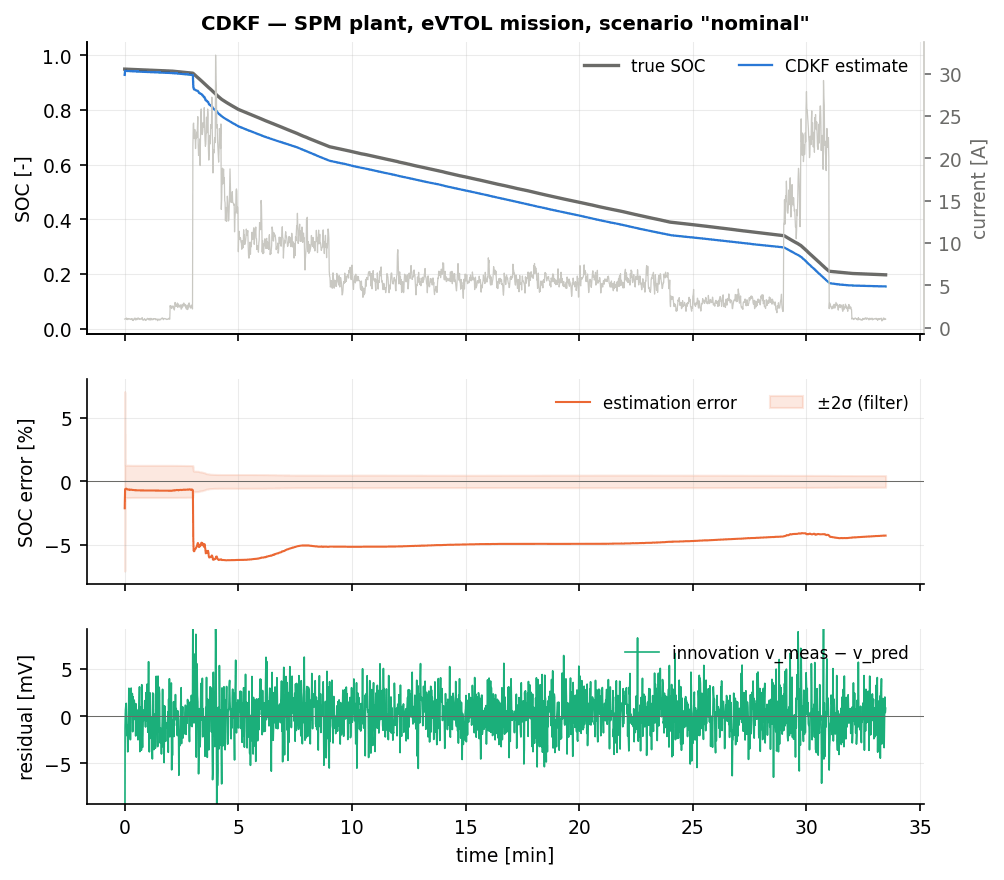
\includegraphics[width=\textwidth]{figures/cellspm_CDKF_nominal.png}
\caption{CDKF on the nominal mission with the electrochemical (SPM) plant.}
\end{figure}
The SPM block of the table is a different kind of test. The plant is the electrochemical
single-particle model; the estimator still runs a 2-RC equivalent circuit, fitted to that plant,
which leaves a \emph{structured} residual of about $4$\,mV (Butler--Volmer kinetics and
solid-phase diffusion that no 2-RC circuit can reproduce) and a slow second branch,
$\tau_2 = 556$\,s. Over a $33$-minute mission a $556$\,s pole barely relaxes, so $v_2(t)$ is
close to an affine ramp --- and so is $\ocv(\soc(t))$ while the cell discharges at a roughly
constant rate. The two channels through which the measurement sees the state,
$(\partial\ocv/\partial\soc)\,\delta\soc$ and $-\delta v_2$, are therefore nearly collinear in
the information accumulated over the flight: the pair $(\soc, v_2)$ is close to unobservable,
and no filter can decide whether a persistent few-millivolt residual belongs to the slow RC
branch or to the state of charge. Because that direction is weakly observable, a $4$\,mV
structured error maps onto \emph{several per cent} of SOC instead of the
$4\,\text{mV}/0.8\,\text{V}\approx0.5\,\%$ a well-conditioned channel would give. This
$(\soc,v_2)$ ambiguity, not the size of the residual, is the mechanism behind the
$3.7$--$4.6\,\%$ band in which the whole classical family sits.

The fifth-degree rules sit at the bad end of the band: $4.61\,\%$ on SPM \texttt{nominal}
against the EKF's $3.73\,\%$ and the LKF's $1.72\,\%$, $8.74\,\%$ on \texttt{cold} against
$7.35\,\%$, $8.24\,\%$ on \texttt{sensor\_dropout} against $5.31\,\%$, $4.90\,\%$ on
\texttt{param\_mismatch} against $3.13\,\%$. They are statistically indistinguishable from the
third-degree CKF ($4.62$, $8.72$, $8.24$, $4.81\,\%$) --- the extra degree of exactness buys
nothing at all here --- and the ordering across the family is monotone in the point spread:
LKF (frozen tangent) $1.72$, EKF/IEKF (tangent at the mean) $3.66$--$3.73$, UKF
($0.2\sigma$ points) $3.96$, the degree-three and degree-five rules ($2\sigma$ and
$2.45\sigma$) $4.61$--$4.62$. The reason is the ambiguity above: a statistical linearisation
over a wide prior returns the \emph{chord} of the OCV curve, which is steeper than the tangent
over most of the mission, so these filters believe the OCV channel is more informative than it
is and commit harder to the direction that carries the structured error. The exception is
\texttt{outliers} ($2.27\,\%$), better than on the ECM plant for everyone because the corrupted
samples widen the effective innovation covariance. Nothing diverges; every SPM error is a bias,
not a drift ($t_{\text{conv}} = 0$ throughout).

One point is specific to the divided-difference construction. On the ECM plant its second
difference is self-scaling: at $\sigma_\soc\approx10^{-3}$ the stencil shrinks below the OCV
table spacing and the $\mD^{(2)}$ term correctly vanishes, so the filter degenerates to an EKF
exactly when the EKF is right. On the SPM plant $\sigma_\soc$ stays large --- the filter is
never confident, because the residual keeps re-inflating it --- so the stencil stays wide and
the chord effect is permanently active. Self-scaling is a virtue when the covariance is
trustworthy and a liability when a structural residual keeps it open.

\section{Summary}
The DD2/CDKF is the best accuracy-per-flop sigma-point filter in this family: $9$ model
evaluations per stage buy fifth-degree moment accuracy, identical to a $33$-point cubature rule
or an $81$-point quadrature grid, and its second-difference term scales itself with $\mP$ so
that it disappears when the prior is tight. Use it as the default derivative-free filter,
particularly when analytic Jacobians are unavailable or when the measurement function is a
table. Its one parameter, $h$, should be left at $\sqrt3$ unless the function has a feature
narrower than $\sqrt3\sigma$; and like every wide-stencil method it converges slowly from a very
wide prior and is at the bad end of the family under structured model error, where an EKF or an
IEKF step is preferable.

% Copyright 2026 Sreeram Anil
% SPDX-License-Identifier: CC-BY-4.0
% =============================================================================
%  Gauss-Hermite quadrature Kalman filter — classical Kalman family
% =============================================================================
\chapter{Gauss--Hermite Quadrature Kalman Filter (GHKF)}
\label{ch:ghkf}

\section*{At a glance}
\begin{tabular}{@{}l>{\raggedright\arraybackslash}p{0.76\textwidth}@{}}
Family & classical Kalman (quadrature) \\
Header & \texttt{include/estkit/filters/ghkf.hpp} \\
Registered name & \texttt{GHKF} \\
State dimension & $n_x = 4$ (cell model) --- generic in $n_x, n_u, n_y$ \\
Quadrature points & $m^{n_x} = 3^4 = 81$ (points per axis $m$ is a template parameter) \\
Cost per step & $\mathcal{O}(m^{n_x} n_x^2)$; $11.2$--$12.1\,\SI{}{\micro\second}$/step \\
Primary references & \cite{ito2000gaussian,arasaratnam2007ghqf,wu2006numerical,golubwelsch1969} \\
\end{tabular}

\section{Motivation and aerospace/BMS relevance}
Every filter in this family is an approximation of the same Gaussian-weighted integral
\eqref{eq:ckf-integral}. The unscented, cubature and divided-difference rules all pick a
small, clever point set. The Gauss--Hermite filter of Ito and Xiong~\cite{ito2000gaussian}
instead uses the \emph{optimal} one-dimensional quadrature rule and forms a tensor product:
$m$ points per axis integrate polynomials of degree $\le 2m-1$ exactly, and the accuracy can
be dialled up simply by increasing $m$. It is therefore the natural reference implementation
of a Gaussian filter --- the estimator you run to find out how much of the remaining error is
due to the moment approximation and how much is due to the Gaussian assumption itself.

Its weakness is equally clear: the number of points grows as $m^{n_x}$. For the cell model
($n_x = 4$, $m = 3$) that is $81$ points, which is affordable; for a pack-level or
joint state-parameter model with $n_x = 10$ it would be $59\,049$ and the filter is unusable.
Sparse-grid and pruned variants exist, but the honest role of the GHKF in this report is as a
high-accuracy yardstick against which the $8$-, $9$- and $33$-point rules can be judged.

\section{Problem statement and assumptions}
Model \eqref{eq:ekf-proc}--\eqref{eq:ekf-meas} with additive noise; Gaussian assumed density;
the integrals of interest are \eqref{eq:ckf-integral}. The one additional structural
assumption is that $\mP$ admits a Cholesky factor $\mS$, used to decorrelate the coordinates
so that the $n_x$-dimensional Gaussian factorises into $n_x$ independent standard normals.

\section{Derivation}
\paragraph{One-dimensional rule.} The $m$-point Gauss--Hermite rule for the standard normal
weight is characterised by: nodes $\zeta_1,\dots,\zeta_m$ = roots of the $m$-th probabilists'
Hermite polynomial $He_m$, weights $\omega_j$ chosen so that
\begin{equation}
\int_{\real}\phi(\zeta)\,\frac{e^{-\zeta^2/2}}{\sqrt{2\pi}}\,d\zeta = \sum_{j=1}^m \omega_j\,\phi(\zeta_j)
\qquad\text{exactly for all polynomials } \phi \text{ of degree} \le 2m-1.
\label{eq:ghkf-1d}
\end{equation}
Nodes and weights are the eigenvalues and squared first eigenvector components of the
symmetric tridiagonal Jacobi matrix of the Hermite recurrence (Golub and
Welsch~\cite{golubwelsch1969}); for small $m$ they are available in closed form. For $m=3$,
$He_3(\zeta) = \zeta^3-3\zeta$, so
\begin{equation}
\zeta \in \left\{-\sqrt3,\;0,\;+\sqrt3\right\}, \qquad
\omega \in \left\{\tfrac16,\;\tfrac23,\;\tfrac16\right\}.
\label{eq:ghkf-m3}
\end{equation}
Checking the moments: $\sum\omega_j = 1$, $\sum\omega_j\zeta_j^2 = 2\cdot\tfrac16\cdot3 = 1$,
$\sum\omega_j\zeta_j^4 = 2\cdot\tfrac16\cdot9 = 3$ --- the first three even moments of
$\N{0}{1}$ are exact, and the first failure is at degree six
($\sum\omega_j\zeta_j^6 = 9$ against the true $15$), consistent with exactness to degree
$2m-1=5$. The $m=2$ rule, also tabulated in the header, has nodes $\pm1$ and weights
$\tfrac12$ and is exact to degree three --- it is the one-dimensional ancestor of the
third-degree cubature rule.

\paragraph{Tensor product.} With $\vx = \xhat + \mS\vz$ and $\vz\sim\N{\bm0}{\mI}$, the
$n_x$-dimensional integral factorises and the product rule is
\begin{equation}
\int g(\vx)\N{\vx;\xhat}{\mP}\,d\vx \approx
\sum_{j_1=1}^{m}\cdots\sum_{j_{n_x}=1}^{m}
\left(\prod_{r=1}^{n_x}\omega_{j_r}\right)
g\!\left(\xhat + \mS\,[\zeta_{j_1},\dots,\zeta_{j_{n_x}}]^\T\right),
\label{eq:ghkf-tensor}
\end{equation}
i.e. $N_s = m^{n_x}$ points $\bm{\xi}_s$ with weights $w_s = \prod_r \omega_{j_r}$, all
strictly positive. Because \eqref{eq:ghkf-1d} is exact per axis, \eqref{eq:ghkf-tensor} is
exact for every \emph{multivariate} polynomial whose degree in each individual variable is at
most $2m-1$ --- a stronger statement than the total-degree exactness of the cubature rules,
which is why a $3$-point grid matches a fifth-degree cubature rule and exceeds it on
cross-terms such as $z_1^4z_2^4$.

\paragraph{Filter recursion.} Identical in structure to the CKF, with the equal weights
replaced by $w_s$:
\begin{align}
\mathcal{X}_s &= \xhat + \mS\bm{\xi}_s, &
\xminus_k &= \sum_s w_s f(\mathcal{X}_s,\vu_{k-1}), \label{eq:ghkf-tu1}\\
\Pminus_k &= \sum_s w_s\left(f(\mathcal{X}_s,\vu_{k-1})-\xminus_k\right)(\cdot)^\T + \mQ, &&
\label{eq:ghkf-tu2}
\end{align}
and, after regenerating the grid from $(\xminus_k,\Pminus_k)$,
\begin{align}
\yhat_k &= \sum_s w_s\,h(\mathcal{X}_s,\vu_k), &
\mP_{yy} &= \sum_s w_s(\mathcal{Z}_s-\yhat_k)(\cdot)^\T + \mR, \label{eq:ghkf-mu1}\\
\mP_{xy} &= \sum_s w_s(\mathcal{X}_s-\xminus_k)(\mathcal{Z}_s-\yhat_k)^\T, &
\mK_k &= \mP_{xy}\mP_{yy}\inv, \label{eq:ghkf-mu2}
\end{align}
with $\xplus_k = \xminus_k + \mK_k(\vy_k-\yhat_k)$ and
$\Pplus_k = \Pminus_k - \mK_k\mP_{yy}\mK_k^\T$. Since all $w_s>0$, $\Pminus_k$ and the
subtracted term are both proper covariances and no definiteness safeguard beyond the usual
symmetrisation is needed.

\section{Algorithm}
\begin{algorithm}[H]
\caption{GHKF --- one sampling period (additive noise)}
\begin{algorithmic}[1]
\Require $\xplus_{k-1},\Pplus_{k-1},\vu_{k-1},\vy_k,\vu_k$; grid $\{\bm{\xi}_s,w_s\}_{s=1}^{m^{n_x}}$ precomputed
\State $\mS\gets\operatorname{chol}(\Pplus_{k-1})$;\; $\mathcal{X}_s\gets\xplus_{k-1}+\mS\bm{\xi}_s$
\State \textbf{Time update:} $\mathcal{X}_s\gets f(\mathcal{X}_s,\vu_{k-1})$;\;
       $\xminus_k\gets\sum_s w_s\mathcal{X}_s$;\;
       $\Pminus_k\gets\sum_s w_s(\mathcal{X}_s-\xminus_k)(\cdot)^\T+\mQ$
\State $\mS\gets\operatorname{chol}(\Pminus_k)$;\; $\mathcal{X}_s\gets\xminus_k+\mS\bm{\xi}_s$;\;
       $\mathcal{Z}_s\gets h(\mathcal{X}_s,\vu_k)$;\; $\yhat_k\gets\sum_s w_s\mathcal{Z}_s$
\State $\mP_{yy}\gets\sum_s w_s(\mathcal{Z}_s-\yhat_k)(\cdot)^\T+\mR$;\;
       $\mP_{xy}\gets\sum_s w_s(\mathcal{X}_s-\xminus_k)(\mathcal{Z}_s-\yhat_k)^\T$
\State $\mK\gets\mP_{xy}\mP_{yy}\inv$;\; $\xplus_k\gets\xminus_k+\mK(\vy_k-\yhat_k)$;\;
       $\Pplus_k\gets\Pminus_k-\mK\mP_{yy}\mK^\T$
\State \textbf{if} constraints enabled \textbf{then} $\xplus_k\gets\Pi(\xplus_k)$
\Ensure $\xplus_k,\Pplus_k$
\end{algorithmic}
\end{algorithm}

\section{Application to the battery model}
With $n_x=4$ and $m=3$ the grid has $81$ points. Of these, $16$ have all four coordinates at
$\pm\sqrt3$ (weight $1/1296$ each), $32$ have three (weight $1/324$), $24$ have two
(weight $1/81$), $8$ have one (weight $4/81$) and one is the mean (weight $16/81$). The
SOC axis is therefore sampled at $\soc$ and $\soc\pm\sqrt3\sigma_\soc$, the same stencil as
the DD2 filter of Chapter~\ref{ch:cdkf} --- which is exactly why the two produce identical
results on this problem.

Implementation choice: the number of points per axis is a template parameter,
\code{Ghkf<Model, MPTS>}, with compile-time node/weight tables for $m=2$ and $m=3$ and a
\code{static\_assert} otherwise, plus a second \code{static\_assert} that rejects grids above
$4096$ points. The registered estimator uses \code{Ghkf<EcmModel, 3>}. The grid itself
(abscissae $\bm{\xi}_s$ and weights $w_s$) is built once in the constructor by a mixed-radix
expansion of the grid index and stored as members, so the per-step work is only the affine map
$\xhat + \mS\bm{\xi}_s$ and the model evaluations.

\section{Implementation notes}
$162$ model evaluations per step is the entire cost story: at
$11.2$--$12.1\,\SI{}{\micro\second}$ per step the GHKF is $25\times$ an EKF step and $9\times$ a
CDKF step for identical accuracy.
Zero-coordinate axes are skipped in the affine map (a point with $\xi_r = 0$ contributes
nothing from column $r$ of $\mS$), which saves about a third of the multiply-accumulates in
the point generation. \code{sizeof(Ghkf<EcmModel,3>)} is 10\,784\,bytes --- by far the largest
in this family --- because the $81\times4$ abscissa table, the $81$ weights and the $81$
propagated points are all members; on a memory-constrained MCU this alone rules the filter
out. All weights are positive, so the single-precision build is unproblematic (measured
nominal $\text{RMSE}_{\text{ss}} = 0.02\,\%$ in float against $0.05\,\%$ in double, and
$1.96\,\%$ against $1.84\,\%$ on \texttt{aged\_cell} --- differences at the level of the noise
realisation rather than systematic).

\section{Benchmark results}
\input{tables/cell_GHKF.tex}
\begin{figure}[H]\centering
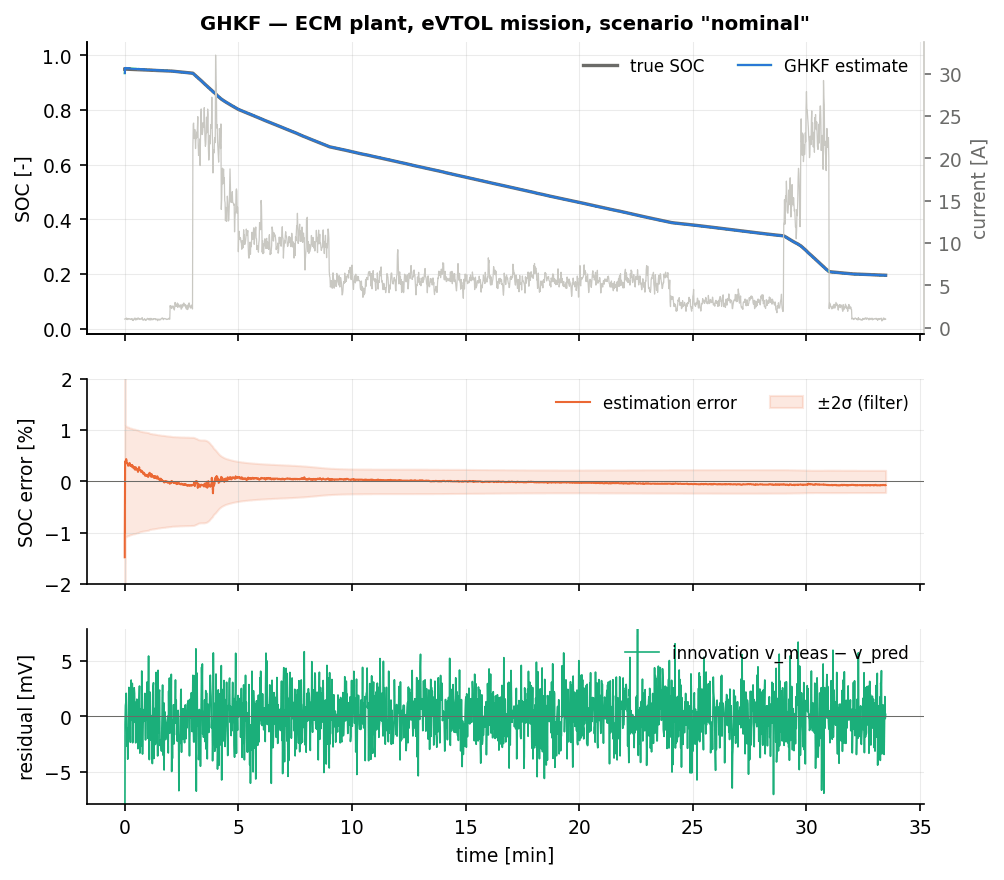
\includegraphics[width=\textwidth]{figures/cell_GHKF_nominal.png}
\caption{GHKF on the nominal eVTOL mission: true and estimated SOC (top), estimation error with the $\pm 2\sigma$ band when available (middle), voltage residual (bottom).}
\end{figure}
\begin{figure}[H]\centering
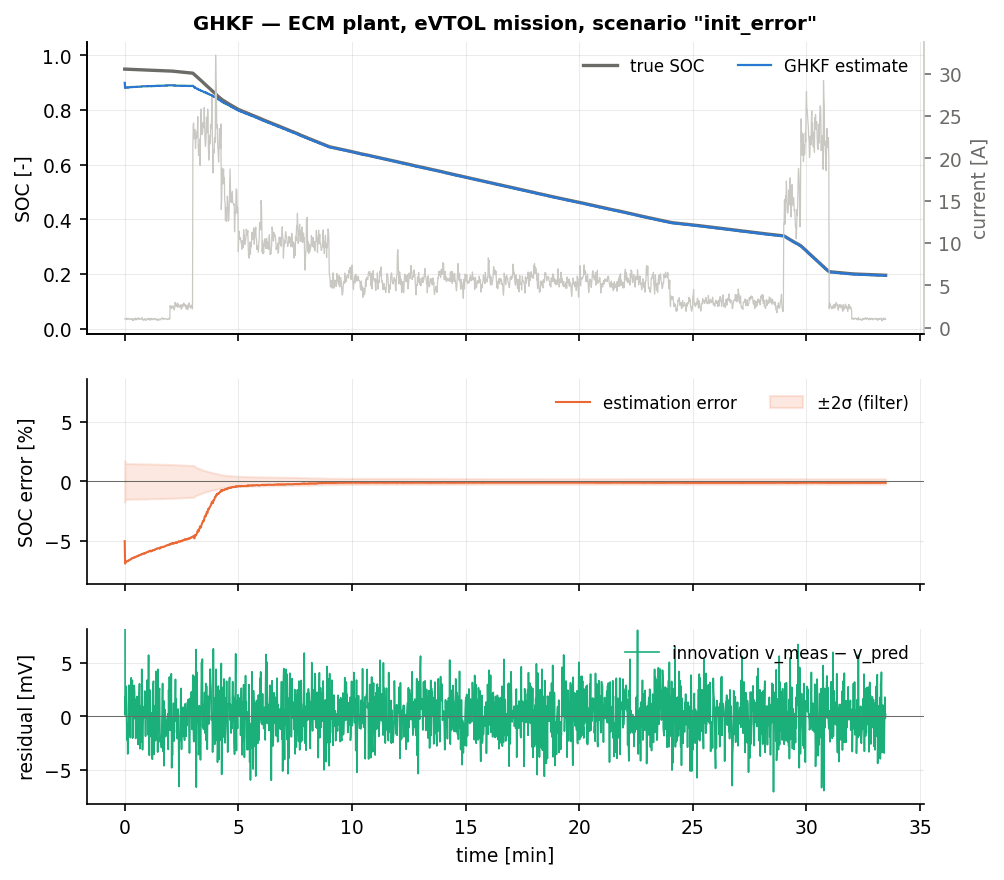
\includegraphics[width=\textwidth]{figures/cell_GHKF_init_error.png}
\caption{GHKF with a 35\,\% initial SOC error.}
\end{figure}

All numbers are three-seed means in per cent SOC.

The GHKF reproduces the CKF5 (Chapter~\ref{ch:ckf5}) and the CDKF (Chapter~\ref{ch:cdkf}) to two
decimal places on all twelve ECM scenarios and all nine SPM scenarios: \texttt{nominal}
$0.08/0.05\,\%$, \texttt{init\_error} $1.85/0.12\,\%$ with $t_{\text{conv}} = 229$\,s,
\texttt{outliers} $0.31/0.08\,\%$, \texttt{aged\_cell} $2.50/1.54\,\%$,
\texttt{param\_mismatch} $1.84/1.79\,\%$, \texttt{sensor\_dropout} $2.75/1.86\,\%$,
\texttt{preisach} $1.27/0.24\,\%$, \texttt{combined} $14.64/11.96\,\%$; SPM \texttt{nominal}
$4.70/4.61\,\%$ and \texttt{cold} $8.74\,\%$. Since the GHKF is the most accurate quadrature of
the three, this agreement is the strongest statement this report can make about the cell
problem: \textbf{beyond fifth-degree exactness there is nothing left to gain from better moment
integration}. Whatever error remains is due to the Gaussian assumption or to model error, not to
the quadrature; a particle filter or a Gaussian-sum filter, not a better cubature rule, would be
the next step.

The corollary is a cost statement. The GHKF pays $11.2$--$12.1\,\SI{}{\micro\second}$ per step
and $10.8$\,kB of state for results that the $9$-point DD2 filter obtains in
$1.28$--$1.39\,\SI{}{\micro\second}$ and $4.3$\,kB --- a factor of nine in time and two and a
half in memory. On this model there is no operating regime in which the GHKF is the right
engineering choice; its value here is diagnostic. That conclusion is specific to $n_x = 4$ and a
mildly nonlinear measurement --- in problems where $g$ has features narrower than $\sigma$,
raising $m$ is the only systematic way to resolve them, and the GHKF is then the only tool in
this chapter that can.

Like every wide-stencil rule it converges slowly from the $-35\,\%$ initial error ($229$\,s)
and from the hysteresis offset of \texttt{preisach} ($217$\,s against the EKF's $16$\,s), it is
well behind the EKF on \texttt{sensor\_dropout} ($1.86\,\%$ against $0.46\,\%$), and it fails
on \texttt{combined} ($11.96\,\%$, never converges) for the reason given in
Chapter~\ref{ch:ckf}: the posterior variance collapses after the first update and the estimate
is subsequently locked in against an unmodelled $25\,\%$ increase in $R_0$. Integrating a wrong
model very accurately does not make it right.

\paragraph{SPM plant: structured model error.}
\begin{figure}[H]\centering
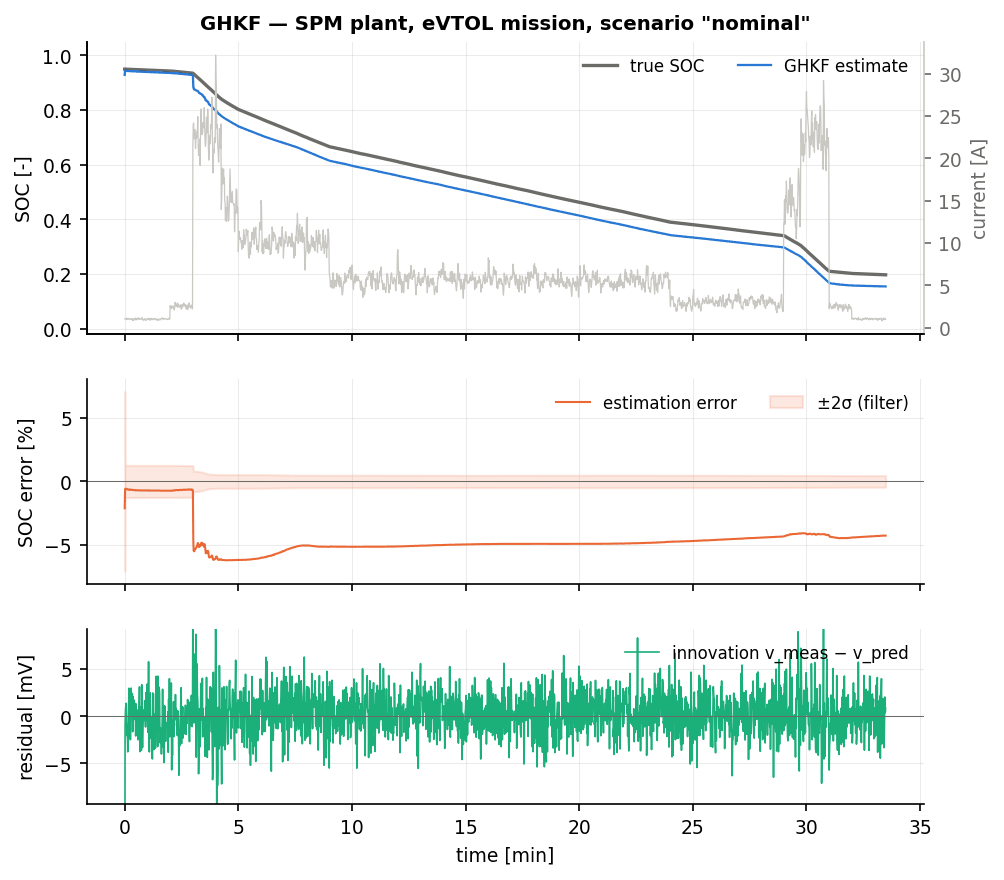
\includegraphics[width=\textwidth]{figures/cellspm_GHKF_nominal.png}
\caption{GHKF on the nominal mission with the electrochemical (SPM) plant.}
\end{figure}
The SPM block of the table is a different kind of test. The plant is the electrochemical
single-particle model; the estimator still runs a 2-RC equivalent circuit, fitted to that plant,
which leaves a \emph{structured} residual of about $4$\,mV (Butler--Volmer kinetics and
solid-phase diffusion that no 2-RC circuit can reproduce) and a slow second branch,
$\tau_2 = 556$\,s. Over a $33$-minute mission a $556$\,s pole barely relaxes, so $v_2(t)$ is
close to an affine ramp --- and so is $\ocv(\soc(t))$ while the cell discharges at a roughly
constant rate. The two channels through which the measurement sees the state,
$(\partial\ocv/\partial\soc)\,\delta\soc$ and $-\delta v_2$, are therefore nearly collinear in
the information accumulated over the flight: the pair $(\soc, v_2)$ is close to unobservable,
and no filter can decide whether a persistent few-millivolt residual belongs to the slow RC
branch or to the state of charge. Because that direction is weakly observable, a $4$\,mV
structured error maps onto \emph{several per cent} of SOC instead of the
$4\,\text{mV}/0.8\,\text{V}\approx0.5\,\%$ a well-conditioned channel would give. This
$(\soc,v_2)$ ambiguity, not the size of the residual, is the mechanism behind the
$3.7$--$4.6\,\%$ band in which the whole classical family sits.

The fifth-degree rules sit at the bad end of the band: $4.61\,\%$ on SPM \texttt{nominal}
against the EKF's $3.73\,\%$ and the LKF's $1.72\,\%$, $8.74\,\%$ on \texttt{cold} against
$7.35\,\%$, $8.24\,\%$ on \texttt{sensor\_dropout} against $5.31\,\%$, $4.90\,\%$ on
\texttt{param\_mismatch} against $3.13\,\%$. They are statistically indistinguishable from the
third-degree CKF ($4.62$, $8.72$, $8.24$, $4.81\,\%$) --- the extra degree of exactness buys
nothing at all here --- and the ordering across the family is monotone in the point spread:
LKF (frozen tangent) $1.72$, EKF/IEKF (tangent at the mean) $3.66$--$3.73$, UKF
($0.2\sigma$ points) $3.96$, the degree-three and degree-five rules ($2\sigma$ and
$2.45\sigma$) $4.61$--$4.62$. The reason is the ambiguity above: a statistical linearisation
over a wide prior returns the \emph{chord} of the OCV curve, which is steeper than the tangent
over most of the mission, so these filters believe the OCV channel is more informative than it
is and commit harder to the direction that carries the structured error. The exception is
\texttt{outliers} ($2.27\,\%$), better than on the ECM plant for everyone because the corrupted
samples widen the effective innovation covariance. Nothing diverges; every SPM error is a bias,
not a drift ($t_{\text{conv}} = 0$ throughout).

The SPM rows make the diagnostic point of this chapter unusually sharply. The GHKF integrates
the Gaussian moments essentially exactly, and it is still $4.6\,\%$ wrong --- worse than the
crudest filter in the family. That is the clearest possible demonstration that the residual
error on the SPM plant is \emph{not} quadrature error: it is the Gaussian assumption meeting a
mis-specified model along a nearly unobservable direction, and no amount of integration
accuracy touches it.

\section{Summary}
The Gauss--Hermite filter is the reference Gaussian filter: tensor-product quadrature, all
weights positive, accuracy set by a single integer $m$, and exactness to degree $2m-1$ in every
variable. Use it to establish how much of a filter's error is quadrature error --- on this
benchmark the answer is ``none beyond degree five'', on either plant --- or on genuinely hard,
strongly nonlinear low-dimensional problems where $m$ must be raised. Do not use it in
production at $n_x\gtrsim6$: $m^{n_x}$ points is a wall, and the DD2 filter of
Chapter~\ref{ch:cdkf} delivers identical results here at one ninth of the cost.

% Copyright 2026 Sreeram Anil
% SPDX-License-Identifier: CC-BY-4.0
% =============================================================================
%  Iterated posterior linearisation filter — classical Kalman family
% =============================================================================
\chapter{Iterated Posterior Linearisation Filter (IPLF)}
\label{ch:iplf}

\section*{At a glance}
\begin{tabular}{@{}l>{\raggedright\arraybackslash}p{0.76\textwidth}@{}}
Family & classical Kalman (sigma-point, iterated) \\
Header & \texttt{include/estkit/filters/iplf.hpp} \\
Registered name & \texttt{IPLF} \\
State dimension & $n_x = 4$ (cell model) --- generic in $n_x, n_u, n_y$ \\
Sigma points & $2n_x+1 = 9$ per iteration, $\le 5$ iterations \\
Cost per step & $\mathcal{O}(J n_x^3)$ plus $(J{+}1)(2n_x{+}1)$ model calls; $1.92$--$2.08\,\SI{}{\micro\second}$/step \\
Primary references & \cite{garciafernandez2015iplf,garciafernandez2017ipls,julier2000newmethod,bellcathey1993} \\
\end{tabular}

\section{Motivation and aerospace/BMS relevance}
Two ideas have appeared separately in this family. The sigma-point filters replace the
Jacobian by a \emph{statistical linear regression} (SLR) of $h$ taken with respect to the
\emph{prior}; the iterated EKF keeps the analytic Jacobian but moves the expansion point to
the \emph{posterior}. García-Fernández, Svensson, Morelande and
Särkkä~\cite{garciafernandez2015iplf} observed that the two are orthogonal improvements and
combined them: perform the SLR with respect to the current posterior approximation and
iterate.

The argument for doing so is precise. The best linear approximation of $h$ in a mean-square
sense depends on the density with respect to which the error is measured. A filter should
linearise where the state actually \emph{is} (the posterior), not where it was believed to be
before the measurement (the prior). When the measurement is informative --- and a battery
terminal-voltage measurement with $\sigma_v = 2$\,mV against an OCV slope of $0.8$\,V is very
informative --- the posterior is far narrower than the prior, and a regression over the
prior wastes its accuracy on regions of the state space the measurement has just excluded.

For BMS the practical case is again initialisation and fault recovery, and for GNC it is the
classic one of a very accurate sensor with a nonlinear model (range, bearing, star tracker).

\section{Problem statement and assumptions}
Model \eqref{eq:ekf-proc}--\eqref{eq:ekf-meas}, additive noise. Given a Gaussian prior
$\N{\xminus_k}{\Pminus_k}$ and a measurement $\vy_k$, the goal is the Gaussian
$\N{\vx_J}{\mP_J}$ that best approximates the true posterior in Kullback--Leibler divergence.
The filter assumes a Gaussian posterior; it makes no differentiability assumption on $h$.

\begin{definition}[Statistical linear regression]\label{def:slr}
Given a density $p(\vx)$ with mean $\bar\vx$ and covariance $\bar\mP$, the SLR of $h$ with
respect to $p$ is the triple $(\mA,\bm{b},\bm{\Omega})$ minimising
$\E{\norm{h(\vx)-(\mA\vx+\bm{b})}^2}$ under $p$, together with the covariance
$\bm{\Omega}$ of the residual $h(\vx)-(\mA\vx+\bm b)$.
\end{definition}

\section{Derivation}
\paragraph{Closed form of the SLR.} Writing
$\bar{\vy} = \E{h(\vx)}$, $\bm{\Psi} = \E{(\vx-\bar\vx)(h(\vx)-\bar\vy)^\T}$ and
$\bm{\Phi} = \E{(h(\vx)-\bar\vy)(h(\vx)-\bar\vy)^\T}$, the first-order conditions of the
least-squares problem in Definition~\ref{def:slr} give
\begin{equation}
\mA = \bm{\Psi}^\T\bar{\mP}\inv, \qquad
\bm{b} = \bar{\vy} - \mA\bar{\vx}, \qquad
\bm{\Omega} = \bm{\Phi} - \mA\bar{\mP}\mA^\T,
\label{eq:iplf-slr}
\end{equation}
with $\bm{\Omega}\succeq 0$ by construction (it is the covariance of the part of $h$ that no
affine function of $\vx$ can explain). The three moments $\bar\vy,\bm\Psi,\bm\Phi$ are
evaluated with the sigma-point rule of Chapter~\ref{ch:ukf}; any of the rules in this family
would do.

\paragraph{The iteration.} Initialise $\vx_0 = \xminus_k$, $\mP_0 = \Pminus_k$. For
$j=0,1,\dots$: compute the SLR $(\mA_j,\bm b_j,\bm\Omega_j)$ of $h$ with respect to
$\N{\vx_j}{\mP_j}$ using \eqref{eq:iplf-slr}, then update the \emph{prior} with the resulting
affine measurement model $\vy = \mA_j\vx + \bm b_j + \bm{e}$,
$\bm{e}\sim\N{\bm0}{\bm\Omega_j + \mR}$:
\begin{align}
\mS_j &= \mA_j\Pminus_k\mA_j^\T + \bm\Omega_j + \mR, &
\mK_j &= \Pminus_k\mA_j^\T\mS_j\inv, \label{eq:iplf-gain}\\
\vx_{j+1} &= \xminus_k + \mK_j\left(\vy_k - \mA_j\xminus_k - \bm b_j\right), &
\mP_{j+1} &= \Pminus_k - \mK_j\mS_j\mK_j^\T. \label{eq:iplf-update}
\end{align}
It is essential that \eqref{eq:iplf-update} updates the \emph{original} prior
$(\xminus_k,\Pminus_k)$, not $(\vx_j,\mP_j)$: the iteration changes only where the
measurement model is linearised, never how much information has been used.

\begin{proposition}[One iteration is the sigma-point filter]\label{prop:iplf-first}
With $\vx_0 = \xminus_k$, $\mP_0=\Pminus_k$, \eqref{eq:iplf-gain}--\eqref{eq:iplf-update}
reduce exactly to the UKF measurement update \eqref{eq:ukf-pyy}--\eqref{eq:ukf-mu}.
\end{proposition}
\begin{proof}
With $\bar\mP = \Pminus_k$, $\bm\Omega_0 = \bm\Phi - \mA_0\Pminus_k\mA_0^\T$, hence
$\mS_0 = \bm\Phi + \mR = \mP_{yy}$. Also
$\mK_0 = \Pminus_k\mA_0^\T\mS_0\inv = \Pminus_k(\Pminus_k)\inv\bm\Psi\,\mP_{yy}\inv =
\mP_{xy}\mP_{yy}\inv$, and
$\vy_k - \mA_0\xminus_k-\bm b_0 = \vy_k - \bar\vy = \vy_k-\yhat_k$. Substituting gives
\eqref{eq:ukf-mu}.
\end{proof}
Proposition~\ref{prop:iplf-first} was verified numerically: with \code{max\_iter = 1} the IPLF
and the library UKF agree to $\max\abs{\Delta\vx} = 4.0\times10^{-11}$ over a full mission.

\paragraph{Interpretation and convergence.} García-Fernández et
al.~\cite{garciafernandez2015iplf} show that \eqref{eq:iplf-gain}--\eqref{eq:iplf-update} is a
fixed-point iteration whose fixed points are the stationary points of the KL divergence
between the true posterior and the Gaussian family, and that the IEKF
(Chapter~\ref{ch:iekf}) is recovered if the SLR in \eqref{eq:iplf-slr} is replaced by a Taylor
linearisation at $\vx_j$ --- the IPLF is the IEKF with derivatives replaced by regressions
and, crucially, with $\bm\Omega_j$ accounting for the part of $h$ that no linearisation can
capture. Convergence is not guaranteed in general; as with Gauss--Newton the practical
remedy is a small iteration budget, used here.

\section{Algorithm}
\begin{algorithm}[H]
\caption{IPLF --- one sampling period}
\begin{algorithmic}[1]
\Require $\xplus_{k-1},\Pplus_{k-1},\vu_{k-1},\vy_k,\vu_k$, $J_{\max}$, tolerance $\epsilon$
\State \textbf{Time update:} sigma-point prediction \eqref{eq:ukf-tu-mean}--\eqref{eq:ukf-tu-cov} $\Rightarrow (\xminus_k,\Pminus_k)$
\State $\vx_0\gets\xminus_k$, $\mP_0\gets\Pminus_k$
\For{$j=0,\dots,J_{\max}-1$}
  \State generate sigma points from $(\vx_j,\mP_j)$; $\mathcal{Z}_i\gets h(\mathcal{X}_i,\vu_k)$
  \State $\bar\vy\gets\sum_i W^m_i\mathcal{Z}_i$;\;
         $\bm\Psi\gets\sum_i W^c_i(\mathcal{X}_i-\vx_j)(\mathcal{Z}_i-\bar\vy)^\T$;\;
         $\bm\Phi\gets\sum_i W^c_i(\mathcal{Z}_i-\bar\vy)(\cdot)^\T$
  \State $\mA\gets\bm\Psi^\T\mP_j\inv$ (Cholesky solve);\; $\bm b\gets\bar\vy-\mA\vx_j$;\;
         $\bm\Omega\gets\bm\Phi-\mA\mP_j\mA^\T$, clipped to $\succeq0$
  \State $\mS\gets\mA\Pminus_k\mA^\T+\bm\Omega+\mR$;\; $\mK\gets\Pminus_k\mA^\T\mS\inv$
  \State $\vx_{j+1}\gets\xminus_k+\mK(\vy_k-\mA\xminus_k-\bm b)$;\;
         $\mP_{j+1}\gets\Pminus_k-\mK\mS\mK^\T$
  \State \textbf{if} $\norm{\vx_{j+1}-\vx_j}\le\epsilon(1+\norm{\vx_{j+1}})$ \textbf{then break}
\EndFor
\State $\xplus_k\gets\vx_J$, $\Pplus_k\gets\mP_J$;
       \textbf{if} constraints enabled \textbf{then} $\xplus_k\gets\Pi(\xplus_k)$
\Ensure $\xplus_k,\Pplus_k$
\end{algorithmic}
\end{algorithm}

\section{Application to the battery model}
The regression matrix $\mA$ has a direct physical reading here: its first entry is the
\emph{effective OCV slope} averaged over the current posterior. During the first iteration
that average is taken over the prior ($\sigma_\soc$ up to $0.1$ at start-up) and is the chord
of the OCV curve; by the second iteration the posterior is already $30\times$ narrower and
the regression returns essentially the local tangent --- so the IPLF automatically interpolates
between the CKF's chord behaviour and the EKF's tangent behaviour as the measurement takes
effect. This is the cleanest available answer to the trade-off identified in
Chapters~\ref{ch:ckf} and~\ref{ch:ekf}.

The residual covariance $\bm\Omega$ is the second useful quantity: it is the variance of the
OCV nonlinearity that the affine fit cannot explain, and it is added to $\mR$, so the filter
automatically de-weights the voltage measurement while the SOC uncertainty is large. That is
the same inflation that the UKF obtains accidentally through a large negative $W_0^c$
(Remark~\ref{rm:ukf-w0}) and the second-order EKF obtains explicitly
(Chapter~\ref{ch:soekf}), but here it is derived rather than incidental.

Options: $\alpha=0.1,\beta=2,\kappa=0$ (matching the UKF so that
Proposition~\ref{prop:iplf-first} can be checked), \code{max\_iter = 5},
\code{tol}$=10^{-6}$, \code{apply\_constraints = true}.

\section{Implementation notes}
$\mA = \bm\Psi^\T\mP_j\inv$ is computed as $(\,\code{solve\_spd}(\mP_j,\bm\Psi)\,)^\T$, never
by forming an explicit inverse; if the Cholesky solve fails the iteration breaks and the last
valid iterate is kept. $\bm\Omega$ is clipped to a non-negative diagonal and symmetrised,
which guards against the small negative values that sigma-point moment sums with negative
$W_0^c$ can produce. Sigma points are regenerated from $(\vx_j,\mP_j)$ at every iteration ---
that is the whole point of the algorithm --- so the cost is $(J+1)\times 9$ model
evaluations; the measured $1.92$--$2.08\,\SI{}{\micro\second}$ per step implies an average of
about two iterations. \code{sizeof(Iplf<EcmModel>)} is 4784\,bytes.

\section{Benchmark results}
% Copyright 2026 Sreeram Anil
% SPDX-License-Identifier: CC-BY-4.0
\begin{table}[H]\centering\footnotesize\setlength{\tabcolsep}{4pt}
\caption{IPLF: cell-level benchmark on the eVTOL mission (mean over seeds; RMSE and max error in \% SOC; $t_\mathrm{conv}$: first time the error stays below 2\,\% for 60\,s, -- = never; EKF reference: steady-state RMSE of the plain EKF on the same data).}\label{tab:cell_IPLF}
\begin{tabular}{llrrrrrcrr}\toprule
plant & scenario & RMSE & RMSE$_\mathrm{ss}$ & max & $t_\mathrm{conv}$ [s] & RMSE$_v$ [mV] & div. & EKF ref. & ns/step \\ \midrule
ECM & nominal & 0.36 & 0.08 & 3.57 & 0 & 1.09 & no & 0.05 & 2032 \\
ECM & init\_error & 0.32 & 0.07 & 1.17 & 0 & 2.05 & no & 0.05 & 2033 \\
ECM & current\_bias & 0.70 & 0.57 & 3.35 & 0 & 1.12 & no & 0.61 & 2042 \\
ECM & noise\_step & 0.39 & 0.19 & 3.57 & 0 & 2.98 & no & 0.12 & 2077 \\
ECM & outliers & 0.94 & 0.26 & 5.77 & 174 & 2.23 & no & 0.21 & 2025 \\
ECM & cold & 0.54 & 0.50 & 3.53 & 0 & 2.03 & no & 0.16 & 2041 \\
ECM & hot & 0.44 & 0.02 & 3.59 & 0 & 0.92 & no & 0.03 & 2040 \\
ECM & aged\_cell & 1.83 & 2.16 & 4.66 & 0 & 3.99 & no & 1.52 & 2050 \\
ECM & param\_mismatch & 0.65 & 0.53 & 4.65 & 0 & 2.95 & no & 1.36 & 2067 \\
ECM & sensor\_dropout & 1.27 & 0.79 & 4.22 & 0 & 1.89 & no & 0.46 & 2047 \\
ECM & preisach & 0.49 & 0.20 & 3.66 & 1 & 1.16 & no & 0.20 & 2058 \\
ECM & combined & 1.49 & 1.72 & 4.90 & 0 & 4.67 & no & 12.44 & 2078 \\
\midrule
SPM & nominal & 3.65 & 3.74 & 4.39 & 0 & 1.30 & no & 3.73 & 1946 \\
SPM & init\_error & 3.94 & 4.01 & 4.68 & 0 & 2.11 & no & 3.81 & 1920 \\
SPM & current\_bias & 5.56 & 6.31 & 7.16 & 0 & 1.37 & no & 5.69 & 1940 \\
SPM & noise\_step & 4.70 & 5.55 & 8.61 & 0 & 3.26 & no & 3.30 & 2003 \\
SPM & outliers & 1.38 & 1.02 & 4.77 & 70 & 2.44 & no & 1.99 & 1922 \\
SPM & cold & 7.19 & 7.54 & 9.99 & -- & 4.59 & no & 7.35 & 1939 \\
SPM & hot & 2.25 & 2.33 & 3.55 & 0 & 1.04 & no & 2.16 & 1933 \\
SPM & param\_mismatch & 3.38 & 3.68 & 4.27 & 0 & 2.12 & no & 3.13 & 1922 \\
SPM & sensor\_dropout & 6.07 & 6.30 & 6.80 & 0 & 2.09 & no & 5.31 & 1924 \\
\bottomrule\end{tabular}\end{table}

\begin{figure}[H]\centering
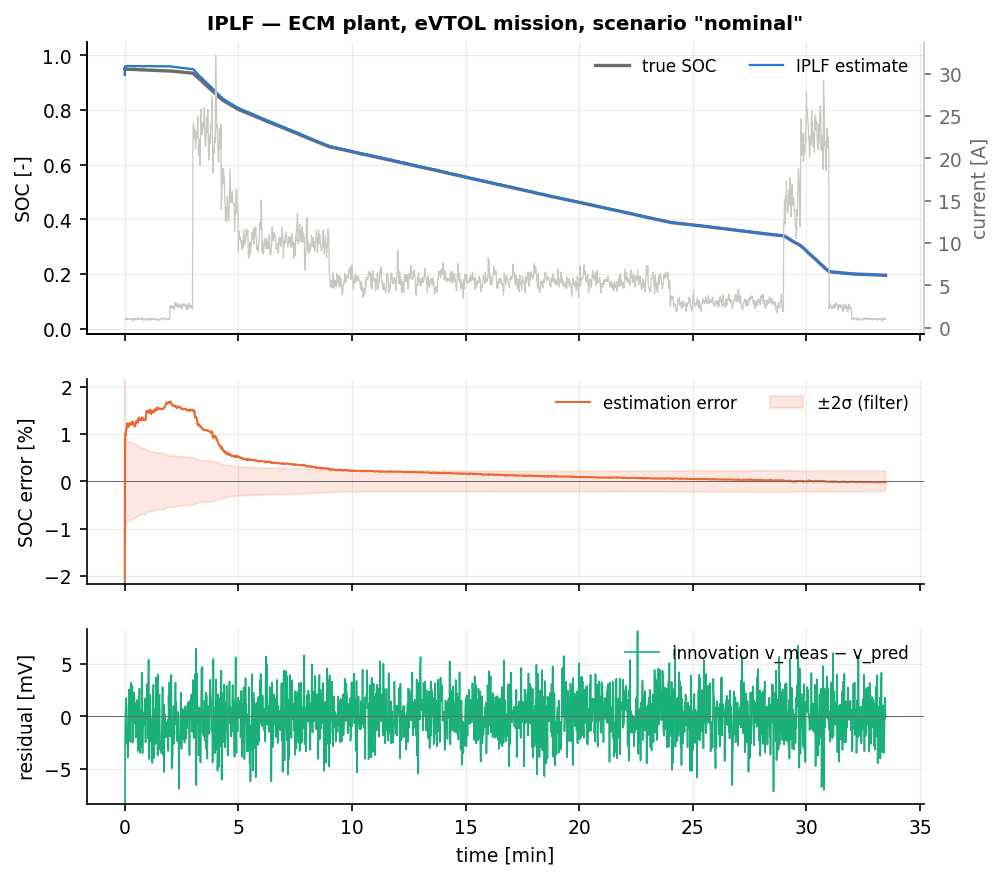
\includegraphics[width=\textwidth]{figures/cell_IPLF_nominal.png}
\caption{IPLF on the nominal eVTOL mission: true and estimated SOC (top), estimation error with the $\pm 2\sigma$ band when available (middle), voltage residual (bottom).}
\end{figure}
\begin{figure}[H]\centering
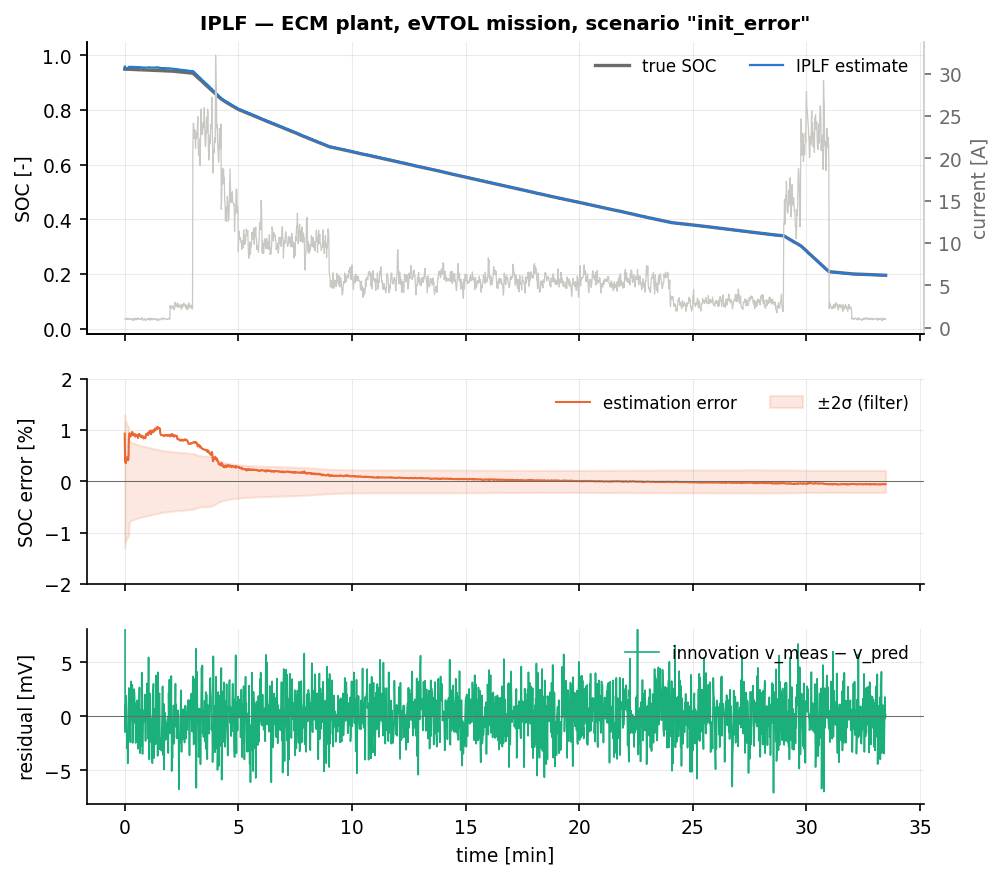
\includegraphics[width=\textwidth]{figures/cell_IPLF_init_error.png}
\caption{IPLF with a 35\,\% initial SOC error.}
\end{figure}
\begin{figure}[H]\centering
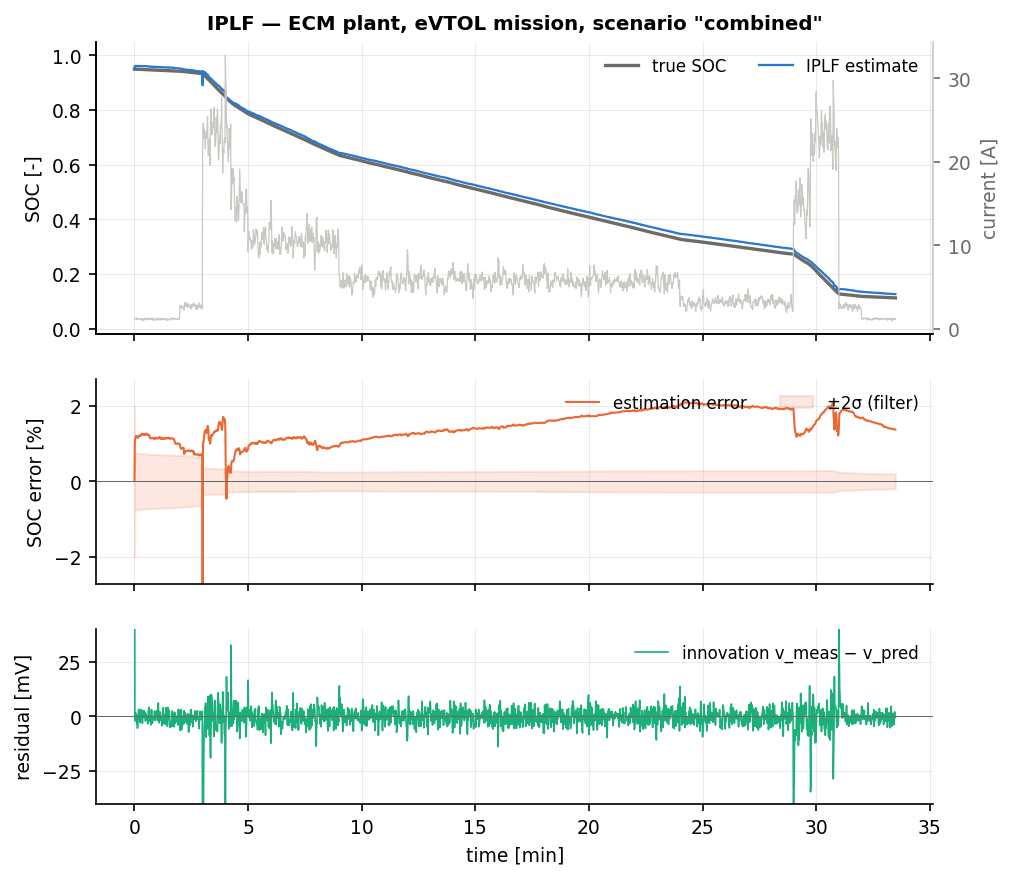
\includegraphics[width=\textwidth]{figures/cell_IPLF_combined.png}
\caption{IPLF on the \texttt{combined} scenario: the regression residual covariance $\bm\Omega$ de-weights the voltage while $\sigma_\soc$ is large, and the filter converges in the first sample.}
\end{figure}

All numbers are three-seed means in per cent SOC.

The IPLF has the best steady-state accuracy of any filter in the family on the two scenarios
that punish a bad linearisation hardest. \texttt{param\_mismatch} gives $0.65/0.53\,\%$ ---
the best of all fifteen, against the EKF's $1.28/1.36\,\%$, the UKF's $1.29/1.37\,\%$ and the
SO-EKF's $0.77/0.89\,\%$ --- and \texttt{hot} $0.02\,\%$, also the best. On \texttt{combined}
it converges in the first sample and reaches $1.49/1.72\,\%$, in the same class as the UKF
($1.19\,\%$) and the SO-EKF ($1.28\,\%$) and far better than the EKF ($12.44\,\%$); on
\texttt{init\_error} it converges immediately with $0.32/0.07\,\%$ where the CKF, CKF5, CDKF
and GHKF all need over $220$\,s. \texttt{preisach} is the fastest convergence of the fifteen
($1$\,s, against $16$\,s for the EKF and $214$--$229$\,s for the sigma-point filters) at
$0.49/0.20\,\%$ --- the regression absorbs the hysteresis offset immediately instead of
waiting for the covariance to reopen.

The whole-run RMSE on \texttt{nominal} ($0.36\,\%$ against the EKF's $0.15\,\%$, steady state
$0.08\,\%$ against $0.05\,\%$) and the convergence metric are the cost of that behaviour. In
the first seconds $\bm\Omega$ is large --- the OCV nonlinearity over $\sigma_\soc = 0.1$ is
genuinely un-modellable by an affine fit --- so the filter deliberately distrusts the first
voltage samples. That is correct behaviour, not a defect; the same caution is what makes
\texttt{combined} and \texttt{param\_mismatch} work.

Two clear regressions. \texttt{aged\_cell} is $1.83/2.16\,\%$ against the EKF's
$1.18/1.52\,\%$ and the CKF5's $2.50/1.54\,\%$ --- the worst steady-state figure of the family
apart from the LKF. With a $15\,\%$ capacity loss the model is simply wrong, the innovations
are persistently biased, and iterating the linearisation onto a posterior that is itself biased
reinforces the error. \texttt{cold} shows the same pattern on a smaller scale ($0.50\,\%$
against the UKF's $0.07\,\%$ and the EKF's $0.16\,\%$), as does \texttt{outliers}
($0.94/0.26\,\%$, with $t_{\text{conv}} = 174$\,s) --- fitting a corrupted measurement
\emph{better} is not an improvement, the same structural objection that applies to the IEKF.

Iteration-count sensitivity measured during development: $J = 1$ reproduces the UKF exactly,
$J = 2$ gives the best \texttt{combined} figure, and $J = 3,5,10$ are non-monotone. As with the
IEKF, more iterations is not monotonically better once model error dominates.

\paragraph{SPM plant: structured model error.}
\begin{figure}[H]\centering
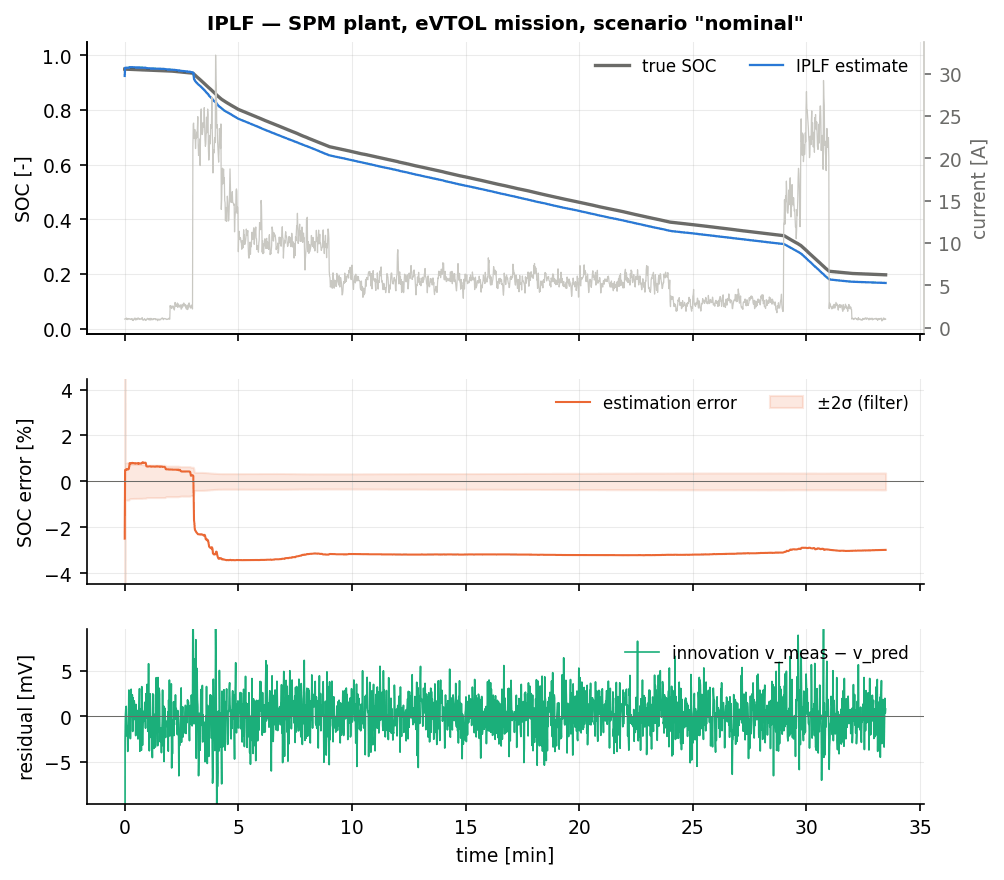
\includegraphics[width=\textwidth]{figures/cellspm_IPLF_nominal.png}
\caption{IPLF on the nominal mission with the electrochemical (SPM) plant.}
\end{figure}
The SPM block of the table is a different kind of test. The plant is the electrochemical
single-particle model; the estimator still runs a 2-RC equivalent circuit, fitted to that plant,
which leaves a \emph{structured} residual of about $4$\,mV (Butler--Volmer kinetics and
solid-phase diffusion that no 2-RC circuit can reproduce) and a slow second branch,
$\tau_2 = 556$\,s. Over a $33$-minute mission a $556$\,s pole barely relaxes, so $v_2(t)$ is
close to an affine ramp --- and so is $\ocv(\soc(t))$ while the cell discharges at a roughly
constant rate. The two channels through which the measurement sees the state,
$(\partial\ocv/\partial\soc)\,\delta\soc$ and $-\delta v_2$, are therefore nearly collinear in
the information accumulated over the flight: the pair $(\soc, v_2)$ is close to unobservable,
and no filter can decide whether a persistent few-millivolt residual belongs to the slow RC
branch or to the state of charge. Because that direction is weakly observable, a $4$\,mV
structured error maps onto \emph{several per cent} of SOC instead of the
$4\,\text{mV}/0.8\,\text{V}\approx0.5\,\%$ a well-conditioned channel would give. This
$(\soc,v_2)$ ambiguity, not the size of the residual, is the mechanism behind the
$3.7$--$4.6\,\%$ band in which the whole classical family sits.

The IPLF lands at $3.74\,\%$ on SPM \texttt{nominal}, essentially on top of the EKF's
$3.73\,\%$ and well ahead of the other sigma-point filters (UKF $3.96\,\%$, cubature family
$4.61$--$4.62\,\%$). That is the posterior linearisation doing what it is designed to do: after
the first iteration the regression is taken over a posterior that is $30\times$ narrower than
the prior, so the effective OCV slope is the local tangent rather than the chord, and the
filter does not over-weight the ill-conditioned channel the way a prior-based regression does.
It is the best SPM \texttt{outliers} result of the family by a wide margin ($1.02\,\%$ against
the EKF's $1.99\,\%$ and the cubature filters' $2.21$--$2.27\,\%$), because $\bm\Omega$ absorbs
exactly the part of the residual that no affine model explains.

What it does not do is escape the band. On \texttt{noise\_step} it is the worst of the fifteen
($5.55\,\%$ against the EKF's $3.30\,\%$): when the voltage noise steps up by an order of
magnitude the posterior stops being narrow, the regression widens again, and the filter
re-commits to the ambiguous direction. \texttt{sensor\_dropout} ($6.30\,\%$ against $5.31\,\%$)
and \texttt{current\_bias} ($6.31\,\%$ against $5.69\,\%$) show the same. Linearising in the
right place is worth about $6\,\%$ here; resolving the $(\soc,v_2)$ ambiguity would need an
extra state or a second sensor, not a better linearisation.

\section{Summary}
The IPLF is the most principled filter in this family: it linearises statistically, where the
state is, and it charges the linearisation residual $\bm\Omega$ to the measurement noise so
that the filter's confidence matches the quality of its own approximation. On this benchmark it
delivers the best steady-state accuracy on \texttt{param\_mismatch} and \texttt{hot}, the
fastest convergence on \texttt{preisach}, immediate convergence from a large initial error, and
it survives \texttt{combined}, at about $1.4\times$ the cost of a UKF. Use it when the
measurement is informative and strongly nonlinear. Do not expect it to help when the model
itself is biased --- on \texttt{aged\_cell} it is the worst of the sigma-point filters, and on
the SPM plant it merely matches the EKF --- because a better fit to a wrong model is still
wrong.

% Copyright 2026 Sreeram Anil
% SPDX-License-Identifier: CC-BY-4.0
% =============================================================================
%  Square-root extended Kalman filter (QR array algorithm) — classical Kalman family
% =============================================================================
\chapter{Square-Root Extended Kalman Filter (SR-EKF)}
\label{ch:srekf}

\section*{At a glance}
\begin{tabular}{@{}l>{\raggedright\arraybackslash}p{0.76\textwidth}@{}}
Family & classical Kalman (factored) \\
Header & \texttt{include/estkit/filters/srekf.hpp} \\
Registered name & \texttt{SR-EKF} \\
State dimension & $n_x = 4$ (cell model) --- generic in $n_x, n_u, n_y$ \\
Propagated quantity & $\mS$ with $\mP = \mS\mS^\T$ (lower triangular) \\
Cost per step & $\mathcal{O}(n_x^3)$ (two Householder QRs); $0.78$--$0.83\,\SI{}{\micro\second}$/step \\
Primary references & \cite{kaminski1971,kailath2000,potter1963,carlson1973,verhaegen1986} \\
\end{tabular}

\section{Motivation and aerospace/BMS relevance}
Square-root filtering was invented for flight. Potter's scalar square-root update was written
for the Apollo on-board navigation filter~\cite{potter1963} because the guidance computer's
short word length made the conventional covariance recursion lose positive definiteness;
Andrews~\cite{andrews1968sqrt}, Carlson~\cite{carlson1973} and the survey of Kaminski, Bryson
and Schmidt~\cite{kaminski1971} turned it into the standard formulation for orbit
determination and inertial navigation, and Verhaegen and Van Dooren's error
analysis~\cite{verhaegen1986} established the modern statement: a square-root
implementation has the numerical behaviour of a conventional one run with twice the mantissa
length.

The relevance to battery management is direct. A BMS runs on a microcontroller, often in
single precision, often for thousands of hours without a reset, and it must never produce a
non-physical covariance --- a negative variance on SOC would propagate into the reserve
computation. A square-root filter makes $\mP\succeq0$ a structural property rather than a
numerical hope, at a cost of roughly $50\,\%$ more arithmetic, and it does so without
changing a single estimate.

\section{Problem statement and assumptions}
Model \eqref{eq:ekf-proc}--\eqref{eq:ekf-meas}, differentiable $f$ and $h$ (this is an EKF:
Jacobians are used). Factors $\mS_Q$, $\mS_R$ with $\mQ=\mS_Q\mS_Q^\T$, $\mR=\mS_R\mS_R^\T$
are computed per step by \code{cholesky\_safe}. The filter propagates $\mS$ with
$\mP=\mS\mS^\T$, $\mS$ lower triangular with non-negative diagonal, which makes the factor
unique.

\section{Derivation}
The operator $\operatorname{Tria}$ of \eqref{eq:sckf-tria} --- the lower-triangular factor of
$\mA\mA^\T$ obtained from the QR of $\mA^\T$ --- is the only tool required.

\paragraph{Time update.} $\Pminus_k = \mF\Pplus_{k-1}\mF^\T + \mQ$ is a sum of two
Gram matrices,
\begin{equation}
\Pminus_k = (\mF\mS^+_{k-1})(\mF\mS^+_{k-1})^\T + \mS_Q\mS_Q^\T
 = \left[\mF\mS^+_{k-1}\;\;\mS_Q\right]\left[\cdot\right]^\T
 \;\Longrightarrow\;
 \mS^-_k = \operatorname{Tria}\!\left(\left[\mF\mS^+_{k-1}\;\;\mS_Q\right]\right),
\label{eq:srekf-tu}
\end{equation}
an $n_x\times 2n_x$ pre-array. No subtraction occurs, so $\Pminus_k$ is positive
semi-definite by construction.

\paragraph{Measurement update: the array algorithm.} The elegance of the square-root form is
that the gain, the innovation covariance factor and the posterior factor all fall out of
\emph{one} orthogonal triangularisation~\cite[Ch.~12]{kailath2000}. Consider the
$(n_y+n_x)\times(n_y+n_x)$ pre-array and its triangularisation
\begin{equation}
\mB = \begin{bmatrix} \mS_R & \mH\mS^-_k \\[2pt] \bm{0} & \mS^-_k \end{bmatrix},
\qquad
\mL = \operatorname{Tria}(\mB) = \begin{bmatrix} \mS_e & \bm{0} \\[2pt] \mK_p & \mS^+_k \end{bmatrix}.
\label{eq:srekf-array}
\end{equation}
Both sides have the same Gram matrix, and
\begin{equation}
\mB\mB^\T = \begin{bmatrix}
\mR + \mH\Pminus_k\mH^\T & \mH\Pminus_k \\
\Pminus_k\mH^\T & \Pminus_k \end{bmatrix},
\qquad
\mL\mL^\T = \begin{bmatrix}
\mS_e\mS_e^\T & \mS_e\mK_p^\T \\
\mK_p\mS_e^\T & \mK_p\mK_p^\T + \mS^+_k\mS^{+\T}_k \end{bmatrix}.
\label{eq:srekf-gram}
\end{equation}
Equating blocks gives, in order,
\begin{align}
\mS_e\mS_e^\T &= \mH\Pminus_k\mH^\T + \mR = \mS_k \quad \text{(innovation covariance)},
\label{eq:srekf-Se}\\
\mK_p &= \Pminus_k\mH^\T\mS_e^{-\T} \;\Longrightarrow\;
 \mK_k = \Pminus_k\mH^\T\mS_k\inv = \mK_p\mS_e\inv,
\label{eq:srekf-Kp}\\
\mS^+_k\mS^{+\T}_k &= \Pminus_k - \mK_p\mK_p^\T
 = \Pminus_k - \Pminus_k\mH^\T\mS_k\inv\mH\Pminus_k = \Pplus_k,
\label{eq:srekf-Sp}
\end{align}
i.e. exactly the Kalman gain and the Kalman covariance update, obtained without forming any
inverse and without any subtraction of matrices (the ``subtraction'' \eqref{eq:srekf-Sp} is
performed implicitly by the orthogonal rotations, which cannot produce an indefinite result).
The state update needs one forward substitution:
\begin{equation}
\xplus_k = \xminus_k + \mK_p\left(\mS_e\inv\bm{\veps}_k\right), \qquad
\bm\veps_k = \vy_k - h(\xminus_k,\vu_k).
\label{eq:srekf-state}
\end{equation}

\paragraph{Potter's form.} For a scalar measurement ($n_y=1$) the original
formulation~\cite{potter1963} avoids the QR entirely. With $\mP = \mS\mS^\T$, $\mS$ a
\emph{symmetric} (not triangular) square root, and $\bm\phi = \mS^\T\mH^\T$,
\begin{equation}
a = \frac{1}{\bm\phi^\T\bm\phi + R}, \qquad
\mK = a\,\mS\bm\phi, \qquad
\mS^+ = \mS\left(\mI - a\gamma\,\bm\phi\bm\phi^\T\right), \quad
\gamma = \frac{1}{1+\sqrt{aR}},
\label{eq:srekf-potter}
\end{equation}
a rank-one modification costing $\mathcal{O}(n_x^2)$ per scalar measurement --- cheaper than
the array form, which is why it was chosen for Apollo. Its limitations are that it handles
one measurement at a time, that it does not produce a triangular factor (so a separate
factorisation is needed for the time update), and that $\mQ$ must be handled separately.
Carlson~\cite{carlson1973} fixed the first two by deriving a triangular version. The array
form \eqref{eq:srekf-array} is preferred here because it handles vector measurements and
process noise uniformly and maps onto one library primitive.

\section{Algorithm}
\begin{algorithm}[H]
\caption{SR-EKF --- one sampling period}
\begin{algorithmic}[1]
\Require $\xplus_{k-1},\mS^+_{k-1},\vu_{k-1},\vy_k,\vu_k$
\State \textbf{Time update:} $\mF\gets\partial f/\partial\vx|_{\xplus_{k-1},\vu_{k-1}}$;\;
       $\xminus_k\gets f(\xplus_{k-1},\vu_{k-1})$
\State $\mS_Q\gets\operatorname{chol}(\mQ)$;\;
       $\mS^-_k\gets\operatorname{Tria}\!\left(\left[\mF\mS^+_{k-1}\;\;\mS_Q\right]\right)$
\State \textbf{Predicted measurement:} $\yhat_k\gets h(\xminus_k,\vu_k)$
\State \textbf{Measurement update:} $\mH\gets\partial h/\partial\vx|_{\xminus_k,\vu_k}$;\;
       $\mS_R\gets\operatorname{chol}(\mR)$
\State $\begin{bmatrix}\mS_e&\bm0\\ \mK_p&\mS^+_k\end{bmatrix}
        \gets \operatorname{Tria}\!\left(\begin{bmatrix}\mS_R&\mH\mS^-_k\\ \bm0&\mS^-_k\end{bmatrix}\right)$
\State $\bm w\gets\mS_e\inv(\vy_k-\yhat_k)$ \Comment{forward substitution}
\State $\xplus_k\gets\xminus_k+\mK_p\bm w$
\State \textbf{if} constraints enabled \textbf{then} $\xplus_k\gets\Pi(\xplus_k)$
\Ensure $\xplus_k,\mS^+_k$ \quad ($\mP$ reconstructed on demand as $\mS^+\mS^{+\T}$)
\end{algorithmic}
\end{algorithm}

\section{Application to the battery model}
For $n_x=4$, $n_y=1$ the pre-arrays are $4\times8$ (time update) and $5\times5$ (measurement
update). Because $\mF = \diag(1,a_1,a_2,a_h)$ the product $\mF\mS$ is a row scaling, so the
time-update pre-array costs $n_x^2$ multiplies plus the QR. The measurement pre-array is
square, so $\operatorname{Tria}$ is a $5\times5$ Householder QR --- $\approx 150$ flops. The
total, $0.78$--$0.83\,\SI{}{\micro\second}$ per step, is $\approx 70\,\%$ above the
conventional EKF's $0.44$--$0.48$, consistent with the standard estimate for array
algorithms.

The benchmark reports $\sigma_\soc$, so the filter must expose $\mP$; it does so through a
cached $\mS\mS^\T$ that is recomputed only when $\mS$ has changed and only if the accessor is
called. A production implementation would read $\sigma_\soc$ directly off the first row of
$\mS$ as $\sqrt{\sum_j S_{1j}^2}$ and never form $\mP$ at all.

\section{Implementation notes}
The whole filter is 40 lines on top of \code{qr\_r}. \code{cholesky\_safe} guarantees that
$\mS_Q$ and $\mS_R$ exist even for a numerically semi-definite $\mQ$; \code{qr\_r} forces a
non-negative diagonal so that the factor is unique and the recursion is bit-reproducible.
Guards: if $\mS_e\inv\bm\veps$ or the posterior factor is not finite, the update is skipped
and the prior is kept. \code{sizeof(SqrtEkf<EcmModel>)} is 4440\,bytes, $104$\,bytes more
than the EKF (the cached $\mP$).

\paragraph{When the factorisation actually pays.} The peak condition number of $\mP$ along
the eVTOL mission is $\kappa\approx1.3\times10^6$ (final value $6.9\times10^3$). In single
precision $\kappa\varepsilon\approx0.16$ for the covariance form --- uncomfortably close to
losing all significance in the smallest eigenvalue --- against
$\sqrt{\kappa}\,\varepsilon\approx1.4\times10^{-4}$ for the square-root form. That the
conventional EKF nevertheless survives here is a consequence of the Joseph form and of the
process-noise floor $q_{\text{floor}}$, which keeps the smallest eigenvalue away from zero.
Remove either safeguard, add near-deterministic states (parameter augmentation with
$q_\theta\to0$) or move to fixed point, and the covariance form fails while
\eqref{eq:srekf-array} does not.

\section{Benchmark results}
% Copyright 2026 Sreeram Anil
% SPDX-License-Identifier: CC-BY-4.0
\begin{table}[H]\centering\footnotesize\setlength{\tabcolsep}{4pt}
\caption{SR-EKF: cell-level benchmark on the eVTOL mission (mean over seeds; RMSE and max error in \% SOC; $t_\mathrm{conv}$: first time the error stays below 2\,\% for 60\,s, -- = never; EKF reference: steady-state RMSE of the plain EKF on the same data).}\label{tab:cell_SREKF}
\begin{tabular}{llrrrrrcrr}\toprule
plant & scenario & RMSE & RMSE$_\mathrm{ss}$ & max & $t_\mathrm{conv}$ [s] & RMSE$_v$ [mV] & div. & EKF ref. & ns/step \\ \midrule
ECM & nominal & 0.15 & 0.05 & 1.07 & 0 & 0.79 & no & 0.05 & 821 \\
ECM & init\_error & 0.14 & 0.05 & 0.62 & 0 & 2.12 & no & 0.05 & 823 \\
ECM & current\_bias & 0.54 & 0.61 & 1.40 & 0 & 0.86 & no & 0.61 & 825 \\
ECM & noise\_step & 0.18 & 0.12 & 1.07 & 0 & 2.89 & no & 0.12 & 826 \\
ECM & outliers & 0.52 & 0.21 & 2.92 & 16 & 2.05 & no & 0.21 & 829 \\
ECM & cold & 0.20 & 0.16 & 1.17 & 0 & 1.90 & no & 0.16 & 823 \\
ECM & hot & 0.20 & 0.03 & 1.01 & 0 & 0.54 & no & 0.03 & 822 \\
ECM & aged\_cell & 1.18 & 1.52 & 2.96 & 0 & 3.80 & no & 1.52 & 827 \\
ECM & param\_mismatch & 1.28 & 1.36 & 2.87 & 0 & 2.80 & no & 1.36 & 829 \\
ECM & sensor\_dropout & 0.72 & 0.46 & 2.27 & 0 & 1.73 & no & 0.46 & 827 \\
ECM & preisach & 0.58 & 0.20 & 1.67 & 16 & 0.81 & no & 0.20 & 824 \\
ECM & combined & 16.02 & 12.44 & 29.64 & -- & 5.15 & no & 12.44 & 822 \\
\midrule
SPM & nominal & 3.65 & 3.73 & 4.31 & 0 & 1.02 & no & 3.73 & 790 \\
SPM & init\_error & 3.78 & 3.81 & 4.59 & 0 & 2.18 & no & 3.81 & 787 \\
SPM & current\_bias & 4.93 & 5.69 & 6.39 & 0 & 1.12 & no & 5.69 & 789 \\
SPM & noise\_step & 3.42 & 3.30 & 4.31 & 0 & 3.14 & no & 3.30 & 788 \\
SPM & outliers & 2.07 & 1.99 & 3.44 & 3 & 2.27 & no & 1.99 & 794 \\
SPM & cold & 7.07 & 7.35 & 9.65 & 0 & 4.49 & no & 7.35 & 784 \\
SPM & hot & 2.08 & 2.16 & 2.42 & 0 & 0.69 & no & 2.16 & 792 \\
SPM & param\_mismatch & 2.87 & 3.13 & 3.61 & 0 & 1.96 & no & 3.13 & 788 \\
SPM & sensor\_dropout & 5.13 & 5.31 & 5.96 & 0 & 1.95 & no & 5.31 & 789 \\
\bottomrule\end{tabular}\end{table}

\begin{figure}[H]\centering
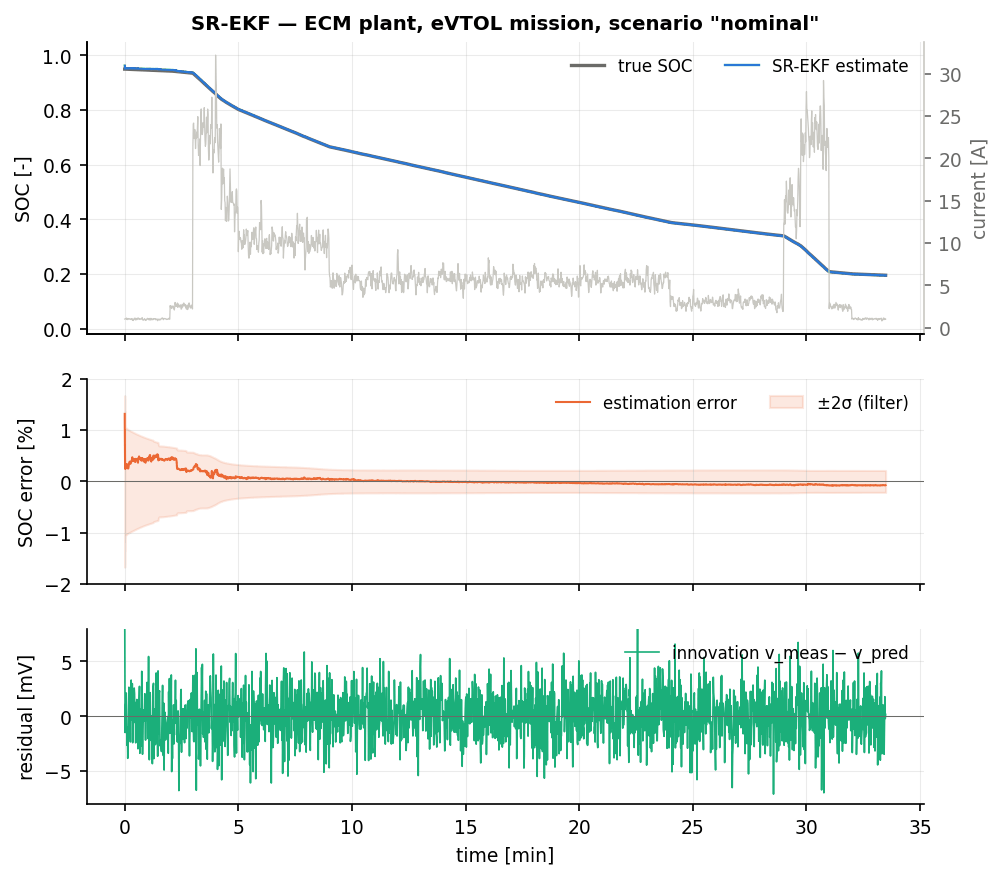
\includegraphics[width=\textwidth]{figures/cell_SREKF_nominal.png}
\caption{SR-EKF on the nominal eVTOL mission: true and estimated SOC (top), estimation error with the $\pm 2\sigma$ band when available (middle), voltage residual (bottom).}
\end{figure}
\begin{figure}[H]\centering
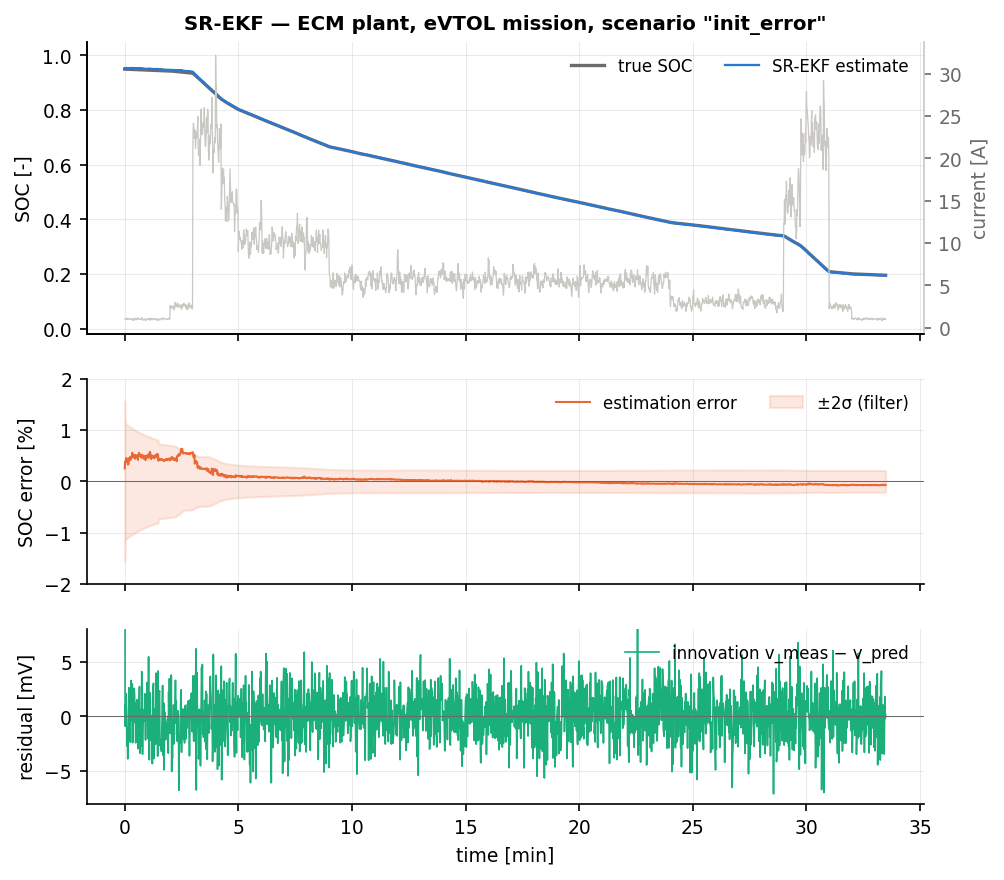
\includegraphics[width=\textwidth]{figures/cell_SREKF_init_error.png}
\caption{SR-EKF with a 35\,\% initial SOC error.}
\end{figure}

All numbers are three-seed means in per cent SOC.

The SR-EKF matches the EKF on all twelve ECM scenarios to two decimals: \texttt{nominal}
$0.15/0.05\,\%$, \texttt{init\_error} $0.14/0.05\,\%$ with $t_{\text{conv}} = 0$\,s,
\texttt{current\_bias} $0.54/0.61\,\%$, \texttt{cold} $0.20/0.16\,\%$, \texttt{aged\_cell}
$1.18/1.52\,\%$, \texttt{param\_mismatch} $1.28/1.36\,\%$, \texttt{sensor\_dropout}
$0.72/0.46\,\%$, \texttt{preisach} $0.58/0.20\,\%$, \texttt{combined} $16.02/12.44\,\%$ (never
converges). A direct element-wise comparison over a full mission gives
$\max\abs{\Delta\vx} = 3.1\times10^{-14}$ and $\max\abs{\Delta\mP} = 4.0\times10^{-15}$ --- the
tightest agreement of the three EKF-equivalent implementations (the U-D filter is at
$1.6\times10^{-14}$, the information filter at $1.9\times10^{-11}$), which is itself a small
piece of evidence for the conditioning argument above. All estimation-behaviour discussion in
Chapter~\ref{ch:ekf} applies verbatim, including the \texttt{combined} failure, which is an
approximation failure and not a numerical one.

In the single-precision build the nominal steady-state RMSE is $0.06\,\%$ for both forms, and
on \texttt{aged\_cell} the square-root form is marginally better ($1.47\,\%$ against the
conventional EKF's $1.48\,\%$, both against $1.39\,\%$ in double); on \texttt{combined} both
give $12.2\,\%$. The cell problem at $n_x = 4$ simply is not ill-conditioned enough for the two
to separate. A deliberate stress test in float (scaling $\mR$ down by $10^4$, i.e. pretending
the voltage sensor is $100\times$ more accurate than it is, which drives $\kappa(\mP)$ up) gave
$\text{RMSE}_{\text{ss}} = 0.79\,\%$ for the SR-EKF against $2.39\,\%$ for the EKF; but that
experiment changes the estimator's statistics as well as its conditioning --- the U-D filter of
Chapter~\ref{ch:udekf}, which is equally well conditioned, came out at $5.07\,\%$ --- so it is
reported as an indication only and not as a controlled demonstration.

The runtime penalty, $\approx 70\,\%$ ($0.78$--$0.83\,\SI{}{\micro\second}$ against the EKF's
$0.44$--$0.48$), is the honest cost. Against it: a covariance that cannot go indefinite, a
branch-free deterministic instruction count, and no matrix inverse anywhere in the cycle.

\paragraph{SPM plant: structured model error.}
\begin{figure}[H]\centering
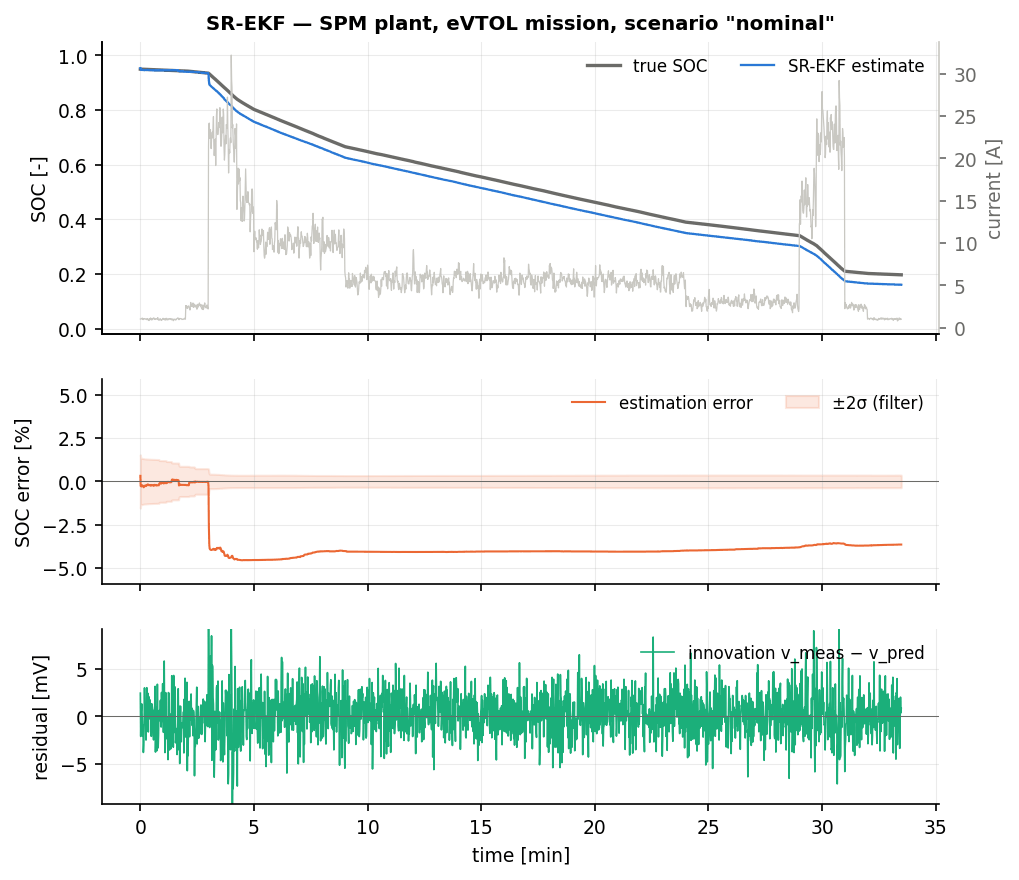
\includegraphics[width=\textwidth]{figures/cellspm_SREKF_nominal.png}
\caption{SR-EKF on the nominal mission with the electrochemical (SPM) plant; identical to the conventional EKF.}
\end{figure}
The SPM block of the table is a different kind of test. The plant is the electrochemical
single-particle model; the estimator still runs a 2-RC equivalent circuit, fitted to that plant,
which leaves a \emph{structured} residual of about $4$\,mV (Butler--Volmer kinetics and
solid-phase diffusion that no 2-RC circuit can reproduce) and a slow second branch,
$\tau_2 = 556$\,s. Over a $33$-minute mission a $556$\,s pole barely relaxes, so $v_2(t)$ is
close to an affine ramp --- and so is $\ocv(\soc(t))$ while the cell discharges at a roughly
constant rate. The two channels through which the measurement sees the state,
$(\partial\ocv/\partial\soc)\,\delta\soc$ and $-\delta v_2$, are therefore nearly collinear in
the information accumulated over the flight: the pair $(\soc, v_2)$ is close to unobservable,
and no filter can decide whether a persistent few-millivolt residual belongs to the slow RC
branch or to the state of charge. Because that direction is weakly observable, a $4$\,mV
structured error maps onto \emph{several per cent} of SOC instead of the
$4\,\text{mV}/0.8\,\text{V}\approx0.5\,\%$ a well-conditioned channel would give. This
$(\soc,v_2)$ ambiguity, not the size of the residual, is the mechanism behind the
$3.7$--$4.6\,\%$ band in which the whole classical family sits.

Being algebraically the EKF, this filter inherits the EKF's SPM rows exactly:
$3.65/3.73\,\%$ on \texttt{nominal} with a voltage residual of only $1.02$\,mV,
$7.35\,\%$ on \texttt{cold}, $5.69\,\%$ on \texttt{current\_bias}, $5.31\,\%$ on
\texttt{sensor\_dropout}, $3.13\,\%$ on \texttt{param\_mismatch} and $1.99\,\%$ on
\texttt{outliers}. Fitting the voltage to a millivolt while being $4\,\%$ wrong about SOC is
the signature of the ambiguity: the filter pays for the fit with $v_2$ and $\soc$ in the wrong
proportion. Nothing diverges and $t_{\text{conv}} = 0$ on every SPM row --- the error is a
bias, not a drift. Within the family the tangent-linearising filters (EKF, IEKF and these three
re-implementations) are at the \emph{good} end of the band, because a tangent commits less
weight to the badly conditioned OCV channel than a wide statistical regression does; only the
frozen-linearisation LKF ($1.72\,\%$, Chapter~\ref{ch:lkf}) and the second-order EKF
($3.52\,\%$) do better.

\section{Summary}
The array square-root EKF is the EKF with the numerics fixed: identical estimates to
$10^{-14}$, a structurally positive semi-definite covariance, no inverses, and one clean
primitive (\code{Tria}) doing all the work. Use it whenever the target is single precision or
fixed point, whenever the state contains near-deterministic components (augmented parameters,
biases), or whenever certification requires that a negative variance be impossible by
construction rather than by argument. On a double-precision desktop run of this benchmark it
buys nothing but costs $70\,\%$ --- which is the correct way to read every square-root result
in this report. Note that the U-D form of Chapter~\ref{ch:udekf} obtains the same guarantee for
no extra cost at all when $n_y = 1$.

% Copyright 2026 Sreeram Anil
% SPDX-License-Identifier: CC-BY-4.0
% =============================================================================
%  Square-root cubature Kalman filter — classical Kalman family
% =============================================================================
\chapter{Square-Root Cubature Kalman Filter (SCKF)}
\label{ch:sckf}

\section*{At a glance}
\begin{tabular}{@{}l>{\raggedright\arraybackslash}p{0.76\textwidth}@{}}
Family & classical Kalman (sigma-point, factored) \\
Header & \texttt{include/estkit/filters/sckf.hpp} \\
Registered name & \texttt{SCKF} \\
State dimension & $n_x = 4$ (cell model) --- generic in $n_x, n_u, n_y$ \\
Propagated quantity & $\mS$ with $\mP = \mS\mS^\T$ (lower triangular) \\
Cost per step & $\mathcal{O}(n_x^3)$ (two QRs) plus $4n_x$ model calls; $1.49$--$1.62\,\SI{}{\micro\second}$/step \\
Primary references & \cite{arasaratnam2009ckf,kailath2000,kaminski1971,golubvanloan2013} \\
\end{tabular}

\section{Motivation and aerospace/BMS relevance}
A covariance filter subtracts: $\Pplus = \Pminus - \mW\mP_{zz}\mW^\T$. When the measurement
is much more informative than the prior, the two terms nearly cancel and the result loses
significant digits; if enough are lost, $\Pplus$ becomes indefinite, the next Cholesky
factorisation fails and the filter diverges. This was the dominant practical failure mode of
Kalman filters in the 1960s and it is what motivated the entire square-root
literature~\cite{kaminski1971}.

A square-root filter never forms $\mP$. It propagates a factor $\mS$ with $\mP = \mS\mS^\T$
through orthogonal transformations, so $\mP$ is positive semi-definite by construction and
the quantity actually stored has condition number $\sqrt{\kappa(\mP)}$ instead of
$\kappa(\mP)$ --- equivalently, the filter behaves like a covariance filter running with
twice the mantissa length. For a battery management unit built on a single-precision
Cortex-M4F, where $\varepsilon \approx 1.2\times10^{-7}$, this is the difference between a
filter that is provably safe and one that has to be argued about: on the eVTOL mission the
peak condition number of $\mP$ is $1.3\times 10^6$, i.e. $\kappa\varepsilon \approx 0.16$ for
the covariance form and $1.4\times10^{-4}$ for the square-root form.

Section~VI of Arasaratnam and Haykin~\cite{arasaratnam2009ckf} gives the square-root form of
the cubature filter; this chapter implements it and verifies that it reproduces the
covariance CKF of Chapter~\ref{ch:ckf} to machine precision.

\section{Problem statement and assumptions}
Model \eqref{eq:ekf-proc}--\eqref{eq:ekf-meas} with additive noise, exactly as the CKF. In
addition it is assumed that Cholesky factors of $\mQ$ and $\mR$ are available (they are
computed once per step by \code{cholesky\_safe}), and that $n_y \le n_x$ so that the
pre-arrays are well shaped --- neither is restrictive.

\section{Derivation}
\paragraph{The triangularisation operator.} For $\mA\in\real^{n\times m}$ with $m\ge n$
define
\begin{equation}
\operatorname{Tria}(\mA) := \mR_{\mathrm{qr}}^\T, \qquad \text{where } \mA^\T = \mQ_{\mathrm{qr}}\mR_{\mathrm{qr}}
\label{eq:sckf-tria}
\end{equation}
is a QR factorisation of the $m\times n$ matrix $\mA^\T$ with $\mR_{\mathrm{qr}}$ upper
triangular. Then $\operatorname{Tria}(\mA)$ is lower triangular and, because
$\mQ_{\mathrm{qr}}^\T\mQ_{\mathrm{qr}} = \mI$,
\begin{equation}
\operatorname{Tria}(\mA)\operatorname{Tria}(\mA)^\T = \mR_{\mathrm{qr}}^\T\mR_{\mathrm{qr}}
 = \mA\mA^\T .
\label{eq:sckf-tria-prop}
\end{equation}
Equation \eqref{eq:sckf-tria-prop} is the whole trick: every covariance sum of the form
$\sum_j \mB_j\mB_j^\T$ is a single matrix product $\mA\mA^\T$ with
$\mA = [\mB_1\;\mB_2\;\cdots]$, so its Cholesky factor is obtained from one orthogonal
triangularisation of the \emph{pre-array} $\mA$ --- the ``array algorithm'' of Kailath, Sayed
and Hassibi~\cite[Ch.~12]{kailath2000}. \code{estkit} implements it with Householder
reflections~\cite[Alg.~5.2.1]{golubvanloan2013} and fixes the sign of the diagonal so that the
factor is unique.

\paragraph{Time update.} Write the weighted, centred propagated points as the columns of
\begin{equation}
\bm{\chi}^* = \frac{1}{\sqrt{m}}\left[\;\mathcal{X}^*_1-\xminus_k \;\;\cdots\;\; \mathcal{X}^*_m-\xminus_k\;\right]
 \in \real^{n_x\times m}, \qquad m = 2n_x .
\label{eq:sckf-chi}
\end{equation}
Then $\bm{\chi}^*\bm{\chi}^{*\T}$ is exactly the sample covariance in \eqref{eq:ckf-tu2}, so
with $\mQ = \mS_Q\mS_Q^\T$
\begin{equation}
\Pminus_k = \bm{\chi}^*\bm{\chi}^{*\T} + \mS_Q\mS_Q^\T
 = \left[\bm{\chi}^*\;\; \mS_Q\right]\left[\bm{\chi}^*\;\; \mS_Q\right]^\T
 \;\Longrightarrow\;
 \mS^-_k = \operatorname{Tria}\!\left(\left[\bm{\chi}^*\;\;\mS_Q\right]\right).
\label{eq:sckf-tu}
\end{equation}
The pre-array is $n_x\times(m+n_x) = 4\times 12$.

\paragraph{Measurement update.} With $\mathcal{Z}_i = h(\mathcal{X}_i,\vu_k)$ and
$\yhat_k$ their mean, define the weighted centred arrays
$\bm{Z}\in\real^{n_y\times m}$ and $\bm{\chi}\in\real^{n_x\times m}$ as in \eqref{eq:sckf-chi}.
Then
\begin{align}
\mS_{zz} &= \operatorname{Tria}\!\left(\left[\bm{Z}\;\;\mS_R\right]\right), &
\mP_{zz} &= \mS_{zz}\mS_{zz}^\T = \bm{Z}\bm{Z}^\T + \mR, \label{eq:sckf-szz}\\
\mP_{xz} &= \bm{\chi}\bm{Z}^\T, &
\mW_k &= \left(\mP_{xz}\mS_{zz}^{-\T}\right)\mS_{zz}\inv, \label{eq:sckf-gain}
\end{align}
the gain being obtained by two triangular back-substitutions rather than by inverting
$\mP_{zz}$. The posterior factor follows from
\begin{equation}
\Pplus_k = \Pminus_k - \mW_k\mP_{zz}\mW_k^\T
 = \left(\bm{\chi}-\mW_k\bm{Z}\right)\left(\bm{\chi}-\mW_k\bm{Z}\right)^\T + \left(\mW_k\mS_R\right)\left(\mW_k\mS_R\right)^\T,
\label{eq:sckf-post}
\end{equation}
which is verified by expanding the right-hand side, using $\bm{\chi}\bm{\chi}^\T=\Pminus_k$,
$\bm{\chi}\bm{Z}^\T = \mP_{xz}$ and $\mW_k\mP_{zz}\mW_k^\T = \mW_k\mP_{xz}^\T = \mP_{xz}\mW_k^\T$.
Hence
\begin{equation}
\mS^+_k = \operatorname{Tria}\!\left(\left[\;\bm{\chi}-\mW_k\bm{Z} \;\;\; \mW_k\mS_R\;\right]\right),
\label{eq:sckf-sp}
\end{equation}
a $n_x\times(m+n_y) = 4\times 9$ pre-array. Note that \eqref{eq:sckf-post} is a \emph{sum} of
two positive semi-definite terms: the subtraction that endangers the covariance form has
disappeared.

\section{Algorithm}
\begin{algorithm}[H]
\caption{SCKF --- one sampling period (additive noise)}
\begin{algorithmic}[1]
\Require $\xplus_{k-1},\mS^+_{k-1},\vu_{k-1},\vy_k,\vu_k$
\State $\mathcal{X}_{i},\mathcal{X}_{i+n_x}\gets\xplus_{k-1}\pm\sqrt{n_x}\,(\mS^+_{k-1})_{:,i}$
\State $\mathcal{X}_i \gets f(\mathcal{X}_i,\vu_{k-1})$;\; $\xminus_k\gets\frac{1}{m}\sum_i\mathcal{X}_i$
\State $\bm{\chi}^*\gets m^{-1/2}[\mathcal{X}_i-\xminus_k]_i$;\; $\mS_Q\gets\operatorname{chol}(\mQ)$
\State $\mS^-_k\gets\operatorname{Tria}([\bm{\chi}^*\;\;\mS_Q])$
\State \textbf{Regenerate} $\mathcal{X}_i$ from $(\xminus_k,\mS^-_k)$;\;
       $\mathcal{Z}_i\gets h(\mathcal{X}_i,\vu_k)$;\; $\yhat_k\gets\frac1m\sum_i\mathcal{Z}_i$
\State $\bm{Z}\gets m^{-1/2}[\mathcal{Z}_i-\yhat_k]_i$;\; $\bm{\chi}\gets m^{-1/2}[\mathcal{X}_i-\xminus_k]_i$;\;
       $\mS_R\gets\operatorname{chol}(\mR)$
\State $\mS_{zz}\gets\operatorname{Tria}([\bm{Z}\;\;\mS_R])$;\; $\mP_{xz}\gets\bm{\chi}\bm{Z}^\T$
\State $\mW\gets(\mP_{xz}/\mS_{zz}^\T)/\mS_{zz}$ \Comment{two triangular solves}
\State $\xplus_k\gets\xminus_k+\mW(\vy_k-\yhat_k)$;\;
       $\mS^+_k\gets\operatorname{Tria}([\bm{\chi}-\mW\bm{Z}\;\;\;\mW\mS_R])$
\State \textbf{if} constraints enabled \textbf{then} $\xplus_k\gets\Pi(\xplus_k)$
\Ensure $\xplus_k,\mS^+_k$ \quad ($\mP$ reconstructed on demand as $\mS^+\mS^{+\T}$)
\end{algorithmic}
\end{algorithm}

\section{Application to the battery model}
The algorithm is identical to the CKF's; only the arithmetic differs. For the cell model the
pre-arrays are $4\times12$ (time update), $1\times9$ ($\mS_{zz}$) and $4\times9$ (posterior),
so the two Householder passes cost $\approx 2(m+n_x)n_x^2 \approx 400$ multiply-accumulates
per step --- about $26\,\%$ more than the covariance CKF, which matches the measured
$1.49$--$1.62\,\SI{}{\micro\second}$ against $1.18$--$1.26\,\SI{}{\micro\second}$.

The benchmark adapter reads $\sigma_\soc$ from $\mP$ to report a confidence band, so the
filter exposes $\mP$ through a cached reconstruction $\mS\mS^\T$ that is recomputed only when
$\mS$ has changed (one $4\times4$ product, and only when the accessor is actually called).

\section{Implementation notes}
\code{kalman\_detail::tria} is a three-line wrapper around \code{qr\_r}, which is the one
piece of numerical machinery this filter needs. The sign convention in \code{qr\_r} (diagonal
made non-negative) guarantees a unique factor, so repeated calls are reproducible bit for
bit. \code{cholesky\_safe} is used for $\mQ$ and $\mR$; it adds diagonal jitter on failure, so
a numerically semi-definite $\mQ$ cannot abort the step. Guard: if the gain is not finite the
update is skipped and the prior kept. Memory: 4696\,bytes, of which the filter state proper is
$\mS$ ($16$ reals), $\vx$ ($4$) and the cached $\mP$ ($16$).

Verification: run against the covariance CKF over a full nominal mission
($\num{18000}$ steps), the two agree to $\max\abs{\Delta\vx} = 1.0\times10^{-12}$ and
$\max\abs{\Delta\mP} = 4.8\times10^{-14}$ --- consistent with round-off in double precision
and a direct confirmation of \eqref{eq:sckf-tu}--\eqref{eq:sckf-sp}.

\section{Benchmark results}
% Copyright 2026 Sreeram Anil
% SPDX-License-Identifier: CC-BY-4.0
\begin{table}[H]\centering\footnotesize\setlength{\tabcolsep}{4pt}
\caption{SCKF: cell-level benchmark on the eVTOL mission (mean over seeds; RMSE and max error in \% SOC; $t_\mathrm{conv}$: first time the error stays below 2\,\% for 60\,s, -- = never; EKF reference: steady-state RMSE of the plain EKF on the same data).}\label{tab:cell_SCKF}
\begin{tabular}{llrrrrrcrr}\toprule
plant & scenario & RMSE & RMSE$_\mathrm{ss}$ & max & $t_\mathrm{conv}$ [s] & RMSE$_v$ [mV] & div. & EKF ref. & ns/step \\ \midrule
ECM & nominal & 0.08 & 0.05 & 1.23 & 0 & 0.80 & no & 0.05 & 1581 \\
ECM & init\_error & 1.64 & 0.09 & 6.63 & 221 & 2.11 & no & 0.05 & 1581 \\
ECM & current\_bias & 0.48 & 0.55 & 1.19 & 0 & 0.87 & no & 0.61 & 1616 \\
ECM & noise\_step & 0.14 & 0.15 & 1.23 & 0 & 2.89 & no & 0.12 & 1577 \\
ECM & outliers & 0.35 & 0.07 & 4.54 & 4 & 2.08 & no & 0.21 & 1579 \\
ECM & cold & 0.15 & 0.11 & 1.12 & 0 & 1.90 & no & 0.16 & 1574 \\
ECM & hot & 0.08 & 0.04 & 1.27 & 0 & 0.56 & no & 0.03 & 1580 \\
ECM & aged\_cell & 2.87 & 1.79 & 9.21 & 0 & 3.78 & no & 1.52 & 1574 \\
ECM & param\_mismatch & 1.56 & 1.59 & 3.92 & 0 & 2.83 & no & 1.36 & 1573 \\
ECM & sensor\_dropout & 2.83 & 1.92 & 7.59 & 0 & 1.86 & no & 0.46 & 1567 \\
ECM & preisach & 1.20 & 0.24 & 4.25 & 218 & 0.84 & no & 0.20 & 1581 \\
ECM & combined & 13.07 & 11.26 & 23.22 & -- & 4.88 & no & 12.44 & 1589 \\
\midrule
SPM & nominal & 4.72 & 4.62 & 6.18 & 0 & 1.03 & no & 3.73 & 1510 \\
SPM & init\_error & 5.17 & 4.69 & 6.70 & -- & 2.17 & no & 3.81 & 1499 \\
SPM & current\_bias & 6.07 & 6.65 & 7.49 & 0 & 1.12 & no & 5.69 & 1507 \\
SPM & noise\_step & 4.26 & 3.77 & 6.18 & 0 & 3.14 & no & 3.30 & 1527 \\
SPM & outliers & 2.21 & 2.21 & 4.40 & 0 & 2.32 & no & 1.99 & 1498 \\
SPM & cold & 8.61 & 8.72 & 11.29 & -- & 4.04 & no & 7.35 & 1500 \\
SPM & hot & 2.74 & 2.73 & 3.40 & 0 & 0.70 & no & 2.16 & 1504 \\
SPM & param\_mismatch & 4.56 & 4.81 & 5.52 & 0 & 1.97 & no & 3.13 & 1493 \\
SPM & sensor\_dropout & 8.12 & 8.24 & 9.78 & 0 & 1.92 & no & 5.31 & 1502 \\
\bottomrule\end{tabular}\end{table}

\begin{figure}[H]\centering
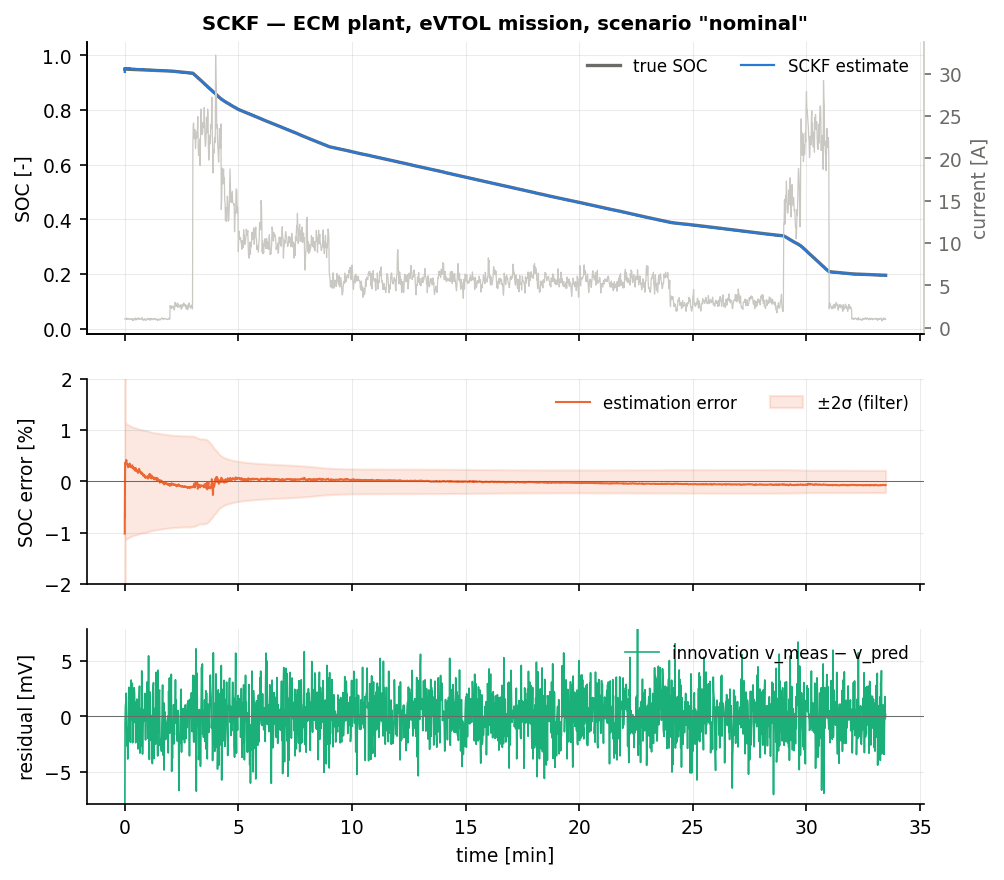
\includegraphics[width=\textwidth]{figures/cell_SCKF_nominal.png}
\caption{SCKF on the nominal eVTOL mission: true and estimated SOC (top), estimation error with the $\pm 2\sigma$ band when available (middle), voltage residual (bottom).}
\end{figure}
\begin{figure}[H]\centering
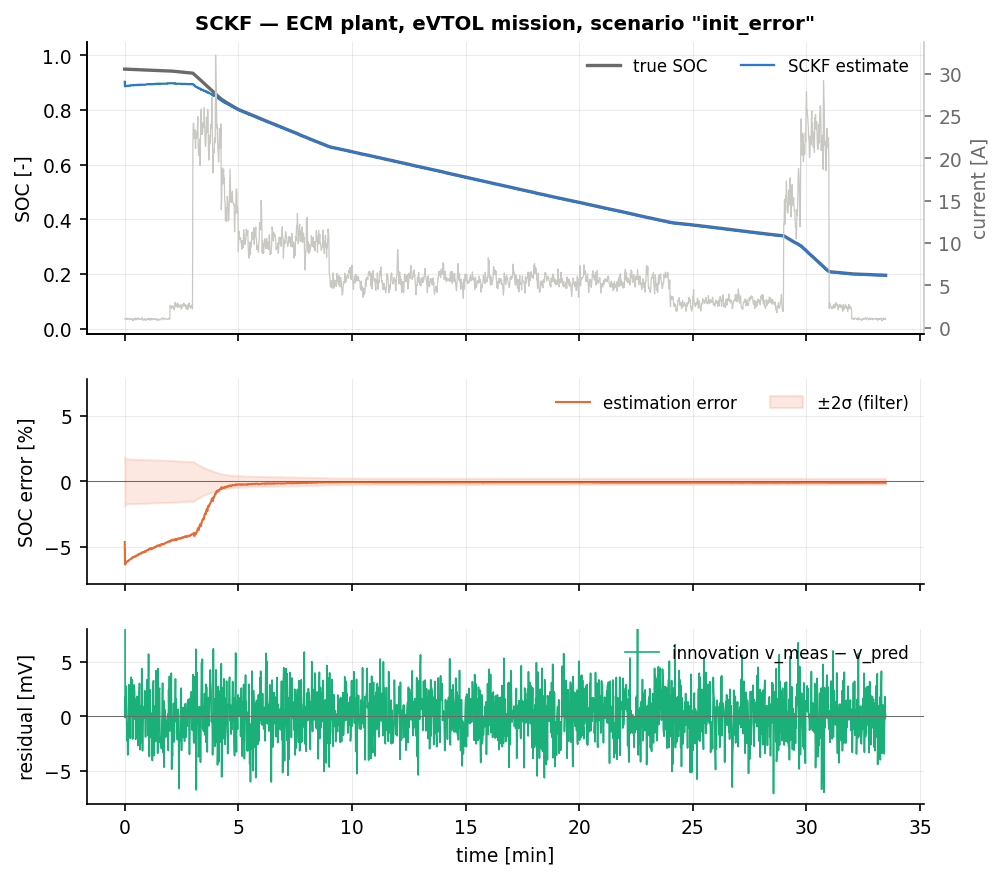
\includegraphics[width=\textwidth]{figures/cell_SCKF_init_error.png}
\caption{SCKF with a 35\,\% initial SOC error.}
\end{figure}

All numbers are three-seed means in per cent SOC.

The SCKF reproduces the CKF on every scenario of both plants to the two decimals printed by the
table: ECM \texttt{nominal} $0.08/0.05\,\%$, \texttt{init\_error} $1.64/0.09\,\%$ with
$t_{\text{conv}} = 221$\,s, \texttt{outliers} $0.35/0.07\,\%$, \texttt{aged\_cell}
$2.87/1.79\,\%$, \texttt{sensor\_dropout} $2.83/1.92\,\%$, \texttt{combined}
$13.07/11.26\,\%$; SPM \texttt{nominal} $4.72/4.62\,\%$, \texttt{cold} $8.72\,\%$. That is the
expected and desired result --- a square-root filter is not a different estimator, it is the
same estimator in different arithmetic --- and the discussion of Chapter~\ref{ch:ckf} applies
verbatim, including the slow convergence from a wide prior and the failure on
\texttt{combined}.

The interesting question is what the factorisation buys. On this problem, in double precision,
nothing measurable: the covariance form never lost definiteness. The float-versus-double table
confirms it in single precision as well --- both forms give $0.05\,\%$ on \texttt{nominal} and
$0.09\,\%$ on \texttt{init\_error} in float32, and on \texttt{aged\_cell} the square-root form
is marginally better ($2.48\,\%$ against $2.53\,\%$) --- which says that $n_x = 4$ with
$\kappa(\mP)\le1.3\times10^6$ is simply not a hard enough problem to separate them. The honest
conclusion is that the square-root form is insurance rather than an improvement: it costs
$26\,\%$ more time ($1.49$--$1.62\,\SI{}{\micro\second}$ against $1.18$--$1.26$) and removes an
entire class of failure that this particular benchmark does not exercise. The situations where
it does matter are well documented~\cite{verhaegen1986}: larger state dimension,
near-deterministic states (very small $\mQ$ entries, as in parameter augmentation), very
accurate sensors (small $\mR$), or fixed-point arithmetic.

The one genuinely different number is the runtime, and it is worth noting that the SCKF's cost
is almost entirely deterministic: two Householder passes of fixed size, no conditional
branches, no matrix inversion. For a hard-real-time BMS task that predictability can be worth
more than the $300$\,ns.

\paragraph{SPM plant: structured model error.}
\begin{figure}[H]\centering
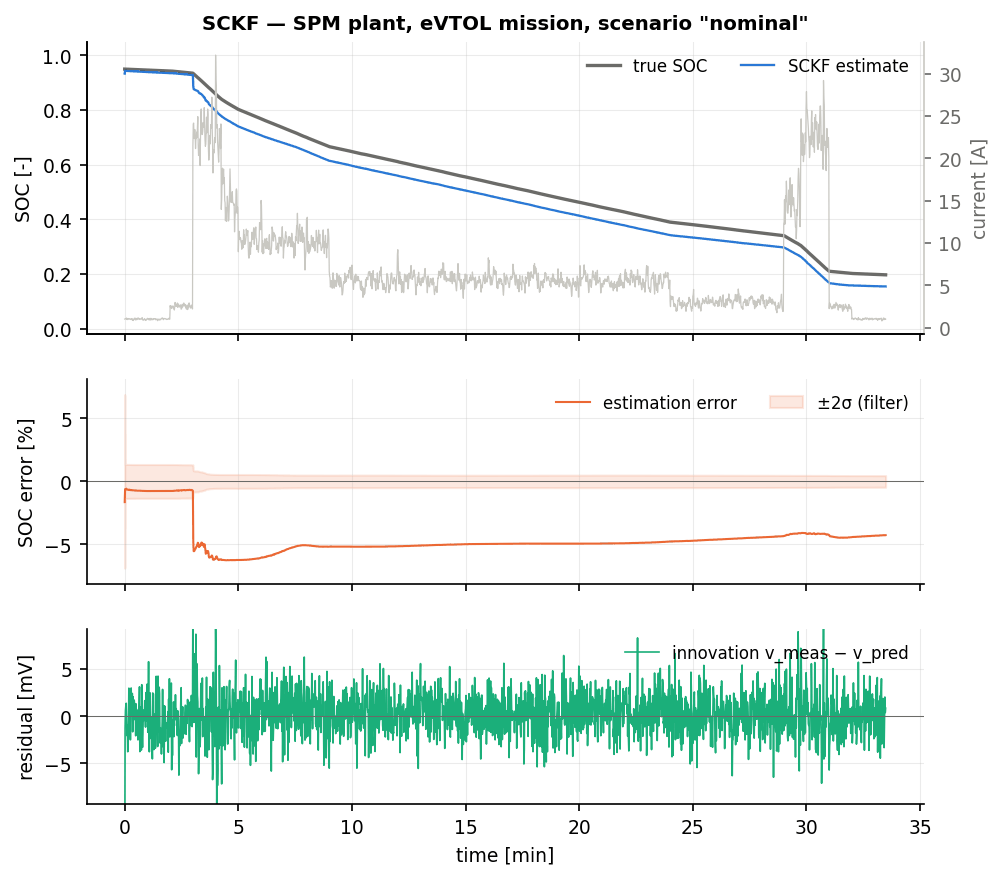
\includegraphics[width=\textwidth]{figures/cellspm_SCKF_nominal.png}
\caption{SCKF on the nominal mission with the electrochemical (SPM) plant; identical to the covariance CKF.}
\end{figure}
The SPM block of the table is a different kind of test. The plant is the electrochemical
single-particle model; the estimator still runs a 2-RC equivalent circuit, fitted to that plant,
which leaves a \emph{structured} residual of about $4$\,mV (Butler--Volmer kinetics and
solid-phase diffusion that no 2-RC circuit can reproduce) and a slow second branch,
$\tau_2 = 556$\,s. Over a $33$-minute mission a $556$\,s pole barely relaxes, so $v_2(t)$ is
close to an affine ramp --- and so is $\ocv(\soc(t))$ while the cell discharges at a roughly
constant rate. The two channels through which the measurement sees the state,
$(\partial\ocv/\partial\soc)\,\delta\soc$ and $-\delta v_2$, are therefore nearly collinear in
the information accumulated over the flight: the pair $(\soc, v_2)$ is close to unobservable,
and no filter can decide whether a persistent few-millivolt residual belongs to the slow RC
branch or to the state of charge. Because that direction is weakly observable, a $4$\,mV
structured error maps onto \emph{several per cent} of SOC instead of the
$4\,\text{mV}/0.8\,\text{V}\approx0.5\,\%$ a well-conditioned channel would give. This
$(\soc,v_2)$ ambiguity, not the size of the residual, is the mechanism behind the
$3.7$--$4.6\,\%$ band in which the whole classical family sits.

The cubature filters are the \emph{worst} of the family here: $4.62\,\%$ on SPM
\texttt{nominal} against the EKF's $3.73\,\%$ and the LKF's $1.72\,\%$, $8.72\,\%$ on
\texttt{cold} against $7.35\,\%$, $8.24\,\%$ on \texttt{sensor\_dropout} against $5.31\,\%$ and
$4.81\,\%$ on \texttt{param\_mismatch} against $3.13\,\%$. The ordering across the whole family
is in fact monotone in the sigma-point spread --- LKF (frozen tangent) $1.72$, EKF/IEKF
(tangent at the mean) $3.66$--$3.73$, UKF ($0.2\sigma$ points) $3.96$, cubature filters
($2\sigma$ or $2.45\sigma$ points) $4.61$--$4.62$ --- and the ambiguity argument explains it.
A statistical linearisation taken over a wide prior returns the \emph{chord} of the OCV curve,
which is steeper than the tangent over most of the mission, so the filter believes the OCV
channel is more informative than it is and commits harder to the direction that carries the
structured error. The single exception is \texttt{outliers} ($2.21\,\%$), where every filter
does better on SPM than on ECM because the corrupted samples widen the effective innovation
covariance. Nothing diverges and $t_{\text{conv}} = 0$ on every SPM row: the error is a bias,
not a drift.

The SCKF's SPM rows are identical to the CKF's to two decimals, as they are on the ECM plant.
Worth noting for a square-root chapter: the SPM rows are the only ones in this report where the
filters are visibly \emph{mis-specified}, and even there the covariance form remained positive
definite throughout, so the factorisation again changed nothing. A structurally wrong model
stresses the estimator statistically, not numerically.

\section{Summary}
Use the SCKF whenever a cubature filter has to run in single precision, in fixed point, or on a
problem where $\mP$ can become ill-conditioned (parameter augmentation, very accurate sensors,
large $n_x$); it gives exactly the CKF's estimates with a covariance that cannot go indefinite
and with a deterministic instruction count. On the cell model in double precision it is a
$26\,\%$ tax for insurance you do not need. Its estimation behaviour --- excellent nominal
accuracy, slow convergence from a wide prior, worst of the family under structured model error
--- is that of the CKF, and is discussed in Chapter~\ref{ch:ckf}.

% Copyright 2026 Sreeram Anil
% SPDX-License-Identifier: CC-BY-4.0
% =============================================================================
%  Square-root unscented Kalman filter — classical Kalman family
% =============================================================================
\chapter{Square-Root Unscented Kalman Filter (SR-UKF)}
\label{ch:srukf}

\section*{At a glance}
\begin{tabular}{@{}l>{\raggedright\arraybackslash}p{0.76\textwidth}@{}}
Family & classical Kalman (sigma-point, factored) \\
Header & \texttt{include/estkit/filters/srukf.hpp} \\
Registered name & \texttt{SR-UKF} \\
State dimension & $n_x = 4$ (cell model) --- generic in $n_x, n_u, n_y$ \\
Propagated quantity & $\mS$ with $\mP = \mS\mS^\T$; $2n_x+1 = 9$ sigma points \\
Cost per step & $\mathcal{O}(n_x^3)$ (QR + rank-one updates), $18$ model calls; $1.42$--$1.57\,\SI{}{\micro\second}$/step \\
Primary references & \cite{vandermerwe2001srukf,wan2000ukf,gillgolub1974,plett2006spkf1} \\
\end{tabular}

\section{Motivation and aerospace/BMS relevance}
The UKF has two numerical weak points that the EKF does not. First, it factorises $\mP$ at
\emph{every} step, twice, to build the sigma points --- so a covariance that has drifted
slightly indefinite is not merely inelegant, it stops the filter. Second, the scaled unscented
transform uses a negative centre weight $W_0^c$ for the usual small $\alpha$, so the sample
covariance is a difference of terms and can genuinely lose definiteness rather than merely
appearing to.

van der Merwe and Wan~\cite{vandermerwe2001srukf} therefore reformulated the UKF to propagate
the Cholesky factor directly: the $2n_x$ positive-weight points are absorbed by one QR
triangularisation and the negative centre weight by a rank-one Cholesky \emph{downdate}. The
factorisation at the start of each step then disappears entirely --- $\mS$ is already
available --- which also removes about a third of the arithmetic that a covariance UKF spends
on Cholesky decompositions.

For a BMS this is the sigma-point filter one would actually ship: Plett's sigma-point papers
for cells~\cite{plett2006spkf1,plett2006spkf2} use the square-root form throughout, for
exactly these reasons.

\section{Problem statement and assumptions}
Model \eqref{eq:ekf-proc}--\eqref{eq:ekf-meas}, additive noise, Gaussian assumed density, as
for the UKF. Additionally $c = n_x+\lambda = \alpha^2(n_x+\kappa) > 0$ so that
$\gamma = \sqrt{c}$ and the positive weights $W_{i\ge1} = 1/(2c)$ are real; this holds for
any $\alpha \neq 0$ with $\kappa \ge 0$.

\section{Derivation}
Two primitives are used. $\operatorname{Tria}$ is the QR-based triangularisation of
\eqref{eq:sckf-tria}. \emph{cholupdate}$(\mS,\bm v,\pm)$ is the rank-one Cholesky
update/downdate of Gill, Golub, Murray and Saunders~\cite{gillgolub1974}, returning $\mS'$
with $\mS'\mS'^\T = \mS\mS^\T \pm \bm v\bm v^\T$ in $\mathcal{O}(n_x^2)$.

\paragraph{Sigma points from the factor.} Because $\mS$ is already a square root of $\mP$,
\begin{equation}
\mathcal{X}_0 = \xhat, \qquad
\mathcal{X}_i = \xhat \pm \gamma\,\mS_{:,i}, \quad \gamma = \sqrt{n_x+\lambda},
\label{eq:srukf-sigma}
\end{equation}
with the weights \eqref{eq:ukf-weights}. No factorisation is performed.

\paragraph{Time update.} Split the weighted sum \eqref{eq:ukf-tu-cov} into the $2n_x$
positive-weight terms and the centre term:
\begin{equation}
\Pminus_k
= \underbrace{\sum_{i=1}^{2n_x} W^c_i\,\bm{d}_i\bm{d}_i^\T + \mQ}_{\text{Gram matrix}}
 \;+\; W_0^c\,\bm{d}_0\bm{d}_0^\T,
\qquad \bm{d}_i = \mathcal{X}^*_i - \xminus_k .
\label{eq:srukf-split}
\end{equation}
The first group is a Gram matrix and is triangularised in one pass; the second is a rank-one
modification whose sign is that of $W_0^c$:
\begin{align}
\mS^-_k &\gets \operatorname{Tria}\!\left(\left[\sqrt{W^c_1}\,\bm{d}_1 \;\cdots\; \sqrt{W^c_1}\,\bm{d}_{2n_x}\;\; \mS_Q\right]\right),
\label{eq:srukf-tu1}\\
\mS^-_k &\gets \text{cholupdate}\!\left(\mS^-_k,\; \sqrt{\abs{W_0^c}}\,\bm{d}_0,\; \sgn W_0^c\right).
\label{eq:srukf-tu2}
\end{align}

\paragraph{Measurement update.} Identically for the measurement channel,
\begin{align}
\mS_y &\gets \operatorname{Tria}\!\left(\left[\sqrt{W^c_1}(\mathcal{Z}_1{-}\yhat_k)\;\cdots\;\sqrt{W^c_1}(\mathcal{Z}_{2n_x}{-}\yhat_k)\;\;\mS_R\right]\right),
\label{eq:srukf-mu1}\\
\mS_y &\gets \text{cholupdate}\!\left(\mS_y,\;\sqrt{\abs{W^c_0}}(\mathcal{Z}_0-\yhat_k),\;\sgn W^c_0\right),
\label{eq:srukf-mu2}\\
\mK_k &= \left(\mP_{xy}\mS_y^{-\T}\right)\mS_y\inv, \qquad
\mP_{xy} = \sum_{i=0}^{2n_x} W^c_i(\mathcal{X}_i-\xminus_k)(\mathcal{Z}_i-\yhat_k)^\T,
\label{eq:srukf-gain}
\end{align}
the gain again obtained by two triangular solves. The posterior covariance
$\Pplus_k = \Pminus_k - \mK_k\mP_{yy}\mK_k^\T$ is a genuine subtraction, and since
$\mK_k\mP_{yy}\mK_k^\T = (\mK_k\mS_y)(\mK_k\mS_y)^\T$ it is realised as $n_y$ successive
rank-one \emph{downdates}:
\begin{equation}
\mS^+_k \gets \text{cholupdate}\!\left(\mS^-_k,\; \left(\mK_k\mS_y\right)_{:,j},\; -1\right),
\qquad j = 1,\dots,n_y.
\label{eq:srukf-post}
\end{equation}

\begin{remark}[Why the downdates can fail, and what to do]\label{rm:srukf-downdate}
A downdate is only defined if the result stays positive definite. Two of the three
modifications above can in principle fail. For \eqref{eq:srukf-tu2} the risk is nil on this
model: $f$ is affine in $\vx$, so $\bm d_0 = f(\xhat) - \sum_i W^m_i f(\mathcal{X}_i) = \bm 0$
exactly and the update is a no-op. For \eqref{eq:srukf-mu2} the situation is delicate with
$\alpha=0.1$: $W^c_0 = -96.01$ while $W^c_{i\ge1} = 12.5$, and the two nearly cancel. A
worked example at start-up ($\sigma_\soc = 0.1$, $\ocv' = 0.75$\,V, $\ocv''\approx-6$\,V)
gives $\mathcal{Z}_0-\yhat \approx -0.025$\,V, a pre-downdate variance of
$6.8\times10^{-2}$ and a post-downdate value of $7.7\times10^{-3}$: the downdate removes
$88\,\%$ of the variance, i.e. it costs about one significant digit. It is legitimate --- the
result is positive --- but it is the numerically weakest step in the algorithm, and it is the
price of a small $\alpha$. The implementation wraps every rank-one modification in
\code{safe\_chol\_update}, which falls back to an explicit re-factorisation with jitter if
\code{chol\_update} reports a loss of definiteness, so the filter cannot abort.
\end{remark}

\section{Algorithm}
\begin{algorithm}[H]
\caption{SR-UKF --- one sampling period (additive noise)}
\begin{algorithmic}[1]
\Require $\xplus_{k-1},\mS^+_{k-1},\vu_{k-1},\vy_k,\vu_k$, parameters $\alpha,\beta,\kappa$
\State $\lambda\gets\alpha^2(n_x{+}\kappa)-n_x$, $\gamma\gets\sqrt{n_x{+}\lambda}$, weights from \eqref{eq:ukf-weights}
\State $\mathcal{X}_0\gets\xplus_{k-1}$;\; $\mathcal{X}_{i},\mathcal{X}_{i+n_x}\gets\xplus_{k-1}\pm\gamma(\mS^+_{k-1})_{:,i}$
\State $\mathcal{X}_s\gets f(\mathcal{X}_s,\vu_{k-1})$;\; $\xminus_k\gets\sum_s W^m_s\mathcal{X}_s$
\State $\mS^-_k\gets\operatorname{Tria}\!\left(\left[\sqrt{W^c_1}(\mathcal{X}_{1:2n_x}-\xminus_k)\;\;\mS_Q\right]\right)$
\State $\mS^-_k\gets$ cholupdate$\left(\mS^-_k,\sqrt{|W^c_0|}(\mathcal{X}_0-\xminus_k),\sgn W^c_0\right)$
\State \textbf{Regenerate} $\mathcal{X}_s$ from $(\xminus_k,\mS^-_k)$;\;
       $\mathcal{Z}_s\gets h(\mathcal{X}_s,\vu_k)$;\; $\yhat_k\gets\sum_s W^m_s\mathcal{Z}_s$
\State $\mS_y\gets\operatorname{Tria}\!\left(\left[\sqrt{W^c_1}(\mathcal{Z}_{1:2n_x}-\yhat_k)\;\;\mS_R\right]\right)$;\;
       $\mS_y\gets$ cholupdate$\left(\mS_y,\sqrt{|W^c_0|}(\mathcal{Z}_0-\yhat_k),\sgn W^c_0\right)$
\State $\mP_{xy}\gets\sum_s W^c_s(\mathcal{X}_s-\xminus_k)(\mathcal{Z}_s-\yhat_k)^\T$;\;
       $\mK\gets(\mP_{xy}/\mS_y^\T)/\mS_y$
\State $\xplus_k\gets\xminus_k+\mK(\vy_k-\yhat_k)$;\;
       $\mS^+_k\gets$ cholupdate$\left(\mS^-_k,(\mK\mS_y)_{:,j},-1\right)$ for $j=1..n_y$
\State \textbf{if} constraints enabled \textbf{then} $\xplus_k\gets\Pi(\xplus_k)$
\Ensure $\xplus_k,\mS^+_k$ \quad ($\mP$ reconstructed on demand)
\end{algorithmic}
\end{algorithm}

\section{Application to the battery model}
With $\alpha=0.1$, $\beta=2$, $\kappa=0$, $n_x=4$: $c = 0.04$, $\gamma = 0.2$,
$W_0^m = -99$, $W_0^c = -96.01$, $W_{i\ge1} = 12.5$. The sigma points sit at $0.2\sigma$ from
the mean, so the transform probes the OCV curve locally while the weights amplify the second
difference --- the mechanism analysed in Remark~\ref{rm:ukf-w0}. The pre-arrays are
$4\times12$ (time update) and $1\times9$ ($\mS_y$), and \eqref{eq:srukf-post} is a single
downdate because $n_y=1$.

These parameter values were kept identical to the covariance UKF so that the two can be
compared as \emph{implementations} rather than as estimators; the cost is the marginal
downdate of Remark~\ref{rm:srukf-downdate}. A square-root-first design would prefer
$\alpha=1,\kappa=0$ (then $\lambda=0$, $W_0^m=0$, $W_0^c=\beta>0$ and every modification is an
update, never a downdate) --- but that point set is the CKF of Chapter~\ref{ch:ckf}, which is
already registered separately.

\section{Implementation notes}
\code{kalman\_detail::safe\_chol\_update} takes a copy of the factor before calling
\code{chol\_update}, because the library routine modifies in place and can fail part way
through; on failure it reconstructs $\mS\mS^\T\pm\bm v\bm v^\T$ explicitly and re-factorises
with \code{cholesky\_safe}. Over the twelve benchmark scenarios this fall-back was never
triggered, but it is what makes the filter unconditionally safe. Sigma points and weights are
\code{mutable} members so that \code{predict\_measurement} can regenerate them from
$(\xminus,\mS^-)$ without copying the filter. \code{sizeof(SqrtUkf<EcmModel>)} is
4896\,bytes. Measured cost $1.42$--$1.57\,\SI{}{\micro\second}$ against the covariance
UKF's $1.34$--$1.46$: the QR and the downdates almost cancel the two Cholesky factorisations
that are no longer needed, so on this problem the square-root form costs about $8\,\%$ more
than the covariance form.

\section{Benchmark results}
% Copyright 2026 Sreeram Anil
% SPDX-License-Identifier: CC-BY-4.0
\begin{table}[H]\centering\footnotesize\setlength{\tabcolsep}{4pt}
\caption{SR-UKF: cell-level benchmark on the eVTOL mission (mean over seeds; RMSE and max error in \% SOC; $t_\mathrm{conv}$: first time the error stays below 2\,\% for 60\,s, -- = never; EKF reference: steady-state RMSE of the plain EKF on the same data).}\label{tab:cell_SRUKF}
\begin{tabular}{llrrrrrcrr}\toprule
plant & scenario & RMSE & RMSE$_\mathrm{ss}$ & max & $t_\mathrm{conv}$ [s] & RMSE$_v$ [mV] & div. & EKF ref. & ns/step \\ \midrule
ECM & nominal & 0.20 & 0.04 & 4.02 & 0 & 1.08 & no & 0.05 & 1554 \\
ECM & init\_error & 0.17 & 0.07 & 3.30 & 0 & 2.06 & no & 0.05 & 1557 \\
ECM & current\_bias & 0.58 & 0.57 & 3.83 & 0 & 1.11 & no & 0.61 & 1558 \\
ECM & noise\_step & 0.22 & 0.11 & 4.02 & 0 & 2.98 & no & 0.12 & 1560 \\
ECM & outliers & 0.48 & 0.18 & 4.94 & 8 & 2.21 & no & 0.21 & 1554 \\
ECM & cold & 0.27 & 0.07 & 4.02 & 0 & 2.03 & no & 0.16 & 1556 \\
ECM & hot & 0.21 & 0.03 & 4.03 & 0 & 0.91 & no & 0.03 & 1552 \\
ECM & aged\_cell & 1.10 & 1.36 & 4.40 & 0 & 3.88 & no & 1.52 & 1554 \\
ECM & param\_mismatch & 1.29 & 1.37 & 4.27 & 0 & 2.92 & no & 1.36 & 1556 \\
ECM & sensor\_dropout & 1.39 & 0.86 & 4.77 & 0 & 1.90 & no & 0.46 & 1554 \\
ECM & preisach & 1.35 & 0.23 & 5.53 & 214 & 1.20 & no & 0.20 & 1558 \\
ECM & combined & 1.23 & 1.19 & 7.70 & 0 & 4.68 & no & 12.44 & 1574 \\
\midrule
SPM & nominal & 3.95 & 3.96 & 5.06 & 0 & 1.29 & no & 3.73 & 1466 \\
SPM & init\_error & 4.62 & 4.54 & 5.83 & -- & 2.12 & no & 3.81 & 1462 \\
SPM & current\_bias & 5.77 & 6.46 & 7.22 & 0 & 1.36 & no & 5.69 & 1466 \\
SPM & noise\_step & 3.57 & 3.24 & 5.06 & 0 & 3.24 & no & 3.30 & 1486 \\
SPM & outliers & 1.70 & 1.76 & 8.23 & 0 & 2.55 & no & 1.99 & 1454 \\
SPM & cold & 8.20 & 8.29 & 10.75 & -- & 4.62 & no & 7.35 & 1467 \\
SPM & hot & 2.32 & 2.36 & 4.41 & 0 & 1.04 & no & 2.16 & 1462 \\
SPM & param\_mismatch & 4.75 & 4.95 & 5.63 & 0 & 2.12 & no & 3.13 & 1415 \\
SPM & sensor\_dropout & 7.06 & 7.26 & 8.32 & 0 & 2.10 & no & 5.31 & 1461 \\
\bottomrule\end{tabular}\end{table}

\begin{figure}[H]\centering
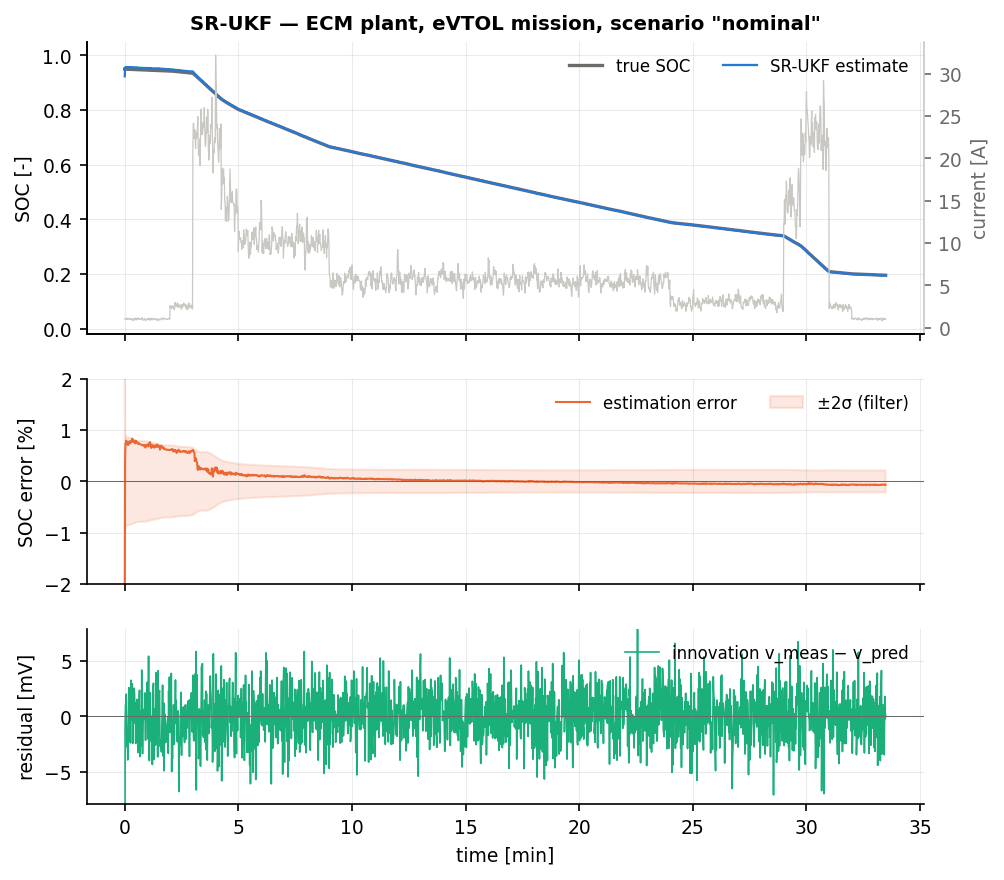
\includegraphics[width=\textwidth]{figures/cell_SRUKF_nominal.png}
\caption{SR-UKF on the nominal eVTOL mission: true and estimated SOC (top), estimation error with the $\pm 2\sigma$ band when available (middle), voltage residual (bottom).}
\end{figure}
\begin{figure}[H]\centering
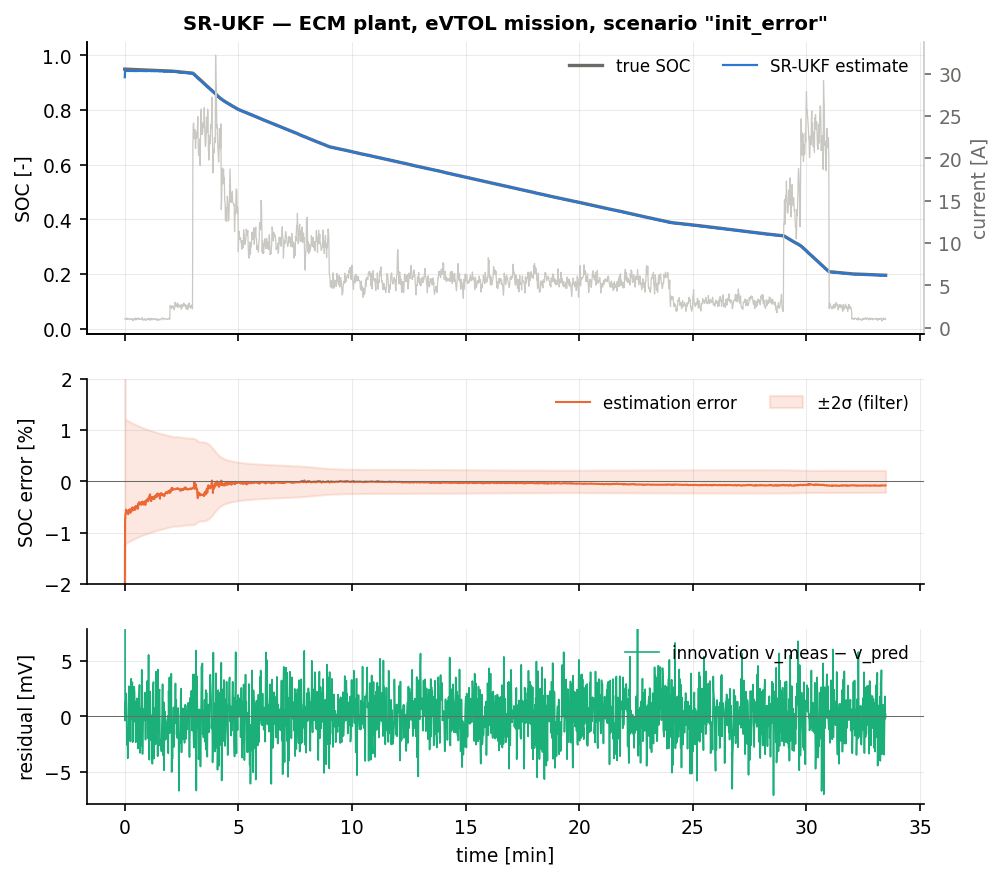
\includegraphics[width=\textwidth]{figures/cell_SRUKF_init_error.png}
\caption{SR-UKF with a 35\,\% initial SOC error.}
\end{figure}

All numbers are three-seed means in per cent SOC.

The SR-UKF reproduces the covariance UKF on all twelve ECM scenarios and all nine SPM scenarios
to two decimals: ECM \texttt{nominal} $0.20/0.04\,\%$, \texttt{init\_error} $0.17/0.07\,\%$
with $t_{\text{conv}} = 0$\,s, \texttt{current\_bias} $0.58/0.57\,\%$, \texttt{cold}
$0.27/0.07\,\%$, \texttt{aged\_cell} $1.10/1.36\,\%$, \texttt{param\_mismatch}
$1.29/1.37\,\%$, \texttt{sensor\_dropout} $1.39/0.86\,\%$, \texttt{preisach} $1.35/0.23\,\%$
($t_{\text{conv}} = 214$\,s), \texttt{combined} $1.23/1.19\,\%$ with $t_{\text{conv}} = 0$\,s.
Element-wise over a full mission the two agree to $\max\abs{\Delta\vx} = 4.1\times10^{-11}$ and
$\max\abs{\Delta\mP} = 2.3\times10^{-12}$ --- three orders of magnitude looser than the
SR-EKF/EKF agreement ($10^{-14}$), which is precisely the signature of the near-cancelling
downdate of Remark~\ref{rm:srukf-downdate}: about one significant digit is lost there, and the
remainder accumulates over $\num{18000}$ steps.

Like the UKF, the SR-UKF is the filter that survives \texttt{combined}: its steady-state
error of $1.19\,\%$ against the EKF's $12.44\,\%$ is the best figure of the fifteen on that
scenario. The reason is the one analysed in Chapter~\ref{ch:ukf}: its
predicted-measurement variance is inflated by the second-order term and the posterior does not
collapse after the first update. All other estimation behaviour --- the mild transient penalty
on \texttt{nominal}, the good \texttt{cold} and \texttt{aged\_cell} results, the degradation on
\texttt{sensor\_dropout} and the slow \texttt{preisach} convergence --- is that of
Chapter~\ref{ch:ukf}.

The cost conclusion differs from the SR-EKF's. There the factored form cost $70\,\%$ more time
for identical answers; here it costs $8\,\%$ ($1.42$--$1.57\,\SI{}{\micro\second}$ against the
covariance UKF's $1.34$--$1.46$), because the covariance UKF's two Cholesky factorisations per
step are exactly what the square-root form avoids. For that price it removes the failure mode
where a marginally indefinite $\mP$ stops the sigma-point generation.

The single-precision build is where this chapter's caveat earns its place. The
float-versus-double table shows the SR-UKF at $0.14\,\%$ on \texttt{nominal} in float32 against
$0.04\,\%$ in double --- a factor of $3.5$, and the largest nominal degradation of any filter in
this family, where the covariance UKF moves only from $0.04$ to $0.05\,\%$. That is the
rank-one downdate of \eqref{eq:srukf-mu2} cancelling $88\,\%$ of the pre-downdate variance
(Remark~\ref{rm:srukf-downdate}): in double the lost significant digit is invisible, in single
precision it is not. Nothing diverges, the errors remain far below the acceptance threshold, and
on the harder scenarios the float build is actually better ($0.96\,\%$ against $1.50\,\%$ on
\texttt{aged\_cell}, $0.23\,\%$ against $1.79\,\%$ on \texttt{combined}) --- but the nominal
number is a genuine warning. If the target is single precision and $\alpha$ must be small, use
$\lambda\ge0$ (see the discussion of the benchmark options above) or the cubature point set,
both of which make every rank-one modification an update rather than a downdate.

\paragraph{SPM plant: structured model error.}
\begin{figure}[H]\centering
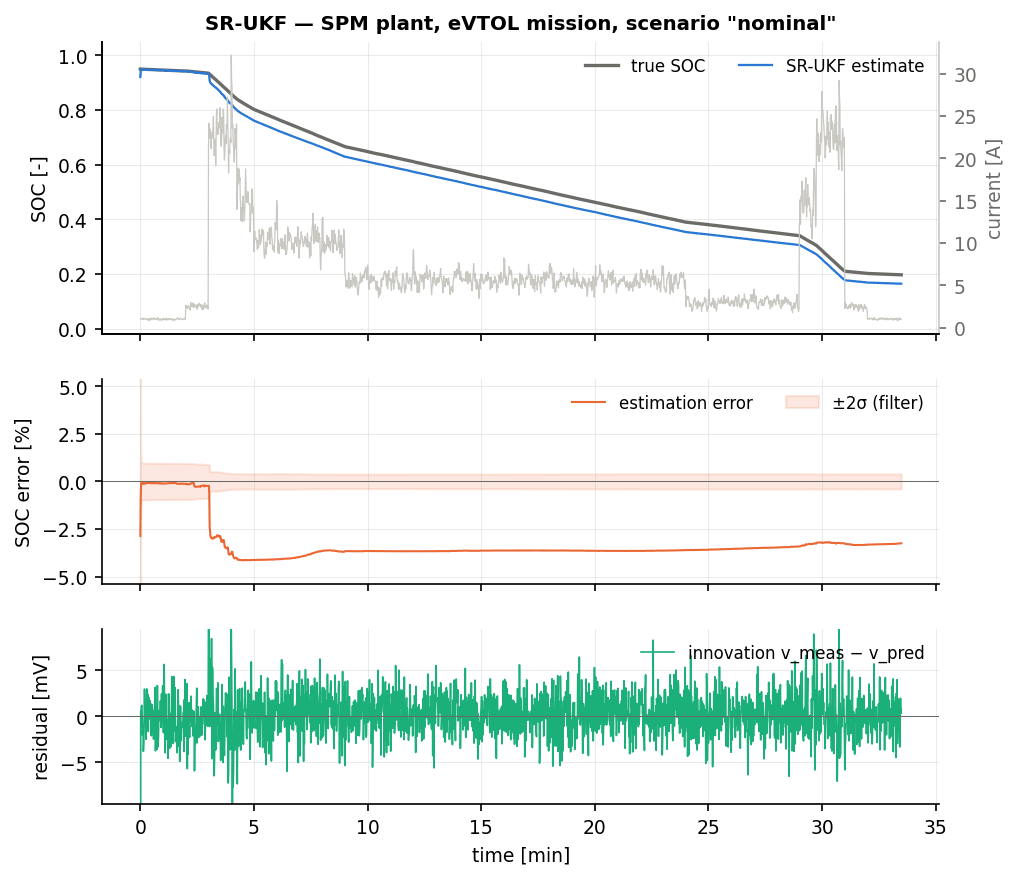
\includegraphics[width=\textwidth]{figures/cellspm_SRUKF_nominal.png}
\caption{SR-UKF on the nominal mission with the electrochemical (SPM) plant; identical to the covariance UKF.}
\end{figure}
The SPM block of the table is a different kind of test. The plant is the electrochemical
single-particle model; the estimator still runs a 2-RC equivalent circuit, fitted to that plant,
which leaves a \emph{structured} residual of about $4$\,mV (Butler--Volmer kinetics and
solid-phase diffusion that no 2-RC circuit can reproduce) and a slow second branch,
$\tau_2 = 556$\,s. Over a $33$-minute mission a $556$\,s pole barely relaxes, so $v_2(t)$ is
close to an affine ramp --- and so is $\ocv(\soc(t))$ while the cell discharges at a roughly
constant rate. The two channels through which the measurement sees the state,
$(\partial\ocv/\partial\soc)\,\delta\soc$ and $-\delta v_2$, are therefore nearly collinear in
the information accumulated over the flight: the pair $(\soc, v_2)$ is close to unobservable,
and no filter can decide whether a persistent few-millivolt residual belongs to the slow RC
branch or to the state of charge. Because that direction is weakly observable, a $4$\,mV
structured error maps onto \emph{several per cent} of SOC instead of the
$4\,\text{mV}/0.8\,\text{V}\approx0.5\,\%$ a well-conditioned channel would give. This
$(\soc,v_2)$ ambiguity, not the size of the residual, is the mechanism behind the
$3.7$--$4.6\,\%$ band in which the whole classical family sits.

The SR-UKF's SPM rows are the UKF's: $3.95/3.96\,\%$ on \texttt{nominal}, $8.29\,\%$ on
\texttt{cold}, $6.46\,\%$ on \texttt{current\_bias}, $7.26\,\%$ on \texttt{sensor\_dropout},
$4.95\,\%$ on \texttt{param\_mismatch}, $1.76\,\%$ on \texttt{outliers}. They sit slightly above
the EKF's ($3.73$, $7.35$, $5.69$, $5.31$, $3.13$, $1.99\,\%$), because a statistical
regression over the prior weights the ill-conditioned OCV channel more heavily than a tangent
does. Nothing diverges. It is worth noting for a square-root chapter that the SPM rows are the
only place in this report where the filters are visibly \emph{mis-specified}, and that the
covariance form remained positive definite there too: a structurally wrong model stresses the
estimator statistically, not numerically, so the factorisation neither helps nor hurts.

\section{Summary}
The square-root UKF is the form in which the unscented filter should be implemented: the same
estimates as the covariance UKF, guaranteed positive semi-definite $\mP$, no per-step
factorisation, and on this benchmark a time penalty of under $10\,\%$. The one caution --- and
the float results make it concrete --- is the rank-one downdate of the centre point, which with
a small $\alpha$ nearly cancels the QR result and costs roughly one significant digit,
visible as a $3.5\times$ nominal degradation in float32. A guarded implementation (fall-back
re-factorisation) makes this safe, and choosing $\lambda\ge0$ removes it entirely at the price
of a wider point spread.

% Copyright 2026 Sreeram Anil
% SPDX-License-Identifier: CC-BY-4.0
% =============================================================================
%  U-D factorised Kalman filter (Bierman-Thornton) — classical Kalman family
% =============================================================================
\chapter{U-D Factorised Kalman Filter (UD-EKF)}
\label{ch:udekf}

\section*{At a glance}
\begin{tabular}{@{}l>{\raggedright\arraybackslash}p{0.76\textwidth}@{}}
Family & classical Kalman (factored) \\
Header & \texttt{include/estkit/filters/udkf.hpp} \\
Registered name & \texttt{UD-EKF} \\
State dimension & $n_x = 4$ (cell model) --- generic in $n_x, n_u, n_y$ \\
Propagated quantities & $\mU$ unit upper triangular, $\mD$ diagonal, $\mP = \mU\mD\mU^\T$ \\
Cost per step & $\mathcal{O}(n_x^2(n_x{+}n_q))$, no square roots; $0.45$--$0.49\,\SI{}{\micro\second}$/step \\
Primary references & \cite{bierman1977,thornton1976ud,kaminski1971,grewal2014,verhaegen1986} \\
\end{tabular}

\section{Motivation and aerospace/BMS relevance}
The U-D filter is the square-root filter without the square roots. Bierman observed that the
numerical benefit of factoring $\mP$ comes from working with a factor whose condition number
is $\sqrt{\kappa(\mP)}$, and that a Cholesky factor is not the only such object: the
factorisation $\mP = \mU\mD\mU^\T$, with $\mU$ unit upper triangular and $\mD$ diagonal and
non-negative, has the same conditioning and needs only multiplies and divides. On the
fixed-point and early floating-point machines of the 1970s that was decisive, and the
Bierman--Thornton pair (scalar measurement update~\cite[Ch.~V]{bierman1977}, modified weighted
Gram--Schmidt time update~\cite{thornton1976ud}) became the standard formulation for JPL deep
space navigation, for GPS receivers, and for the Space Shuttle navigation filter. It is still
the reference implementation in Grewal and Andrews~\cite{grewal2014} and remains the
formulation most often found in certified embedded navigation software.

For a BMS the argument is the same as for the square-root EKF, with one addition: many
automotive and aerospace battery controllers still use fixed-point DSP cores or software
floating point, where a square root costs tens of cycles. The U-D filter has exactly one
division per state per scalar measurement and no transcendental operations at all.

\section{Problem statement and assumptions}
Model \eqref{eq:ekf-proc}--\eqref{eq:ekf-meas}. The filter maintains
\begin{equation}
\mP = \mU\mD\mU^\T, \qquad
\mU = \begin{bmatrix}1 & u_{12} & \cdots\\ 0 & 1 & \\ & & \ddots\end{bmatrix},\quad
\mD = \diag(d_1,\dots,d_{n_x}),\; d_i\ge0 .
\label{eq:ud-def}
\end{equation}
The measurement update processes one scalar component at a time. For that to be exact rather
than approximate, the measurement noise of the components must be independent; when $\mR$ is
not diagonal the components are first decorrelated (below). No positive-definiteness
assumption is needed beyond $\mD\succeq0$, which the algorithm preserves by construction.

\section{Derivation}
\paragraph{U-D factorisation.} For a symmetric positive semi-definite $\bm{M}$, comparing
entries of $\bm{M} = \mU\mD\mU^\T$ from the bottom-right corner upwards gives the recursion
\begin{equation}
d_j = m_{jj} - \sum_{k>j} u_{jk}^2 d_k, \qquad
u_{ij} = \frac{1}{d_j}\left(m_{ij} - \sum_{k>j} u_{ik}\,d_k\,u_{jk}\right), \quad i<j,
\label{eq:ud-factor}
\end{equation}
processed for $j = n_x, n_x-1,\dots,1$~\cite[App.~III]{bierman1977}. It costs
$\mathcal{O}(n_x^3/6)$ and no square roots.

\paragraph{Bierman's scalar measurement update.} Let the scalar observation be
$y = \bm a^\T\vx + v$, $\Var{v} = r$. Substituting $\mP = \mU\mD\mU^\T$ into the Kalman update
and requiring the result to be in U-D form again yields a recursion in which the innovation
variance is built up one state at a time. With
\begin{equation}
\bm f = \mU^\T\bm a \;(\text{so } f_j = \sum_{i\le j} u_{ij}a_i), \qquad
\bm b = \mD\bm f \;(\text{so } b_j = d_j f_j),
\label{eq:ud-fb}
\end{equation}
set $\alpha_0 = r$ and, for $j = 1,\dots,n_x$,
\begin{align}
\alpha_j &= \alpha_{j-1} + f_j b_j, &
d_j &\leftarrow d_j\,\frac{\alpha_{j-1}}{\alpha_j}, &
\lambda_j &= -\frac{f_j}{\alpha_{j-1}},
\label{eq:ud-bierman1}\\
u_{ij} &\leftarrow u_{ij} + \lambda_j b_i, &
b_i &\leftarrow b_i + u_{ij}^{\text{old}}\,b_j, & &\quad i<j .
\label{eq:ud-bierman2}
\end{align}
After the sweep, two identities hold and are the reason the algorithm works:
\begin{equation}
\alpha_{n_x} = \bm a^\T\mP\bm a + r = \mS \quad\text{(innovation variance)},\qquad
\bm b = \mP\bm a \quad\text{(unnormalised gain)},
\label{eq:ud-identities}
\end{equation}
so the state update is $\xhat \leftarrow \xhat + (\bm b/\alpha_{n_x})(y - \bm a^\T\xhat)$. The
updated $\mU,\mD$ are produced in place. Every $\alpha_j$ is a sum of non-negative terms
($f_jb_j = d_jf_j^2 \ge 0$) added to $r>0$, so no cancellation can make it non-positive: the
update cannot produce a negative variance. The cost is $\mathcal{O}(n_x^2)$ per scalar
measurement with exactly $n_x$ divisions.

\paragraph{Decorrelation for vector measurements.} If $\mR$ is not diagonal, factor
$\mR = \mL_R\mL_R^\T$ and replace $(\mH,\bm\veps)$ by
$(\mL_R\inv\mH,\ \mL_R\inv\bm\veps)$; the transformed components have unit, independent
variances and \eqref{eq:ud-bierman1}--\eqref{eq:ud-bierman2} applies to each in turn with
$r=1$~\cite[\S V.4]{bierman1977}. When components are processed sequentially the state moves
between them, so the $k$-th residual must be taken at the \emph{current} state,
$\delta z_k = \tilde\veps_k - \tilde{\bm a}_k^\T(\xhat - \xminus)$, which for a linearised
model makes sequential processing exactly equivalent to a simultaneous vector update.

\paragraph{Thornton's modified weighted Gram--Schmidt time update.} Write
$\mQ = \mG\mD_q\mG^\T$ (itself a U-D factorisation, so a fully correlated $\mQ$ is admissible)
and stack
\begin{equation}
\mW = \left[\ \mF\mU \;\;\; \mG\ \right] \in \real^{n_x\times(n_x+n_q)}, \qquad
\mD_w = \diag\!\left(\mD,\ \mD_q\right),
\label{eq:ud-thornton-setup}
\end{equation}
so that $\Pminus = \mW\mD_w\mW^\T$. Applying \emph{weighted} Gram--Schmidt to the ROWS of
$\mW$, orthogonalising from the last row upwards, gives
\begin{equation}
d^-_i = \sum_k W_{ik}^2 (\mD_w)_k, \qquad
u^-_{ji} = \frac{1}{d^-_i}\sum_k W_{ik}(\mD_w)_k W_{jk}, \qquad
W_{j:} \leftarrow W_{j:} - u^-_{ji}W_{i:}, \quad j<i,
\label{eq:ud-thornton}
\end{equation}
for $i = n_x,\dots,1$. Because row $i$ is finalised before it is used to reduce rows $j<i$,
the original array satisfies $\mW_{\text{orig}} = \mU^-\mW_{\text{final}}$ with
$\mU^-$ unit upper triangular, and the rows of $\mW_{\text{final}}$ are $\mD_w$-orthogonal
with $\mD_w$-norms $d^-_i$; hence
$\Pminus = \mW_{\text{orig}}\mD_w\mW_{\text{orig}}^\T = \mU^-\mD^-\mU^{-\T}$ as
required~\cite{thornton1976ud}. Cost: $\mathcal{O}(n_x^2(n_x+n_q))$, again with no square
roots.

\section{Algorithm}
\begin{algorithm}[H]
\caption{UD-EKF (Bierman--Thornton) --- one sampling period}
\begin{algorithmic}[1]
\Require $\xplus_{k-1},\mU^+_{k-1},\mD^+_{k-1},\vu_{k-1},\vy_k,\vu_k$
\State \textbf{Time update (Thornton):} $\mF\gets\partial f/\partial\vx|_{\xplus_{k-1},\vu_{k-1}}$;\;
       $\xminus_k\gets f(\xplus_{k-1},\vu_{k-1})$
\State $(\mG,\mD_q)\gets\text{UD}(\mQ)$;\;
       $\mW\gets[\mF\mU^+_{k-1}\;\;\mG]$;\; $\mD_w\gets\diag(\mD^+_{k-1},\mD_q)$
\For{$i=n_x$ \textbf{down to} $1$}
  \State $d^-_i\gets\sum_k W_{ik}^2(\mD_w)_k$
  \For{$j=1,\dots,i-1$}
    \State $u^-_{ji}\gets\left(\sum_k W_{ik}(\mD_w)_kW_{jk}\right)/d^-_i$;\;
           $W_{j:}\gets W_{j:}-u^-_{ji}W_{i:}$
  \EndFor
\EndFor
\State \textbf{Predicted measurement:} $\yhat_k\gets h(\xminus_k,\vu_k)$
\State \textbf{Measurement update (Bierman):} $\mH\gets\partial h/\partial\vx|_{\xminus_k,\vu_k}$;\;
       decorrelate if $\mR$ is not diagonal
\For{$k'=1,\dots,n_y$}
  \State $\bm a\gets$ row $k'$ of $\mH$;\; $\delta z\gets\tilde\veps_{k'}-\bm a^\T(\xhat-\xminus_k)$
  \State apply \eqref{eq:ud-fb}--\eqref{eq:ud-bierman2};\;
         $\xhat\gets\xhat+(\bm b/\alpha_{n_x})\,\delta z$
\EndFor
\State \textbf{if} constraints enabled \textbf{then} $\xplus_k\gets\Pi(\xhat)$
\Ensure $\xplus_k,\mU^+_k,\mD^+_k$ \quad ($\mP$ reconstructed on demand as $\mU\mD\mU^\T$)
\end{algorithmic}
\end{algorithm}

\section{Application to the battery model}
$n_y=1$, so the Bierman sweep runs once per sample: four multiplies for $\bm f = \mU^\T\bm a$,
four for $\bm b$, then four iterations of \eqref{eq:ud-bierman1}--\eqref{eq:ud-bierman2} ---
about $40$ multiply-accumulates and $4$ divisions in total. $\mF$ is diagonal, so
$\mF\mU$ is a row scaling. $\mQ$ is \emph{not} diagonal (it carries the rank-one
current-noise term $\bm b\bm b^\T\sigma_i^2$), which is exactly the case Thornton's algorithm
was designed for: the U-D factorisation of $\mQ$ supplies $\mG$ and $\mD_q$ and the
Gram--Schmidt pass handles the correlation without any special casing. The work array $\mW$ is
$4\times8$.

Options: \code{decorrelate = true} (inactive at $n_y=1$), \code{apply\_constraints = true},
\code{q\_scale = r\_scale = 1}, \code{d\_floor = 0} (a lower bound that can be raised to keep
the filter from becoming arbitrarily confident in a state).

\section{Implementation notes}
The U-D filter is the fastest of the EKF-equivalent implementations, at
$0.45$--$0.49\,\SI{}{\micro\second}$ per step against the square-root EKF's $0.78$--$0.83$ and
the information filter's $1.17$--$1.24$, and indistinguishable from the conventional EKF's
$0.44$--$0.48$: it replaces two Householder QRs by one Gram--Schmidt pass and one scalar sweep
and uses no square roots at all. Only the frozen-linearisation LKF ($320$--$336$\,ns) is
faster, and it is a different estimator. That the factored form costs nothing relative to the
conventional one is the historical selling point of the formulation, and it survives unchanged
on modern hardware.

Numerical guards: $d_j$ is clamped to $\ge$ \code{d\_floor} after each update; an
$\alpha_j$ that fails to be positive (possible only through a corrupted $d_j$) leaves the
state untouched for that index; the gain application is skipped if $\delta z/\alpha$ is not
finite. The U-D factorisation \eqref{eq:ud-factor} sets $d_j = 0$ and $u_{ij} = 0$ rather than
dividing by a non-positive pivot. $\mP$ is exposed through a cached $\mU\mD\mU^\T$ product for
the benchmark's $\sigma_\soc$ reporting; a flight implementation would read
$\sigma_\soc^2 = \sum_j u_{1j}^2 d_j$ directly.
\code{sizeof(UdKf<EcmModel>)} is 4480\,bytes.

Verification: the U-D factorisation was checked against a dense reconstruction
($\max\abs{\mU\mD\mU^\T-\bm{M}} = 2.2\times10^{-16}$ on a $4\times4$ test matrix), and the
complete filter against the EKF over a full mission.

\section{Benchmark results}
\input{tables/cell_UDEKF.tex}
\begin{figure}[H]\centering
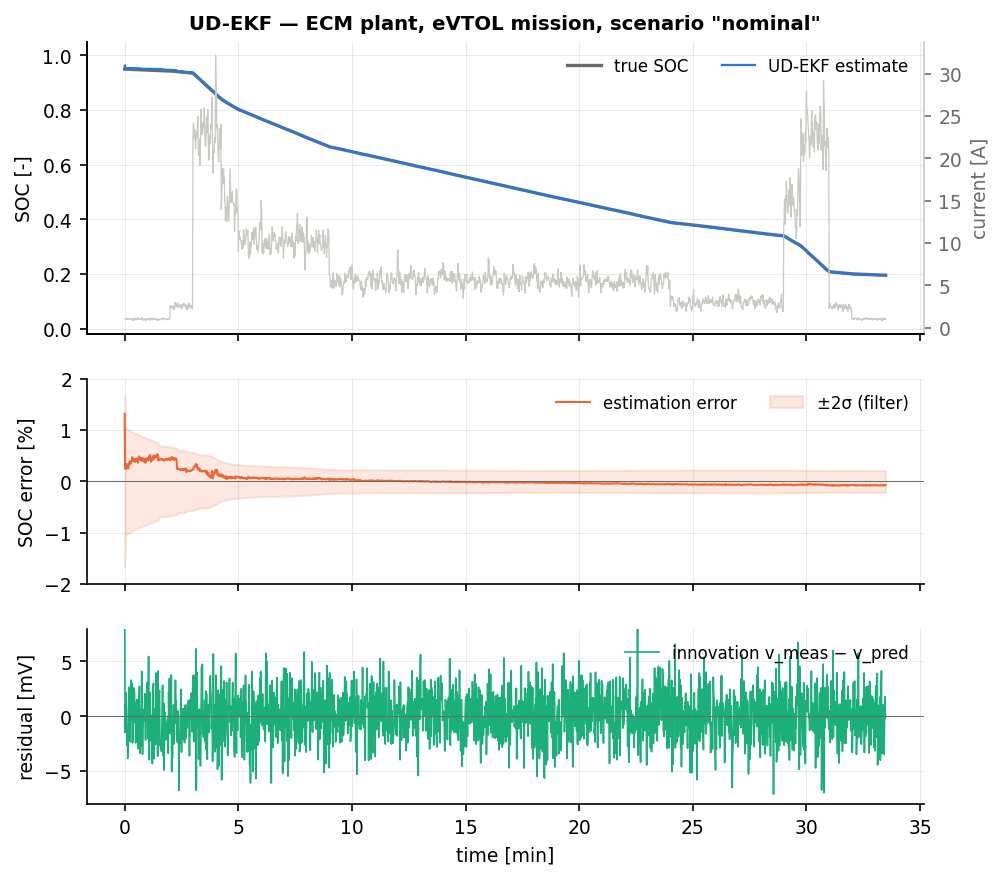
\includegraphics[width=\textwidth]{figures/cell_UDEKF_nominal.png}
\caption{UD-EKF on the nominal eVTOL mission: true and estimated SOC (top), estimation error with the $\pm 2\sigma$ band when available (middle), voltage residual (bottom).}
\end{figure}
\begin{figure}[H]\centering
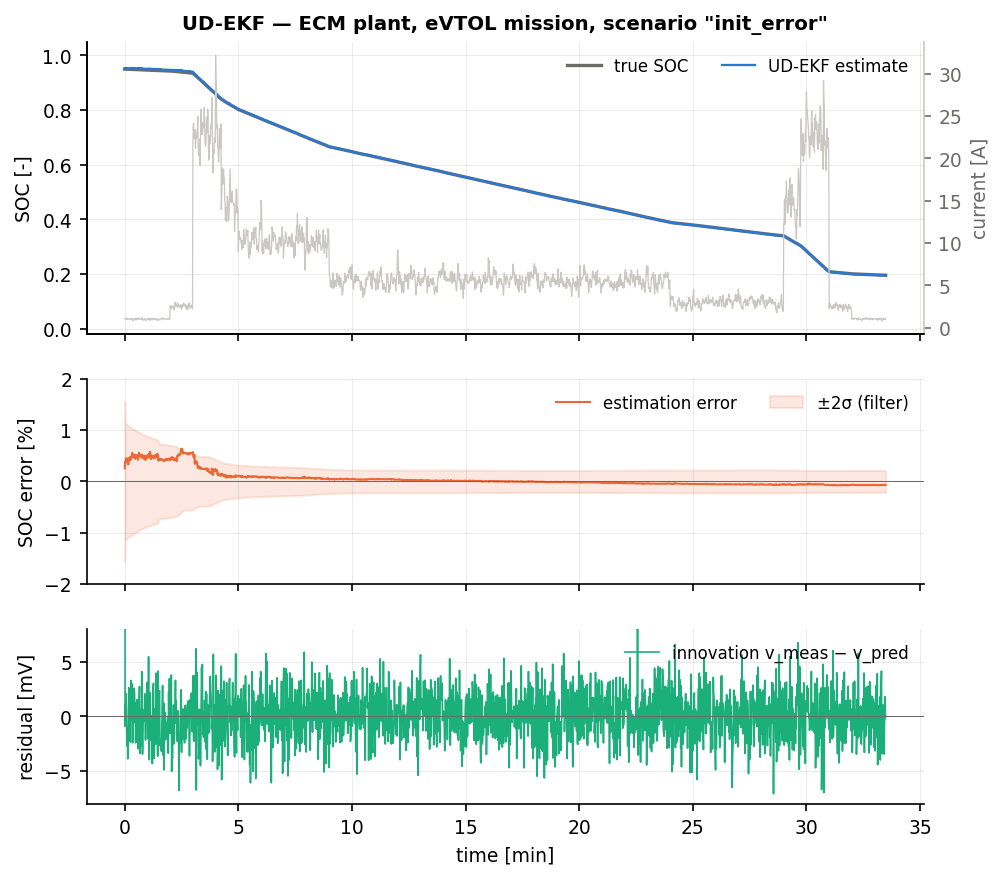
\includegraphics[width=\textwidth]{figures/cell_UDEKF_init_error.png}
\caption{UD-EKF with a 35\,\% initial SOC error.}
\end{figure}

All numbers are three-seed means in per cent SOC.

The UD-EKF reproduces the EKF on all twelve ECM scenarios to two decimals --- \texttt{nominal}
$0.15/0.05\,\%$, \texttt{init\_error} $0.14/0.05\,\%$ with $t_{\text{conv}} = 0$\,s,
\texttt{current\_bias} $0.54/0.61\,\%$, \texttt{outliers} $0.52/0.21\,\%$, \texttt{aged\_cell}
$1.18/1.52\,\%$, \texttt{param\_mismatch} $1.28/1.36\,\%$, \texttt{sensor\_dropout}
$0.72/0.46\,\%$, \texttt{preisach} $0.58/0.20\,\%$, \texttt{combined} $16.02/12.44\,\%$ (never
converges) --- with an element-wise agreement of $\max\abs{\Delta\vx} = 1.6\times10^{-14}$ and
$\max\abs{\Delta\mP} = 7.6\times10^{-16}$ over $\num{18000}$ steps. The covariance agreement is
the tightest of the three EKF-equivalent implementations in this family (SR-EKF
$4.0\times10^{-15}$, EIF $1.3\times10^{-14}$), which is consistent with the U-D form never
forming $\mP$ and never taking a square root. The estimation discussion of
Chapter~\ref{ch:ekf} applies unchanged.

What distinguishes this chapter from the SR-EKF's is the cost column. The U-D filter is
\emph{free} relative to the conventional covariance form --- $0.45$--$0.49\,\SI{}{\micro\second}$
against the EKF's $0.44$--$0.48$, a difference of a few nanoseconds and well inside the
run-to-run spread --- while providing the guarantee that $\mP$ cannot go indefinite
($\mD\succeq0$ is enforced elementwise). The square-root EKF costs $70\,\%$ more for the same
guarantee. There is, on this evidence, no reason to prefer the conventional covariance EKF over
the U-D form in an embedded implementation: it costs the same, is better conditioned, needs no
square roots, and produces the same numbers. In single precision the two are also
indistinguishable ($0.06\,\%$ on \texttt{nominal}, $1.48\,\%$ on \texttt{aged\_cell},
$12.18\,\%$ on \texttt{combined} against the EKF's $12.21\,\%$).

Two caveats. First, the advantage is specific to $n_y\ll n_x$: the Bierman sweep costs
$\mathcal{O}(n_x^2)$ per scalar measurement, so with many simultaneous measurements the
$\mathcal{O}(n_yn_x^2)$ total overtakes a single batched update; the square-root array form of
Chapter~\ref{ch:srekf} handles a vector measurement in one pass and is preferable there.
Second, in the artificial ill-conditioning stress test described in Chapter~\ref{ch:srekf}
(float build, $\mR$ scaled by $10^{-4}$) the U-D filter came out at
$\text{RMSE}_{\text{ss}} = 5.07\,\%$ against the SR-EKF's $0.79\,\%$ and the EKF's $2.39\,\%$;
since all three are algebraically identical this reflects the chaotic sensitivity of that
deliberately broken configuration rather than a conditioning ranking, and no conclusion should
be drawn from it beyond ``do not trust a filter whose $\mR$ is wrong by four orders of
magnitude''.

\paragraph{SPM plant: structured model error.}
\begin{figure}[H]\centering
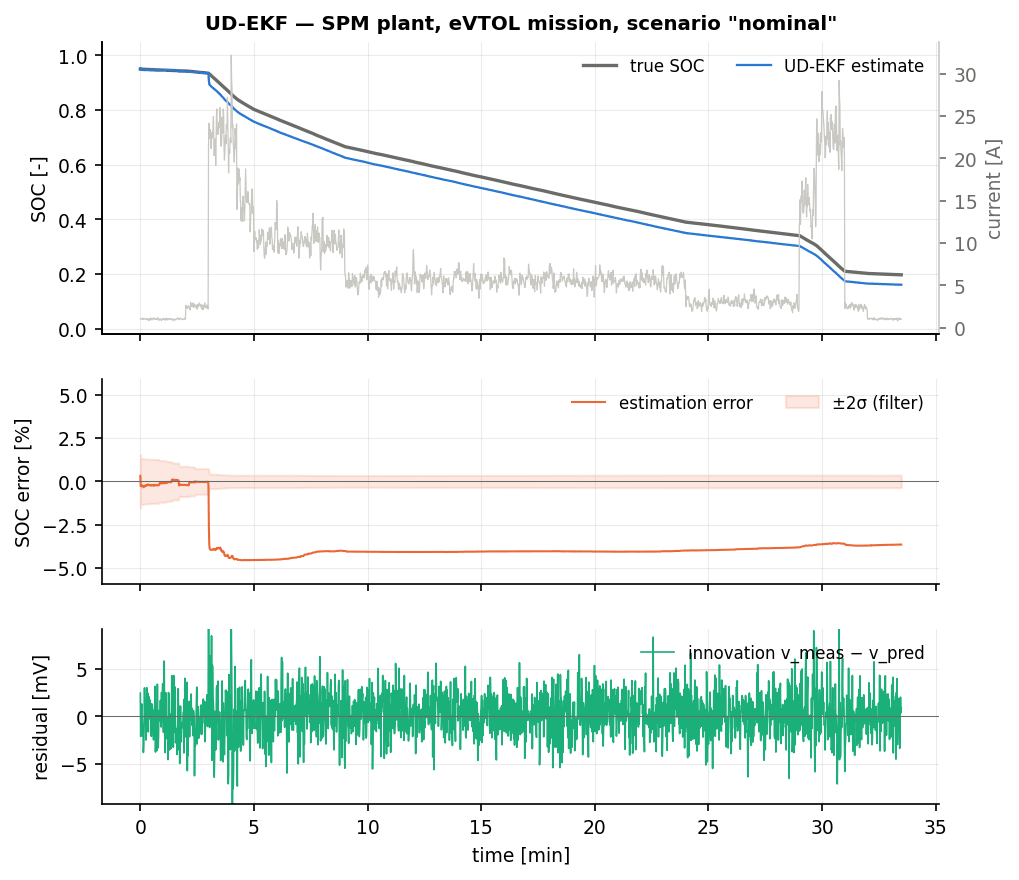
\includegraphics[width=\textwidth]{figures/cellspm_UDEKF_nominal.png}
\caption{UD-EKF on the nominal mission with the electrochemical (SPM) plant; identical to the conventional EKF.}
\end{figure}
The SPM block of the table is a different kind of test. The plant is the electrochemical
single-particle model; the estimator still runs a 2-RC equivalent circuit, fitted to that plant,
which leaves a \emph{structured} residual of about $4$\,mV (Butler--Volmer kinetics and
solid-phase diffusion that no 2-RC circuit can reproduce) and a slow second branch,
$\tau_2 = 556$\,s. Over a $33$-minute mission a $556$\,s pole barely relaxes, so $v_2(t)$ is
close to an affine ramp --- and so is $\ocv(\soc(t))$ while the cell discharges at a roughly
constant rate. The two channels through which the measurement sees the state,
$(\partial\ocv/\partial\soc)\,\delta\soc$ and $-\delta v_2$, are therefore nearly collinear in
the information accumulated over the flight: the pair $(\soc, v_2)$ is close to unobservable,
and no filter can decide whether a persistent few-millivolt residual belongs to the slow RC
branch or to the state of charge. Because that direction is weakly observable, a $4$\,mV
structured error maps onto \emph{several per cent} of SOC instead of the
$4\,\text{mV}/0.8\,\text{V}\approx0.5\,\%$ a well-conditioned channel would give. This
$(\soc,v_2)$ ambiguity, not the size of the residual, is the mechanism behind the
$3.7$--$4.6\,\%$ band in which the whole classical family sits.

Being algebraically the EKF, this filter inherits the EKF's SPM rows exactly:
$3.65/3.73\,\%$ on \texttt{nominal} with a voltage residual of only $1.02$\,mV,
$7.35\,\%$ on \texttt{cold}, $5.69\,\%$ on \texttt{current\_bias}, $5.31\,\%$ on
\texttt{sensor\_dropout}, $3.13\,\%$ on \texttt{param\_mismatch} and $1.99\,\%$ on
\texttt{outliers}. Fitting the voltage to a millivolt while being $4\,\%$ wrong about SOC is
the signature of the ambiguity: the filter pays for the fit with $v_2$ and $\soc$ in the wrong
proportion. Nothing diverges and $t_{\text{conv}} = 0$ on every SPM row --- the error is a
bias, not a drift. Within the family the tangent-linearising filters (EKF, IEKF and these three
re-implementations) are at the \emph{good} end of the band, because a tangent commits less
weight to the badly conditioned OCV channel than a wide statistical regression does; only the
frozen-linearisation LKF ($1.72\,\%$, Chapter~\ref{ch:lkf}) and the second-order EKF
($3.52\,\%$) do better.

\section{Summary}
The Bierman--Thornton U-D filter is the implementation of choice for an embedded EKF: it gives
bit-for-bit the EKF's estimates, guarantees a non-negative covariance by construction, uses no
square roots and no matrix inversions, and on this benchmark costs exactly what the conventional
EKF costs. Use it for any fixed-point or software-floating-point target, for any application
where a negative variance must be impossible by construction, and by default whenever
$n_y\ll n_x$. Its limitation is the scalar measurement sweep, which becomes the bottleneck when
many measurements arrive simultaneously; and, being an EKF, it inherits the EKF's
over-confidence on curved measurement functions (\texttt{combined}) and the EKF's $4\,\%$ bias
under structured model error (the SPM rows).

% Copyright 2026 Sreeram Anil
% SPDX-License-Identifier: CC-BY-4.0
% =============================================================================
%  Extended information filter — classical Kalman family
% =============================================================================
\chapter{Extended Information Filter (EIF)}
\label{ch:eif}

\section*{At a glance}
\begin{tabular}{@{}l>{\raggedright\arraybackslash}p{0.76\textwidth}@{}}
Family & classical Kalman (information form) \\
Header & \texttt{include/estkit/filters/eif.hpp} \\
Registered name & \texttt{EIF} \\
State dimension & $n_x = 4$ (cell model) --- generic in $n_x, n_u, n_y$ \\
Propagated quantities & $\bm{Y} = \mP\inv$, $\bm{\upsilon} = \bm{Y}\xhat$ \\
Cost per step & $\mathcal{O}(n_x^3)$, three $n_x\times n_x$ inversions; $1.17$--$1.24\,\SI{}{\micro\second}$/step \\
Primary references & \cite{mutambara1998,andersonmoore1979,maybeck1979,thrun2005} \\
\end{tabular}

\section{Motivation and aerospace/BMS relevance}
The information filter is the same estimator as the Kalman filter written in terms of the
inverse covariance. This exchanges the difficulty of the two halves of the cycle: the
measurement update becomes a \emph{sum} and the time update becomes the hard part. Three
consequences make the trade worthwhile in specific architectures.

First, additivity. $N$ conditionally independent sensors contribute $N$ terms
$\mH_i^\T\mR_i\inv\mH_i$ that can be computed on separate processors, transmitted, and summed
in any order with no synchronisation. This is the mathematical basis of decentralised and
federated filters~\cite{mutambara1998,carlson1990federated} and is directly relevant to a
battery pack, where dozens of cell-monitoring ASICs each produce a voltage measurement that
must be fused by one master.

Second, ignorance is representable. ``No prior information'' is $\bm{Y} = \bm{0}$ exactly, whereas
a covariance filter must fake it with a large $\mP_0$ and then suffer the numerical
consequences. A BMS that wakes up after a long rest with no stored SOC can start the EIF from
$\bm{Y}=\bm0$ and let the first OCV measurement define the estimate.

Third, sparsity. In large problems (SLAM, pack-level estimation with weak inter-cell
coupling) $\bm{Y}$ is nearly sparse while $\mP$ is dense, which is the basis of the sparse
extended information filter~\cite{thrun2005}. None of these advantages is exercised by a
single-cell, single-sensor benchmark; this chapter therefore serves to \emph{validate} the
information form against the EKF and to quantify what the change of variables costs.

\section{Problem statement and assumptions}
Model \eqref{eq:ekf-proc}--\eqref{eq:ekf-meas}. Define
\begin{equation}
\bm{Y}_k = \mP_k\inv \in\real^{n_x\times n_x} \quad\text{(information matrix)},\qquad
\bm{\upsilon}_k = \bm{Y}_k\xhat_k \in\real^{n_x} \quad\text{(information vector)}.
\label{eq:eif-defs}
\end{equation}
The information form requires $\mP$ to be invertible at all times, hence $\mQ\succ0$; the
time update derived below additionally requires $\mF$ to be invertible, which holds for any
discretisation of a physical system (and here $\mF=\diag(1,a_1,a_2,a_h)$ with all entries in
$(0,1]$).

\section{Derivation}
\paragraph{Measurement update.} Starting from the covariance-form Joseph update and applying
the matrix inversion lemma, or directly from the Gaussian log-density
\begin{equation}
-2\log p(\vx\mid\vy_{1:k}) = (\vx-\xminus_k)^\T(\Pminus_k)\inv(\vx-\xminus_k)
 + (\vy_k-h(\vx,\vu_k))^\T\mR\inv(\vy_k-h(\vx,\vu_k)) + \text{const},
\label{eq:eif-logpost}
\end{equation}
linearising $h$ about $\xminus_k$ and collecting the quadratic and linear terms in $\vx$:
\begin{align}
\bm{Y}^+_k &= \bm{Y}^-_k + \mH_k^\T\mR\inv\mH_k, \label{eq:eif-mu-Y}\\
\bm\upsilon^+_k &= \bm\upsilon^-_k + \mH_k^\T\mR\inv\left[\vy_k - h(\xminus_k,\vu_k) + \mH_k\xminus_k\right].
\label{eq:eif-mu-y}
\end{align}
The bracket is the linearised measurement ``referred back to the origin''; for a linear model
it is simply $\vy_k$. Equations \eqref{eq:eif-mu-Y}--\eqref{eq:eif-mu-y} contain no inverse of
an $n_x\times n_x$ matrix and no gain: the update is an addition of the information supplied
by the sensor, which is why it parallelises trivially.

\paragraph{Time update.} This is where the work moves. In covariance form
$\Pminus_k = \mF\Pplus_{k-1}\mF^\T+\mQ$, so
\begin{equation}
\bm{Y}^-_k = \left[\mF(\bm{Y}^+_{k-1})\inv\mF^\T + \mQ\right]\inv .
\label{eq:eif-tu-naive}
\end{equation}
Define $\bm{M} = \mF^{-\T}\bm{Y}^+_{k-1}\mF\inv$, so that
$\mF(\bm{Y}^+_{k-1})\inv\mF^\T = \bm{M}\inv$. The Woodbury identity
$(\bm{M}\inv+\mQ)\inv = \bm{M} - \bm{M}(\bm{M}+\mQ\inv)\inv\bm{M}$ then gives the standard information-form
time update~\cite[\S6.3]{andersonmoore1979}
\begin{equation}
\boxed{\;\bm{Y}^-_k = \bm{M} - \bm{M}\left(\bm{M} + \mQ\inv\right)\inv\bm{M}, \qquad
 \bm{M} = \mF^{-\T}\bm{Y}^+_{k-1}\mF\inv .\;}
\label{eq:eif-tu}
\end{equation}
For the nonlinear mean the propagation is unchanged, $\xminus_k = f(\xplus_{k-1},\vu_{k-1})$,
and $\bm\upsilon^-_k = \bm{Y}^-_k\xminus_k$. Note the structural asymmetry: the measurement
update needs $\mR\inv$ ($n_y\times n_y$, here a scalar) while the time update needs $\mF\inv$,
$\mQ\inv$ and one $n_x\times n_x$ solve.

\paragraph{Recovering the estimate.} $\xhat_k = \bm{Y}_k\inv\bm\upsilon_k$ and $\mP_k=\bm{Y}_k\inv$.
Because the benchmark adapter needs $\soc$ and $\sigma_\soc$ at every sample, and because the
nonlinear $f$ and $h$ must be evaluated at $\xhat$, the implementation recovers them through a
cached, lazily evaluated inversion: a \code{dirty} flag is set by \code{predict} and
\code{update} and cleared by the first accessor that needs $(\xhat,\mP)$.

\begin{proposition}\label{prop:eif-equiv}
For the same linearisation points, \eqref{eq:eif-mu-Y}--\eqref{eq:eif-tu} produce the same
estimate and covariance as the EKF of Chapter~\ref{ch:ekf}.
\end{proposition}
This is an algebraic identity, and it is verified numerically below; the value of the chapter
is that the identity holds in \emph{practice}, i.e. that the extra inversions do not destroy
it.

\section{Algorithm}
\begin{algorithm}[H]
\caption{EIF --- one sampling period}
\begin{algorithmic}[1]
\Require $\bm{Y}^+_{k-1},\bm\upsilon^+_{k-1},\vu_{k-1},\vy_k,\vu_k$
\State recover $\xplus_{k-1}\gets(\bm{Y}^+_{k-1})\inv\bm\upsilon^+_{k-1}$ if not cached
\State \textbf{Time update:} $\mF\gets\partial f/\partial\vx|_{\xplus_{k-1},\vu_{k-1}}$;\;
       $\xminus_k\gets f(\xplus_{k-1},\vu_{k-1})$
\State $\bm{M}\gets\mF^{-\T}\bm{Y}^+_{k-1}\mF\inv$;\;
       $\bm{Y}^-_k\gets\bm{M}-\bm{M}(\bm{M}+\mQ\inv)\inv\bm{M}$;\;
       $\bm\upsilon^-_k\gets\bm{Y}^-_k\xminus_k$
\State \textbf{(fall-back)} if $\mF$ or $\mQ$ is singular: $\bm{Y}^-_k\gets(\mF\Pplus_{k-1}\mF^\T+\mQ)\inv$
\State \textbf{Predicted measurement:} $\yhat_k\gets h(\xminus_k,\vu_k)$
\State \textbf{Measurement update:} $\mH\gets\partial h/\partial\vx|_{\xminus_k,\vu_k}$
\State $\bm{Y}^+_k\gets\bm{Y}^-_k+\mH^\T\mR\inv\mH$;\;
       $\bm\upsilon^+_k\gets\bm\upsilon^-_k+\mH^\T\mR\inv(\vy_k-\yhat_k+\mH\xminus_k)$
\State $\Pplus_k\gets(\bm{Y}^+_k)\inv$;\; $\xplus_k\gets\Pplus_k\bm\upsilon^+_k$
\State \textbf{if} constraints enabled \textbf{then} $\xplus_k\gets\Pi(\xplus_k)$, $\bm\upsilon^+_k\gets\bm{Y}^+_k\xplus_k$
\Ensure $\bm{Y}^+_k,\bm\upsilon^+_k$ (and the cached $\xplus_k,\Pplus_k$)
\end{algorithmic}
\end{algorithm}

\section{Application to the battery model}
Because $\mF=\diag(1,a_1(T),a_2(T),a_h(i))$ the inverse $\mF\inv$ is a diagonal reciprocal and
$\bm{M} = \mF^{-\T}\bm{Y}\mF\inv$ costs $n_x^2$ divisions instead of two matrix products --- a
diagonal $\mF$ is the best case for the information form. $\mQ$, in contrast, is
\emph{not} diagonal: it is $\bm b\bm b^\T\sigma_i^2 + \diag(q_{\text{floor}}^2)$, a rank-one
current-noise term plus a floor, so $\mQ\inv$ is a genuine $4\times4$ inverse. (A
Sherman--Morrison update on the rank-one part would reduce this to $\mathcal{O}(n_x^2)$; it is
not implemented because the generic model interface only exposes $\mQ$ itself.)

With $n_y=1$ the measurement update is $\mH^\T\mH/R$ --- a rank-one addition, four multiplies
--- which is a good illustration of the information form's asymmetry: what a covariance filter
does with an inverse and a gain, the information filter does with an outer product.

Options: \code{information\_time\_update = true} (use \eqref{eq:eif-tu}; setting it to
\code{false} selects the covariance-form fall-back and gives identical results),
\code{apply\_constraints = true}, \code{q\_scale = r\_scale = 1}.

\section{Implementation notes}
Three $4\times4$ inversions per step ($\mF\inv$, $\mQ\inv$, $(\bm{Y}^+)\inv$) plus one SPD solve
explain the measured $1.17$--$1.24\,\SI{}{\micro\second}$ against the EKF's
$0.44$--$0.48\,\SI{}{\micro\second}$: on this problem the information form costs $2.6\times$ an
EKF step and buys nothing, because there is one sensor and $\bm{Y}$ is dense.
The break-even point is the number of independent measurement channels: the covariance form
costs $\mathcal{O}(n_y^3)$ in the update, the information form $\mathcal{O}(n_x^3)$ in the
prediction, so the information form wins once $n_y\gtrsim n_x$ --- which is exactly the
pack-level situation.

Robustness: $\bm{Y}_0 = \mP_0\inv$ is replaced by $10^6\mI$ if $\mP_0$ is singular;
\eqref{eq:eif-tu} is attempted first and silently falls back to
$(\mF\Pplus\mF^\T+\mQ)\inv$ if either $\mF$ or $\mQ$ is numerically singular; the cached
$(\xhat,\mP)$ are only updated when the inversion succeeds, so a failed inversion leaves the
last good estimate in place rather than producing NaN. After constraint projection the
information vector is recomputed as $\bm\upsilon = \bm{Y}\xhat$ to keep the pair consistent.
\code{sizeof(Eif<EcmModel>)} is 4472\,bytes.

\section{Benchmark results}
\input{tables/cell_EIF.tex}
\begin{figure}[H]\centering
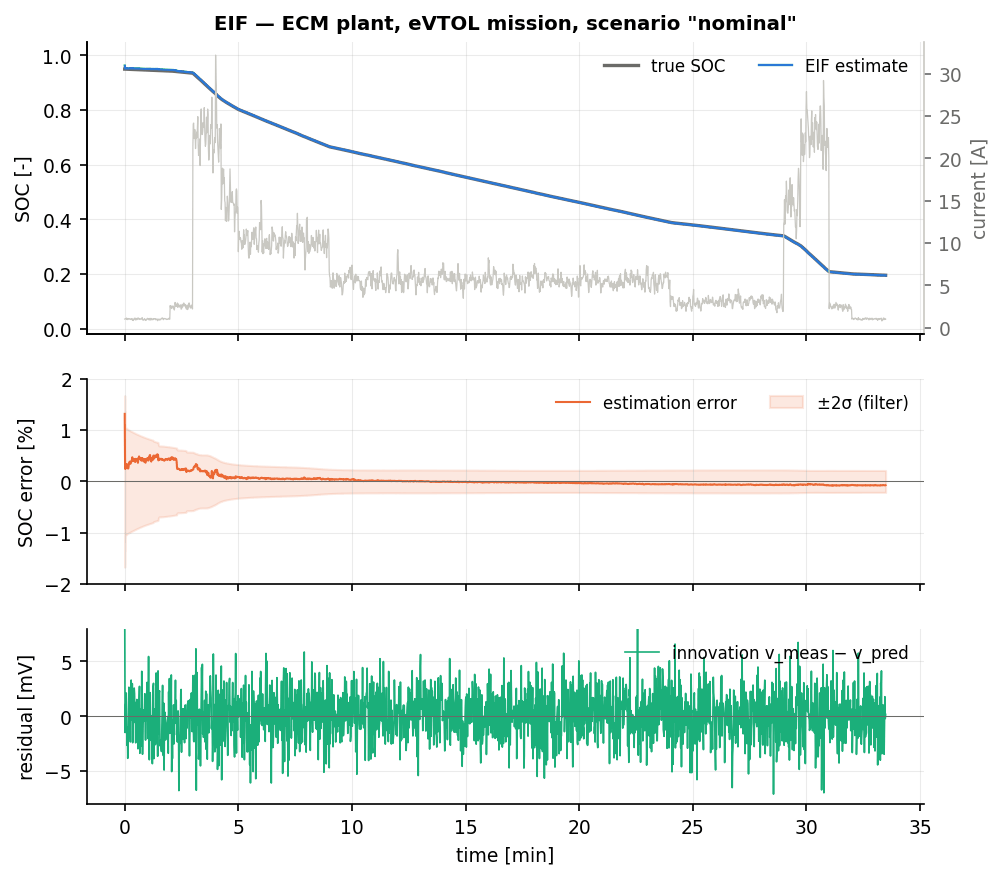
\includegraphics[width=\textwidth]{figures/cell_EIF_nominal.png}
\caption{EIF on the nominal eVTOL mission: true and estimated SOC (top), estimation error with the $\pm 2\sigma$ band when available (middle), voltage residual (bottom).}
\end{figure}
\begin{figure}[H]\centering
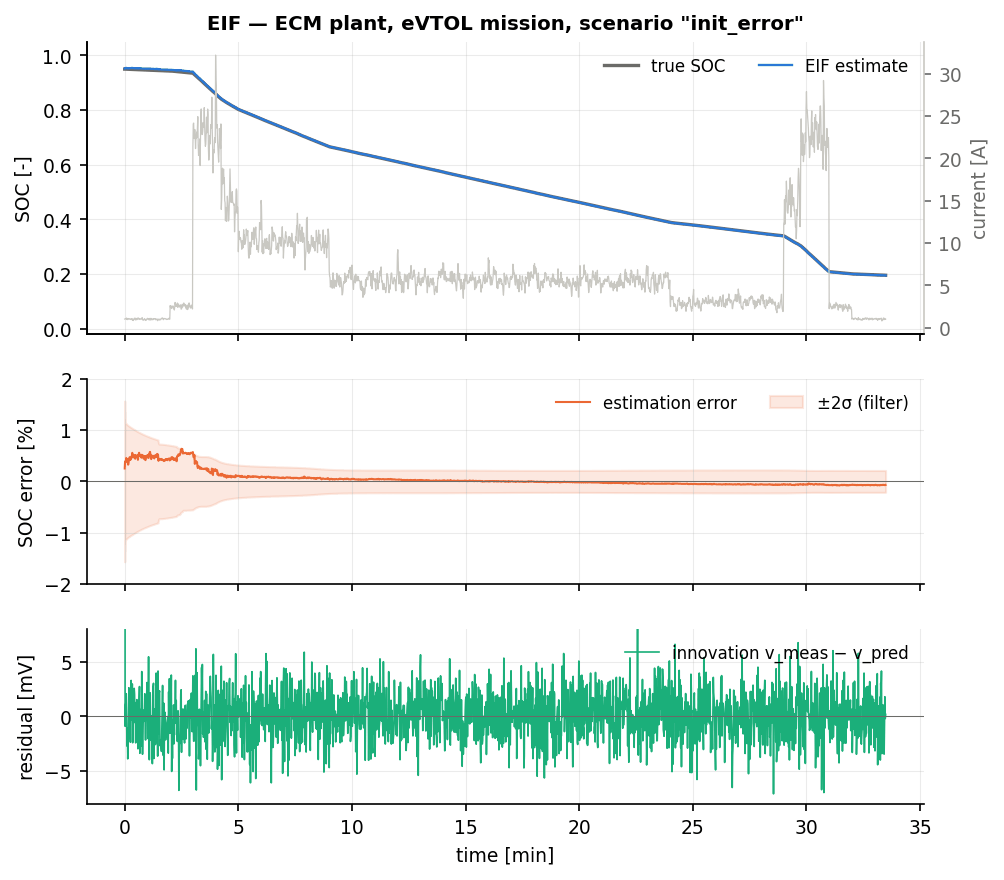
\includegraphics[width=\textwidth]{figures/cell_EIF_init_error.png}
\caption{EIF with a 35\,\% initial SOC error.}
\end{figure}

All numbers are three-seed means in per cent SOC.

The EIF reproduces the EKF exactly on every scenario of both plants, to all printed decimals:
ECM \texttt{nominal} $0.15/0.05\,\%$, \texttt{init\_error} $0.14/0.05\,\%$ with
$t_{\text{conv}} = 0$\,s, \texttt{current\_bias} $0.54/0.61\,\%$, \texttt{aged\_cell}
$1.18/1.52\,\%$, \texttt{param\_mismatch} $1.28/1.36\,\%$, \texttt{sensor\_dropout}
$0.72/0.46\,\%$, \texttt{preisach} $0.58/0.20\,\%$, \texttt{combined} $16.02/12.44\,\%$. A
direct element-wise comparison over a full nominal mission ($\num{18000}$ steps) gives
$\max\abs{\Delta\vx} = 1.9\times10^{-11}$ and $\max\abs{\Delta\mP} = 1.3\times10^{-14}$,
confirming Proposition~\ref{prop:eif-equiv} numerically. The discussion of
Chapter~\ref{ch:ekf} therefore applies without change, including the \texttt{combined} failure.

The $10^{-11}$ discrepancy is larger than the $10^{-14}$ of the square-root and U-D filters
(Chapters~\ref{ch:srekf}, \ref{ch:udekf}) --- a small but real indication that the information
form is the \emph{least} numerically favourable of the algebraically equivalent
implementations. That is expected: it squares the condition number twice over (once in
$\bm{Y} = \mP\inv$, once in $(\bm{M}+\mQ\inv)\inv$) where a square-root filter halves it. The
single-precision build shows the same tendency at the level of the estimates: on
\texttt{combined} the EIF gives $12.66\,\%$ in float against $11.90\,\%$ in double, the largest
float-double gap of the four EKF-equivalent implementations (EKF $12.21$, SR-EKF $12.21$,
UD-EKF $12.18\,\%$), while on \texttt{nominal} it is $0.03\,\%$ against $0.06\,\%$ --- noise, at
this level. At $n_x = 4$ the effect is still below the estimation error; at larger $n_x$ or with
near-deterministic states ($\mQ\to0$, where $\mQ\inv$ blows up) it would not be.

The cost, $1.17$--$1.24\,\SI{}{\micro\second}$ against the EKF's $0.44$--$0.48$ --- a factor of
$2.6$ --- is the price of the change of variables on a single-sensor problem. It is worth
restating that this is the worst case for the information form: with one measurement channel and
a dense $\mQ$, every structural advantage is absent.

\paragraph{SPM plant: structured model error.}
\begin{figure}[H]\centering
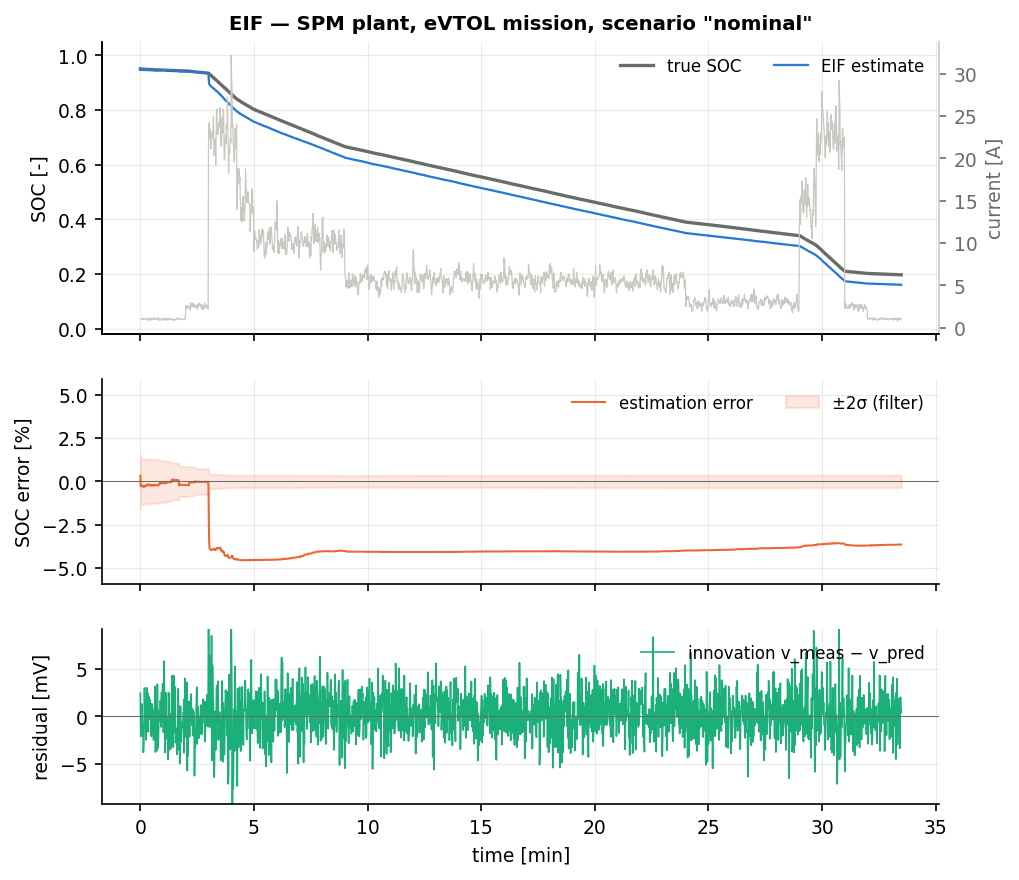
\includegraphics[width=\textwidth]{figures/cellspm_EIF_nominal.png}
\caption{EIF on the nominal mission with the electrochemical (SPM) plant; identical to the conventional EKF.}
\end{figure}
The SPM block of the table is a different kind of test. The plant is the electrochemical
single-particle model; the estimator still runs a 2-RC equivalent circuit, fitted to that plant,
which leaves a \emph{structured} residual of about $4$\,mV (Butler--Volmer kinetics and
solid-phase diffusion that no 2-RC circuit can reproduce) and a slow second branch,
$\tau_2 = 556$\,s. Over a $33$-minute mission a $556$\,s pole barely relaxes, so $v_2(t)$ is
close to an affine ramp --- and so is $\ocv(\soc(t))$ while the cell discharges at a roughly
constant rate. The two channels through which the measurement sees the state,
$(\partial\ocv/\partial\soc)\,\delta\soc$ and $-\delta v_2$, are therefore nearly collinear in
the information accumulated over the flight: the pair $(\soc, v_2)$ is close to unobservable,
and no filter can decide whether a persistent few-millivolt residual belongs to the slow RC
branch or to the state of charge. Because that direction is weakly observable, a $4$\,mV
structured error maps onto \emph{several per cent} of SOC instead of the
$4\,\text{mV}/0.8\,\text{V}\approx0.5\,\%$ a well-conditioned channel would give. This
$(\soc,v_2)$ ambiguity, not the size of the residual, is the mechanism behind the
$3.7$--$4.6\,\%$ band in which the whole classical family sits.

Being algebraically the EKF, the EIF inherits the EKF's SPM rows exactly: $3.65/3.73\,\%$ on
\texttt{nominal} with a voltage residual of only $1.02$\,mV, $7.35\,\%$ on \texttt{cold},
$5.69\,\%$ on \texttt{current\_bias}, $5.31\,\%$ on \texttt{sensor\_dropout}, $3.13\,\%$ on
\texttt{param\_mismatch}, $1.99\,\%$ on \texttt{outliers}. Nothing diverges;
$t_{\text{conv}} = 0$ on every SPM row, because the error is a bias rather than a drift.

The SPM rows are, however, the place where the information form's \emph{structural} argument
becomes concrete. The $(\soc,v_2)$ ambiguity is exactly a near-singular direction of
$\bm{Y}$: the information matrix accumulates almost nothing along it, and the filter's inability
to apportion the residual is visible as a small eigenvalue rather than as a large one in $\mP$.
An information filter makes that diagnosis directly --- monitor $\lambda_{\min}(\bm{Y})$ and
its eigenvector --- and it is also the natural place to fix it, since a second, independent
measurement (a rest-period OCV reading, a neighbouring cell, a temperature-corrected
impedance estimate) enters as an additive term $\mH_i^\T\mR_i\inv\mH_i$ that fills in precisely
the missing direction. That is the argument for the information form on this problem, and it is
an architectural one, not a numerical one.

\section{Summary}
The extended information filter is the EKF in inverse-covariance coordinates: the same estimates
to $10^{-11}$, a measurement update that is a plain sum of per-sensor terms, and a time update
that costs three matrix inversions. Use it when measurements arrive from many independent
sources that must be fused without a central sequencing order (pack-level fusion, federated
architectures), when the initial state is genuinely unknown and $\bm{Y}_0 = \bm0$ is the honest
prior, or when you want to reason directly about which directions of the state space the
measurements actually inform --- as the SPM rows show, that is sometimes the real question. Do
not use it for a single-sensor, low-dimensional problem with a dense $\mQ$: on this benchmark it
is $2.6\times$ the cost of the EKF for identical results, and slightly worse conditioned.

